% ============================================================
% Author: Yuri van der Burg
% Description: Main LaTeX file for my master thesis
% ============================================================

\documentclass[11pt]{article}
\usepackage[utf8]{inputenc}
\usepackage[english]{babel}
\usepackage[backend=biber, style=phys, citestyle=phys, biblabel=brackets, maxbibnames=5, minbibnames=2]{biblatex}
\addbibresource{references.bib}
\usepackage{graphicx}
\usepackage{comment}
\usepackage{amsfonts}
\usepackage{amssymb}
\usepackage{bbold}
\usepackage{physics}
\usepackage{hyperref}
\usepackage{subcaption}
\usepackage{csquotes} % Recommended by the Log (?)
\usepackage{amsmath}
% Hypersetup - Add hyperlinks, but remove ugly red boxes
\hypersetup{
    colorlinks=true,
    linkcolor=black,
    filecolor=black,      
    urlcolor=black,
    citecolor=black,
    pdftitle={Master Thesis - Yuri van der Burg}
    }
\AtEveryBibitem{\clearfield{note}}


%--------------------- New commands ---------------------
\newcommand{\Lagr}{\mathcal{L}}
\newcommand{\fsl}[1]{{\ooalign{\(#1\)\cr\hidewidth\(/\)\hidewidth\cr}}}
\newcommand{\refeq}[1]{(\ref{#1})}

\numberwithin{equation}{section} % Makes equations numbered as <chapter>.<equation>


%--------------------- Header & Footer ---------------------
\usepackage{fancyhdr}
\setlength{\headheight}{13.6pt}
\renewcommand{\sectionmark}[1]{\markboth{#1}{}} % set the \leftmark
\fancyhf{}
\fancyhead[R]{\textit{Yuri van der Burg}} 
\fancyhead[L]{\leftmark}
\fancyfoot[C]{\thepage}
\renewcommand{\headrulewidth}{0.4pt}


%--------------------- Recommended by Log ---------------------
\DeclareUnicodeCharacter{03B2}{$\beta$}
\DeclareUnicodeCharacter{02B9}{'}
\begin{document}


% ============================================================
%                     Import chapters
% ============================================================

%--------------------- Title page ---------------------
\pagestyle{plain} 
\clearpage
\thispagestyle{empty}
\begin{center}
    
\includegraphics[width=8cm,height=8cm,keepaspectratio]{figures/UZH.png}
    \label{fig:uzh}

	\vspace{2cm}
    \Huge
      Data-Driven Analysis for Improved Signal Detection in LEGEND-200
	\vspace{1.5cm}

    \huge
    Master Thesis in Physics
	\vspace{2cm}

    \Large
      Yuri van der Burg
	  \vspace{2cm}


    \normalsize
    Supervised by \\
    \Large
    Prof. Dr. Laura Baudis \\
    Dr. Marta Babicz \\
	\vspace{2cm}

    \large
    \today
\end{center}
\vspace{\stretch{3}}



%--------------------- Abstract ---------------------
\clearpage
\begin{center}
\section*{Abstract}
\end{center}
Neutrinoless double beta decay is a hypothesized nuclear process whose observation would have far-reaching implications for particle physics, providing insight into the fundamental nature of neutrinos and the possible violation of lepton number conservation. 
The Large Enriched Germanium Experiment for Neutrinoless double beta Decay (LEGEND) experiment aims to detect this rare decay using high-purity germanium detectors enriched in $^{76}$Ge, where pulse shape discrimination plays a critical role in suppressing background events. 

This thesis presents the development and application of a novel pulse shape discrimination algorithm using a Transformer-based neural network trained on time-series charge waveforms. 
The pulse shape discrimination efficiency at the energy corresponding to the neutrinoless double beta decay signal was evaluated using data from Inverted Coaxial Point Contact detectors produced by Mirion Technologies. The Transformer-based classifier achieved an efficiency of $(86.7 \pm 1.3)$\%, which is consistent with the $(84.3 \pm 0.5)$\% obtained using the conventional A/E method, where A/E is the ratio of the maximum current amplitude to the reconstructed energy. A two-sided $p$-value of $p \approx 0.08$ indicates no significant difference between the two approaches at the 5\% level. The total detection efficiency achieved with the Transformer-based approach is $(66.8 \pm 2.1)$\%, compared to $(65.0 \pm 2.0)$\% for the A/E method. 
A Bayesian statistical framework is employed to propagate uncertainties in the efficiency and evaluate the resulting impact on LEGEND's neutrinoless double beta decay discovery sensitivity. 

If LEGEND-200 -- the first of two stages of the LEGEND experiment, with a total target mass of 200~kg -- reaches its design goals of a background index of $2 \times 10^{-4}$~counts/(keV$\cdot$kg$\cdot$yr) and a total exposure of $1000 \; \mathrm{kg} \cdot \mathrm{yr}$, the projected sensitivity to the neutrinoless double beta decay half-life is $T^{0 \nu}_{1/2} = 1.22^{+0.33}_{-0.37} \times 10^{27}$~yr for A/E and $T^{0 \nu}_{1/2} = 1.25^{+0.34}_{-0.37} \times 10^{27}$~yr for the Transformer-based method. 

While the Transformer-based classification does not yet significantly enhance the experimental sensitivity, it demonstrates the potential of advanced machine learning techniques in improving background rejection and sensitivity. Further development and validation, such as through refined data cleaning procedures, better balanced training sets, and enhanced detector-specific modeling, are required to consistently outperform conventional methods. 
Continued progress along these lines could pave the way for the robust integration of machine learning models into the LEGEND analysis workflow, ultimately helping to maximize discovery sensitivity.



%--------------------- Contents ---------------------
\clearpage
\tableofcontents 


%--------------------- Introduction ---------------------
\clearpage
\pagestyle{fancy} 
\section{Introduction}
\label{sec:01_introduction}

Neutrino physics lies at the forefront of modern particle physics, addressing some of the most fundamental questions about the nature of matter and the evolution of the universe. One of the most compelling processes in this context is neutrinoless double beta ($0 \nu \beta \beta$) decay. 
Its observation would confirm that neutrinos are Majorana particles, with profound implications for our understanding of fermion mass generation. As a direct consequence, it would imply the violation of lepton number -- a necessary condition for baryogenesis via leptogenesis, which may explain the observed matter-antimatter asymmetry in the universe. 
While the sensitivity of $0 \nu \beta \beta$ decay to the absolute neutrino mass scale is model-dependent, a null result at high exposure would still provide strong and complementary constraints, especially when combined with limits from cosmology and beta-decay experiments. The process would appear as a monoenergetic peak at $Q_{\beta \beta}$. To search for this rare process with the required sensitivity, the LEGEND experiment was conceived as a phased program, with LEGEND-200 now operational and using modular arrays of high-purity germanium (HPGe) detectors enriched in $^{76}$Ge. 
To reach its background goal of $10^{-5}$~counts/(keV$\cdot$kg$\cdot$yr), LEGEND combines ultra-clean detector materials with powerful analysis techniques. A crucial element in this effort is pulse shape discrimination (PSD), which enables the rejection of multi-site and surface background events by analyzing the shape of recorded waveforms. 
Traditionally, PSD relies on hand-engineered features such as the ratio between area and energy (A/E). However, such approaches can be sensitive to electronic noise and calibration drifts, and may not fully exploit all the discriminative information in the waveform. 
This motivates the use of machine learning techniques -- particularly Transformer architectures -- which employ self-attention mechanisms to model long-range dependencies in sequential data, enabling the automatic extraction of rich, high-dimensional correlations from raw waveform data. Such models may improve discrimination performance beyond conventional methods.

\noindent The structure of this thesis is as follows: 

Chapter~\ref{sec:02_neutrino} establishes the theoretical motivation for this work. It introduces neutrinos within and beyond the Standard Model, motivating the search for neutrinoless double beta decay as a probe of the Majorana nature of neutrinos. The chapter concludes by summarizing the landscape of current and future neutrino experiments. 

Chapter~\ref{sec:03_legend} addresses the experimental realization of such searches in the LEGEND experiment. It explains how HPGe detectors are used to achieve the required sensitivity, focusing on signal formation and the challenge of background suppression. Pulse shape discrimination is introduced as a key strategy, and the chapter concludes with an overview of the experiment's calibration procedures. 

Chapter~\ref{sec:04_transformer} covers the machine learning concepts relevant to this work, focusing on deep learning. It justifies applying deep learning to PSD and motivates the use of Transformers as particularly well-suited for waveform data. The chapter concludes with a discussion of the Transformer architecture and the specific model used in this thesis. 

Chapter~\ref{sec:05_PSD_efficiency} describes the practical implementation of a Transformer-based PSD method. It details the LEGEND-200 data processing, the preparation of training data for the Transformer models, their configurations, and their performance. The extraction of PSD efficiencies at $Q_{\beta \beta}$ is also described, and an overview of the current status of pulse shape simulation in LEGEND-200 is presented. The chapter concludes with a brief summary of the key results. 

Chapter~\ref{sec:06_Sensitivity} presents the Bayesian sensitivity study used to quantify the impact of the PSD methods on the attainable $0 \nu \beta \beta$ half-life. It introduces the statistical framework and outlines the procedure used in this work to translate detector performance into projected half-life sensitivities. It concludes with a concise summary of the results. 


The thesis concludes with a discussion of the results, including limitations and possible directions for further improving PSD methods. 


%--------------------- Neutrino physics ---------------------
\clearpage
\section{Neutrino physics} 
\label{sec:02_neutrino}
This chapter covers relevant concepts for $0 \nu \beta \beta$ decay searches. It begins with an introduction to the Standard Model, explaining why its minimal formulation cannot account for neutrino masses. It then presents evidence that neutrinos can change flavor during propagation, implying that neutrinos can not be massless. 
Next, it discusses two different mechanisms for generating neutrino masses, considering neutrinos as Dirac or Majorana particles. After a brief theoretical introduction to $0 \nu \beta \beta$ decay, several experimental results are discussed. 
The chapter concludes with the introduction of the next-generation $0 \nu \beta \beta$ decay experiments.

\subsection{Neutrinos in the Standard Model of particle physics}
The last few centuries of physics research have concluded that there are four fundamental interactions in nature: gravity, described by the theory of general relativity, and the electromagnetic, weak, and strong interactions. The latter three are unified in the framework of the Standard Model of particle physics (SM), a gauge quantum field theory in which particles arise as quantized excitations of the underlying fields~\cite{peskin_introduction_2019}. 

The total gauge symmetry of the SM is $SU(3)_C \times SU(2)_L \times U(1)_Y$. The $SU(3)$ component of the SM is related to quantum chromodynamics, the theory of the strong force. 
It describes how quarks, carrying color charge, are confined to form hadrons. The remaining part of the SM gauge symmetry corresponds to the unification of the electromagnetic and the weak interaction. The $L$ indicates that the weak interaction couples to left-handed particles, as only left-handed fermions (and right-handed anti-fermions) participate in weak-isospin doublets. The group $U(1)_Y$ is associated with the weak hypercharge $Y$. 

In the SM, there are three generations of leptons: The three charged leptons $e$, $\mu$, and $\tau$ and their corresponding neutrinos ($\nu_e, \nu_\mu, \nu_\tau$). These leptons are grouped into $SU(2)_L$ doublets for the left-handed components. Usually, $l_L$ denotes an unspecified $SU(2)_L$ doublet while $l_R$ refers to the corresponding right-handed singlet, which does not participate in weak-isospin interactions:

\begin{equation} 
\label{eq:su2_leptonic_doublets}
l_L = 
	\begin{pmatrix} \nu_{\text{l}} \\ \text{l} \end{pmatrix}, \; 
    l_R = \text{l}_R \,.
\end{equation}

\noindent Here, $\text{l}$ represents one of the charged leptons and $\nu_l$ its corresponding neutrino.
The four generators of the electroweak gauge symmetry, corresponding to $SU(2)_L$ and $U(1)_Y$, do not directly correspond to physical particles. Instead, specific linear combinations of these generators give rise to the physical gauge bosons of the weak and electromagnetic interactions. 
Two $SU(2)_L$ gauge bosons form the charged weak gauge bosons $W_{\mu}^{\pm}$, which mediate charged current (CC) interactions such as $\beta$-decays. The Lagrangian is given in~\refeq{eq:Lagr_weak_CC}, where $\gamma^{\mu}$ represents the Dirac matrices and $g$ denotes the weak coupling constant. The notation $\overline{\nu_{l, L}} = (\nu_{l, L})^\dagger \gamma^0$ and $\overline{l^{-}_{L}} = (l_L)^\dagger \gamma^0$ denotes the Dirac adjoint of the left-handed neutrino and lepton fields, respectively.

\begin{equation}
\label{eq:Lagr_weak_CC}
    \Lagr_{CC} = - \frac{g}{\sqrt{2}} \sum_l \left( \overline{\nu_{l, L}} \gamma^{\mu} l^{-}_{L} W^{+}_{\mu} + \overline{l^{-}_{L}} \gamma^{\mu} \nu_{l, L} W^{-}_{\mu} \right) \,.
\end{equation}

The remaining $SU(2)_L$ gauge boson, $W^3_{\mu}$ mixes with the $U(1)_Y$ gauge boson to form the electrically neutral $Z_{\mu}$ boson and the photon, $A_{\mu}$, according to the following relation

\begin{equation}
\label{eq:weak_mixing}
\begin{pmatrix}
    Z^0_{\mu} \\ A_{\mu}
\end{pmatrix}
= \begin{pmatrix}
    \cos \theta_W \; - \sin \theta_W \\
    \sin \theta_W \; + \cos \theta_W 
\end{pmatrix}
\begin{pmatrix}
    W^3_{\mu} \\ B_{\mu}
\end{pmatrix} \,,
\end{equation}

\noindent where $W^3_{\mu}$ is the third gauge boson of the $SU(2)_L$ group, $B_{\mu}$ is the gauge boson of the $U(1)_Y$ group, and $\theta_W$ is the weak mixing angle~\cite{weinberg_quantum_1995, navas_review_2024}. 
The $Z^0_{\mu}$ boson mediates weak neutral current (NC) interactions, with the corresponding Lagrangian given in equation~\refeq{eq:Lagr_weak_NC}. Weak NC interactions depend on the weak hypercharge and therefore couple also to right-handed fermions (and left-handed anti-fermions). 
However, in the minimal Standard Model, right-handed neutrinos do not exist, as they are completely uncharged under the gauge interactions.

\begin{equation}
\label{eq:Lagr_weak_NC}
    \Lagr_{NC} = - \frac{g}{2 \cos \theta_W} \sum_l \overline{\nu_{l, L}} \gamma^{\mu} \nu_{l, L} Z^0_{\mu} \,.
\end{equation}


In the unbroken electroweak theory, all gauge bosons and fermions are massless. However, the introduction of the Higgs field $\phi$, a complex scalar doublet, leads to spontaneous symmetry breaking of the $SU(2)_L \times U(1)_Y$ gauge symmetry. This mechanism generates masses for $W^{\pm}$ and $Z^{0}$ bosons, while leaving the photon massless. 
When the Higgs field acquires a non-zero vacuum expectation value $\langle\phi \rangle  = \frac{1}{\sqrt{2}} \begin{pmatrix} 0 \\ v \end{pmatrix}$, the symmetry is spontaneously broken and the weak gauge bosons acquire mass. The mass of the charged weak bosons is given by

\begin{equation}
\label{eq:W_boson_mass}
    m_W = \frac{1}{2} g v \,,
\end{equation}

\noindent where $g$ is weak coupling constant and $v \approx 246$~GeV is the Higgs vacuum expectation value~\cite{navas_review_2024}. 
At energies much lower than $m_W$, the exchange of a virtual $W$ boson can be approximated by a point-like interaction. The corresponding coupling strength is the Fermi constant $G_F$, defined as

\begin{equation}
\label{eq:Fermi_constant}
    G_F = \frac{\sqrt{2}}{8} \frac{g^2}{m_W^2} \approx 10^{-5} \mathrm{GeV}^{-2} \,.
\end{equation}

This low-energy limit reproduces the structure of Fermi's original theory of beta decay, in which weak interactions are modeled as point-like four-fermion interactions with a universal coupling constant~\cite{peskin_introduction_2019}.

Fermion masses are generated through interactions with the Higgs field via the Yukawa coupling. The Yukawa coupling for the electron is described by equation~\refeq{eq:Lagr_Yukawa_e}, where the Hermitian conjugate of the Higgs field is indicated by $\phi^\dagger$ and the Yukawa coupling constant for the electron by $Y_e$~\cite{peskin_introduction_2019}:

\begin{equation} 
\label{eq:Lagr_Yukawa_e}
		\Lagr_Y^e = -Y_e \left( \overline{l_L} \phi l_R + \overline{l_R} \phi^{\dagger} l_L \right) \,.
\end{equation}

When the Higgs field acquires a non-zero vacuum expectation value, the symmetry is spontaneously broken and the electron acquires a mass term proportional to both the Yukawa coupling constant and the vacuum expectation value of the Higgs field~\cite{bilenkij_introduction_2018, navas_review_2024}:

\begin{equation} 
\label{eq:electron_mass}
		m_e = Y_e \cdot \frac{v}{\sqrt{2}} \,.
\end{equation}


This mechanism applies analogously to other fermions, with each particle's mass depending on its specific Yukawa coupling constant. However, since right-handed neutrinos are completely uncharged in the electroweak theory, it is not possible to construct a Yukawa term analogous to~\refeq{eq:Lagr_Yukawa_e}. As a result, the Standard Model predicts that neutrinos are massless~\cite{navas_review_2024}. 

\subsection{Neutrino oscillation}

Already in 1967, Pontecorvo proposed a mechanism where lepton flavor is not conserved during neutrino propagation, leading to the phenomenon known as neutrino oscillation~\cite{pontecorvo_neutrino_1968}. Since then, several experiments have observed deficits in neutrino fluxes from the sun (solar neutrinos), the atmosphere (atmospheric neutrinos), nuclear reactors and particle accelerators, providing strong evidence for neutrino oscillation. In addition to these disappearance signals, later experiments such as OPERA and NOvA have directly observed the appearance of different neutrino flavors, confirming the oscillation mechanism through both disappearance and appearance channels~\cite{opera_neutrino_2019, Acero_nova_2022}.

Atmospheric neutrinos are produced in collisions of cosmic rays with nuclei from the upper atmosphere. The flux is dominated by leptonic pion decays, yielding an expected ratio of:

\begin{equation}
\label{eq:Neurino_flux_ratio}
    \frac{\Phi_{\nu_\mu} + \Phi_{\overline{\nu}_{\mu}}}{\Phi_{\nu_e} + \Phi_{\overline{\nu}_e}} \approx 2 \,.
\end{equation}

The first precise measurement for neutrino oscillation was presented in 1998 by the Super-Kamiokande experiment, a 50 kiloton water Cherenkov detector equipped with over 11'000 photomultiplier tubes (PMTs), located 1000 meters below ground in Japan. Neutrinos are detected via charged current neutrino scattering and subsequent Cherenkov radiation of the leptons~\cite{super-kamiokande_collaboration_evidence_1998}. 
Super-Kamiokande also detected a smaller than expected solar $\nu_e$ flux originating from different nuclear fusion processes, indicating neutrino oscillation in solar neutrinos~\cite{super-kamiokande_collaboration_solar_2001}. This discrepancy between theoretically predicted and experimentally observed $\nu_e$ flux is called the solar neutrino problem. It was solved by the Sudbury Neutrino Observatory (SNO), which provided a crucial breakthrough by detecting both charged-current and neutral-current interactions. By comparing these interaction rates, SNO showed that the total flux of solar neutrinos agreed with theoretical predictions from the Standard Solar Model, but a substantial fraction had transformed into $\nu_\mu$ and $\nu_\tau$ flavors~\cite{SNO_solar_neutrino_2022}.

In general, a neutrino $\nu_{\alpha}$ is produced in a definitive flavor eigenstate ($\nu_e$, $\nu_{\mu}$, $\nu_{\tau}$) via the weak interaction. This neutrino then propagates through spacetime as a linear superposition of the three mass eigenstates ($\nu_1$, $\nu_2$, $\nu_3$), which are the actual fundamental particles. When a neutrino is later detected, it is again projected onto a specific flavor eigenstate, which may differ from its original production state, leading to the possibility of flavor transitions~\cite{thomson_modern_2013, zuber_neutrino_2020}. 
The flavor eigenstates $\nu_{\alpha}$ and mass eigenstates $\nu_i$ are connected through the unitary Pontecorvo–Maki–Nakagawa–Sakata (PMNS) matrix $\mathcal{U}$:

\begin{equation}
\label{eq:neutrino_eigenstates}
	\ket{\nu_{\alpha}}= \sum_i^3 \mathcal{U} \ket{\nu_i}\,.
\end{equation}

This mixing leads to the phenomenon of neutrino oscillation, where a neutrino can change its flavor as it propagates through space. 
The PMNS matrix is typically parametrized by three mixing angles ($\theta_{12}$, $\theta_{13}$, $\theta_{23}$) and a complex phase $\delta$, which can lead to charge-parity (CP) violation in the lepton sector. CP violation in neutrino oscillations is a key area of current research, as it could provide insights into the matter-antimatter asymmetry of the universe. The parametrization, shown in~\refeq{eq:PMNS_matrix}, uses the shorthand $s_{ij} = \sin \theta_{ij}$ and $c_{ij} = \cos\theta_{ij}$. Although the full PMNS matrix contains 18 real parameters, only four of them are physically observable in neutrino oscillation experiments~\cite{navas_review_2024, thomson_modern_2013}.


\begin{equation}
\label{eq:PMNS_matrix}
	\mathcal{U} = \begin{pmatrix} 
	c_{12} \, c_{13} & s_{12}\, c_{13} & s_{13} \, e^{-i \delta_{CP}} \\ 
	-s_{12} \, c_{23} - c_{12} \, s_{13} \, s_{23} \, e^{i \delta_{CP}} & c_{12} \, c_{23} - s_{12} \, s_{13} \, s_{23} \, e^{i \delta_{CP}} & c_{13} \, s_{23} \\
	s_{12} \, s_{23} - c_{12} \, s_{13} \, c_{23} \, e^{i \delta_{CP}} & -c_{12} \, s_{23} - s_{12} \, s_{13} \, c_{23} \, e^{i \delta_{CP}} & c_{13} \, c_{23} \\ \end{pmatrix} 
\end{equation}

\noindent For two-flavor mixing, the probability of neutrino oscillation is given by:

\begin{equation} 
\label{eq:neutrino_oscillation_prob}
    P_{\alpha \to \beta}(t) = \abs{\bra{\nu_{\beta}} \ket{\nu_{\alpha}(t)}}^2 = \sin^2 \left( 2 \theta \right) \cdot  \sin^2 \left( \Delta m^2_{ij} \cdot \frac{L}{4E} \right) \,,
\end{equation}

\noindent where, $\Delta m^2_{ij} = m^2_i - m^2_j$ is the squared mass difference between mass eigenstates $i$ and $j$, $L$ the distance between source and detection, and $E$ the neutrino energy~\cite{zuber_neutrino_2020}. 
Equation~\refeq{eq:neutrino_oscillation_prob} illustrates that the oscillation probability depends on the squared mass differences, not the absolute masses. Consequently, neutrino oscillations require $\Delta m^2_{ij} \neq 0$, and oscillation experiments cannot determine the absolute neutrino mass scale. 
The mixing angle $\theta$ in the two-flavor oscillation probability arises from the underlying unitary transformation that relates flavor and mass eigenstates, analogous to equation~\refeq{eq:neutrino_eigenstates}. In the absence of CP violation, this transformation reduces to a real, orthogonal matrix with a single parameter (an element of $SO(2)$). The angle $\theta$ determines the amplitude of the oscillation probability~\cite{zuber_neutrino_2020}. 

While the two-flavor approximation is useful for illustrative purposes, a complete description of neutrino oscillations involves three-flavor mixing, incorporating all three mass eigenstates and the full PMNS matrix. This more general framework leads to a richer phenomenology, including interference effects between multiple oscillation modes and potential CP-violating effects. 


\subsection{Dirac and Majorana neutrinos}

The discovery of neutrino oscillation -- and therefore the existence of non-zero masses for the neutrinos -- raises the fundamental question of how neutrinos acquire mass. Two popular mechanisms exist to generate neutrino mass terms:
If neutrinos are Dirac particles, masses can be generated by introducing right-handed neutrinos, which are often called sterile because they do not participate in SM interactions. This allows the construction of a Yukawa coupling term analogous to that of the electron, as shown in equation~\refeq{eq:Lagr_Yukawa_e}, leading to a mass term:

\begin{equation}
\label{eq:Yukawa_neutrino}
    m_{\nu} = \frac{Y_{\nu} v}{\sqrt{2}} \,.
\end{equation}

However, the SM offers no satisfactory explanation for why the neutrino Yukawa couplings (and therefore the neutrino masses) are many orders of magnitude smaller than those of other fermions~\cite{giunti_fundamentals_2007}. 

The second possibility is that neutrinos are Majorana particles, meaning they are their own antiparticles: $ \nu^C = \nu$. In this case, right-handed neutrinos are not required, since the charge-conjugated left-handed neutrino field $\nu^C_L$ transforms as a right-handed field. 
The Majorana condition for a general field is expressed as

\begin{equation} 
\label{eq:majorana_condition1}
    \psi = C \overline{\psi}^T \,,
\end{equation}

\noindent where $C$ is the charge-conjugation operator and $\overline{\psi}^T = (\psi^\dagger \gamma^0)^T$ is the transposed Dirac adjoint of $\psi$. 
If neutrinos are Majorana particles, the total lepton number $L = L_e + L_{\mu} + L_{\tau}$ is not conserved, violating a fundamental symmetry of the Standard Model. This has profound implications for physics beyond the Standard Model, including potential mechanisms such as leptogenesis, which could potentially explain the matter-antimatter asymmetry of the universe~\cite{giunti_fundamentals_2007}. 
Moreover, Majorana neutrinos introduce two additional CP-violating phases, known as Majorana phases, to the PMNS matrix. The full Majorana mixing matrix can be written as

\begin{equation}
\label{eq:Majorana_PMNS_matrix}
    \mathcal{U}^M = \mathcal{U}^D \cdot \text{diag}(1, e^{i \alpha}, e^{i \beta}) \,, 
\end{equation}

\noindent where $\mathcal{U}^D$ is the standard Dirac neutrino mixing matrix, and $\alpha$, $\beta$ are Majorana phases~\cite{zuber_neutrino_2020}. These phases, however, do not affect neutrino oscillation probabilities since they cancel out in the oscillation formula (equation~\refeq{eq:neutrino_oscillation_prob}).
The Majorana mass term for the neutrino is given by

\begin{equation} 
\label{eq:lagr_neutrino_majorana_mass}
    \Lagr^M_{mass} = - \frac{1}{2} m \left( \overline{\nu^C_L} \nu_L + \overline{\nu_L} \nu^C_L \right) \,,
\end{equation}

\noindent where $m$ is the Majorana mass term. 

While this discussion assumes three active neutrino species, extensions with sterile neutrinos are under investigation but are not addressed here. 
A compelling framework that incorporates both Dirac and Majorana mass terms is the Type-1 see-saw mechanism~\cite{yanagida_seesaw_1980}. In this scenario, heavy right-handed neutrino fields are introduced as Standard Model singlets. These fields allow for both Dirac mass terms $m_D$, arising from the Higgs mechanism as in the Dirac sense, and a large Majorana mass term $M_R$ for the right-handed neutrinos. The resulting mass Lagrangian takes the form:

\begin{equation} 
\label{eq:lagr_seesaw_mass}
    \Lagr_{mass} = - \frac{1}{2} \left( \overline{\nu_L} \; \overline{(\nu_R)^C} \right)  \begin{pmatrix}
        0 & m_D \\ 
        m_D^T & M_R
    \end{pmatrix}
    \begin{pmatrix}
        (\nu_L)^C \\ \nu_R
    \end{pmatrix} + \mathrm{h.c.} \,,
\end{equation}

\noindent where the Hermitian conjugate is not explicitly written. Diagonalizing this mass matrix yields two mass eigenstates: a very light neutrino with mass approximately $m_\nu \approx \frac{m_D^2}{M_R}$ and a heavy neutrino with mass $\sim M_R$. The light state predominately corresponds to the observed active neutrino, while the heavy state is mostly sterile and lies far beyond the electroweak scale. 

The see-saw mechanism not only naturally explains the smallness of neutrino masses but also implies that neutrinos are Majorana particles. 
Neutrino oscillation experiments indicate a mass hierarchy characterized by $\Delta m^2_{21} \ll \abs{\Delta m^2_{31}} \simeq \abs{\Delta m^2_{32}}$, leading to two possible mass orderings~\cite{navas_review_2024, thomson_modern_2013, kamland_collaboration_reactor_2013}, which are illustrated in figure~\ref{fig:Neutrino_mass_hierarchy}:

\begin{figure}[t]
    \centering
    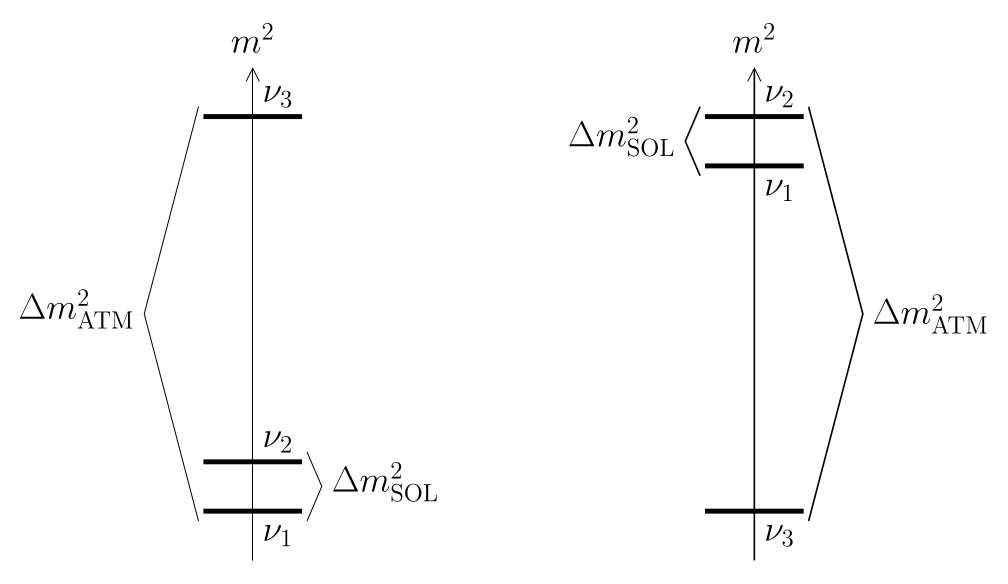
\includegraphics[width=0.85\linewidth]{figures/02_neutrino/Neutrino_mass_hierarchy.png}
    \caption{The two possible neutrino mass hierarchies. Normal ordering is shown on the left and inverted ordering on the right~\cite{giunti_fundamentals_2007}.}
    \label{fig:Neutrino_mass_hierarchy}
\end{figure}

\begin{itemize}
    \item Normal ordering: $m_1 < m_2 \ll m_3$
    \item Inverted ordering: $m_3 \ll m_1 < m_2$
\end{itemize}



\subsection{Neutrinoless double beta decay}
\label{sec:0vbb}

The most promising method to determine whether neutrinos are Dirac or Majorana particles is to search for processes that violate the total lepton number. If such a process is discovered, it would imply that neutrinos are Majorana particles.  
The most sensitive experimental probe for the violation of $L$ is neutrinoless double beta decay, a simultaneous beta decay of two neutrons without emission of neutrinos~\cite{navas_review_2024}. 
Beta decays describe the decay of a neutron into a proton, $(A,Z) \rightarrow (A,Z+1)$ inside a nucleus ($\beta^-$-decay). If $m_{(A, Z+2)} < m_{(A,Z)}$, double beta decay ($2 \nu \beta^- \beta^-$) can occur:

\begin{equation} 
\label{eq:2vbb}
	(A, Z) \rightarrow (A, Z+2) + 2 \, e^- + 2 \, \bar{\nu}_e \,.
\end{equation}

\noindent This is a second-order weak interaction. As such, the decay rate scales as $\Gamma^{2 \nu} \propto G_F^4$, leading to a highly suppressed transition probability. The resulting half-lives are typically of order $T^{2 \nu}_{1/2} \sim 10^{20}$~yr, depending on the nuclear matrix element and available phase space. 
To be experimentally feasible, normal $\beta^{-}$ decay should be energetically forbidden ($m_{(A, Z+1)} > m_{(A, Z)}$)~\cite{zuber_neutrino_2020}. 
Only if neutrinos are Majorana particles, $L$ is not conserved, and neutrinoless double beta decay can occur: 


\begin{equation} 
\label{eq:0vbb}
	(A, Z) \rightarrow (A, Z+2) + 2 \, e^{-} \,.
\end{equation}


\begin{figure}[t]
    \centering
    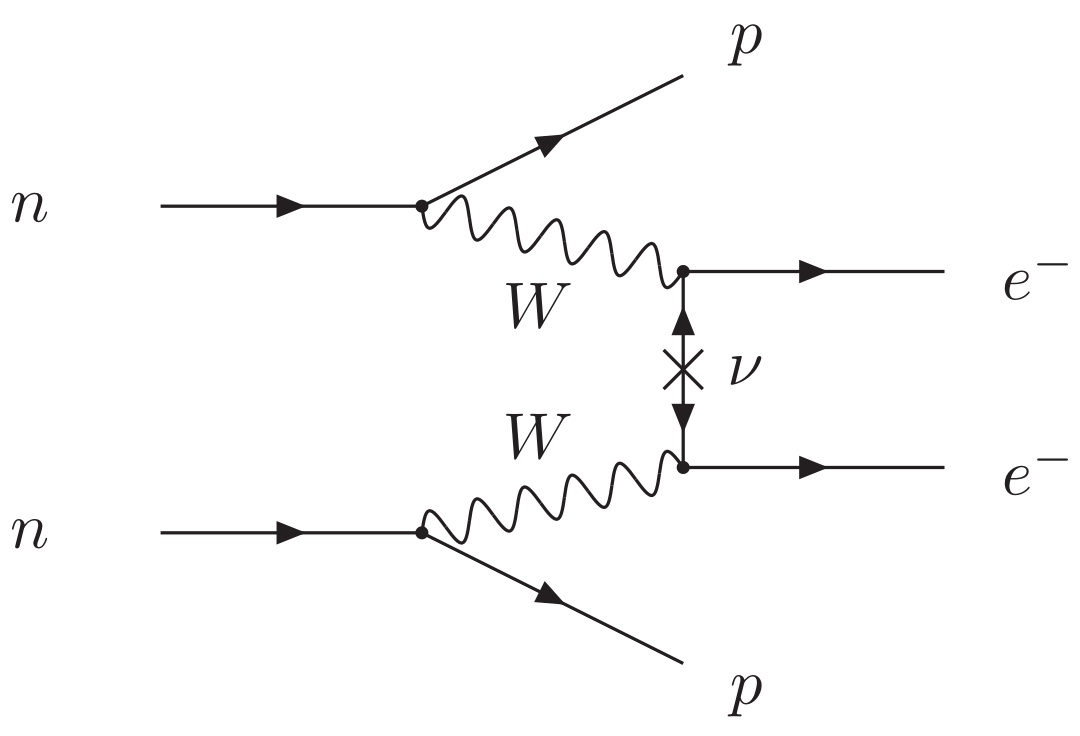
\includegraphics[width=0.75\linewidth]{figures/02_neutrino/feynman_0vbb.png}
    \caption{Feynman diagram of neutrinoless double beta decay: Two neutrons decay into protons and electrons. Only if the neutrino is its own antiparticle, it can be emitted and reabsorbed by a virtual intermediate state, enabling this process~\cite{navas_review_2024}.}
    \label{fig:feynman_0vbb}
\end{figure}


The Feynman diagram for $0 \nu \beta \beta$ decay is shown in figure~\ref{fig:feynman_0vbb} and illustrates why this process is not allowed in the SM: the upper vertex represents $W^{-} \rightarrow e^- + \bar{\nu}_e$ and the lower vertex corresponds to the decay $W^{-} + \nu_e \rightarrow e^-$. Since the exchanged neutrino is emitted as an antineutrino and absorbed as a neutrino, the process is only possible if $\nu_e = \bar{\nu}_e$.

For $0 \nu \beta \beta$ decay, the decay rate $\Gamma^{0 \nu}$ is given by Fermi's golden rule:

\begin{equation} \label{eq:0vbb_halflife}
	\Gamma^{0 \nu} = \frac{\ln 2}{T^{0 \nu}_{1/2}} = \ln 2 \cdot G^{0 \nu}(Q, Z) \cdot \abs{M^{0 \nu}}^2 \cdot \left( \frac{m_{\beta \beta}}{m_e} \right)^2 \,.
\end{equation}

Here, $T^{0 \nu}_{1/2}$ is the half-life, $G^{0 \nu} (Q,Z)$ the phase space factor, and $Q$ the total kinetic energy released. The quantity $M^{0 \nu}$ is the nuclear matrix element, $m_{\beta \beta}$ the effective Majorana mass and $m_e$ the electron mass. The nuclear matrix element $M^{0 \nu}$ carries a model-dependent uncertainty of a factor 2-3~\cite{engel_status_2017}, and the effective Majorana mass is given by:

\begin{equation}
\label{eq:effective_majorana_mass}
    \abs{m_{\beta \beta}} = \abs{\sum_i \mathcal{U}_{ei} ^2m_i} \,
\end{equation}

\noindent where $\mathcal{U}$ is the PMNS matrix and $m_i$ are the mass eigenstates. A full derivation of~\refeq{eq:0vbb_halflife} is presented in~\cite{bilenky_neutrinoless_2015}. 

In this work, we refer to the Q-value of $0 \nu \beta \beta$ decay as $Q_{\beta \beta}$. Furthermore, we define the signal half-rate as

\begin{equation}
\label{eq:signal_half_rate}
    \mathcal{S} = \frac{1}{T^{0 \nu}_{1/2}} \,.
\end{equation}

\noindent This definition of $\mathcal{S}$ corresponds to the half-rate, as it is the inverse of the half-life. This follows the common usage in the field (see~\cite{lnote_25001}, eq.~(8)), where the phase-space factor $G^{0 \nu}$ is defined to include a factor of $1/\ln 2$:

\begin{equation}
\label{eq:0vbb_phase_space}
    G^{0 \nu}(Q,Z) \propto \frac{G_F^4}{\ln 2} \cdot Q_{\beta \beta}^5
\end{equation}


\subsubsection{Experimental searches}

Double beta decay should be observable in 35 isotopes, but due to practical reasons, only 9 are of experimental interest: $^{48}$Ca, $^{76}$Ge, $^{82}$Se, $^{96}$Zr, $^{100}$Mo, $^{116}$Cd, $^{130}$Te, $^{136}$Xe and $^{150}$Nd~\cite{rodejohann_neutrino-less_2011}.
The detection of (neutrinoless) double beta decay is characterized by measuring the kinematic parameters of the emitted electrons~\cite{dolinski_neutrinoless_2019}. 
In the case of $0 \nu \beta \beta$ decay, the total energy carried by the emitted electrons equals the Q-value of the decay (neglecting nuclear recoil), resulting in a monoenergetic peak. 
In practice, this peak is broadened due to the finite energy resolution of the detector. In contrast, $2 \nu \beta \beta$ decay produces a continuous energy spectrum, as the undetected neutrinos carry away varying amounts of energy. 
Figure~\ref{fig:expected_energy_spec} illustrates the expected energy depositions for both decay modes in the transition $^{76} \mathrm{Ge} \rightarrow \, ^{76} \mathrm{Se}$.
The Q-value for this process is $Q_{\beta \beta} = 2039.0612 \pm 0.0075$~keV~\cite{Huang_2021}.

\begin{figure}
    \centering
    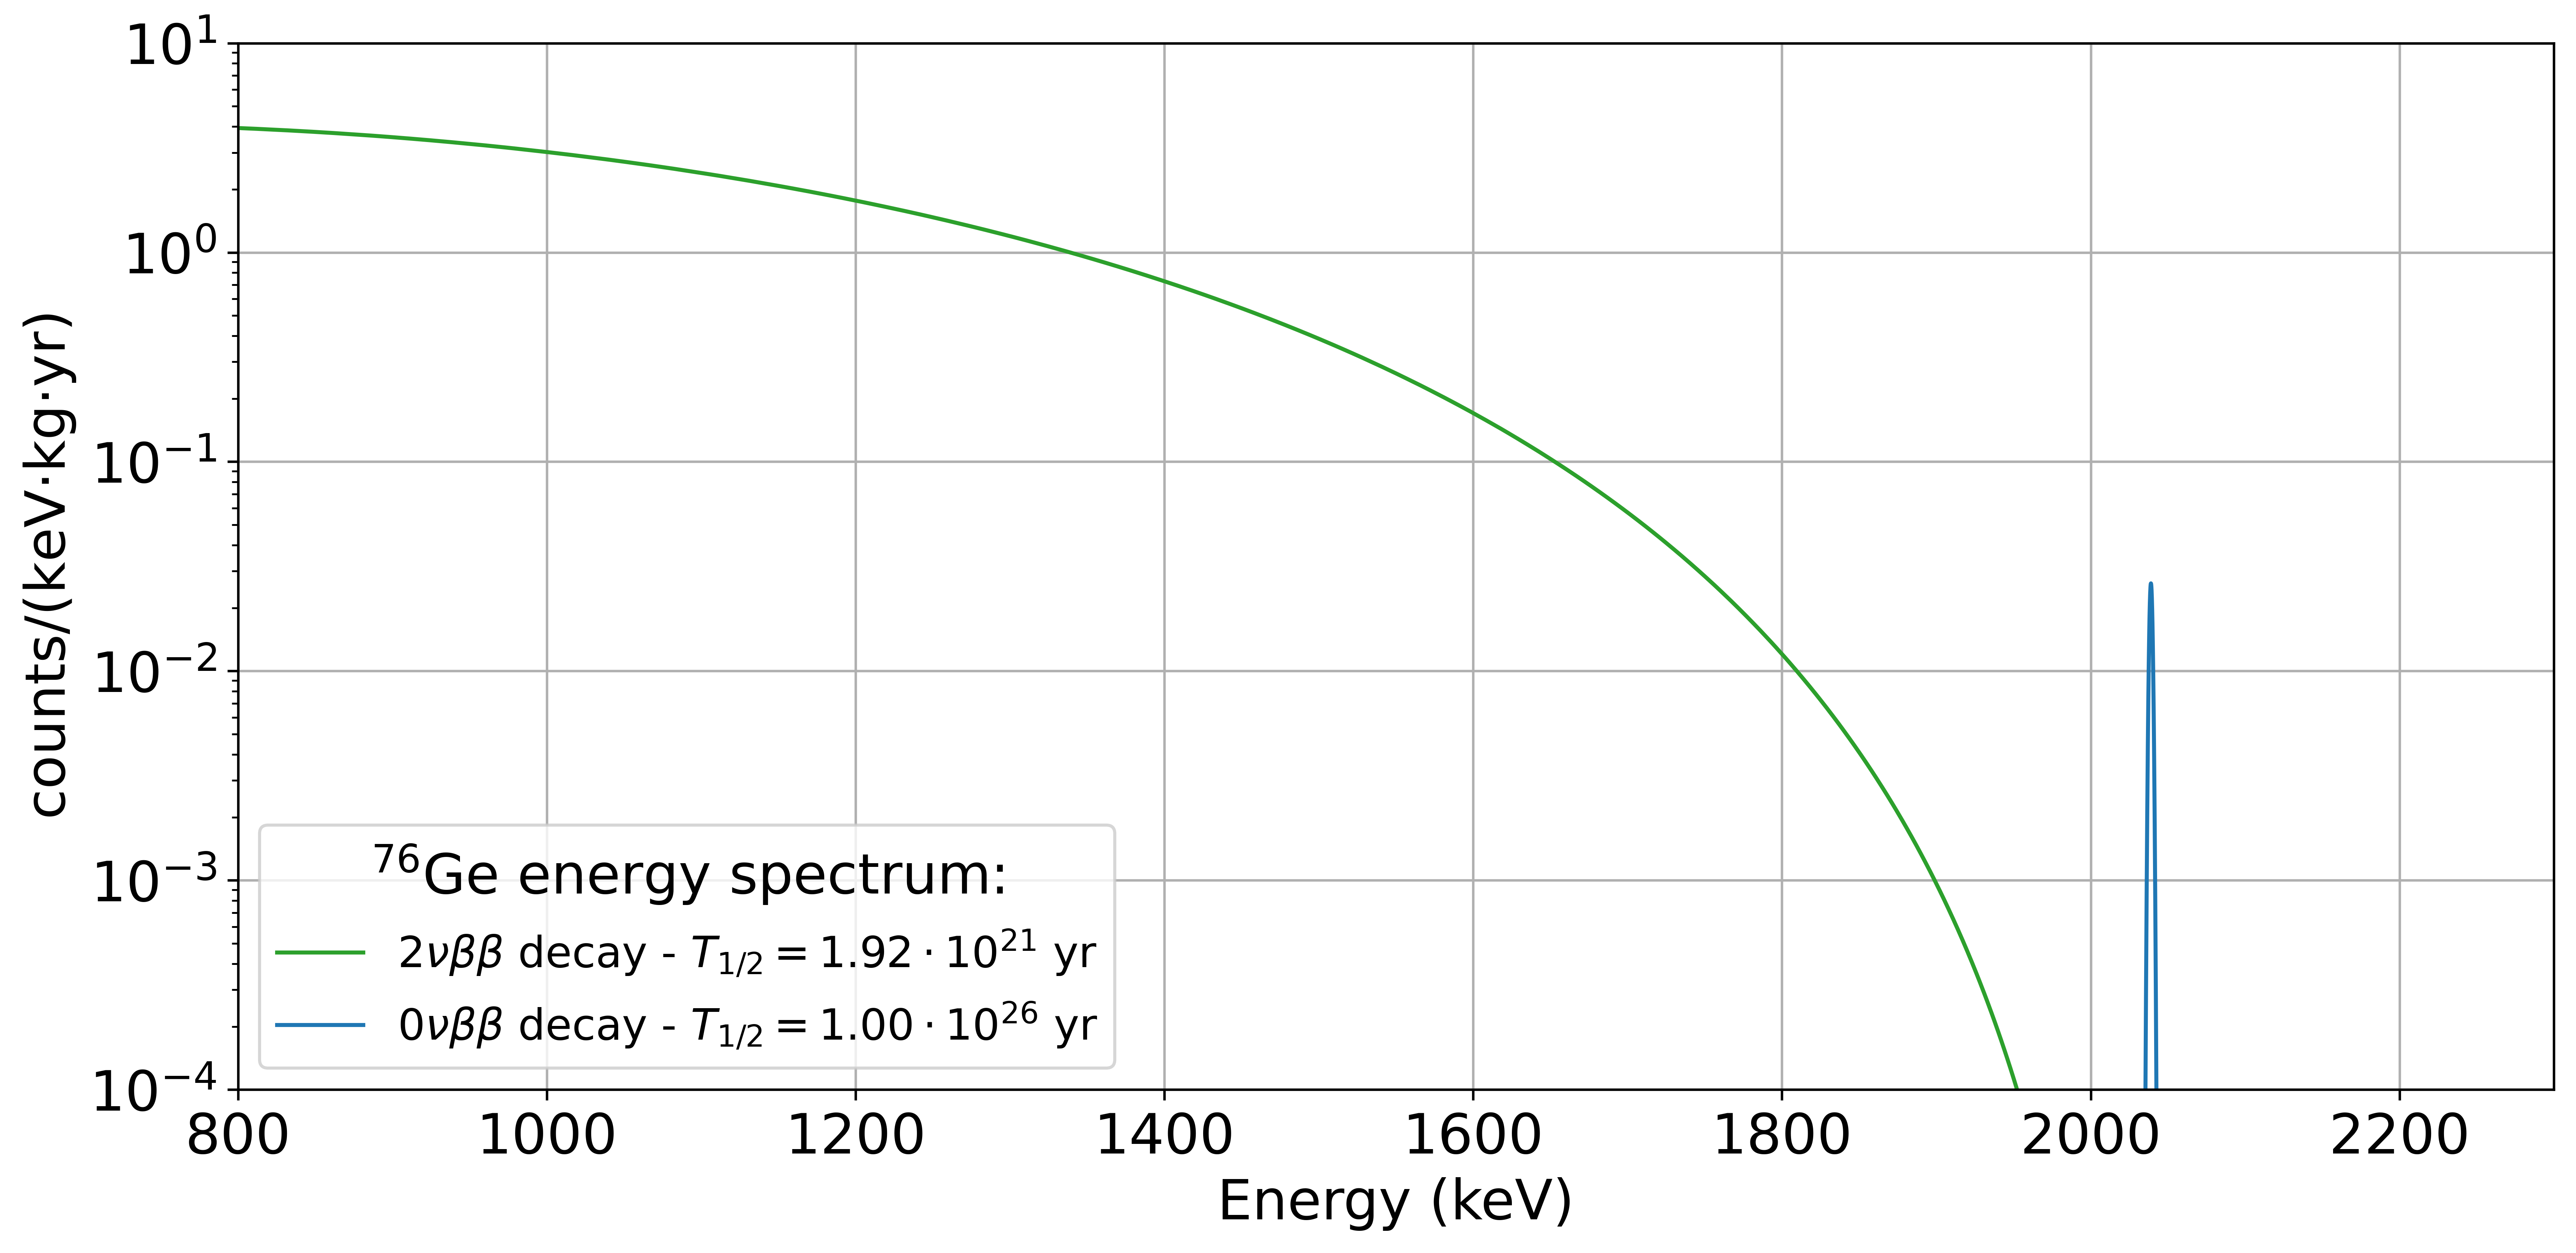
\includegraphics[width=0.95\linewidth]{figures/02_neutrino/Energyspectrum_Ge76.png}
    \caption{Expected energy spectra for $2 \nu \beta \beta$ and $0 \nu \beta \beta$ decay in $^{76}$Ge. The $2 \nu \beta \beta$ decay spectrum is computed using the phase space distribution from \cite{kotila_phasespace_2012}, scaled to a half-life of $1.92 \cdot 10^{21}$~yr. The $0 \nu \beta \beta$ decay signal is modeled as a Gaussian at $Q_{\beta \beta} = 2039$~keV, assuming a detector resolution of FWHM~$= 2.5$~keV and a half-life of $10^{26}$~yr, following the estimates from the GERDA collaboration~\cite{dandrea_neutrinoless_2021}.}
    \label{fig:expected_energy_spec}
\end{figure}


The sensitivity to the half-life depends heavily on the amount of background: 

\begin{equation}
\label{eq:0vbb_hl_sensitivity}
	T^{0 \nu}_{1/2} \propto 
    \begin{cases}
        a \cdot M \cdot \epsilon \cdot t &  \text{background free} \\
        a \cdot \epsilon \cdot \sqrt{\frac{M \cdot t}{B \cdot \Delta E}} &  \text{with background}
    \end{cases}    
\end{equation}

\noindent Here, $a$ is the isotopic abundance, $\epsilon$ the efficiency of the detection, $M$ the total mass used in kg, $t$ the time measured in years, $B$ the background in counts/(keV$\cdot$kg$\cdot$yr), and $\Delta E$ is the energy resolution in keV~\cite{zuber_neutrino_2020, dolinski_neutrinoless_2019}. 
Equation~\refeq{eq:0vbb_hl_sensitivity} shows why it is of utmost importance to achieve a quasi-free background: If there are many background events, the sensitivity scales $(M \cdot t)^{1/2}$ instead of $M \cdot t$. Moreover, the energy resolution must be sufficiently good, otherwise the sharp peak at $Q_{\beta \beta}$ is indistinguishable from the $2 \nu \beta \beta$ decay tail~\cite{delloro_neutrinoless_2016}. 

Neutrinoless double beta decay has not been observed yet. However, several different experiments can constrain the $0 \nu \beta \beta$ decay half-life: 
The KamLAND-Zen consists of a tank filled with a liquid scintillator that contains a balloon of Xenon-loaded liquid scintillator as the $0 \nu \beta \beta$ decay source. Inside the tank are almost 2000 PMTs alongside the walls. KamLAND-Zen achieved $T^{0 \nu}_{1/2} > 2.3 \times 10^{26}$yr with $^{136}$Xe~\cite{kamland-zen_collaboration_search_2023}. 

The CUORE experiment is a cryogenic calorimeter that consists of 988 TeO$_2$ crystals. Energy depositions in the crystals will lead to a temperature rise, which is transformed into an electrical signal. The experiment measured a half-life of $T^{0 \nu}_{1/2} > 2.2 \times 10^{25}$yr using over 200~kg of $^{130}$Te~\cite{adams_search_2022}. Reported values are at $90 \% $ C.L. 

CUPID-Mo, which served as a demonstrator for the upgrade of CUORE, contains enriched Li$_2$MoO$_4$ scintillating calorimeters, obtaining a half-life of $T^{0 \nu}_{1/2} > 1.8 \times 10^{24}$ for $^{100}$Mo~\cite{augier_final_2022}. 


A very promising approach is ionizing radiation detection, as shown by the GERDA and MAJORANA DEMONSTRATOR (MJD) experiments. While not exclusively to these setups, both experiments showed that a HPGe-based approach is highly efficient in terms of energy resolution and intrinsic background suppression due to the detector-source identity~\cite{dandrea_neutrinoless_2021}. 
The GERDA collaboration achieved an unprecedentedly low background of $5.2 \times 10^{-5}$ counts/(keV$\cdot$kg$\cdot$yr) and an exposure-weighted energy resolution of $(2.9 \pm 0.1)$~keV full width half maximum (FWHM) at $Q_{\beta \beta}$ for the detector geometry used in this work
. The final value reported by the GERDA collaboration was $T^{0 \nu}_{1/2} > 1.8 \times 10^{26}$yr at $90\%$ C.L.~\cite{gerda_collaboration_final_2020}.  
MJD reached an impressive energy resolution of $(2.55 \pm 0.09)$~keV FWHM at $Q_{\beta \beta}$, with a final half-life of $T^{0 \nu}_{1/2} > 8.3 \times 10^{25}$ yr at $90 \%$ C.L.~\cite{majorana_collaboration_final_2023}.

In addition to direct searches, complementary constraints on the absolute neutrino mass scale arise from cosmological observations and kinematic measurements. 
The Planck satellite has placed an upper limit on the sum of neutrino masses, currently constrained to $\sum m_\nu < 0.16$~eV at 95\% confidence level under the $\Lambda \mathrm{CDM}$ model~\cite{ivanov_cosmological_2020}. 

On the experimental side, the KATRIN experiment probes the kinematic endpoint of tritium beta decay, directly measuring the effective electron neutrino mass: $m_\nu = \sqrt{\sum \abs{U_{ei}}^2 \, m_i^2}$. Its latest results set an upper limit of $m_{\nu} < 0.8 \,\mathrm{eV} c^{-2}$ at 90\% CL~\cite{aker_direct_2022}.
While not sensitive to the Majorana or Dirac nature, this result further constrains the possible values of $m_{\beta \beta}$, especially in the case of inverted mass ordering. 



\subsection{Current challenges and future prospects}


Assuming three neutrinos, oscillation experiments constrain six parameters: Two mass differences, three mixing angles, and a CP-violating phase. A global analysis of neutrino oscillation data, such as provided by the NuFIT collaboration, yields ever-tighter bounds on these parameters~\cite{esteban_nufit-60_2024}. 

However, oscillation experiments are insensitive to the absolute neutrino mass scale. In this regard, cosmological observation provides a complementary probe: Relic neutrinos affect the large-scale structure of the universe and leave an imprint on the cosmic microwave background through their contribution to the total energy density. 
To determine the neutrino mass hierarchy, neutrinoless double beta decay experiments remain a promising approach, as the measured half-life can be translated into upper limits on the effective Majorana mass -- assuming that the decay is dominated by the exchange of light Majorana neutrinos~\cite{gerda_collaboration_final_2020}.
The sensitivity difference between normal and inverted ordering arises because in the latter case, the two heaviest neutrino mass eigenstates contribute significantly to $m_{\beta \beta}$, leading to a non-zero lower bound. 

For normal ordering, destructive interference between the contributions from the three mass eigenstates can suppress $m_{\beta \beta}$ values close to zero, potentially beyond the reach of upcoming experiments. 
Current limits include $m_{\beta \beta} < 79-180$~meV from GERDA and $m_{\beta \beta} < 36-156$~meV from KamLAND-Zen~\cite{gerda_collaboration_final_2020, abbasi_measurement_2023}. The relatively large range in values reflects uncertainties in the nuclear matrix element involved in the decay process.  

Figure~\ref{fig:Lobster_2024} shows the allowed regions for the effective Majorana masses $m_{\beta \beta}$ as a function of the lightest neutrino mass $m_{\mathrm{min}}$, for both normal and inverted mass ordering. For the inverted hierarchy, next-generation $0 \nu \beta \beta$ decay experiments such as SNO$+$ (using Cherenkov detectors), NEXT (a xenon time projection chamber), or LEGEND (using HPGe detectors) are expected to reach sensitivities that fully probe the relevant parameter space~\cite{agostini_discovery_2017}. \\
Among these, the LEGEND experiment stands out for its combination of excellent energy resolution, ultra-low background techniques and scalability. With its staged approach from LEGEND-200 to LEGEND-1000, the experiment is designed to explore half-lives beyond $10^{28}$ years and approach the full coverage of inverted ordering. 
The next chapter introduces the LEGEND experiment in detail, with an emphasis on the detector technology. 

\begin{figure}
    \centering
    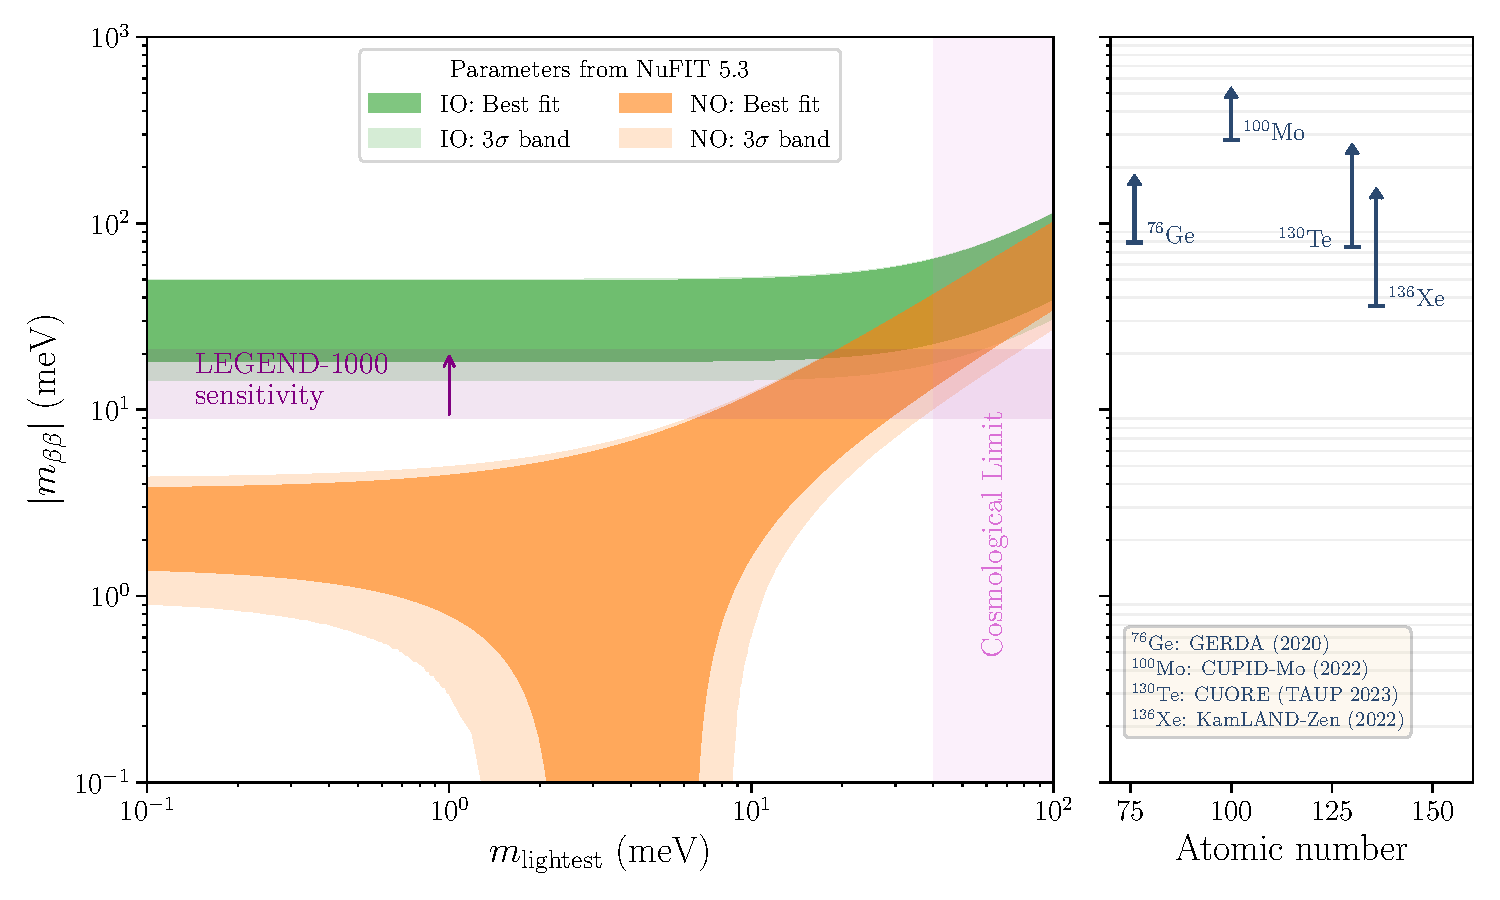
\includegraphics[width=1\linewidth]{figures/02_neutrino/Lobster_plot_NuFIT_5-2.pdf}
    \caption{Left: Effective Majorana mass $m_{\beta \beta}$ for inverted and normal ordering as a function of the lightest neutrino mass $m_\mathrm{min}$, including the projected sensitivity of the LEGEND-1000 experiment. Right: Effective Majorana masses obtained for different isotopes. The figure is created with code from~\cite{torres_toej93lobsterplot_2024}.}
    \label{fig:Lobster_2024}
\end{figure}
 


%--------------------- The LEGEND exp. ---------------------
\clearpage
\section{The LEGEND experiment} 
\label{sec:03_legend}

Following the discussion of neutrino physics and the significance of neutrinoless double beta decay, this chapter introduces the LEGEND experiment, a next-generation effort to search for neutrinoless double beta decay. It builds on the advancements of its predecessors, MJD and GERDA. LEGEND reuses the infrastructure at the Laboratori Nazionali del Gran Sasso (LNGS), previously used by GERDA, and upgrades it to improve both background suppression and detector performance. 
The chapter begins with a short overview of how LEGEND evolved from GERDA and MAJORANA, focusing on key improvements in detector design and instrumentation. It then introduces the high-purity germanium (HPGe) detectors used in the experiment, and the principles of semiconductor physics, including doping and charge collection. Finally, it covers how these detectors are used to identify neutrinoless double beta decay events, how pulse shape discrimination (PSD) helps to reject background, and how the detectors are calibrated in LEGEND-200. 

\subsection{From GERDA to LEGEND}

The GERmanium Detector Array (GERDA) aimed to search for $0 \nu \beta \beta$ decays using high-purity germanium detectors enriched to 87\% in $^{76}$Ge. Located at LNGS, the setup was shielded by 3500 meters of water equivalent of rock, significantly reducing the cosmogenic background.
GERDA operated in two phases. Phase I reached a background index of $10^{-2}$~counts/(keV$\cdot$kg$\cdot$yr) with a total exposure of $21.6 \; \mathrm{kg} \cdot \mathrm{yr}$. The experiment set a new lower limit on the half-life of $T^{0 \nu}_{1/2} > 2.1 \times 10^{25}$yr (90\% CL). 
In phase II, the goal was to improve sensitivity by an order of magnitude. This was addressed by introducing a new detector geometry with better energy resolution and improved pulse shape discrimination (BEGe detectors), as well as a new liquid argon (LAr) veto system and a denser detector array~\cite{agostini_upgrade_2018}. 

In GERDA, the HPGe detectors were attached on strings and submerged in a cryostat filled with 64 m$^3$ LAr, which served both as a coolant and as an active shield against background radiation, including cosmic and environmental radiation. Surrounding the cryostat was a 590 m$^3$ ultra-pure water tank equipped with 66 PMTs providing Cherenkov veto against muons. The clean room was located above the cryostat~\cite{agostini_upgrade_2018}. 
Within the LAr volume, an additional veto system detected energy deposits in both the germanium detectors and the LAr, with scintillation light being measured through wavelength-shifting fibers. These fibers converted the 128 nm scintillation light into green light, directing the photons to silicon photomultipliers for precise detection~\cite{agostini_upgrade_2018}.  

The LEGEND experiment continues from both GERDA and MJD. The idea is to combine GERDA's low background techniques with the high energy resolution of MJD. The final stage, LEGEND-1000, is planned to consist of 1000 kg of germanium and aims for a discovery sensitivity on the order of $10^{28}$ years at $99.7$\% C.L.~\cite{abgrall_large_2017}. 
In a first step, LEGEND-200 aims to employ 200 kg of HPGe detectors inside the existing infrastructure of GERDA, combining it with the low-noise electronics of the MAJORANA experiment, which was achieved by using low-mass front-end electronics close to the detector. The goal is to enter the background-free regime, which is defined as having $< 1$ expected background counts in the region of interest over the experiment's exposure~\cite{collaboration_legend-1000_2021}. For LEGEND-200, this corresponds to a background index of $2 \times 10^{-4} \mathrm{counts / (keV \cdot kg \cdot yr)}$. The design of the LEGEND-200 detector setup is shown in figure~\ref{fig:l200_design}. 

\begin{figure}
    \centering
    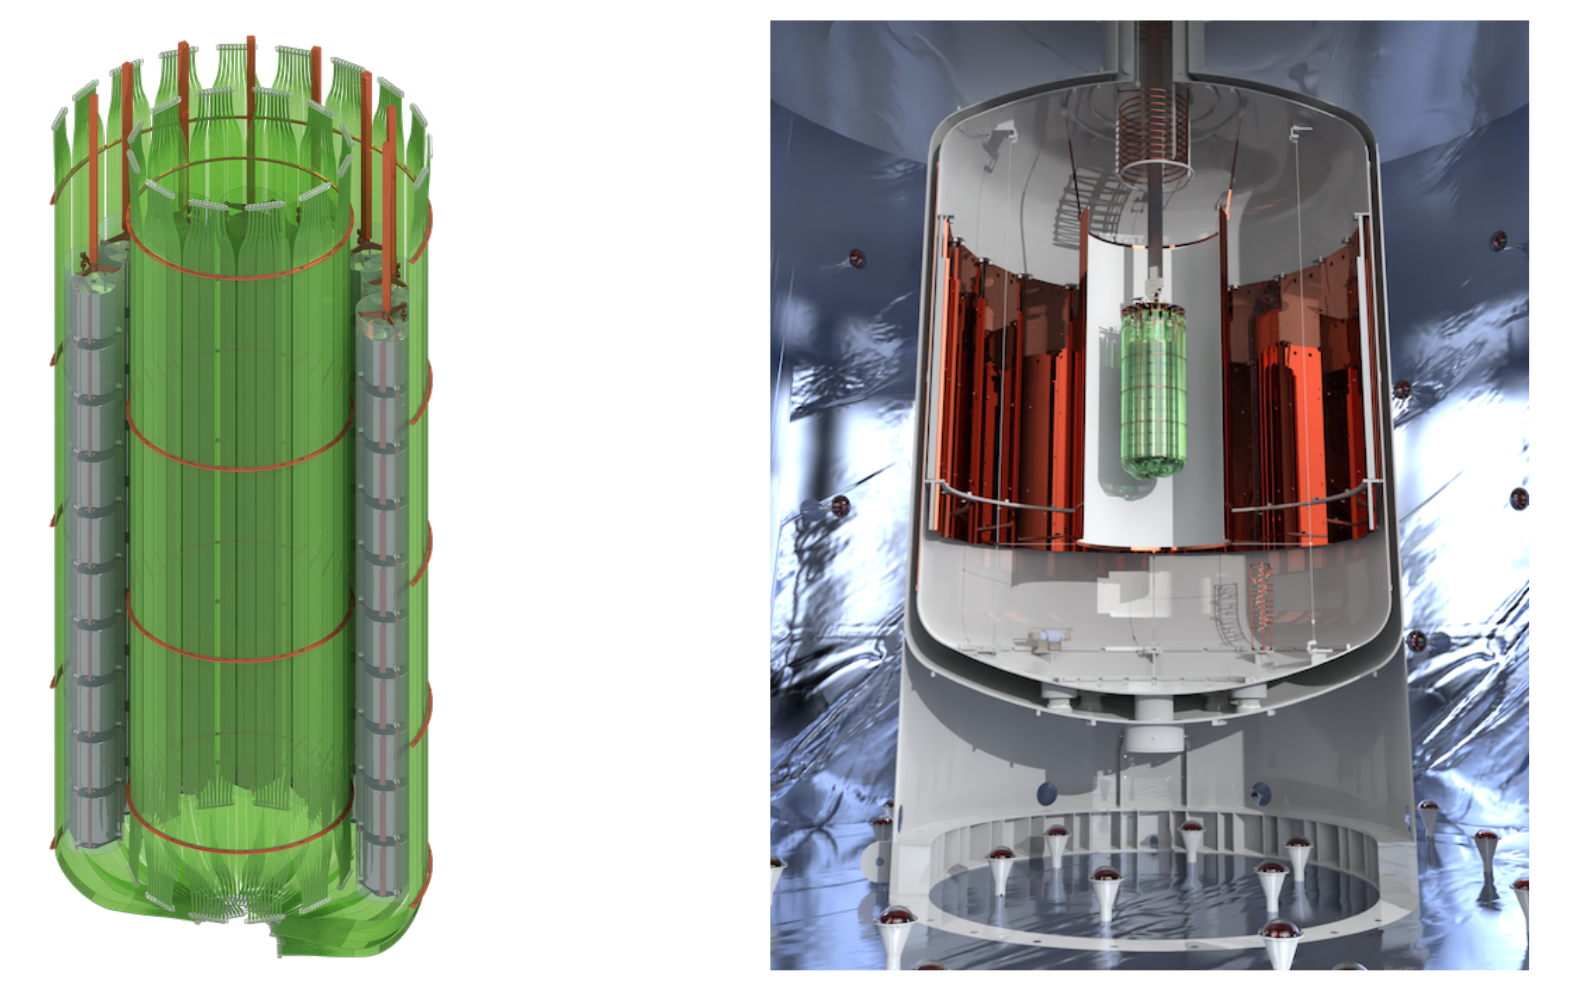
\includegraphics[width=0.8\linewidth]{figures/03_legend/LEGEND_200_design.png}
    \caption{LEGEND-200 design. The left image shows the germanium detectors mounted on the strings, surrounded by optical fibers that guide the LAr scintillation light to silicon photomultipliers. 
	The right image shows the cryostat located in the water Cherenkov tank, which is equipped with PMTs to detect coincident muons~\cite{collaboration_legend-1000_2021}.}
    \label{fig:l200_design}
\end{figure}


\subsection{Germanium detectors}
High-purity germanium detectors are at the core of the LEGEND experiment. Their excellent energy resolution and ability to reconstruct interaction topologies make them particularly well suited for $0 \nu \beta \beta$ decay searches. 

\subsubsection{Germanium semiconductors}
In crystalline solids like germanium, the periodic atomic structure gives rise to a quasi-continuum of energy levels known as energy bands. The valence band is the highest band fully occupied by electrons, while the conduction band is the lowest unoccupied band. The energy difference between these two bands is called the band gap, and its value determines the material's electrical properties. In conductors, the bands overlap; in insulators, the band gap is large. Semiconductors fall in between with band gaps typically below $<3$~eV.  
In the case of germanium, the band gap is $0.67$~eV~\cite{hofmann_solid_2015}. Each atom contributes four electrons that form covalent bonds with neighboring atoms. At zero temperature, the valence band is completely filled and the conduction band is empty, resulting in a very low electrical conductivity. 
However, at non-zero temperatures, thermal excitation can promote electrons into the conduction band, creating electron-hole pairs. Holes represent the absence of electrons in the valence band and act as positively charged carriers. Although the ions themselves are stationary, the movement of holes contributes to electrical conduction~\cite{hofmann_solid_2015, simon_oxford_2017}. 
The law of mass action relates the concentration of electrons $n$ and holes $h$ in a semiconductor at thermal equilibrium: 

\begin{equation}
\label{eq:law_of_mass_action}
	n \cdot p = \text{constant} \,.
\end{equation}

For a perfectly pure semiconductor at room temperature, the charge carrier concentrations are very low, resulting in correspondingly low electrical conductivity. However, in practice, there are always small amounts of impurities present, which increase the number of free charge carriers and thereby the conductivity. 
There are two important types of electronically active impurities: Atoms that act as electron donors are called n-type, while atoms that readily accept electrons (and thus effectively donate holes) are referred to as p-type. 
Semiconductors are typically doped with either type to increase the conductivity to a reasonable value. 
For tetravalent elements like germanium, n-type doping is achieved by introducing pentavalent atoms like phosphorus. The additional outer shell electron cannot participate in a covalent bond and remains only loosely bound to the positively charged nucleus. Its energy level lies just below the conduction band, and only a small amount of thermal energy is required to excite it into the conduction band ~\cite{sze_semiconductor_2012, hofmann_solid_2015, knoll_radiation_2000}. 
P-type doping is achieved by adding trivalent atoms such as boron or aluminium, which act as electron acceptors with energy levels just above the valence band.
At high enough temperatures, where the electrons are no longer bound to the dopant atoms, n-type doping will lead to free electrons and p-type doping leads to free holes, thus increasing the free charge carrier concentration in either case. Regions with very high doping concentrations are particularly well suited for electrical contacts due to their high conductivity. These regions are referred to $n^{+}$ and $p^{+}$, depending on the type of impurity introduced~\cite{simon_oxford_2017, knoll_radiation_2000}. 


\subsubsection{Semiconductors as particle detectors}
If p-type and n-type semiconductors are brought into direct contact, the concentration gradient causes electrons to diffuse into the p-doped region, while holes diffuse towards the n-doped region. In the overlapping region, known as the depletion zone, electrons and holes recombine. For each electron that diffuses away from the n-doped side, a net positive charge remains due to the immobile donor impurity. 
Analogously, for every hole that diffuses out of the p-doped side, an immobile acceptor impurity remains. This charge imbalance creates an electric field across the depletion region, which acts to counter further diffusion until equilibrium is reached~\cite{knoll_radiation_2000, simon_oxford_2017}. 
The depletion region contains almost no free charge carriers and therefore exhibits very high resistivity. 


\begin{figure}[t]
    \centering
    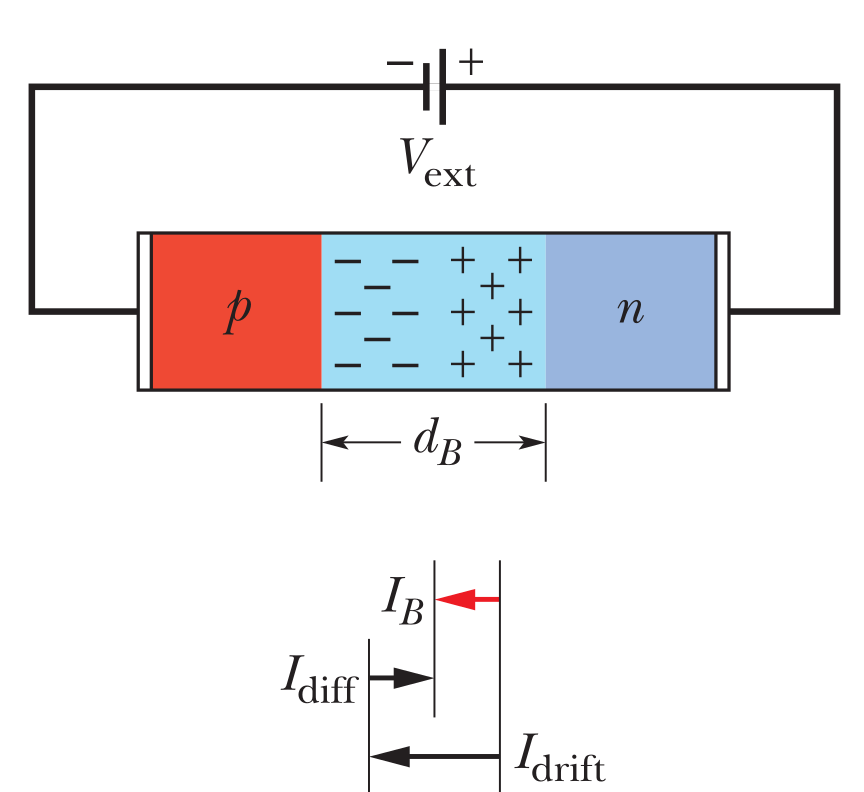
\includegraphics[width=0.5\linewidth]{figures/03_legend/PN_junction.png}
    \caption{Schematic view of a p-n junction in reverse bias. Since the applied voltage opposes the direction of the diffusion $I_{\text{diff}}$, only a small current $I_B$ remains. As a result, the depletion zone $d_B$ widens and the conductivity decreases~\cite{walker_fundamentals_2014}.}
\label{fig:pn_junction}
\end{figure}

 
An external voltage can be applied across the junction in either direction: 
When the voltage is applied in the same direction as the concentration difference (i.e., opposite the existing electric field), the junction is said to be in forward bias. In this case, electrons can move easily from the n-doped to the p-doped region, and the conductivity increases. 

The reverse case is more relevant for particle detection. In reverse bias, which is shown in figure~\ref{fig:pn_junction}, the external voltage is applied in the same direction as the existing electric field, opposing the natural diffusion of charge carriers. This pulls electrons from the p-doped region toward the n-side. Since the carrier concentrations are already low, the current is greatly suppressed, and the depletion region widens ~\cite{hofmann_solid_2015, knoll_radiation_2000, simon_oxford_2017}.

When ionizing radiation interacts in the depletion zone of a reverse-bias semiconductor, it deposits energy and generates a number of electron-hole pairs within a few picoseconds~\cite{agostini_pulse_2022}. 
These charge carriers are separated by the electric field and drift towards their respective electrodes, inducing a measurable signal. Due to the low ionization energy in semiconductors, detectors of this type achieve a high signal-to-noise ratio. 
The probability for such interactions, and its dependence on photon energy in germanium, is illustrated in figure~\ref{fig:Ge_attenuation}, which shows the mass attenuation coefficient for germanium, including prominent K- and L-shell absorption edges. 

\begin{figure}
    \centering
    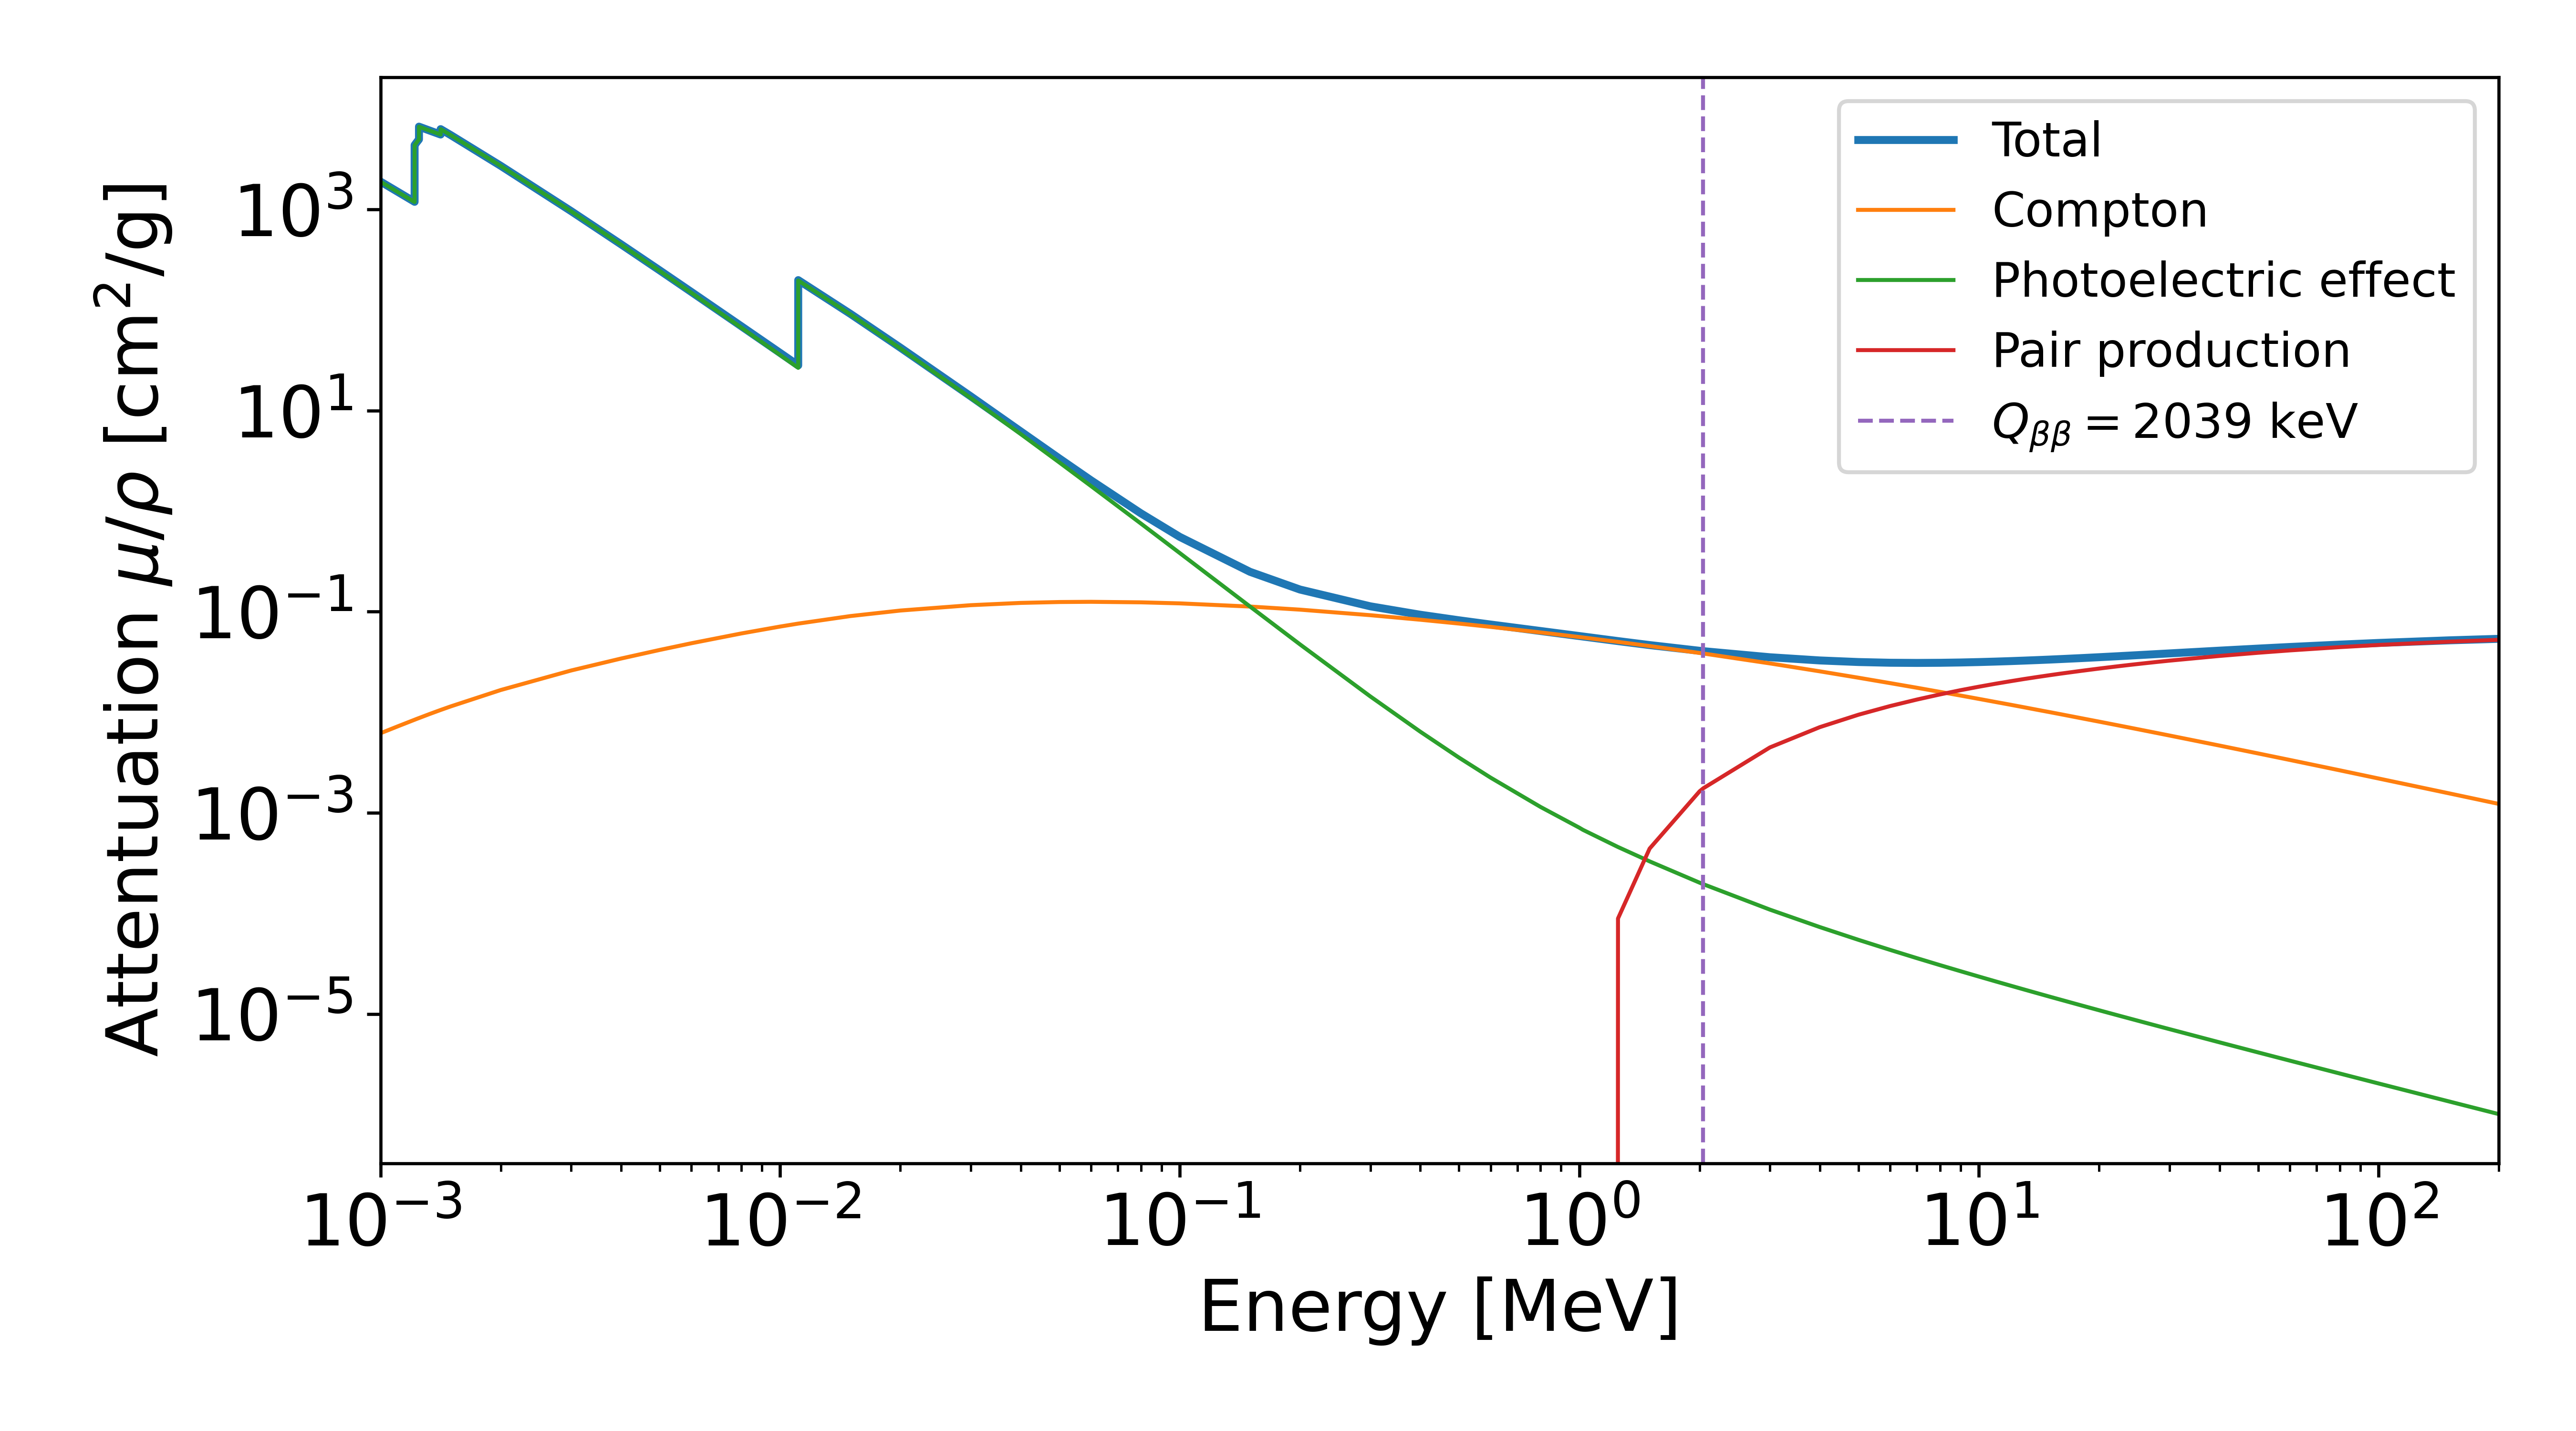
\includegraphics[width=0.75\linewidth]{figures/03_legend/Attentuation_germanium.png}
    \caption{Mass attenuation coefficients for germanium, showing contributions from photoelectric absorption, incoherent (Compton) scattering, and pair production, along with the total attenuation. The region of interest around $Q_{\beta \beta}$ (horizontal line) is dominated by Compton scattering. Data from NIST XCOM~\cite{nist_xcom_1999}.}
\label{fig:Ge_attenuation}
\end{figure}

In HPGe detectors, the applied reverse bias is large enough to deplete almost the entire detector volume, but still below the breakdown voltage. The small region that remains undepleted is referred to as dead layer, where charge collection is incomplete and signals are suppressed~\cite{knoll_radiation_2000}. 

The electron-hole pairs created during an interaction inside the detector drift toward the electrodes in a few microseconds. 
While in principle signals can be read out from either p$^+$ or n$^+$ electrode of the detector, the point-contact detectors in LEGEND-200 always read from the p$^{+}$ electrode. 
In LEGEND-200, the HPGe diodes are operated at 77~K, where the typical charge carrier drift velocities are on the order of $10^{7}$~cm/s~\cite{comellato_charge_2021}. 

The measured signal does not result from the collection of discrete charges at the electrode itself, but rather from the movement of the charge carriers, which induces a current in the electrodes. 
The induced charge can be determined by integrating the normal component of the electric field $\vec{E}$ over the surface $\vec{S}$ surrounding the electrode: 

\begin{equation}
\label{eq:Q_ind_original}
	Q = \oint_S \epsilon \vec{E} \cdot d \vec{S} \,,
\end{equation}

\noindent where $\epsilon$ is the dielectric constant of the material. To achieve precise charge reconstruction, the electric field must, in principle, be calculated for many points along the carriers' trajectories~\cite{he_review_2001}. 
However, this can be simplified using the Ramo-Shockley theorem~\cite{ramo_currents_1939, shockley_currents_1938}, which allows for the induced charge to be calculated more efficiently. In this approach, the readout electrode is set to 1 volt while all other electrodes are grounded. The induced charge from a single moving charge $q$ at position $x(t)$ is then: 

\begin{equation}
\label{eq:Shockley_ramo_theorem}
	Q_{ind}(x(t)) = -q \cdot \varphi_0{(x(t))} \,.
\end{equation}

The electric potential $\varphi_0$ is the weighting potential, and it only needs to be computed once for a given geometry. 
In most applications, it is assumed that all charge carriers are created at a single position in the active volume and that the electric field is strong enough for the charge carriers to reach saturated drift velocity. 
The total induced charge includes contributions from both electron and hole movement. For a planar detector geometry with thickness $d$, the induced charge can be expressed as

\begin{equation}
\label{}
	Q_{ind} = \frac{q_0}{d} \left( \text{electron drift distance} + \text{hole drift distance} \right) \,,
\end{equation}

\noindent where $q_0$ determines the maximum induced charge. It is defined as $q_0 =  N \cdot e$ with $N$ being the number of electron-hole pairs and $e$ the electronic charge. 
Depending on the location of the energy deposition, either electrons or holes may dominate the signal. This results in characteristic pulse shapes, as illustrated in figure~\ref{fig:Pulse_shape}. The general concept also applies to more complex detector geometries~\cite{knoll_radiation_2000}.  

\begin{figure}
    \centering
    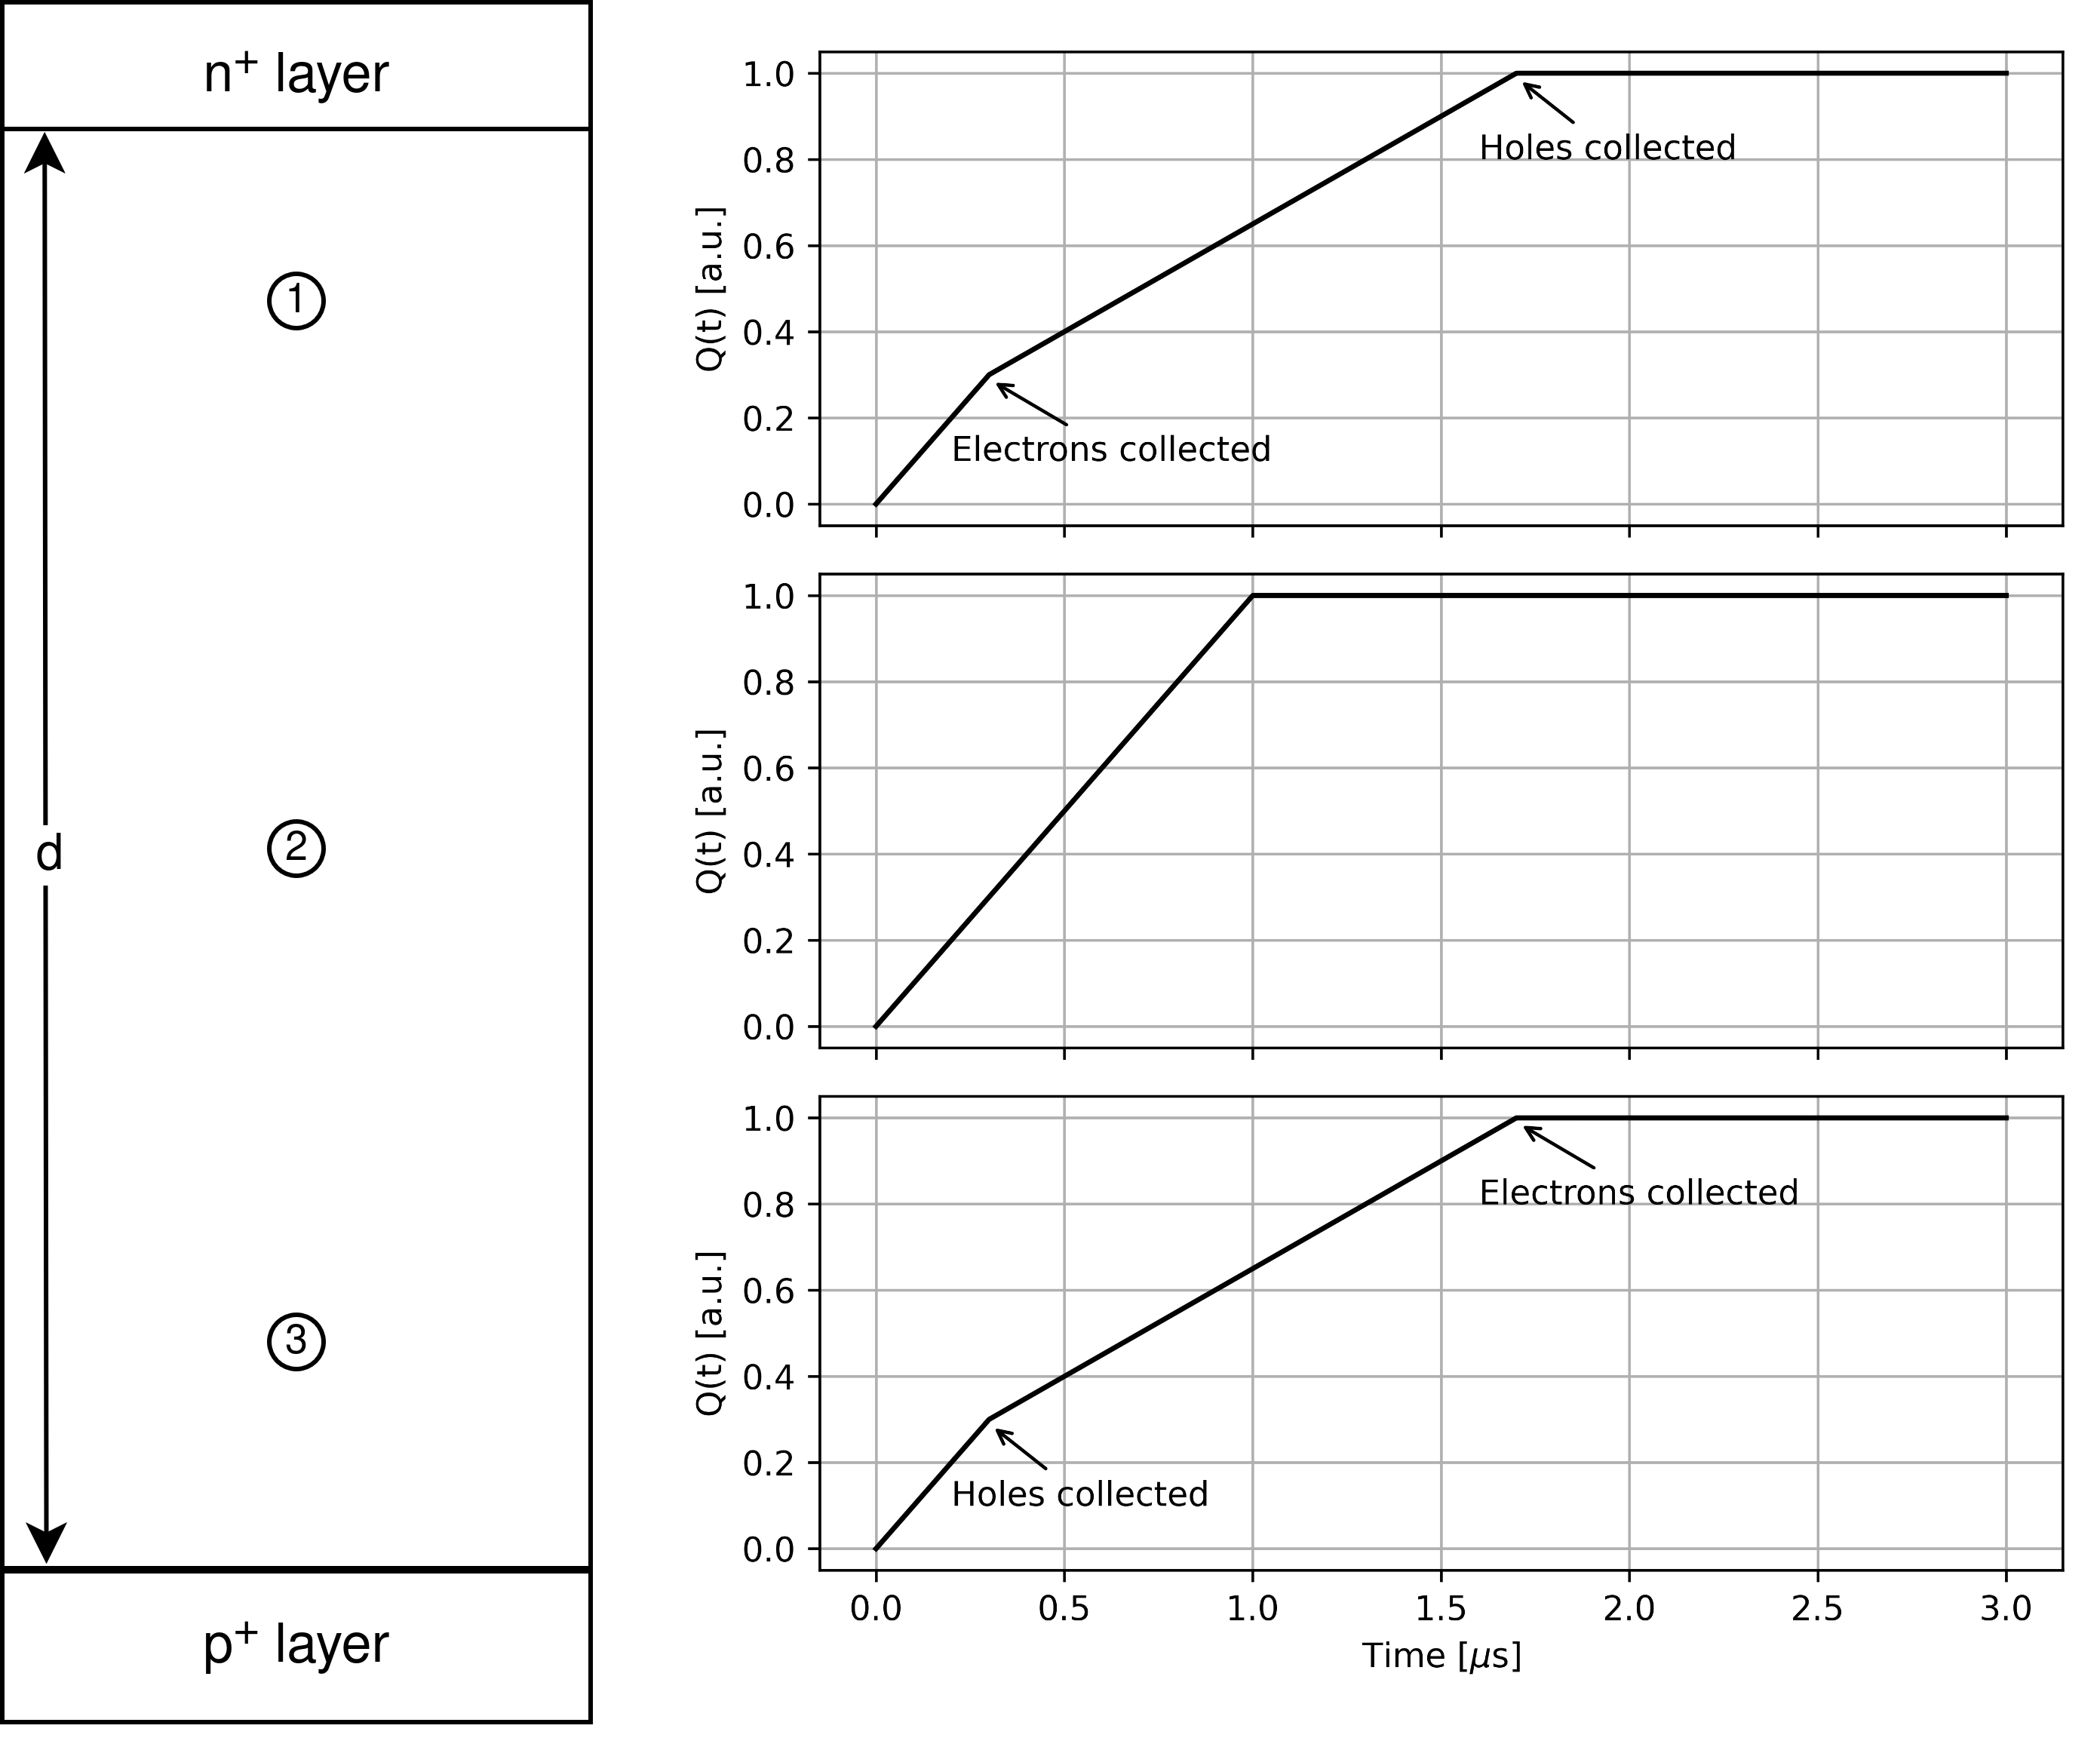
\includegraphics[width=0.85\linewidth]{figures/03_legend/Charge_collection_planar.png}
    \caption{Shape of the leading edge for three energy depositions inside a planar HPGe detector. Charge depositions close to the p$^+$ layer (bottom panel) are characterized by a very fast hole-induced signal, followed by a slower electron-induced signal, as the latter must drift across the entire detector volume. Similarly, charge depositions close to the n$^+$ layer are characterized by fast signals from the electrons, followed by a slower hole-induced signal. Here, we assume a detector of height $d=20$~cm and drift velocities of $10^{7}$~cm/s.}
\label{fig:Pulse_shape}
\end{figure}

In practice, however, signals recorded in HPGe detectors deviate from these idealized shapes due to additional effects that smooth out the signal. 
Crystal defects such as vacancies, dislocations, or impurities can locally trap charge carriers during their drift, preventing a fraction of the charge from reaching the electrodes. This reduces the signal amplitude and degrades energy resolution, as a variable amount of charge is lost.
Not all trapped carriers remain trapped permanently. Some are released after a time delay through de-trapping, which partially restores the signal but leads to a longer rise time. Both effects are illustrated in figure~\ref{fig:trapping_detrapping}~\cite{knoll_radiation_2000}. 


\begin{figure}
    \centering
    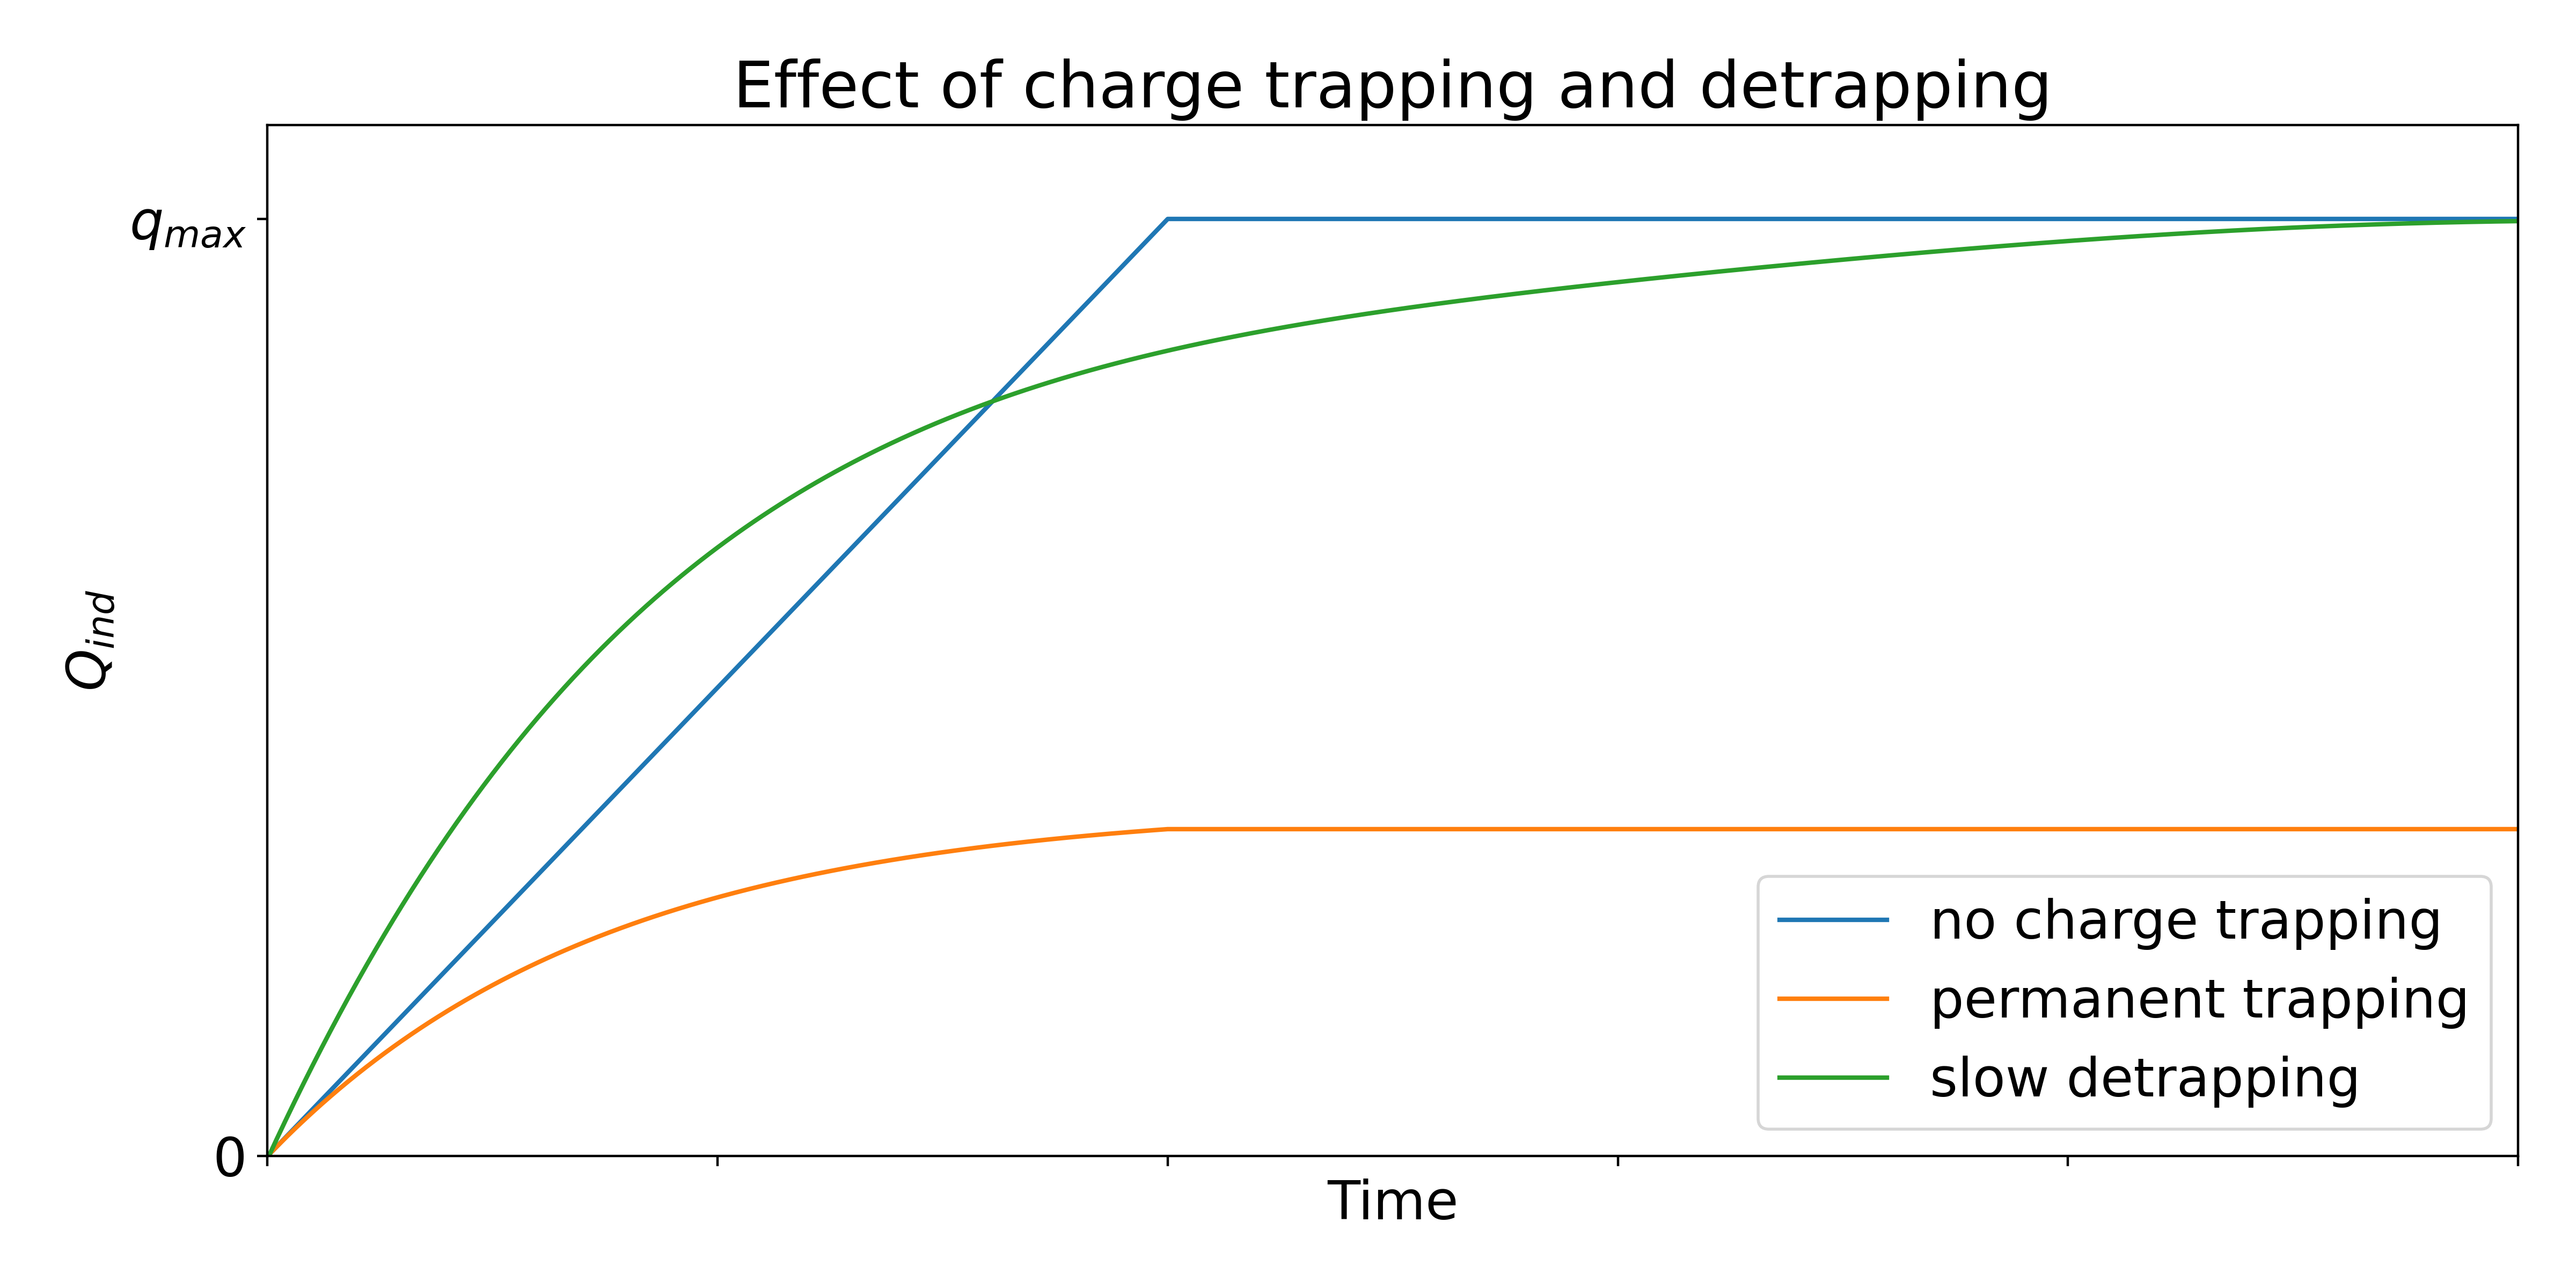
\includegraphics[width=0.75\linewidth]{figures/03_legend/Plot_charge_trapping.png}
    \caption{Effect of charge trapping and de-trapping on the rising edge of a HPGe waveform. Assuming a perfect semiconductor where no charge trapping occurs (blue line), all charges would arrive in a very short period of time, leading to a sharp edge when $q_{\mathrm{max}}$ is reached. On the other hand, permanent trapping would reduce the maximum amplitude. The combined effect of trapping and detrapping results in a smoothed waveform that rises quickly at first, then more slowly over time. For simplicity, only one type of charge carrier is shown. Adapted from~\cite{knoll_radiation_2000}.}
\label{fig:trapping_detrapping}
\end{figure}

Other physical effects further modify the waveform in similar ways: 
Self-repulsion and diffusion cause the charge carriers to spread out into a charge cloud, rather than moving as point-like. As a result, not all charges arrive at the electrode simultaneously, and the sharp edge at $q_{\mathrm{max}}$ becomes smoothed out.
Crystal anisotropy leads to non-uniform drift velocities, since the mobility of charge carriers depends on the orientation of the crystal axes. Table~\ref{tab:charge_mobility} shows electron and hole mobilities for different crystallographic axes, indicated by Miller indices. The charge carrier drift velocity $v_{e/h}$ is related to the mobility as:

\begin{equation}
\label{eq:velocity_mobility}
    v_{e/h} = \mu_{e/h} \cdot E \,,
\end{equation}

\noindent where the subscript indicates electrons and holes, respectively.

\begin{table}
\centering
\caption{Electron and hole mobilities for different crystal axes in germanium at 77~K. The axes are indicated by Miller indices~\cite{Abt_2023}.} 
\label{tab:charge_mobility}
\begin{tabular}{|c | c | c |}
	\hline
    \textbf{Crystal axis} & \textbf{$\mu_e$ [cm$^2$/(Vs)]} & \textbf{$\mu_h$ [cm$^2$/(Vs)]} \\
    \hline
    $\langle100\rangle$ & 38609 & 61824 \\
    \hline
    $\langle111\rangle$ & 38536  & 61215 \\ 
    \hline
\end{tabular}
\end{table}


\subsubsection{HPGe detectors in LEGEND-200}
\label{sec:HPGe_legend}
The LEGEND-200 experiment initially employed the majority of the enriched HPGe detectors that were previously manufactured, characterized, and operated in the GERDA and MJD experiments. GERDA primarily used broad energy germanium (BEGe) detectors, while MJD mainly used p-type point contact (PPC) detectors, where the main germanium crystal is p-doped. Both detector types are optimized for $0 \nu \beta \beta$ decay searches, offering excellent energy resolution, low background levels, and precise event reconstruction capabilities~\cite{collaboration_legend-1000_2021}. 
In later phases of both experiments, a new type of detector was introduced. The p-type inverted coaxial point contact (ICPC) detector allows for larger individual detector sizes while simultaneously increasing the pulse shape discrimination and energy resolution. Typical masses for these types are 1~kg for PPC, 0.7~kg for BEGe and 2-4~kg for ICPC detectors. 
For LEGEND-200, new ICPC detectors were developed and installed. Using larger detectors provides multiple advantages. Most importantly, it reduces the number of required cables, readout electronics, and mechanical support structures, all of which contribute to the overall background. 
Furthermore, a lower surface-to-volume ratio reduces the detector's sensitivity to surface-related backgrounds~\cite{collaboration_legend-1000_2021}. 

Traditional coaxial detectors, which were used in GERDA and have been installed in LEGEND-200 as well, do not offer the same level of performance as ICPC detectors. Consequently, they are not planned for use in future phases of LEGEND. In fact, the LEGEND collaboration will primarily rely on ICPC detectors moving forward. 
Figure~\ref{fig:legend_hpge_types} illustrates the three detector geometries. The layout of the LEGEND-200 detector array, as it was at the point of this work, is shown in figure~\ref{fig:legend_hpge_array}. 


\begin{figure}
    \centering
    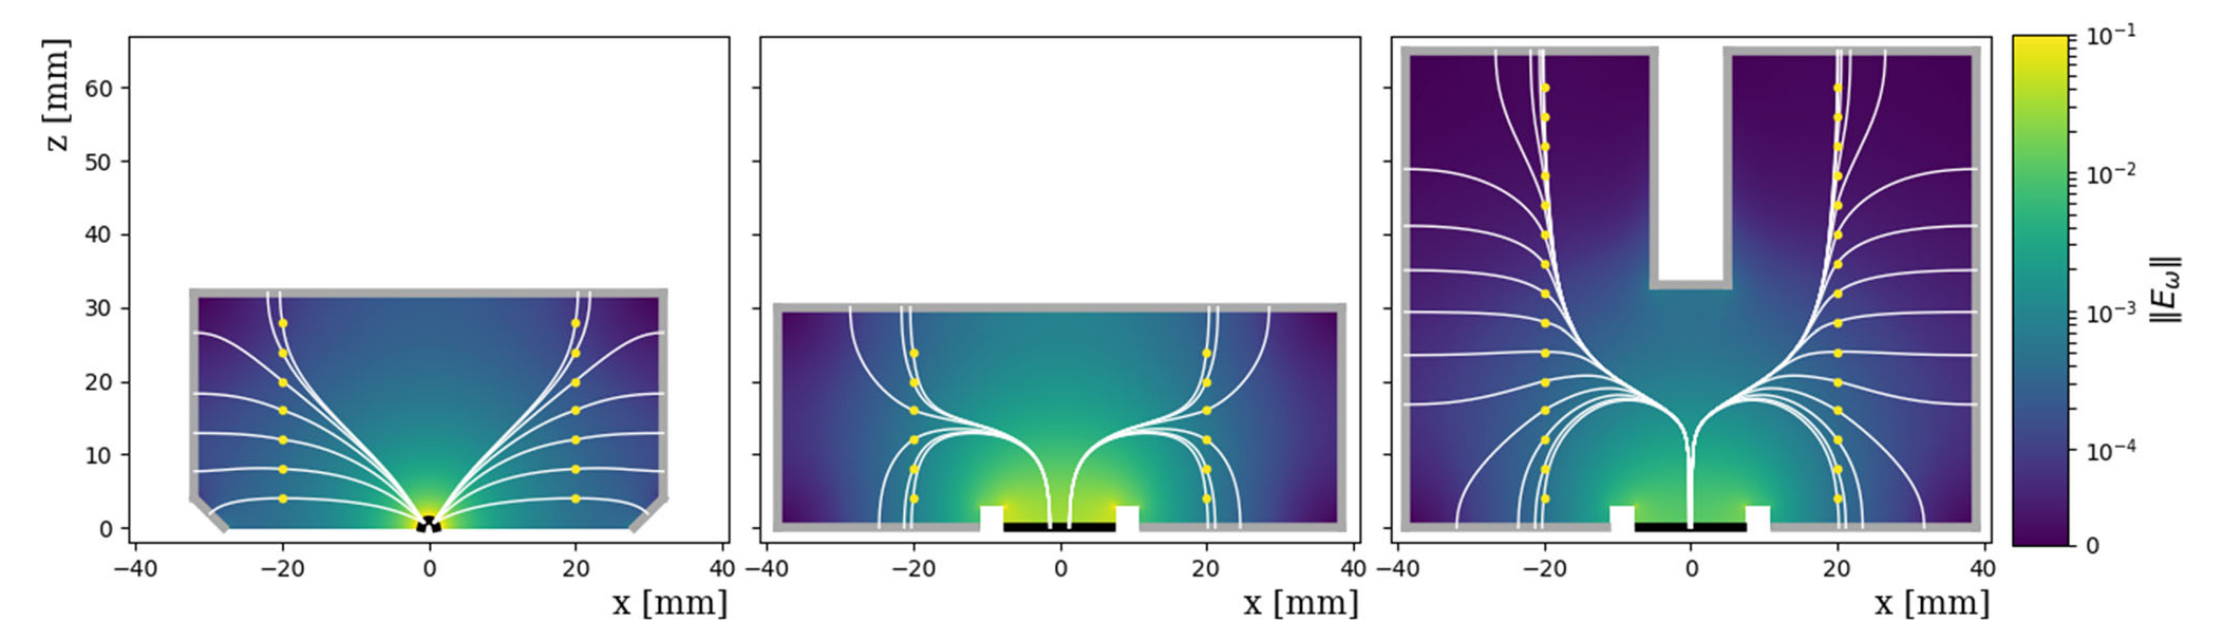
\includegraphics[width=1\linewidth]{figures/03_legend/Detectors_LEGEND.png}
    \caption{Cross section of three detector geometries used in LEGEND-200, including their respective weighting fields: PPC (left), BEGe (middle), and ICPC (right). The black line at the bottom indicates the p$^+$ contact, and the grey line surrounding the detector represents the n$^+$ electrode. Yellow dots mark exemplary interaction points, and white lines show the corresponding charge carrier trajectories. Plot from~\cite{collaboration_legend-1000_2021}.}
    \label{fig:legend_hpge_types}
\end{figure}



\begin{figure}[t]
    \centering
    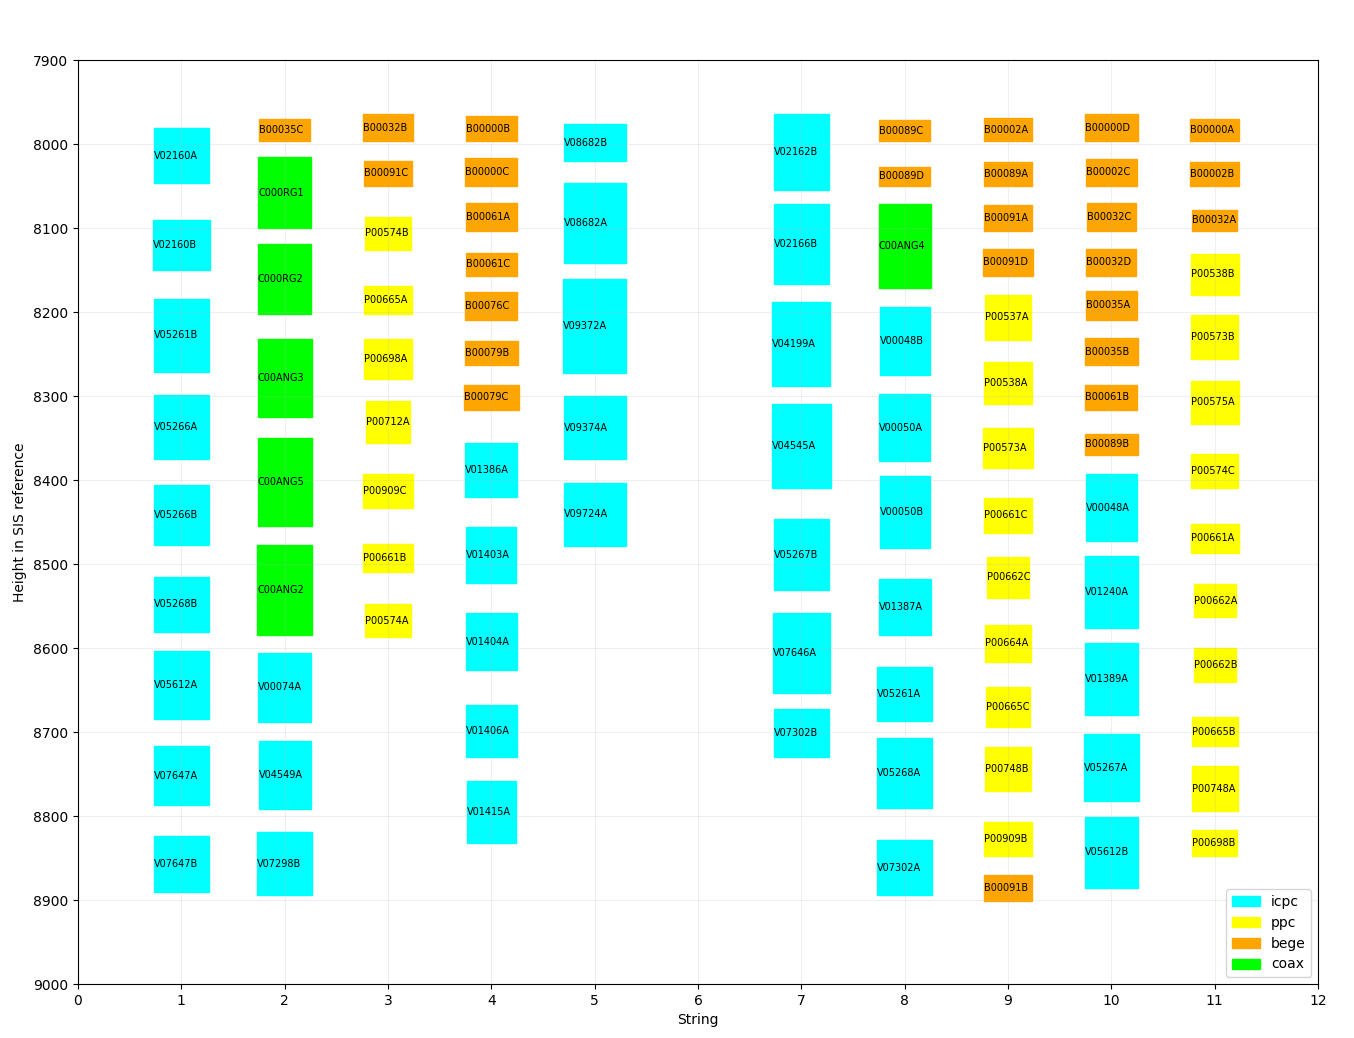
\includegraphics[width=0.95\linewidth]{figures/03_legend/improved_detector_arrangement_SGaelli.png}
    \caption{Detector map of the HPGe array installed in LEGEND-200. The germanium diodes are mounted on 11 strings. The y-axis indicates the vertical position relative to the top of the detector, where the source insertion system is located. The colors indicate the different detector geometries. ICPC detectors are blue, PPC detectors are yellow, BEGe detectors are orange and the coaxial detectors are indicated in green. Image credits of Sandro Gaelli.}
    \label{fig:legend_hpge_array}
\end{figure}



The detectors used in LEGEND-200 are all p-type HPGe diodes, equipped with a relatively thin ($\sim$ 300~nm) p$^+$ electrode that is formed via boron implantation. The n$^+$ electrode, doped with lithium, is significantly thicker ($\sim$ 1-2~mm) and covers most of the detector surface~\cite{agostini_pulse_2022}. The signal is read out from the small p$^+$ electrode, because the charge signal is dominated by hole drift in this geometry. 

In LEGEND-200, detector signals are processed by a two-stage resistive-feedback charge-sensitive amplifier (CSA) operated in liquid argon for cooling and radiopurity. 
The Low-Mass Front End is mounted only millimeters from each HPGe detector, using ultra-radiopure materials and a high-value amorphous-germanium feedback resistor. A differential amplifier, positioned 30–150 cm away, boosts the signal for transmission to the data acquisition (DAQ) system. This design achieves electronic noise equivalent to $< 1$~keV FWHM, energy resolution of $\leq 2.5$~keV at $Q_{\beta \beta}$, and fast ($\leq 100$~ns) rise times, enabling precise energy reconstruction and effective pulse-shape discrimination~\cite{Willers_2020}.

The DAQ system reads out the signals at a rate of 62.5~MHz, corresponding to a sampling interval of 16~ns. This is sufficiently fast to resolve the characteristic signal rise times. The digitized waveform is a voltage step with an exponential decay from the feedback circuit and superimposed electronic noise, and therefore requires further processing.

The digital processing begins with a baseline subtraction and pole-zero cancellation to remove the exponential decay, yielding an idealized step. The resulting waveform is then step-like. The signal is then shaped using a trapezoidal (trap) filter, implemented by subtracting two moving averages of different widths to produce a waveform with a defined rise, flat top, and fall. The flat top is rounded via additional moving averages to yield a single, well-defined maximum. The amplitude is taken as this maximum, and its value is proportional to the collected charge~\cite{Willers_2020, salathe_2016150}.  


\subsection{Calibration of the LEGEND-200 experiment}

A successful search for $0 \nu \beta \beta$ decay requires excellent energy resolution and a stable energy scale, which in turn requires regular calibration of every detector.
After digital signal processing, the waveform remains in units of ADC counts. To convert these into physical energy, radioactive sources with a well-known $\gamma$ spectrum are periodically inserted into the cryostat using an automated source insertion system (SIS). This is necessary because the isotope used for LEGEND-200, as well as GERDA and MJD, $^{228}$Th, has a relatively short half-life of 1.9~years~\cite{collaboration_legend-1000_2021}.
The SIS allows sources to be inserted for calibration runs and removed during physics data-taking. Sources are guided near the detector strings through dedicated copper funnels, which are required to navigate the sources to their calibration positions next to the detectors. LEGEND-200 comprises four SIS, each accommodating four sources~\cite{mueller2023}. 

Once sufficient statistics are collected, the resulting $\gamma$ lines appear in the energy histogram; matching their known energies to the measured ADC positions yields the calibration curve. 
In addition to determining the absolute energy scale, calibration is essential for evaluating the detector's energy resolution. This is critical for $0 \nu \beta \beta$ searches, as a precise determination of the peak at $Q_{\beta \beta}$ with a high resolution is necessary for effective background discrimination and therefore maximizing signal sensitivity.  

$^{228}$Th decays through a series of $\alpha$ and $\beta$ transitions to $^{208}$Pb, emitting several characteristic $\gamma$ rays along the way~\cite{baudis_calibration_2023}. The decay scheme is shown in figure~\ref{fig:Th228_decay_chain}. 

\begin{figure}
    \centering
    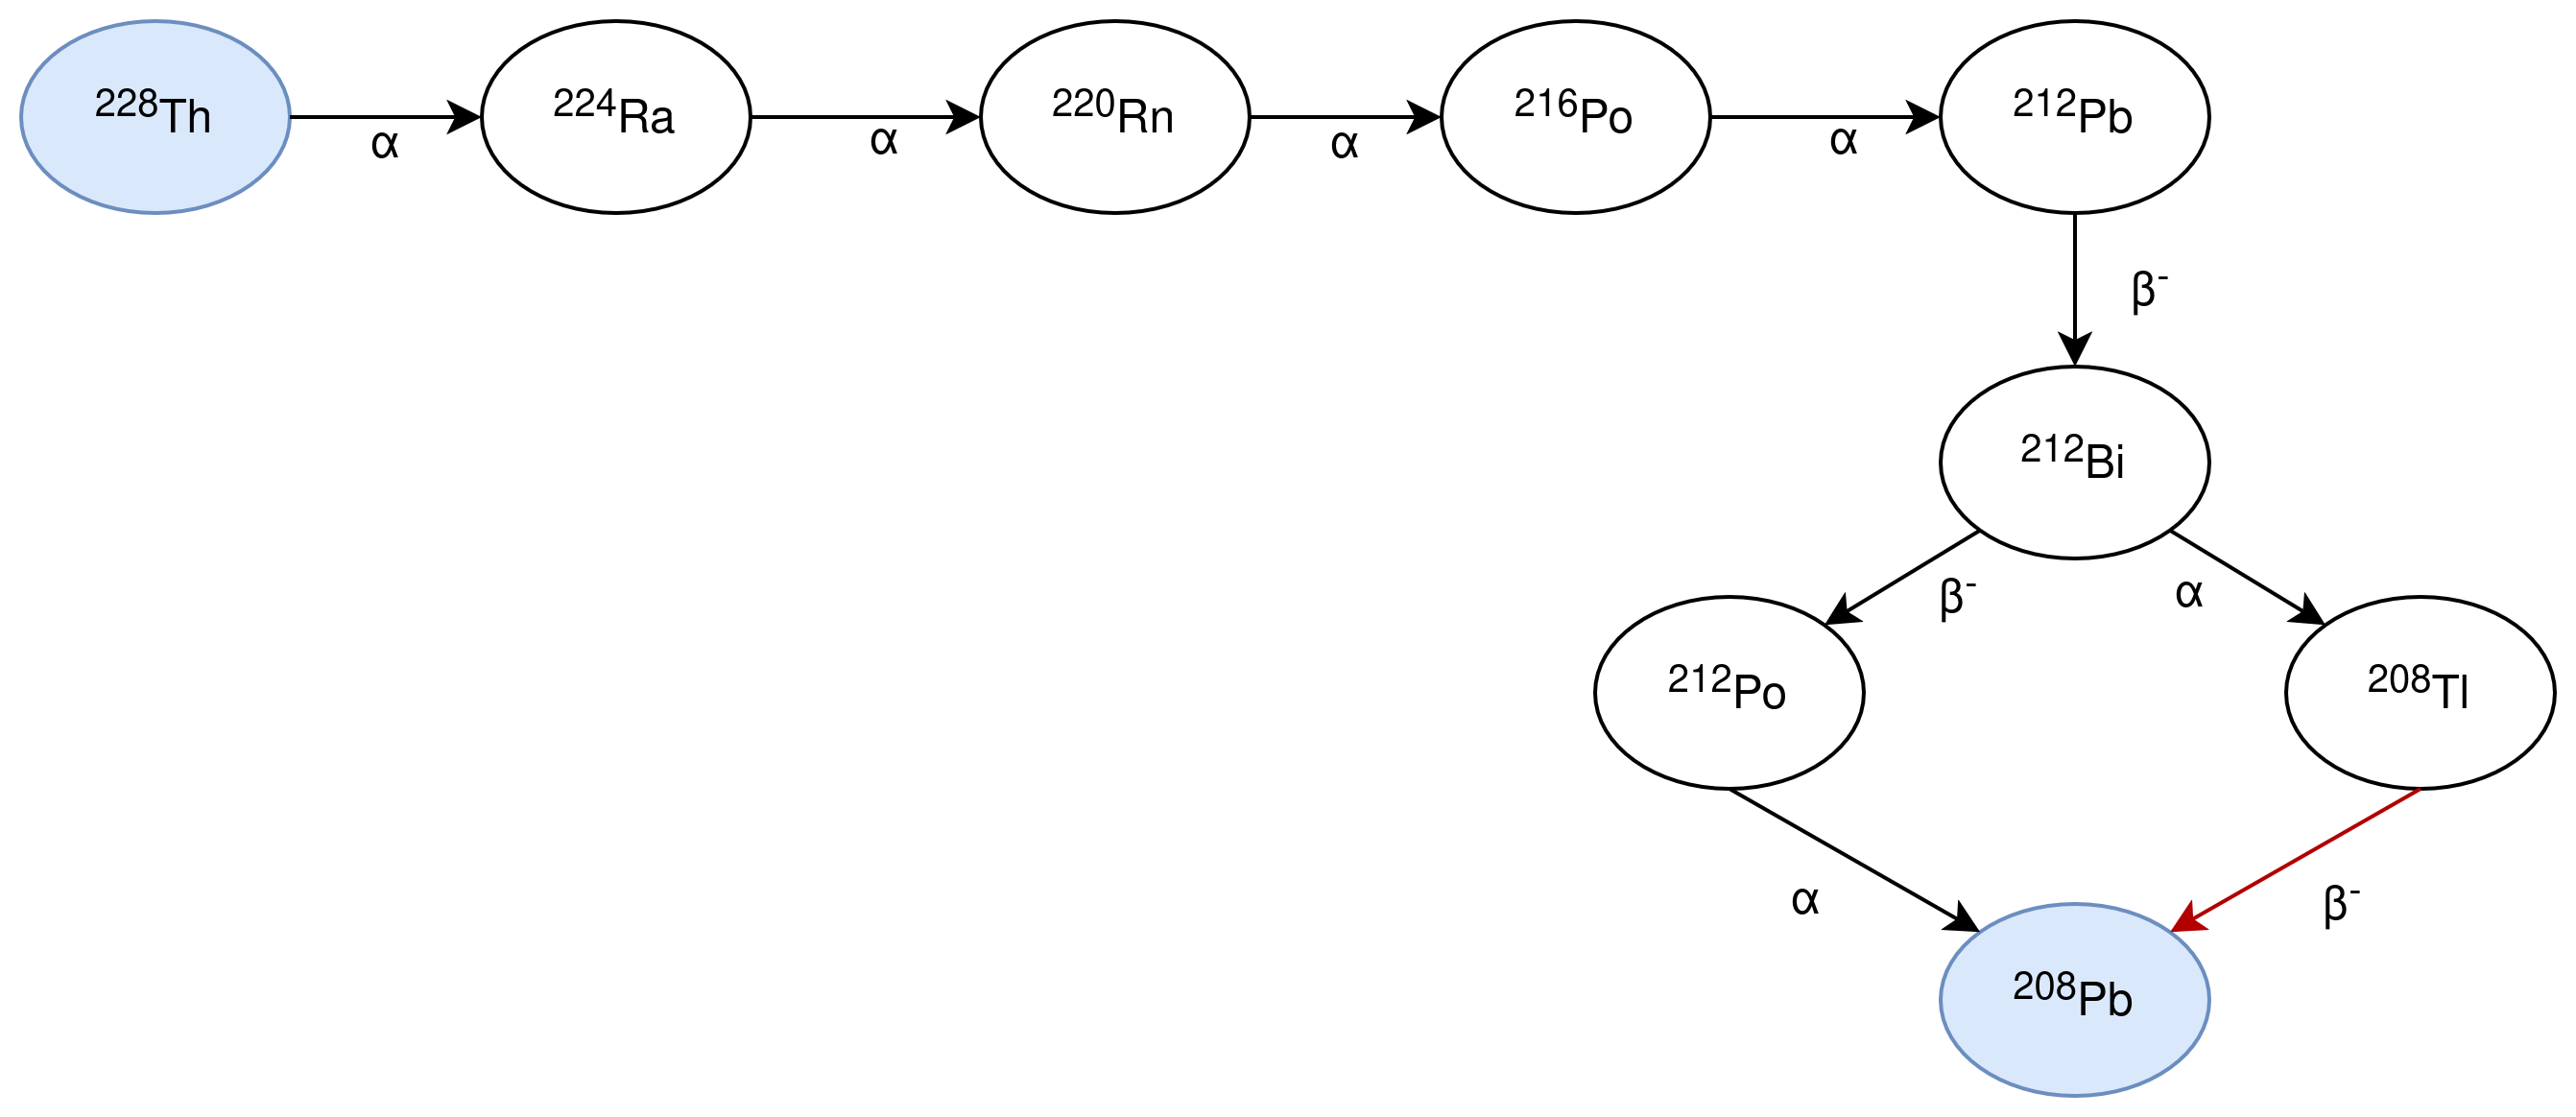
\includegraphics[width=\linewidth]{figures/03_legend/Th228_decay_chain.png}
    \caption{Decay chain of $^{228}$Th to $^{208}$Pb. For energy calibration and pulse shape studies, the $\beta^-$ decay of $^{208}$Tl is most important, because it produces several $\gamma$ lines used for calibration. This decay is indicated by the red arrow.}
    \label{fig:Th228_decay_chain}
\end{figure}

The most important line is the $^{208}$Tl 2614.5 keV $\gamma$. When this photon undergoes pair production inside a HPGe detector, the resulting electron deposits its kinetic energy, and the positron annihilates into two 511 keV photons. Depending on whether none, one, or both annihilation photons escape, three distinct peaks appear: 

\noindent \textbf{Full-energy peak} (2614.5 keV): No photons escape, and the waveform contains multiple events. 

\noindent \textbf{Single-escape peak} (2103.5 keV): One photon escapes, there are still multiple events per waveform due to the time separation between deposits. 

\noindent \textbf{Double-escape peak} (1592.5 keV): Both photons escape, and the remaining energy deposition is highly localized and thus single-site~\cite{baudis_calibration_2023, agostini_pulse_2022}.

A further useful line is the $^{212}$Bi full-energy peak at 1621 keV. Its proximity to the double-escape peak makes it convenient for energy-independent comparisons of single-site and multi-site populations~\cite{agostini_pulse_2022}. Figure~\ref{fig:Calibration_spectrum_Th228} shows a representative $^{228}$Th calibration spectrum recorded with a single ICPC detector in LEGEND-200, with the key peaks highlighted.   


\begin{figure}
    \centering
    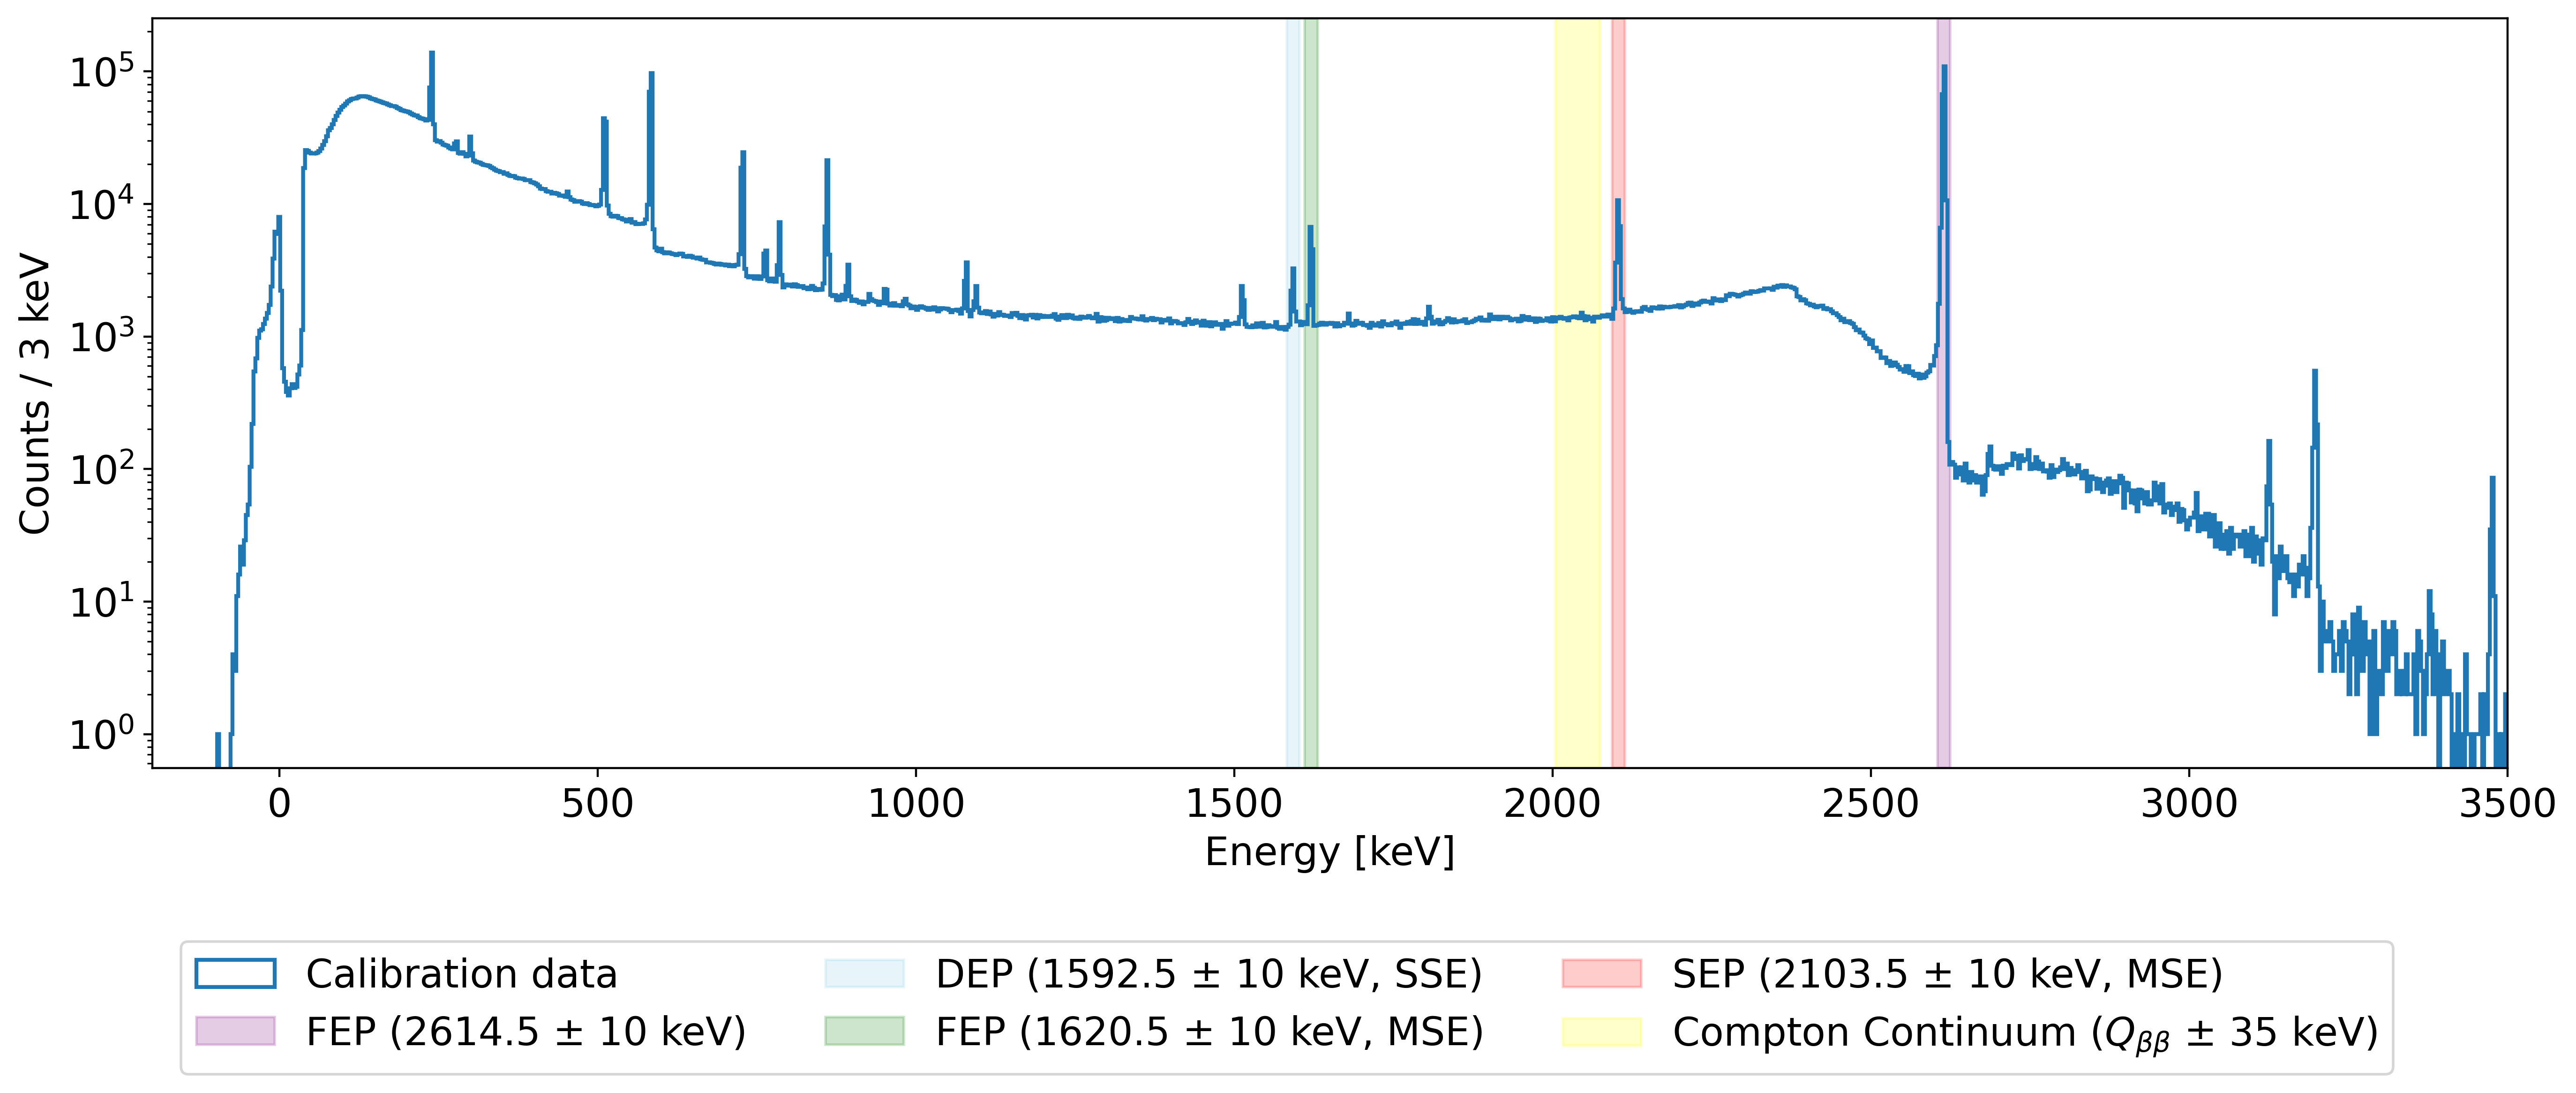
\includegraphics[width=\linewidth]{figures/03_legend/Calibration_spectrum_Th228_V09372A.png}
    \caption{Energy spectrum from a $^{228}$Th calibration run (period 9, run 3) in LEGEND-200. The spectrum corresponds to a single IC detector (V09372A) and a 5-hour data acquisition. Prominent $\gamma$-ray lines used for calibration and PSD studies are indicated.}
    \label{fig:Calibration_spectrum_Th228}
\end{figure}


In addition to $^{228}$Th, LEGEND also recorded data with a $^{56}$Co source. It is not used for detector calibration, but since it emits several $\gamma$ lines at energies that complement those of $^{228}$Th, it is a valuable source for studying the energy dependence of the PSD efficiency. 


\subsection{Background rejection: pulse shape discrimination}
\label{sec:02_PSD}

Even with large detector masses and multi-year exposures, only a handful of $0 \nu \beta \beta$ decay events are to be expected. At the same time, numerous background processes can deposit energy in the region of interest around $Q_{\beta \beta} = 2039$~keV.
Without effective background rejection methods, these events would obscure the $0\nu\beta\beta$ signal entirely. Moreover, as shown in equation~\refeq{eq:0vbb_hl_sensitivity}, the experimental sensitivity to the half-life scales inversely with the square root of the background index, meaning that lowering the background significantly improves sensitivity. 
Background rejection in LEGEND is achieved through a combination of material selection, active veto systems, and signal-based analysis techniques. Of particular importance for this work is pulse shape discrimination, which is possible because HPGe detectors record ionization signals with high temporal and spatial precision.
In LEGEND, we distinguish between four characteristic pulse shapes: 


\textbf{Single-site events (SSE)} are characterized by very localized energy depositions. This applies to both $0 \nu \beta \beta$ and $2 \nu \beta \beta$ decays, where the electrons deposit their energy within a small volume (typically $\sim 1$~mm$^3$). The resulting charges drift to the electrodes nearly simultaneously, and the waveform resembles that of a single interaction.

\textbf{Multi-site events (MSE)} involve energy deposited at multiple locations, typically due to multiple Compton scatterings of high-energy $\gamma$ rays from natural radioactivity. These events are classified as background in the context of neutrinoless double beta decay. 

Surface events occur near the detector boundaries and are also associated with the background. \textbf{P-contact events}, such as $\alpha$ interactions near the p$^{+}$ electrode, produce a fast-rising signal, since the drift path is short. Such surface events are particularly dangerous because their localized energy deposition can mimic the topology of SSEs, but their distorted charge collection leads to subtle differences in the pulse shape that must be carefully identified and rejected. 
In contrast, \textbf{n-contact events}, which originate near the $n^{+}$ electrode, involve long drift paths for the holes through the entire detector. These signals tend to rise more slowly and may show distortions due to trapping, de-trapping, or charge loss in the dead layer.


\begin{figure}[t]
    \centering
    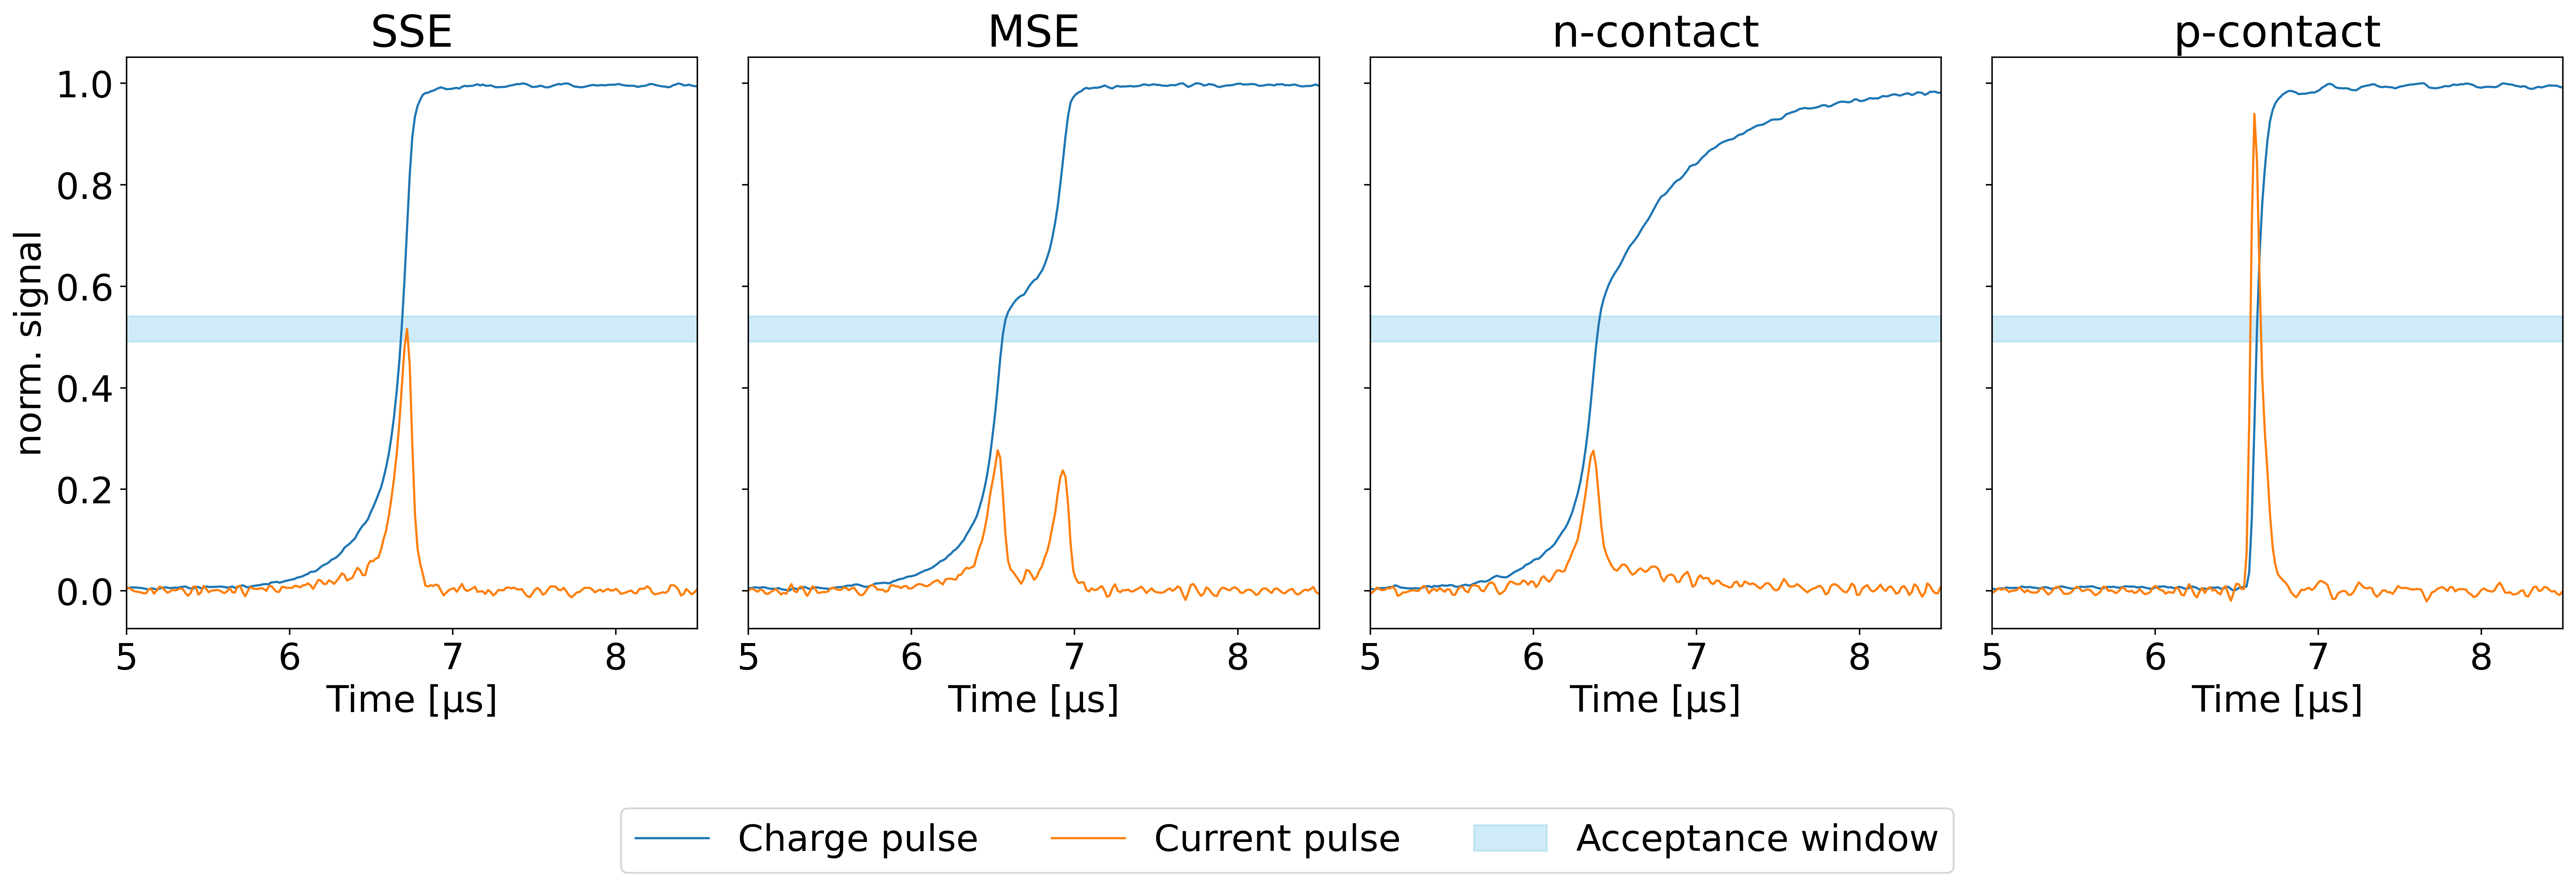
\includegraphics[width=\linewidth]{figures/03_legend/PSD_topology.png}
    \caption{Example waveforms from a $^{228}$Th calibration run in LEGEND-200, showing the normalized induced charge and corresponding current signal for four different event types. All examples have the same total deposited energy. The blue band illustrates, schematically, the A/E acceptance window for SSE-like signals; it is not derived from a quantitative cut but serves to illustrate the idea.}
    \label{fig:PSD_topology}
\end{figure}

Figure~\ref{fig:PSD_topology} illustrates these event types.
The standard PSD parameter is the amplitude over energy ratio (A/E), also referred to as AoE. Here, $A$ denotes the maximum of the waveform and $E$ is the reconstructed event energy, expressed in~keV after energy calibration. The A/E parameter is sensitive to the event topology: in SSE, all the energy is deposited in a localized volume, leading to a short charge collection time and thus a sharply peaked current pulse. In MSE, the energy is deposited in several locations, resulting in less peaked current pulses and smaller A/E ratios. 

The A/E distribution is calibrated by performing peak fits on $^{228}$Th calibration data. In the Compton bands, the A/E distribution is characterized by a Gaussian single-site band with a low-side tail from MSE and $n^{+}$ surface events. A high-energy tail accounts for $p^{+}$ surface events. The tails are modelled as an exponential distribution convolved with a Gaussian. 

Two corrections are applied. The A/E parameter depends on the drift time and the energy. Charge clouds drifting through the detector are subject to diffusion, which broadens the current signal. The A/E energy dependence is modelled as:

\begin{align}
\label{eq:AoE_energydep_mu}
\mu_{\mathrm{A/E}}(E) & = a + b \cdot E \\
\sigma_{\mathrm{A/E}}(E) & = \sqrt{c + \frac{d}{E^2}}
\label{eq:AoE_energydep_sigma} \,,
\end{align}

\noindent where $a,b,c,d$ are determined from calibration data in the Compton region from 900~keV to 2300~keV.  
For uniformity across detectors and calibration periods, a normalized A/E classifier is defined:


\begin{equation}
\label{eq:AoE_Classifier}
A/E_{\mathrm{classifier}} = \frac{\frac{A/E}{\mu_{A/E}(E) - 1}}{\sigma_{A/E}(E)} \,.
\end{equation}

This normalization accounts for detector-specific and time-dependent variations in the A/E response, enabling a unified classifier scale that allows consistent pulse shape discrimination across all detectors and calibration periods~\cite{lnote_24013}.


To isolate single-site events, two cut values are applied. 
The lower cut, which removes multi-site and n-contact events, is chosen such that 90\% of events in the $^{208}$Tl DEP survive. The upper cut is fixed to exclude high-amplitude surface events, in particular, $\alpha$ interactions~\cite{agostini_pulse_2022}.

The Late Charge (LQ) is a PSD parameter that measures the slowness of the final 20\% of charge carriers for an event. It is defined as the area above the rising edge of the waveform after it reaches 80\% of its maximum value. It is a powerful discriminator to identify events with slow charge collection, such as $p^{+}$ contact surface $\alpha$ interactions or events affected by significant charge trapping. 
Like the A/E parameter, the LQ parameter is both drift-time and energy dependent, and needs to be corrected for~\cite{lnote_24013}. 
The A/E and LQ distributions as functions of energy for a single IC detector are shown in figure~\ref{fig:Aoe_LQ_spectra}. 

\begin{figure}
    \centering
    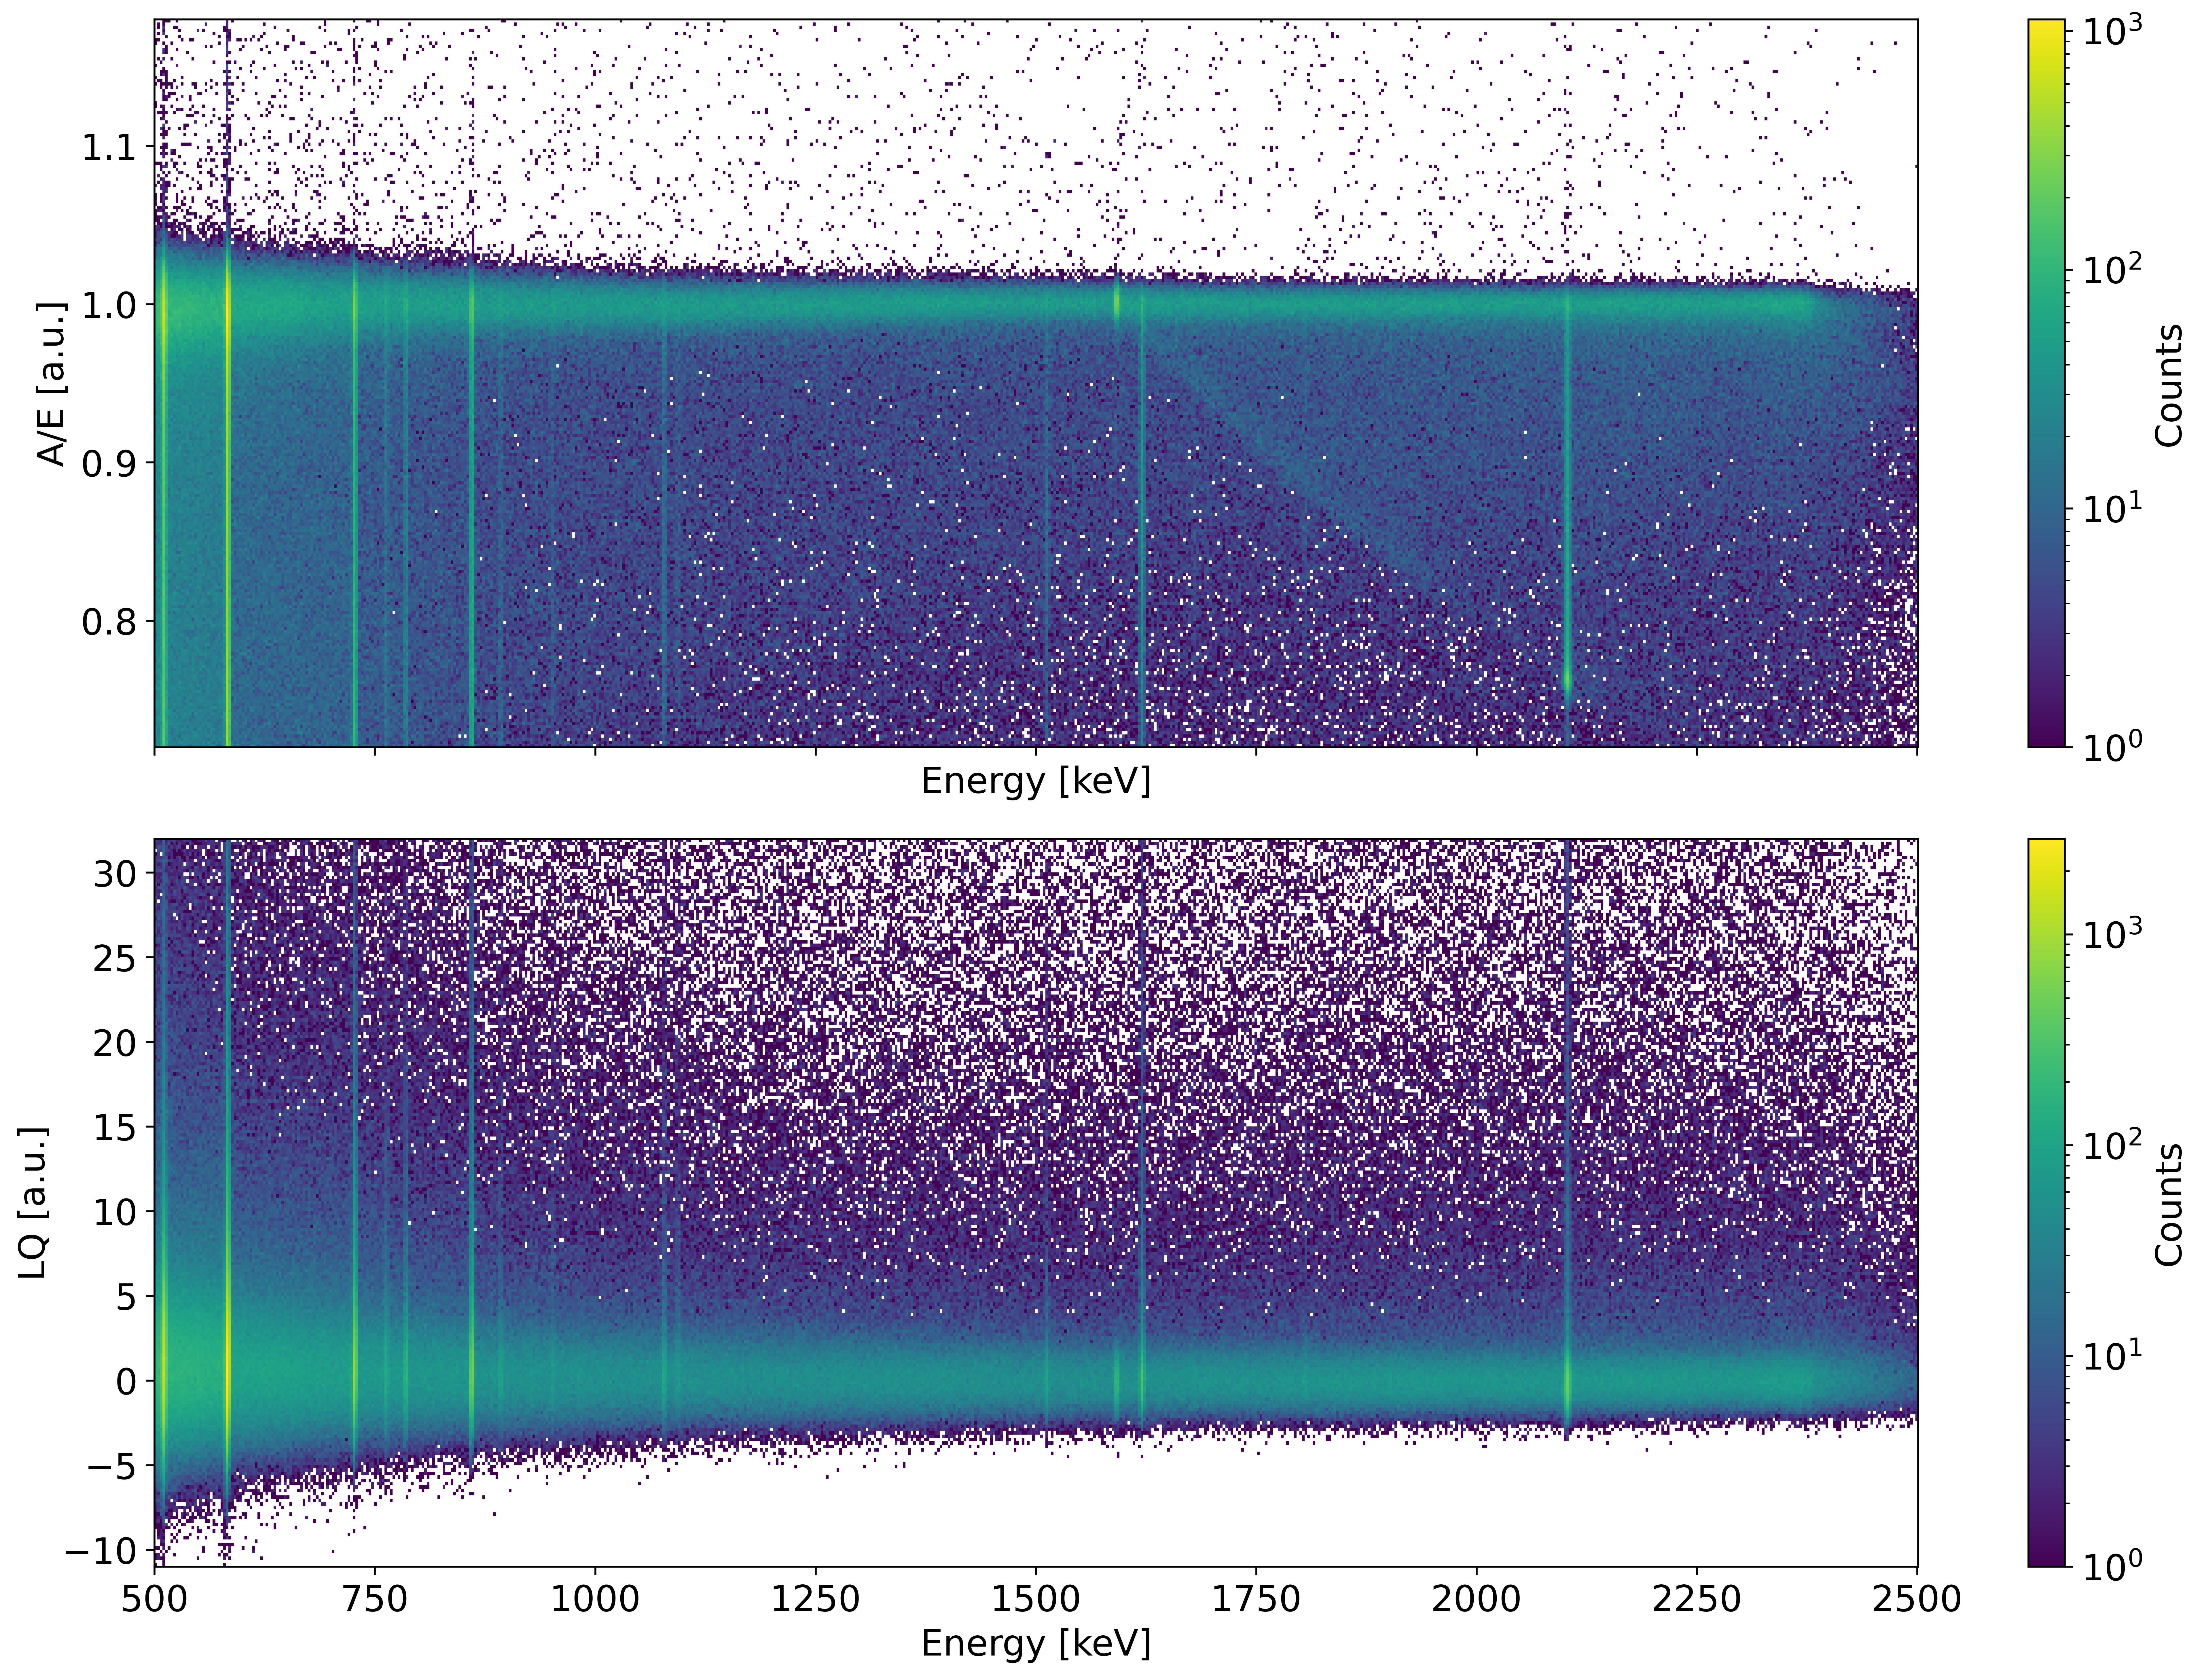
\includegraphics[width=0.85\linewidth]{figures/03_legend/Plot_Aoe_LQ_V09372A.png}
    \caption{Distributions of A/E (top) and LQ (bottom) as a function of energy for the same dataset as in figure~\ref{fig:Calibration_spectrum_Th228} ($^{228}$Th, period 9, run 3, detector V09372A). Both PSD parameters show a narrow single-site band, centered around 1 for A/E and around 0 for LQ, which is successfully corrected for energy dependence. }
    \label{fig:Aoe_LQ_spectra}
\end{figure} 


%--------------------- ML & Transformers ---------------------
\clearpage
\section{Machine learning principles and Transformer architecture} 
\markboth{ML principles and Transformer architecture}{ML principles and Transformer architecture}
\label{sec:04_transformer}

This chapter introduces fundamental concepts of machine learning and deep learning that underpin the waveform classification task addressed in this thesis. It begins with linear regression, a foundational method familiar to most physicists, to illustrate basic supervised learning principles.
Next, the multilayer perceptron (MLP) is presented as a foundational neural network model to introduce core deep learning principles, such as optimization techniques and the backpropagation algorithm. 
Finally, the chapter explores the Transformer architecture, focusing on the encoder component, which is most relevant for waveform classification tasks like those in LEGEND-200. Core components of Transformer networks, such as positional encoding and the attention mechanism are explained, as they are essential for modeling the temporal structure of waveform data. 

\subsection{Machine learning and deep learning}
There is no fixed definition of Artificial Intelligence (AI), but it usually describes systems that simulate intelligent behavior. Machine learning (ML) is a subfield of AI concerned with constructing mathematical models that learn patterns from data to perform tasks such as classifying events or estimating continuous quantities~\cite{badillo_introduction_2020, prince_understanding_2023}. 
ML algorithms are commonly grouped into several paradigms. Two of the most widely used are:

a) Unsupervised learning: Only the input data is available, and the goal is to discover structure without labeling targets. Typical techniques are clustering (partitioning data into similar subsets) and dimensionality reduction (compressing data while preserving salient information)~\cite{badillo_introduction_2020}. 

b) Supervised learning: Models learn a mapping $f(x, \boldsymbol{\theta})$ from inputs $x$ to known targets $y$. If $y$ takes discrete values (e.g., classifying a waveform as signal or background), the problem is one of classification; if $y$ is continuous, it is a regression task~\cite{prince_understanding_2023, badillo_introduction_2020}. 


To illustrate these concepts concretely, consider a one-dimensional linear regression, where the goal is to find a mapping of the form:

\begin{equation}
\label{eq:linear_regression}
	f(x, \boldsymbol{\theta}) =  \theta_0 + \theta_1 \cdot x \,.
\end{equation}

In general, $\theta_0$ is denoted as the bias, and $\theta_1$ is the weight. Simply, the goal is to find the parameter vector $\boldsymbol{\theta}$ that minimizes the discrepancy between the model predictions $f(x, \boldsymbol{\theta})$ and the true outputs $y_i$. A common choice is the sum of squared errors, known as least squares loss:

\begin{equation}
\label{eq:least_squares}
	L[\theta] = \sum_i^N \left( f(x_i, \boldsymbol{\theta}) - y_i \right)^2 \,.
\end{equation}

\noindent Minimizing this loss yields the optimal parameters $\hat{\boldsymbol{\theta}}$ for which the model's predictions best approximate the training data: 

\begin{equation}
\label{eq:optimize_loss_function} 
	\hat{\boldsymbol{\theta}} = \underset{\boldsymbol{\theta}}{\mathrm{argmin}} \; L\left[\boldsymbol{\theta}\right] \,.
\end{equation}

This procedure is referred to as training the model. Once trained, the model can be used to make predictions on new, unseen input data. If the model is too simple to capture the true underlying structure of the data, it is said to be underfitted. Conversely, if the model is excessively complex and learns noise or random fluctuations in the data, it is overfitted and likely to generalize poorly to unseen inputs~\cite{prince_understanding_2023}. 

\subsubsection{Multilayer perceptrons}
\label{sec:03_mlp}

Finding suitable features for machine learning models is often a challenging and time-consuming task. In fact, until recently, progress in machine learning was largely constrained not by model complexity but by the need for effective, manually crafted feature transformations. 
Deep learning (DL) addresses this limitation by integrating the feature transformation step directly into the model itself~\cite{lecun_deep_2015}. Instead of requiring handcrafted input features, DL models learn them automatically from raw data. This is accomplished by introducing additional parameters $\boldsymbol{\vartheta}$ that govern the structure of the feature transform:  

\begin{equation}
\label{eq:dl_feature_transform}
	f(x; \boldsymbol{\theta}, \boldsymbol{\vartheta}) = \theta_0 + \theta_1 \cdot \phi(x; \boldsymbol{\vartheta})\,.
\end{equation}

The key idea is that a recursive composition of simple functions can model highly complex, non-linear mappings. Non-linearity in the functions is essential, as without it, the stacked layers would collapse to a single affine transformation. This is formalized by expressing the overall model as a composition of layers:

\begin{equation}
\label{eq:dl_recursive_feature_transform}
f(\mathbf{x}; \boldsymbol{\theta}) = f_L(f_{L-1}(\ldots f_1(\mathbf{x})) \ldots )) \,.
\end{equation}

where each $f_l$ represents a transformation at layer $l$, which often involves a linear mapping followed by a non-linear activation. The input vector $\mathbf{x}$ is successively transformed through these layers, enabling the network to extract hierarchical features of increasing complexity. Models that follow this idea are referred to as feedforward neural networks, or more specifically, multilayer perceptrons (MLPs)~\cite{lecun_deep_2015, murphy_probabilistic_2022}. 

At the core of these architectures lies the perceptron, a computational unit that performs a weighted sum of its inputs followed by a nonlinear activation. By arranging many such units in layers, MLPs are able to model a wide range of nonlinear functions through learned hierarchical representations. 

\begin{figure}
    \centering
    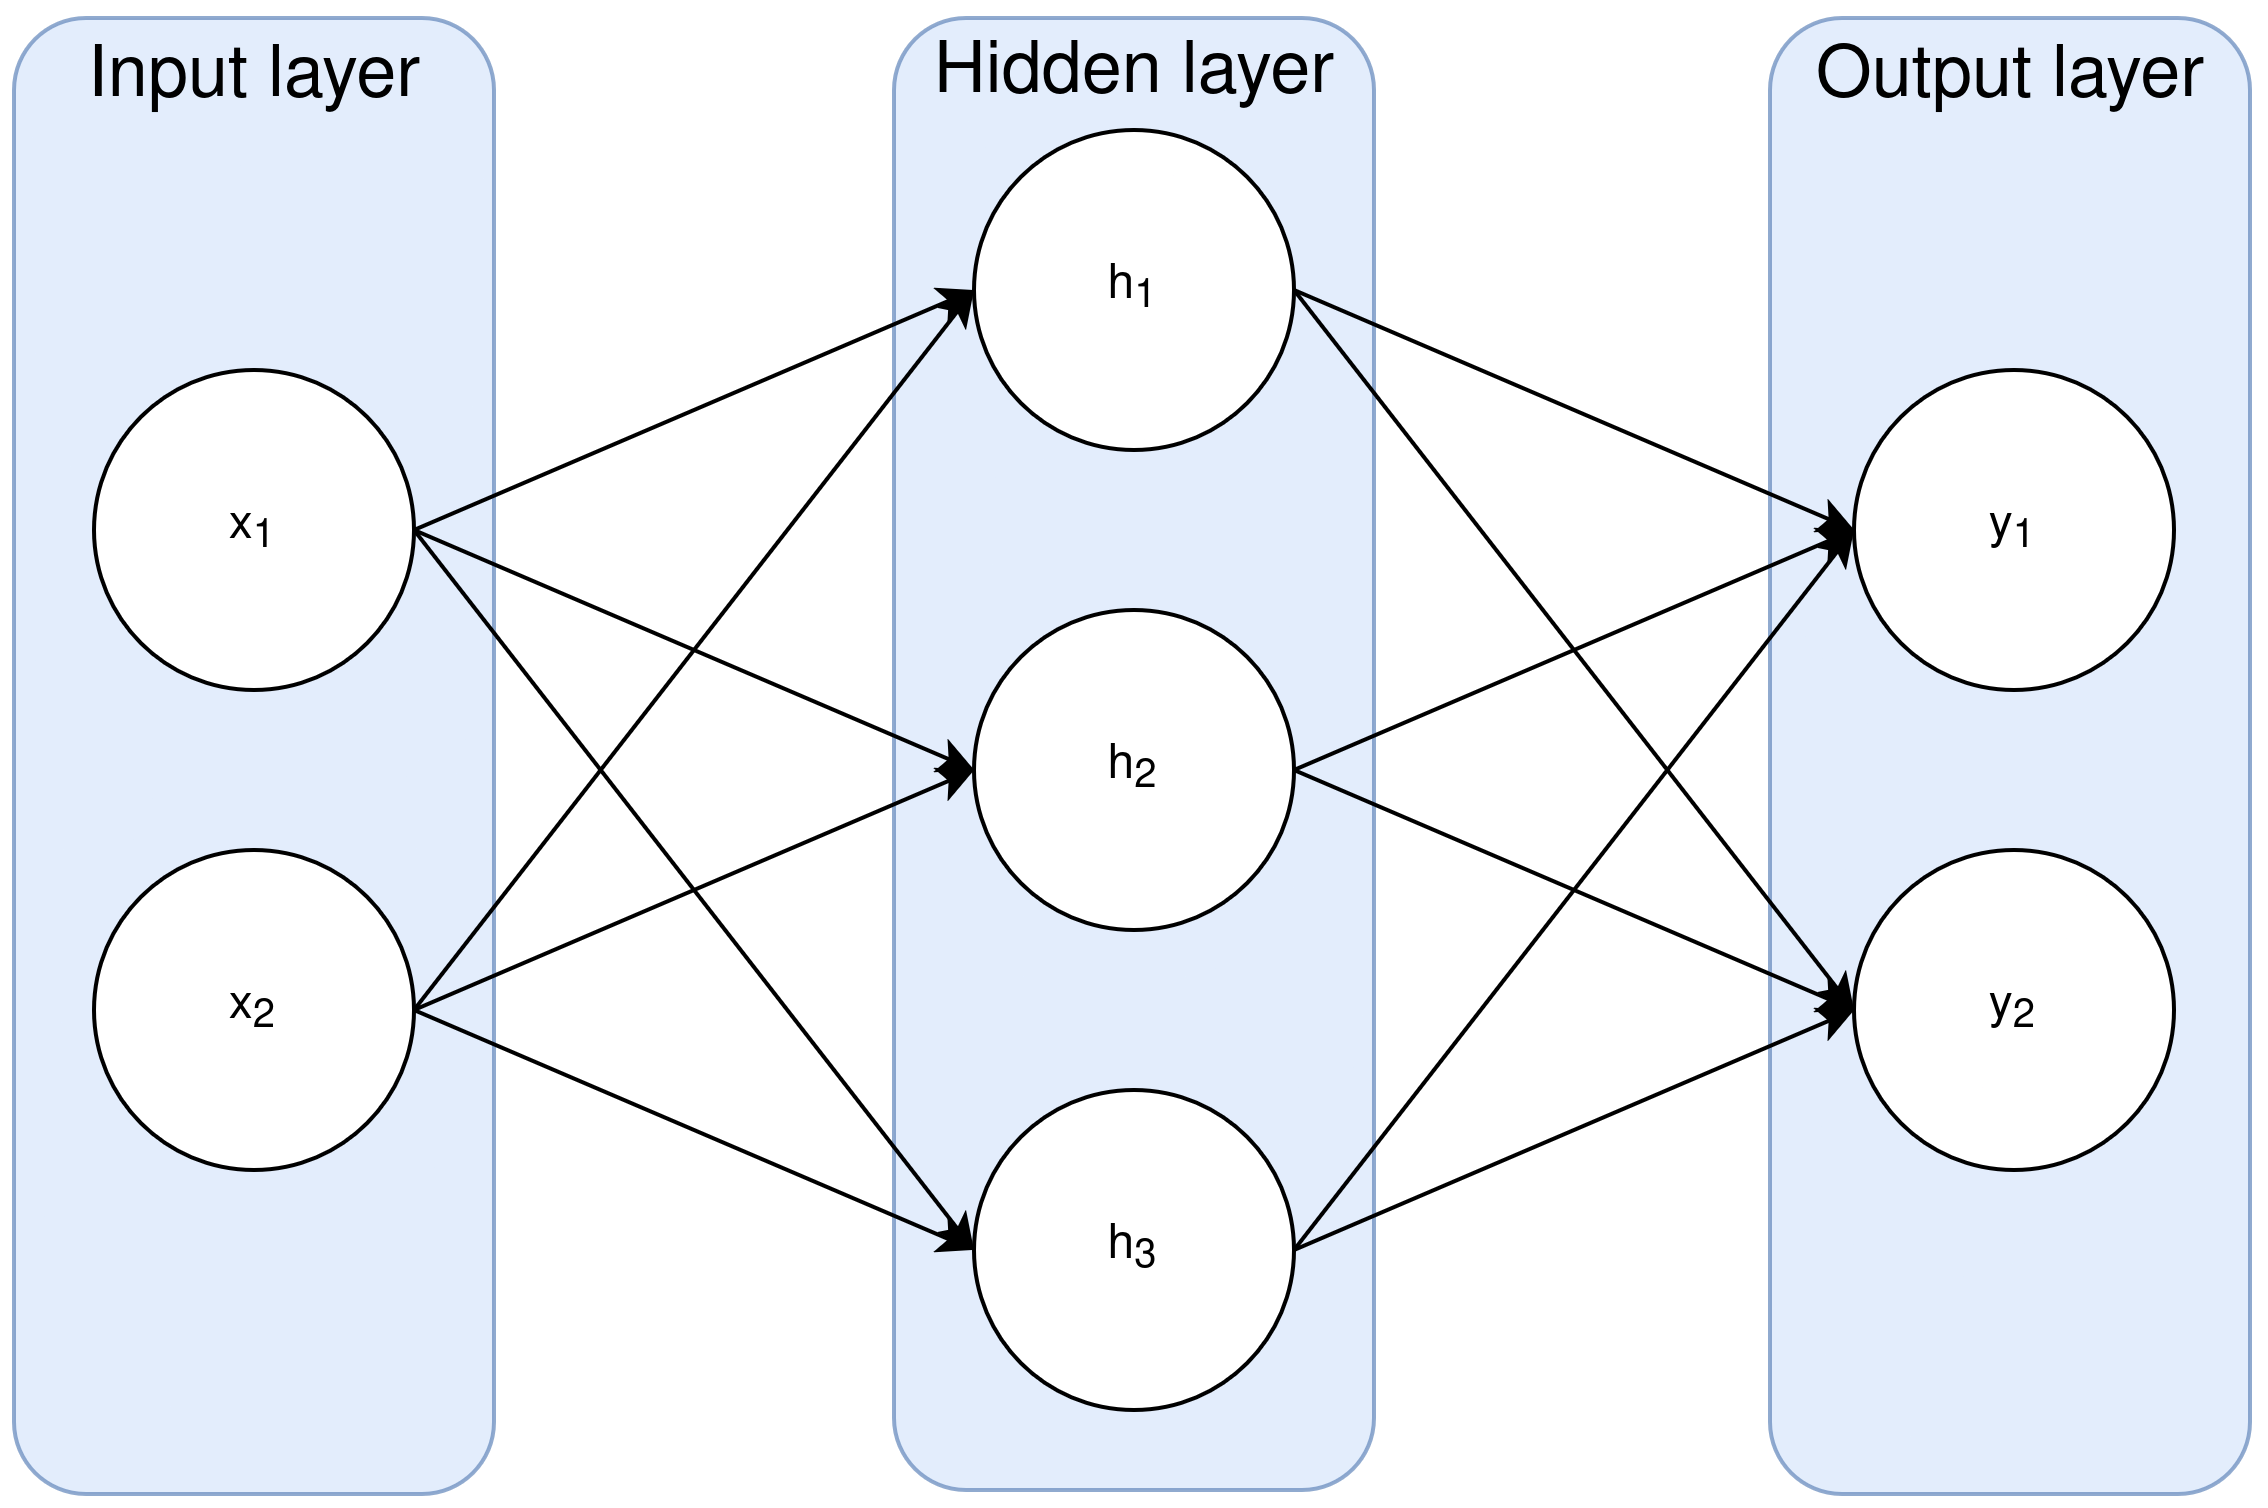
\includegraphics[width=0.6\linewidth]{figures/04_transformer/Shallow_NN.png}
    \caption{Visualization of a feedforward neural network with a single hidden layer containing three neurons, two inputs, and two outputs. The network is fully connected, meaning every unit in one layer is connected to every unit in the next. This is also referred to as a multilayer perceptron. }
\label{fig:shallow_NN}
\end{figure}

Figure~\ref{fig:shallow_NN} shows a shallow feedforward neural network, i.e., one with only a single hidden layer. In a fully connected layer, each neuron is connected to every neuron in the adjacent layers. Although fully connected layers are standard in MLPs, alternative connection patterns exist. 
The first layer is the input layer, the last is the output layer, and all intermediate layers are referred to as hidden layers~\cite{prince_understanding_2023}. In the figure, the hidden layer consists of three computational units, commonly referred to as neurons. 

The computation of a hidden layer is shown in equation~\refeq{eq:NN_hiddenlayer}, where $\mathbf{x} \in \mathbb{R}^d$ is the input vector, $\mathbf{W}_{\theta} \in \mathbb{R}^{m \times d}$ the weight matrix and $\mathbf{b}_{\theta} \in \mathbb{R}^m$ is the bias vector. The non-linear activation function $F$ is applied element-wise. 
The pre-activation (linear part) is given by $\mathbf{W}_{\boldsymbol{\theta}} \cdot \mathbf{x} + \mathbf{b}_{\boldsymbol{\theta}}$, and the activation function transforms it into the hidden representation $\mathbf{h}$. 

An alternative form uses the augmented weight matrix $\mathbf{W'}_{\boldsymbol{\theta}}$ and augmented input $\mathbf{x'}$ to absorb the bias term: 

\begin{align}
\label{eq:NN_hiddenlayer}
	\mathbf{h} & = F \left[ \mathbf{b}_{\theta} + \mathbf{W}_{\theta} \cdot \mathbf{x} \right] = F \left[ \mathbf{W'}_{\theta} \cdot \mathbf{x'} \right] \,,\\
\label{eq:NN_hiddenlayer_out}
	\mathbf{y} & = \mathbf{b}_{\vartheta} + \mathbf{W}_{\vartheta} \cdot \mathbf{h} = \mathbf{W'}_{\vartheta} \cdot \mathbf{h'} \,.
\end{align}

\noindent where $\mathbf{h}$ is the hidden layer. The final output $\mathbf{y}$ is typically a linear transformation of the last hidden layer, optionally followed by an output activation depending on the task. 

While the transformations used in neural networks are commonly referred to as linear layers, they are affine transformations. The inclusion of a bias term makes them not strictly linear in the mathematical sense. However, this can be reformulated as a purely linear operation by augmenting the input vector and weight matrix. Specifically, by extending the input as 

\begin{equation}
\label{eq:affine_to_linear_x}
    \mathbf{x'} = \begin{pmatrix} \mathbf{x} \\ 1 \end{pmatrix} \,,
\end{equation}

\noindent and defining the corresponding augmented weight matrix as

\begin{equation}
\label{eq:affine_to_linear_W}
	\mathbf{W'} = 
	\begin{pmatrix} \mathbf{W} & \mathbf{b}\\
	\mathbf{0}^{\intercal} & 1 \end{pmatrix} \,.
\end{equation}

This trick is widely used in machine learning to streamline notation and implementation, and as such, the bias term is often implied rather than explicitly written. The use of this augmented formulation also clarifies why these layers are often referred to as linear, even though they technically are not. 


\subsubsection{Activation functions}

Historically, the original perceptron used the Heaviside step function as its activation function~\cite{mitchell_machine_1997}. However, modern neural networks typically employ smooth, non-linear, and almost everywhere differentiable activation functions, which enable both more expressive modeling and efficient optimization via gradient-based methods~\cite{murphy_probabilistic_2022}. 
The non-linearity introduced by the activation function is essential. Without it, no matter how many layers are stacked, the overall mapping would collapse to a single affine transformation. Differentiability, on the other hand, is crucial for computing gradients during training. 
It is a remarkable theoretical result that a MLP with just a single hidden layer (given enough hidden units) can approximate any continuous function on a compact domain to arbitrary precision~\cite{hornik_multilayer_1989}. While this universal approximation property is foundational, in practice, deep networks tend to outperform shallow ones; they can more efficiently capture hierarchical or compositional structure, often requiring exponentially fewer units than shallow counterparts to represent the same function class \cite{murphy_probabilistic_2022, telgarsky_2016}.


One of the most widely used activation functions today is the Rectified Linear Unit (ReLU), defined as:

\begin{equation}
\label{eq:ReLU}
	\mathrm{ReLU}(x) = \max(x,0) \,.
\end{equation}

ReLU introduces sparsity by setting all negative inputs to zero while leaving positive values unchanged~\cite{lecun_efficient_2012, Nair_2010, Krizhevsky_2012}. 
A more recent alternative is the Gaussian Error Linear Unit (GELU), a smooth activation function with a non-zero gradient everywhere, which can be advantageous in certain Transformer training setups. Its approximate form is given by:

\begin{equation}
\label{eq:GELU}
	\mathrm{GELU}(x) = \frac{x}{2} \left[ 1 + \mathrm{erf} \left( \frac{x}{\sqrt{2}} \right) \right] \,.
\end{equation}

Unlike ReLU, GELU is smooth and differentiable everywhere, which can improve convergence in deeper networks. GELU is used as the default activation function in many Transformer-based architectures -- deep learning models designed for sequential data processing~\cite{hendrycks_gaussian_2023}. Common activation functions are shown in figure~\ref{fig:Activation_functions}. 

\begin{figure}
    \centering
    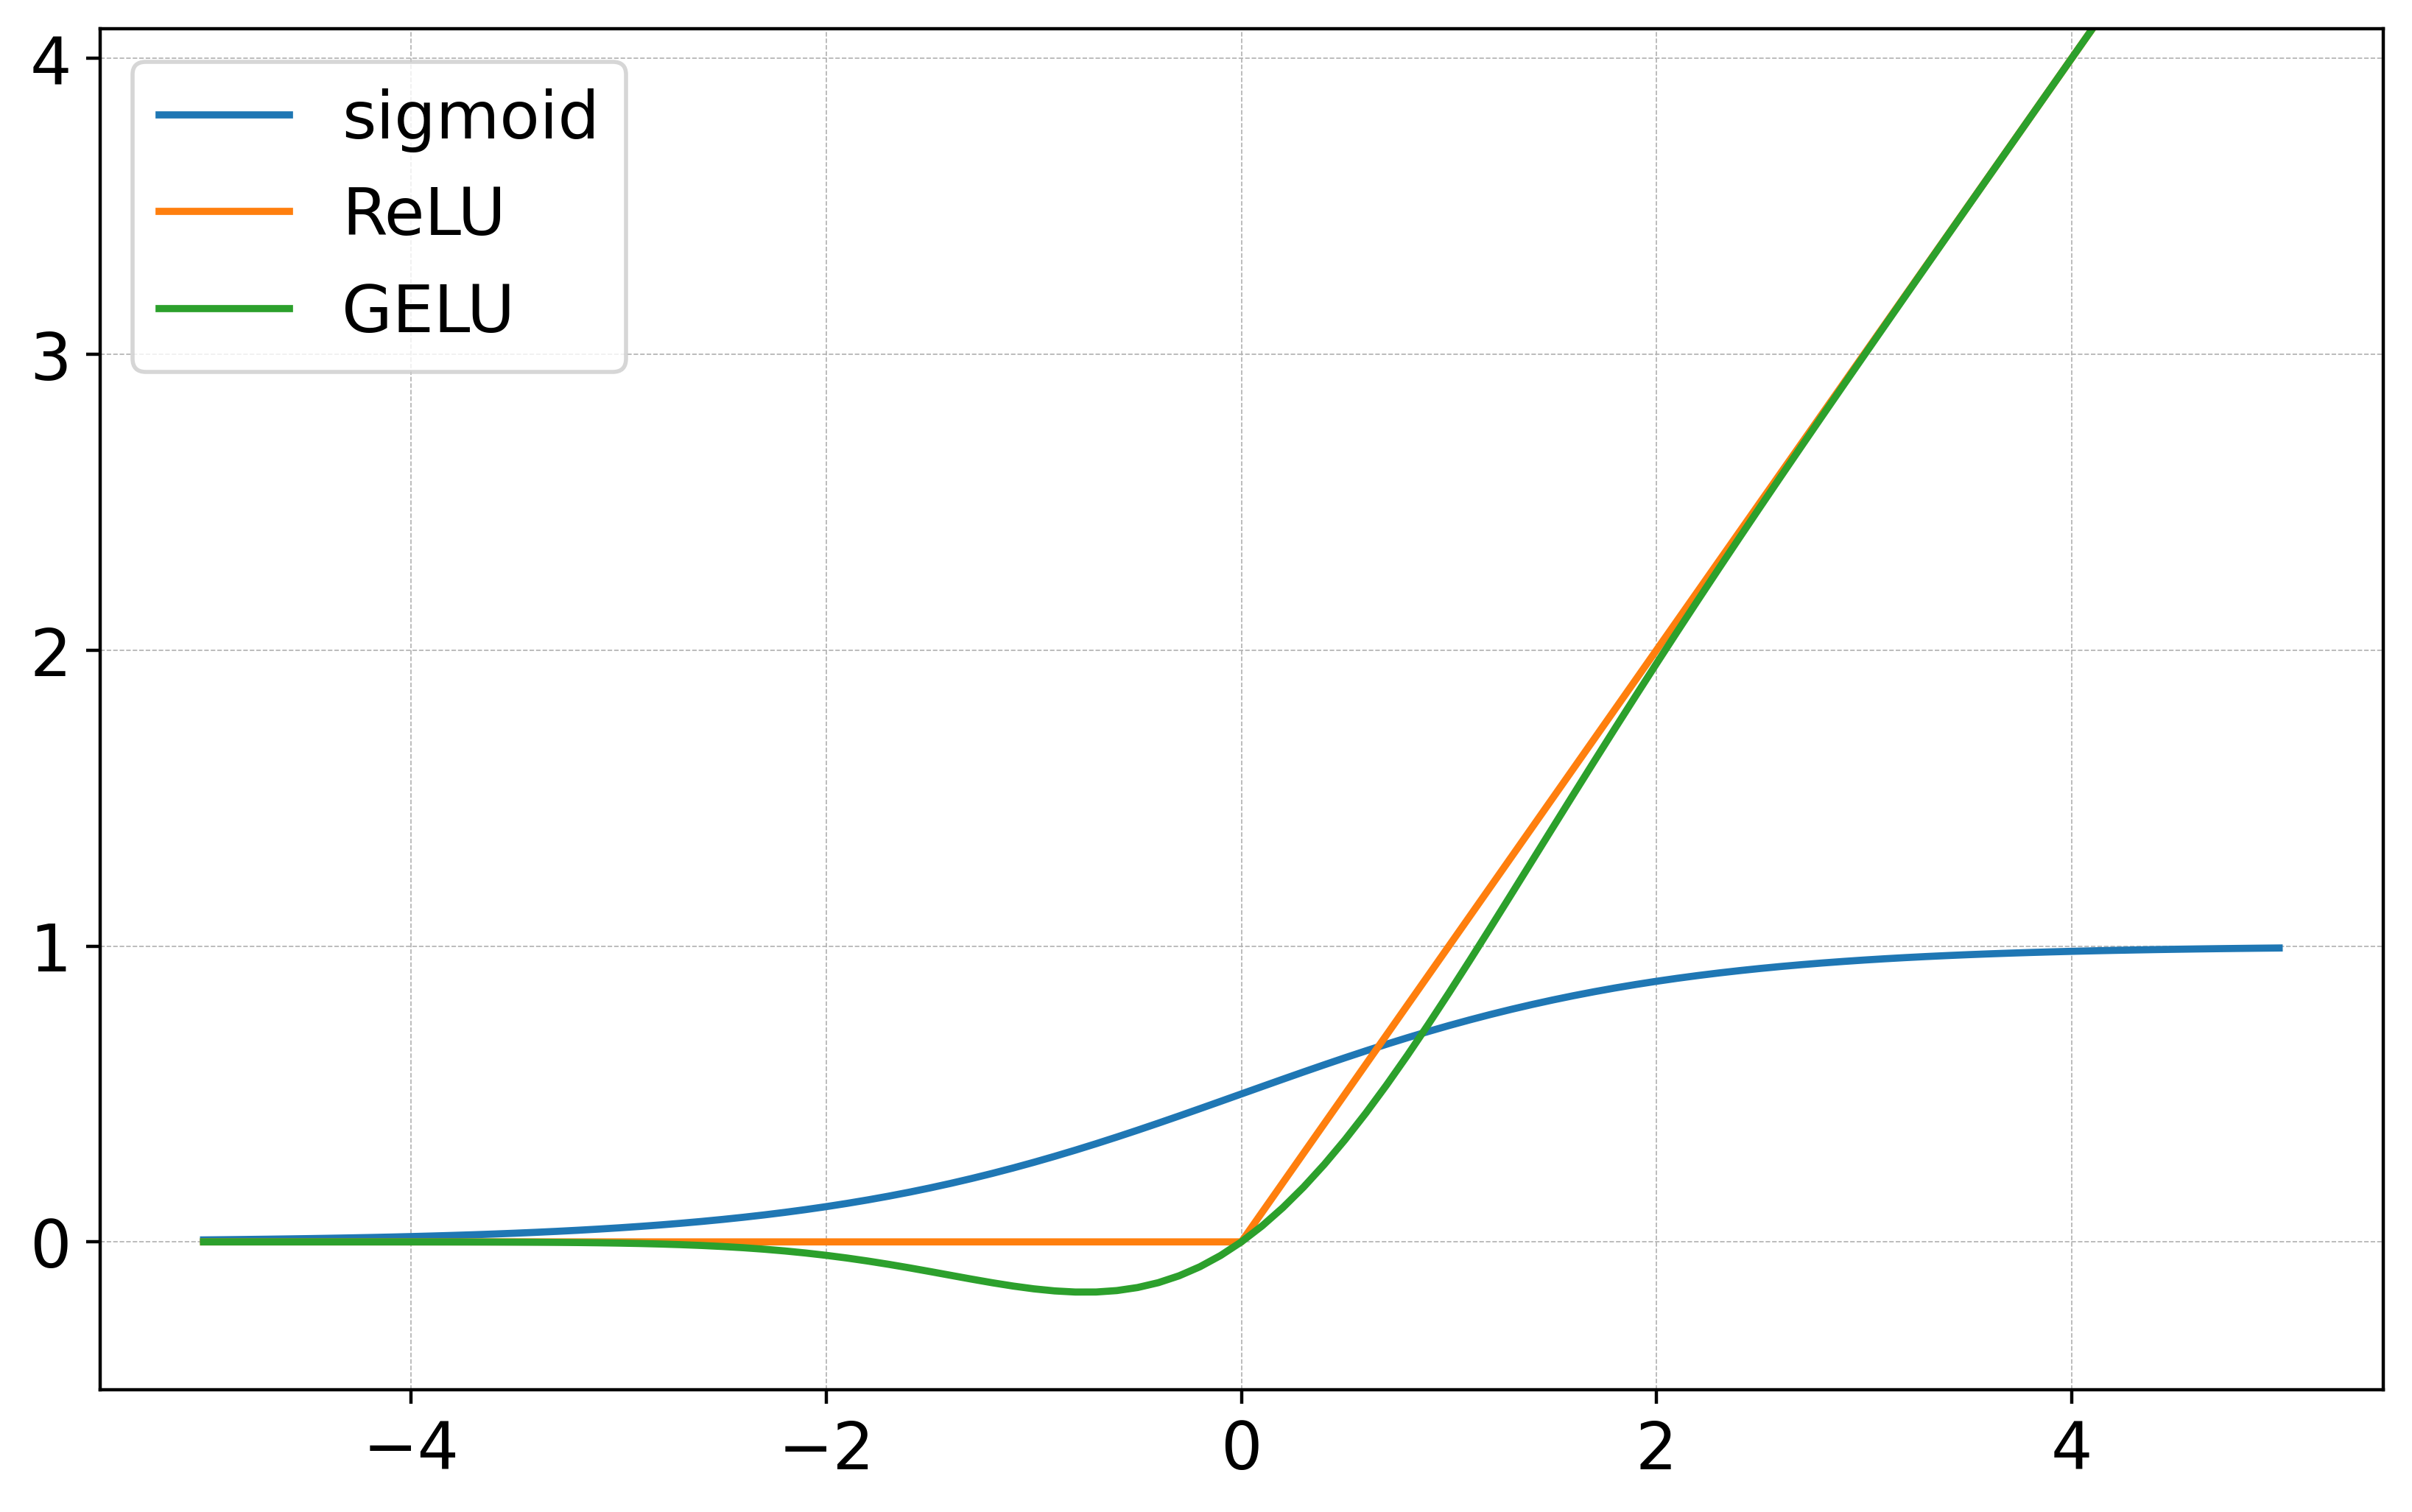
\includegraphics[width=0.7\linewidth]{figures/04_transformer/Activation_functions.png}
    \caption{Common activation functions applied to inputs in the range $x \in [-5, 5]$.}
\label{fig:Activation_functions}
\end{figure}


\subsection{Optimization}
\label{sec:03_optimization}

As seen in the case of linear regression, machine learning aims to determine the optimal parameters $\hat{\boldsymbol{\theta}}$ that describe the mapping $f(\mathbf{x}; \boldsymbol{\theta})$ given a set of input-output pairs $\{\mathbf{x}_i, \mathbf{y}_i\}$. To do so, one minimizes a loss function, a quantitative measure for the discrepancy between the model's predictions and the true target values~\cite{prince_understanding_2023}.  

One of the most widely used principles for parameter estimation is maximum likelihood estimation (MLE). In this approach, we seek the parameters ${\boldsymbol{\theta}} \in \mathcal{T}$ that maximize the likelihood of the data given the parameters. Assuming that the training samples are drawn independently from the same distribution, the likelihood function factorizes, and the MLE takes the form:
\begin{equation}
\label{eq:maximum_likelihood}
    \hat{\boldsymbol{\theta}} = \underset{\boldsymbol{\theta}}{\mathrm{argmax}} \; P\left( \mathcal{T} \mid \boldsymbol{\theta} \right) = \underset{\boldsymbol{\theta}}{\mathrm{argmax}} \prod_{i=1}^N P\left( \mathbf{y}_i \mid \mathbf{x}_i; \boldsymbol{\theta} \right)\,.
\end{equation}

In practice, working with products of probabilities is numerically unstable and analytically inconvenient. Instead, it is customary to use the negative log-likelihood (NLL) as a loss function, which transforms the product into a sum: 

\begin{equation}
\label{eq:neg_log_likelihood}
	\hat{\boldsymbol{{\theta}}} = \underset{\boldsymbol{\theta}}{\mathrm{argmin}} \; \mathrm{NLL}\left( \boldsymbol{\theta} \right) = \underset{\boldsymbol{\theta}}{\mathrm{argmin}} \; \left[ - \sum_{i=1}^N  \log P \left( \mathbf{y}_i  \mid \mathbf{x}_i; \boldsymbol{\theta} \right) \right] \,.
\end{equation}

This formulation is widely used across regression and classification tasks. In fact, the least-squares loss introduced in equation~\refeq{eq:least_squares} is a special case of equation~\refeq{eq:neg_log_likelihood}, where we assume a Gaussian likelihood with a fixed variance~\cite{murphy_probabilistic_2022, zhang_dive_2023}.


A widely used loss function in supervised classification tasks is the cross-entropy loss, which measures the dissimilarity between the empirical distribution $q(y)$ of the observed data and the predicted distribution $p(y)$ of the model. Minimizing cross-entropy is equivalent to minimizing the Kullback-Leibler divergence between the true and predicted distributions when the true distribution is fixed~\cite{prince_understanding_2023}. The cross-entropy is defined as:

\begin{equation}
\label{eq:cross_entropy}
	\mathbb{H}(q,p) = - \sum_y q(y) \log{p(y)} \,.
\end{equation}

In classification settings, the true distribution $q(y)$ is often represented as a one-hot vector, where the entry corresponding to the correct class is 1 and all others are 0. The predicted distribution $p(y)$ is typically the output of a softmax function applied to the final layer of the network. 
However, cross-entropy loss may perform poorly when the dataset is class-imbalanced, as the model is biased toward majority classes. To address this, the focal loss was introduced~\cite{lin_focal_2018}. It extends the cross-entropy by a modulating factor $(1 - p_t)^{\gamma}$, where $p_t$ is the model's predicted probability for the true class. This factor down-weights well-classified examples and focuses learning on hard, misclassified instances~\cite{lin_focal_2018}:

\begin{equation}
\label{eq:focal_loss}
	L_{\mathrm{focal}} \left( \mathbf{y}, \hat{\mathbf{p}} \right)  = - \left( 1 - \hat{p_y} \right)^{\gamma} \, \log \hat{p_y} \,.
\end{equation}

Here, $\mathbf{y}$ is the true class label (as an integer) and $\hat{\mathbf{p}}$ is a vector representing an estimated probability distribution over the classes~\cite{mavrin_artemmavrinfocal-loss_2024}. 

Another loss function commonly used in imbalanced classification problems is the Dice loss, derived from the Dice-Sørensen coefficient. It measures the overlap between predicted and true class distributions and is especially useful in segmentation tasks with extreme class imbalance, such as in medical imaging. The multi-class Dice loss is given by:

\begin{equation}
\label{eq:dice_score}
	L_{\mathrm{Dice}} = 1 - \frac{1}{N_c} \sum_{i=1}^{N_c} \frac{2 y_i \hat{p}_i + \epsilon}{y_i + \hat{p}_i + \epsilon} \,,
\end{equation}

\noindent where $\mathbf{y}, \hat{\mathbf{p}} \in \mathbb{R}^{N_c}$ represent the true and predicted class probabilities, respectively, and $\epsilon$ is a small factor to ensure this function is always well-defined. It is possible to combine different loss functions, for example, by defining a combined loss as the sum of Dice and focal loss:

\begin{equation}
\label{eq:combined_loss}
	L_{\mathrm{combined}} = L_{\mathrm{focal}} + L_{\mathrm{Dice}} \,.
\end{equation}

Taghanaki et al. showed that a weighted sum of Dice and focal loss outperforms other state-of-the-art methods in medical imaging analysis~\cite{taghanaki_combo_2019}.  



\subsubsection{Optimization algorithms}
\label{sec:03_optimization_algorithms}

Various optimization algorithms are available for minimizing the loss function, but the most fundamental is gradient descent. It works as follows: 
At each iteration $i$, the gradient of the loss with respect to the parameters is computed (equation~\refeq{eq:gradient_descent1}), and the parameters are then updated by a step of size $\alpha$ (the learning rate):

\begin{align}
\label{eq:gradient_descent1}
	\grad L & = \frac{\partial L}{\partial \theta} \,,\\
\label{eq:gradient_descent2}
	\theta_{i+1} & = \theta_i - \alpha \cdot \grad L \,.
\end{align}

When the gradient approaches zero, successive updates become negligible. In practice, most algorithms terminate if the change in parameters falls below a predefined threshold~\cite{prince_understanding_2023}.
It can be very challenging to optimize loss functions using gradient descent. If the learning rate is too small, convergence is slow, and if it's too large, the algorithm may overshoot or diverge. In high-dimensional, non-convex problems such as deep learning, plateaus, saddle points, and poor curvature are problematic~\cite{murphy_probabilistic_2022}. 

Stochastic gradient descent (SGD) reduces the computational cost and helps escape poor regions of the loss function by replacing the full gradient with an expectation over a random subset of the data:

\begin{equation}
\label{eq:stochastic_optimization}
	\mathbb{E}_{q(\mathbf{z})} \left[ L \left( \boldsymbol{\theta}, \mathbf{z} \right) \right] \,.
\end{equation}

Here, $\mathbf{z}$ denotes a mini-batch, and the expectation is taken over the empirical data distribution $q(\mathbf{z})$, which is typically approximated as uniform over the available training samples. The inherent noise introduced by this stochastic sampling not only reduces computation but also improves generalization by preventing the model from settling into sharp or narrow local minima that might overfit the training data~\cite{prince_understanding_2023}. 
Computing the gradient over a batch $\mathcal{B}$ of size $\|\mathcal{B}\|$ gives: 

\begin{equation}
\label{eq:batch_stochastic_gradient_descent}
	\grad L_{\mathcal{B}} = \frac{\partial}{\partial  \boldsymbol{\theta}} \frac{1}{\|\mathcal{B}\|} \sum_{i \in \mathcal{B}} L(\mathbf{x}_i, \boldsymbol{\theta}) \,.
\end{equation}

This notably reduces gradient variance compared to single-sample updates~\cite{zhang_dive_2023}.
Momentum incorporates a running average of past gradients. Instead of moving purely in the direction of the current gradient, the update accumulates a velocity term that reflects recent gradient history. 
This approach dampens oscillations in noisy directions and accelerates along shallow but consistent slopes. Momentum often leads to faster convergence and better traversal of narrow valleys in the loss landscape~\cite{zhang_dive_2023, murphy_probabilistic_2022}. 
Defining: 

\begin{equation}
\label{eq:momentum1}
	m_{i+1} = \beta \cdot m_i + \grad L \,.
\end{equation}

The parameters are updated via

\begin{equation}
\label{eq:momentum2}
	\theta_{i+1} = \theta_i - \alpha \cdot m_{i+1} \,,
\end{equation}

\noindent where $\beta$ is the momentum coefficient, typically $\sim 0.9$, that controls the contribution of past gradients. 

The Adaptive Moment Estimation (Adam) optimizer combines stochastic optimization and momentum~\cite{kingma_adam_2017}. For this, we define:

\begin{align}
\label{eq:ADAM1}
	\tilde m_{i+1} & = \beta_1 \cdot \tilde m_i + (1 - \beta_1) \grad L \,,\\
\label{eq:ADAM2}
	\tilde s_{i+1} & = \beta_2 \cdot \tilde s_i + (1 - \beta_2) \left(\grad L \right)^2 \,,
\end{align}

\noindent where $\tilde m_i$ is the normalized momentum and $\tilde s_i$ is the normalized second moment of the gradient. The normalization is to avoid bias at the beginning of the training, where only a few past gradients exist. It is given as $\tilde m_i = \frac{m_i}{(1 - \beta_1)}$ and analogous for $\tilde s_i$. 
The parameters are updated as follows: 

\begin{equation}
\label{eq:ADAM3}
\theta_{i+1} = \theta_i - \alpha \frac{\tilde m_i}{\sqrt{\tilde s_i} + \epsilon} \,,
\end{equation}

\noindent where $\alpha$ is the learning rate and $\epsilon$ is a small constant to avoid division by zero. The standard values are $\beta_1 = 0.9$, $\beta_2 = 0.999$, and $\epsilon = 10^{-6}$~\cite{murphy_probabilistic_2022}. Figure~\ref{fig:Optimization_plots} shows the implementation of SGD, momentum, and Adam on an ill-conditioned quadratic loss surface, $L(\boldsymbol{\theta}) = \frac{1}{2} \left( 1 \cdot {\theta^{(0)}}^2 + 0.5 \cdot {\theta^{(1)}}^2 \right)$.

\begin{figure}
    \centering
    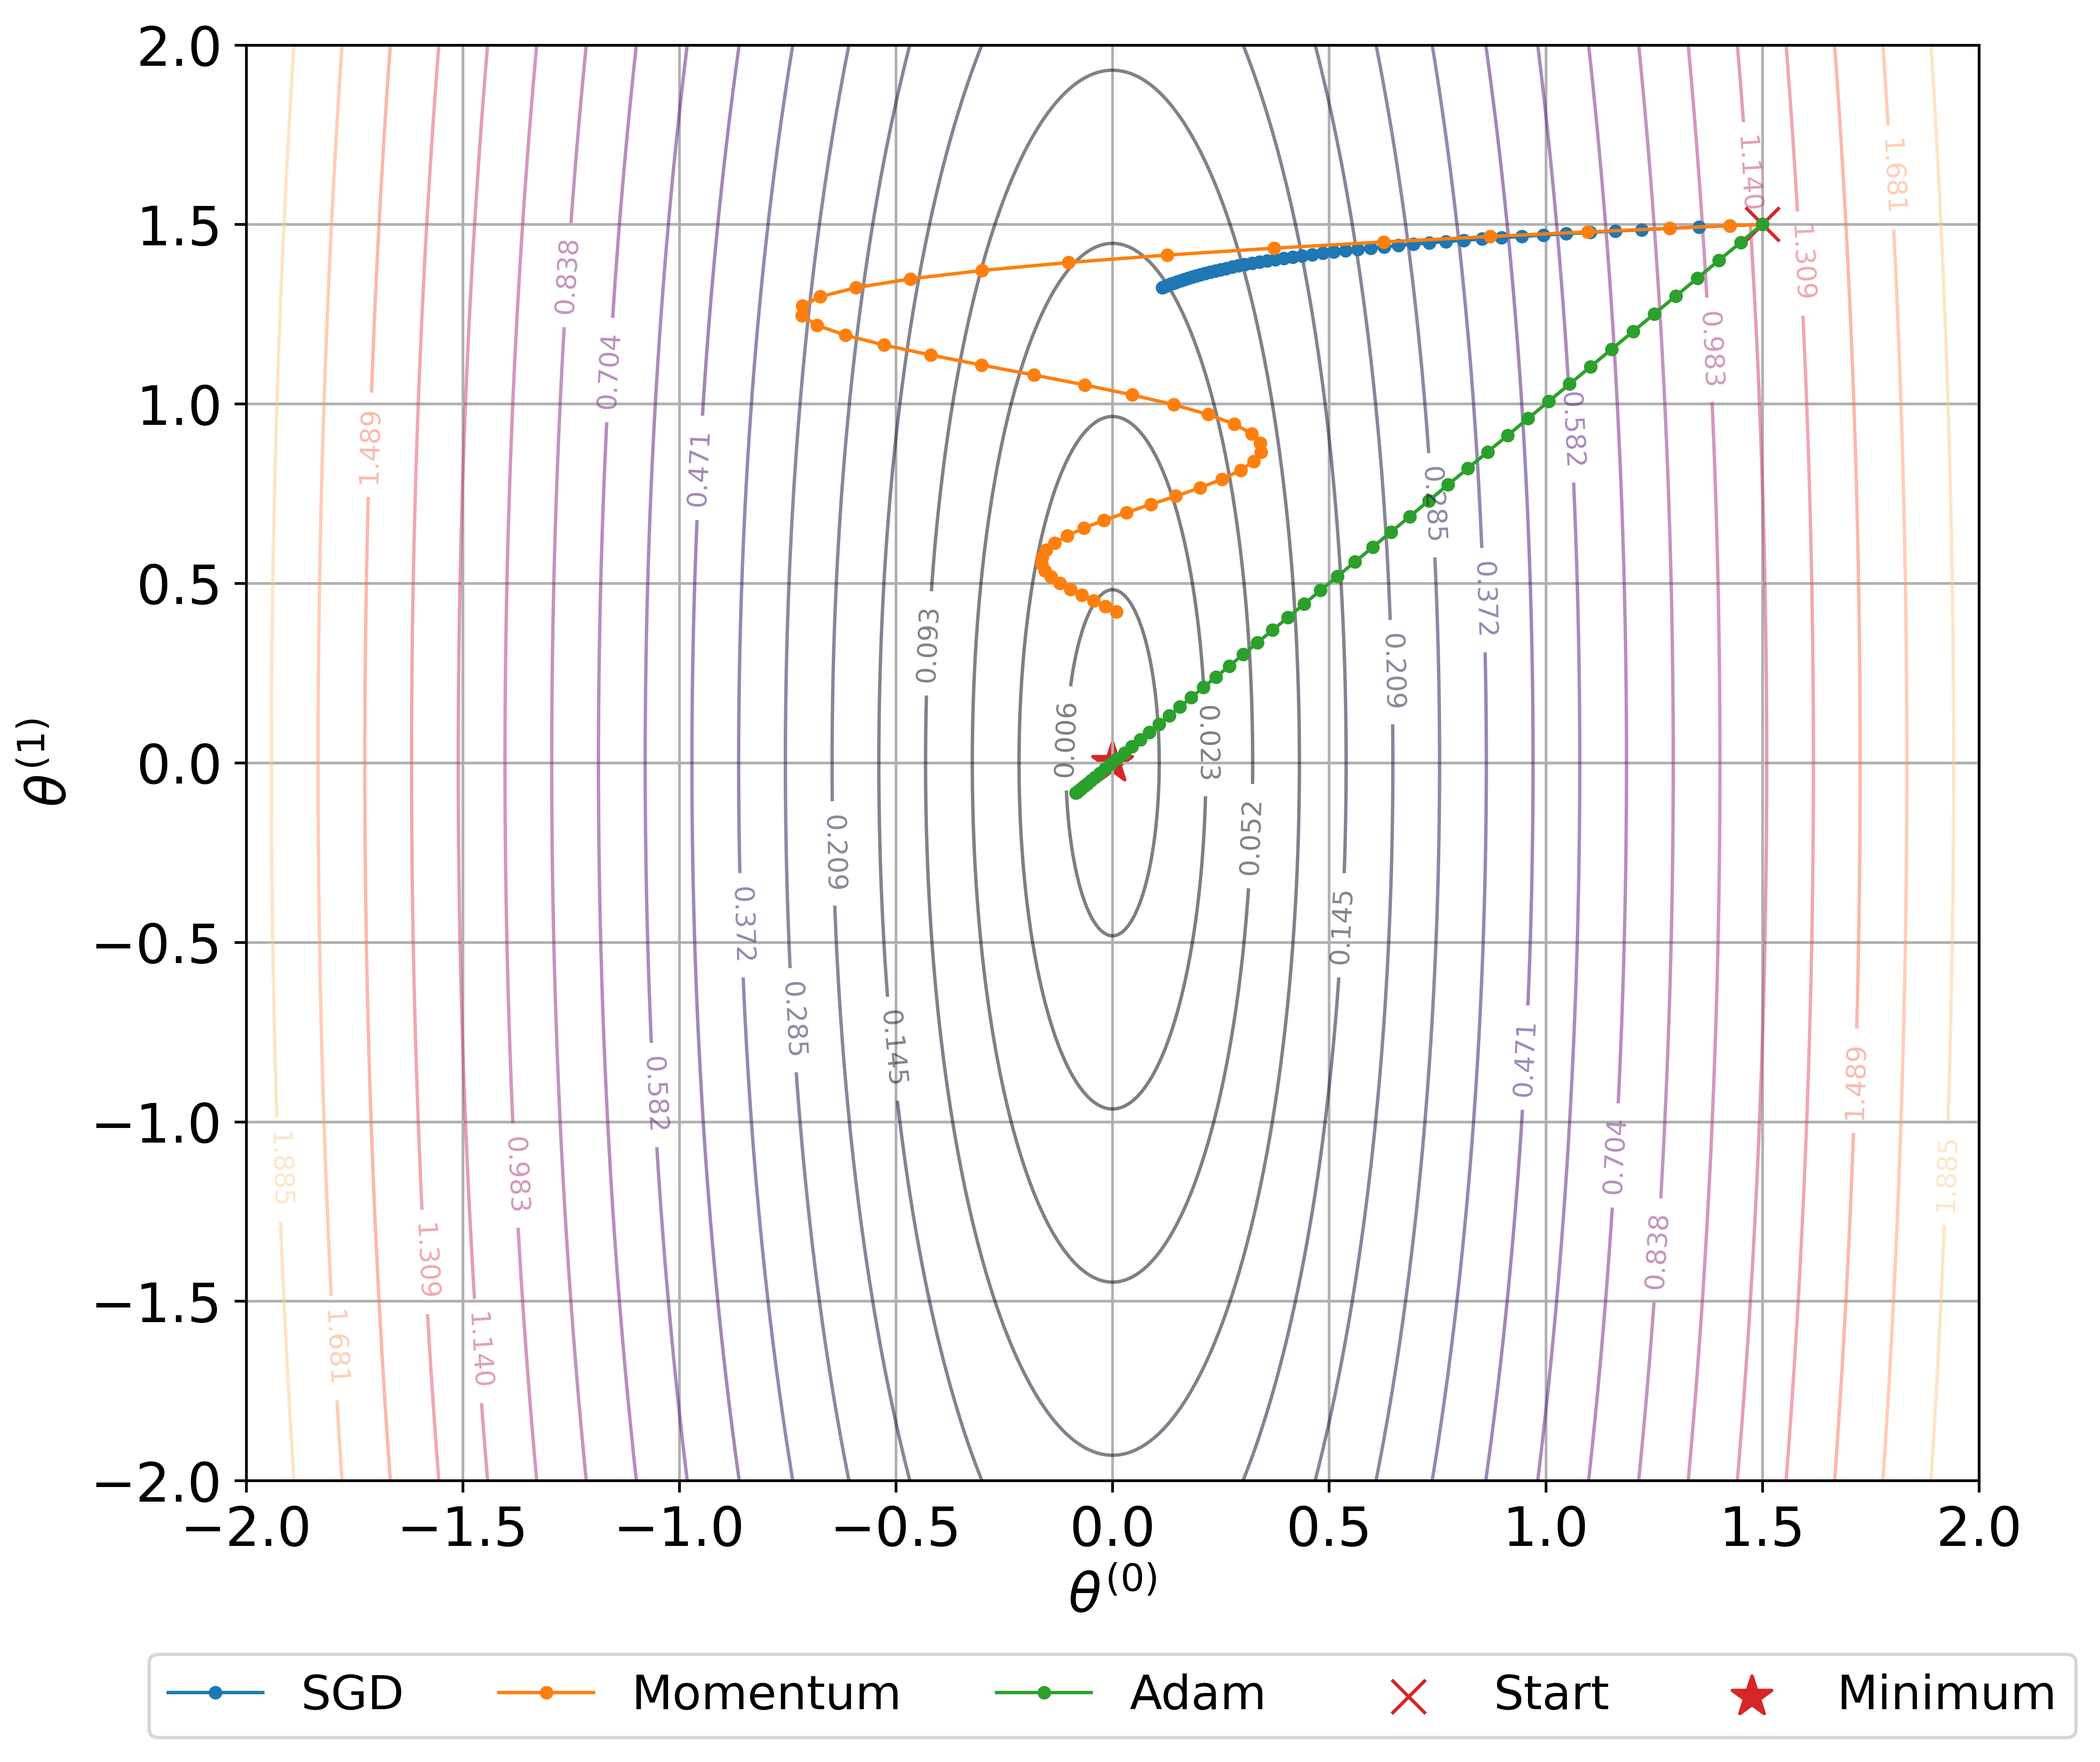
\includegraphics[width=0.85\linewidth]{figures/04_transformer/Transformer_optimization.png}
    \caption{Optimizer trajectories on an ill-conditioned quadratic loss surface, illustrating the behavior of SGD, momentum ($\beta = 0.9$) and Adam ($\beta_1 = 0.9, \; \beta_2 = 0.999$). The horizontal and vertical axes correspond to the two components of the parameter vector; colors show the loss value. SGD follows a slow path down the valley before curving toward the minimum, momentum overshoots and oscillates along the narrow direction before converging, and Adam adapts the step sizes to move almost directly toward the minimum. The number of iterations is set to 40, and the learning rate is set to $\alpha = 0.05$ for all algorithms.}
\label{fig:Optimization_plots}
\end{figure}

\subsubsection{Backpropagation}

As described in Section~\ref{sec:03_optimization_algorithms}, optimization requires calculating the gradients of the loss functions with respect to every trainable parameter in the model. In deep neural networks, the number of parameters can be in the millions. It is therefore important to compute these gradients efficiently~\cite{prince_understanding_2023}. This is the role of the well-known backpropagation algorithm. 

Let us consider the shallow neural network shown in  figure~\ref{fig:shallow_NN}, which consists of a single hidden layer. The network's operations during a forward pass can be described by the following sequence of functions:

\begin{align}
\label{eq:backprop_example_forwardpass}
	x_2 & = f_1(x; \theta_1) & \text{(linear combination)} \\ 
	x_3 & = f_2(x_2) & \text{(activation)} \\
	x_4 & = f_3(x_3; \theta_3) & \text{(linear combination)} \\
	L & = f_4(x_4, y) & \text{(loss)} 
\end{align}

\begin{figure}
    \centering
    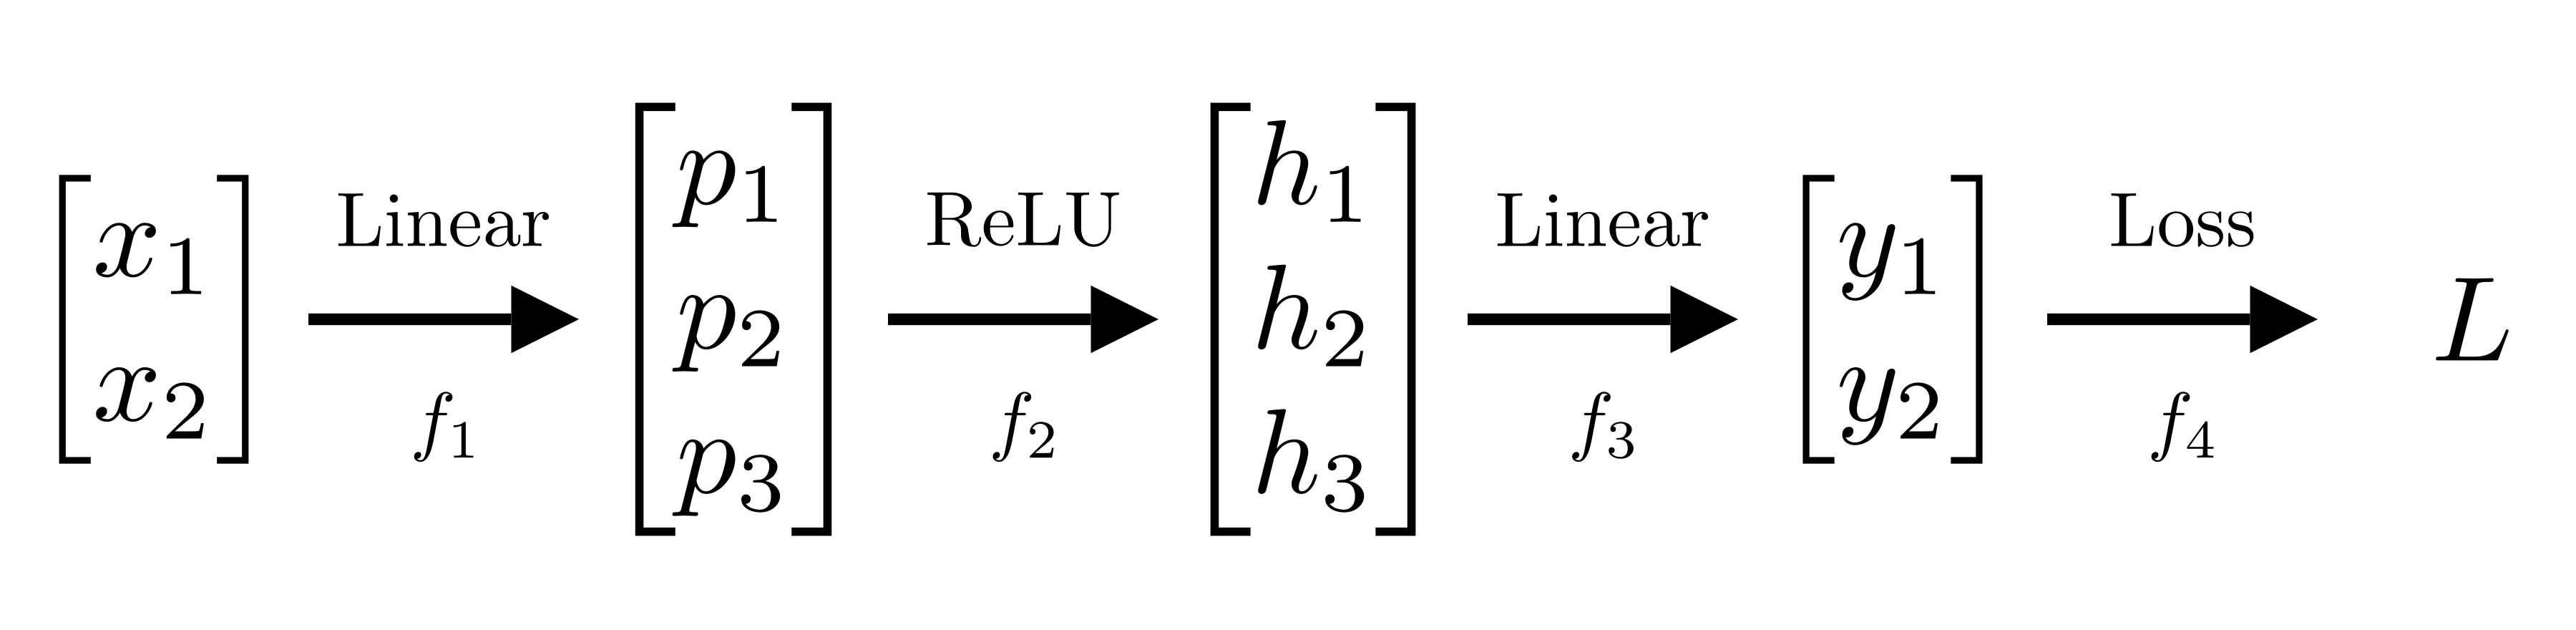
\includegraphics[width=0.85\linewidth]{figures/04_transformer/Shallow_NN_operations.png}
    \caption{Visualization of the MLP in figure~\ref{fig:shallow_NN}, where each operation is displayed separately. The hidden layer is split into pre-activation and activation. Plot created with~\cite{the_manim_community_developers_manim_2025}.}
\label{fig:shallow_NN_operation}
\end{figure}


\noindent Here, $x$ and $y$ are the input and true output, respectively. The network as a whole can be written as the composition $f = f_4 \circ f_3 \circ f_2 \circ f_1$. This is illustrated in figure~\ref{fig:shallow_NN_operation}. Note that the activation function $f_2$ has no trainable parameters, as it only introduces a non-linearity. 

Already small changes to parameters can be amplified as they propagate through the network. To compute how a change in a parameter, such as $\theta_3$ affects the loss, we need to know how intermediate quantities like $x_4$ respond. 
For a parameter further away from the output, such as $\theta_1$, the influence must be computed through a chain of dependencies: From $x_2$ to $x_3$, from $x_3$ to $x_4$, and finally from $x_4$ to the loss. 
The backpropagation algorithm exploits this structure: Rather than recomputing gradients from scratch at every layer, it reuses intermediate results. This leads to significant computational savings. The backward pass proceeds from the output layer back toward the input:

\begin{align}
\label{eq:backprop_example_backwardpass}
	\frac{\partial L}{\partial \theta_3} & = \frac{\partial L}{\partial x_4} \frac{\partial x_4}{\partial \theta_3} \,,\\
	\frac{\partial L}{\partial \theta_1} & = \frac{\partial L}{\partial x_4} \frac{\partial x_4}{\partial x_3} \frac{\partial x_3}{\partial x_2} \frac{\partial x_2}{\partial \theta_1} \,.
\end{align}

Each $\frac{\partial L}{\partial \theta_k}$ is a row vector that can be computed recursively by propagating the upstream gradient through the network. Specifically, it is obtained by multiplying the gradient from the previous layer of the Jacobian $\frac{\partial x_k}{\partial x_{k-1}}$, which captures how changes in the input layer $k -1$ affect the output of layer $k$. This recursive structure enables efficient computations of gradients.
The Jacobian matrix itself is defined as:


\begin{equation}
\label{eq:backprop_jacobian}
	\mathbf{J_f} =  
\begin{pmatrix} 
\frac{\partial f_1}{\partial x_1} & \cdots & \frac{\partial f_1}{\partial x_n} \\
\vdots & \ddots & \vdots \\
\frac{\partial f_m}{\partial x_1} & \cdots &  \frac{\partial f_m}{\partial x_n} \\
\end{pmatrix} 
	= \begin{pmatrix} \grad f_1 (\mathbf{x})^{\intercal} \\ \vdots \\ \grad f_m(\mathbf{x})^{\intercal} \end{pmatrix}
	= \begin{pmatrix} \frac{\partial \mathbf{f}}{\partial x_1 } \ldots \frac{\partial \mathbf{f}}{\partial x_n}\end{pmatrix} \in \mathbb{R}^{m \times n} \,.
\end{equation}

Depending on the dimensions of the input $n$ and output $m$, the Jacobian is calculated differently. If $n < m$, it is more efficient to calculate each row $\frac{\partial \mathbf{f}}{\partial x_j}$. 
However, in practice, scalar outputs are common ($m = 1$), making it more efficient to compute the Jacobian columns $\grad f_i(x)^{\intercal}$. 

The backward algorithm then proceeds recursively, starting from $u_{K+1}^{\intercal} = 1$ and iterating $k$ from $K$ to 1:

\begin{align}
\label{eq:backprop_backwardpass}
	g_k & = u_{k+1}^{\intercal} \frac{\partial \mathbf{f}_k(x_k, \theta_k)}{\partial \theta_k} \,,\\
	u_k^{\intercal} & = u_{k+1}^{\intercal} \frac{\partial \mathbf{f}_k(x_k, \theta_k)}{\partial x_k} \,. 
\end{align}

This algorithm is computationally very efficient, as the most expensive operations are matrix multiplications, which can be parallelized and executed rapidly on modern hardware. 


\subsubsection{Traning stability}
Despite the efficiency of the backpropagation algorithm, training large neural networks remains challenging. During backpropagation, gradients are computed using the chain rule and propagated recursively through each layer.
However, if these derivatives are small, their repeated multiplication can lead to vanishing gradients, where gradients become too small to update parameters effectively. Similarly, very large derivatives can result in exploding gradients, where parameters become unstable. 
The latter can be controlled using gradient clipping, where gradients exceeding a certain threshold $c$ are scaled down~\cite{murphy_probabilistic_2022}:

\begin{equation}
\label{eq:gradient_clipping}
    \mathbf{g}' = \min(1, \frac{c}{\norm{\mathbf{g}}}) \, \mathbf{g} \,,
\end{equation}

\noindent where $\mathbf{g}'$ is the scaled gradient that goes in the same direction as the gradient $\mathbf{g}$.


The vanishing gradient can be mitigated by using a loss function whose gradient is not too small, which is the case for ReLU and GELU.  
An effective approach is the use of residual connections, illustrated in figure~\ref{fig:ResidualMLP}. In a residual network, each perceptron computes:

\begin{equation}
\label{eq:residual_layer}
	\mathcal{F'}(x) = \mathcal{F}(x) + x\,,
\end{equation}

\noindent where $\mathcal{F}(x)$ is the standard non-linear transformation (e.g., a layer or network), as defined earlier in equation~\refeq{eq:NN_hiddenlayer}~\cite{he_deep_2015}. While this does not increase the number of trainable parameters, it improves trainability~\cite{murphy_probabilistic_2022}. 
To see this, consider the gradient in the residual case:

\begin{figure}[t]
    \centering
    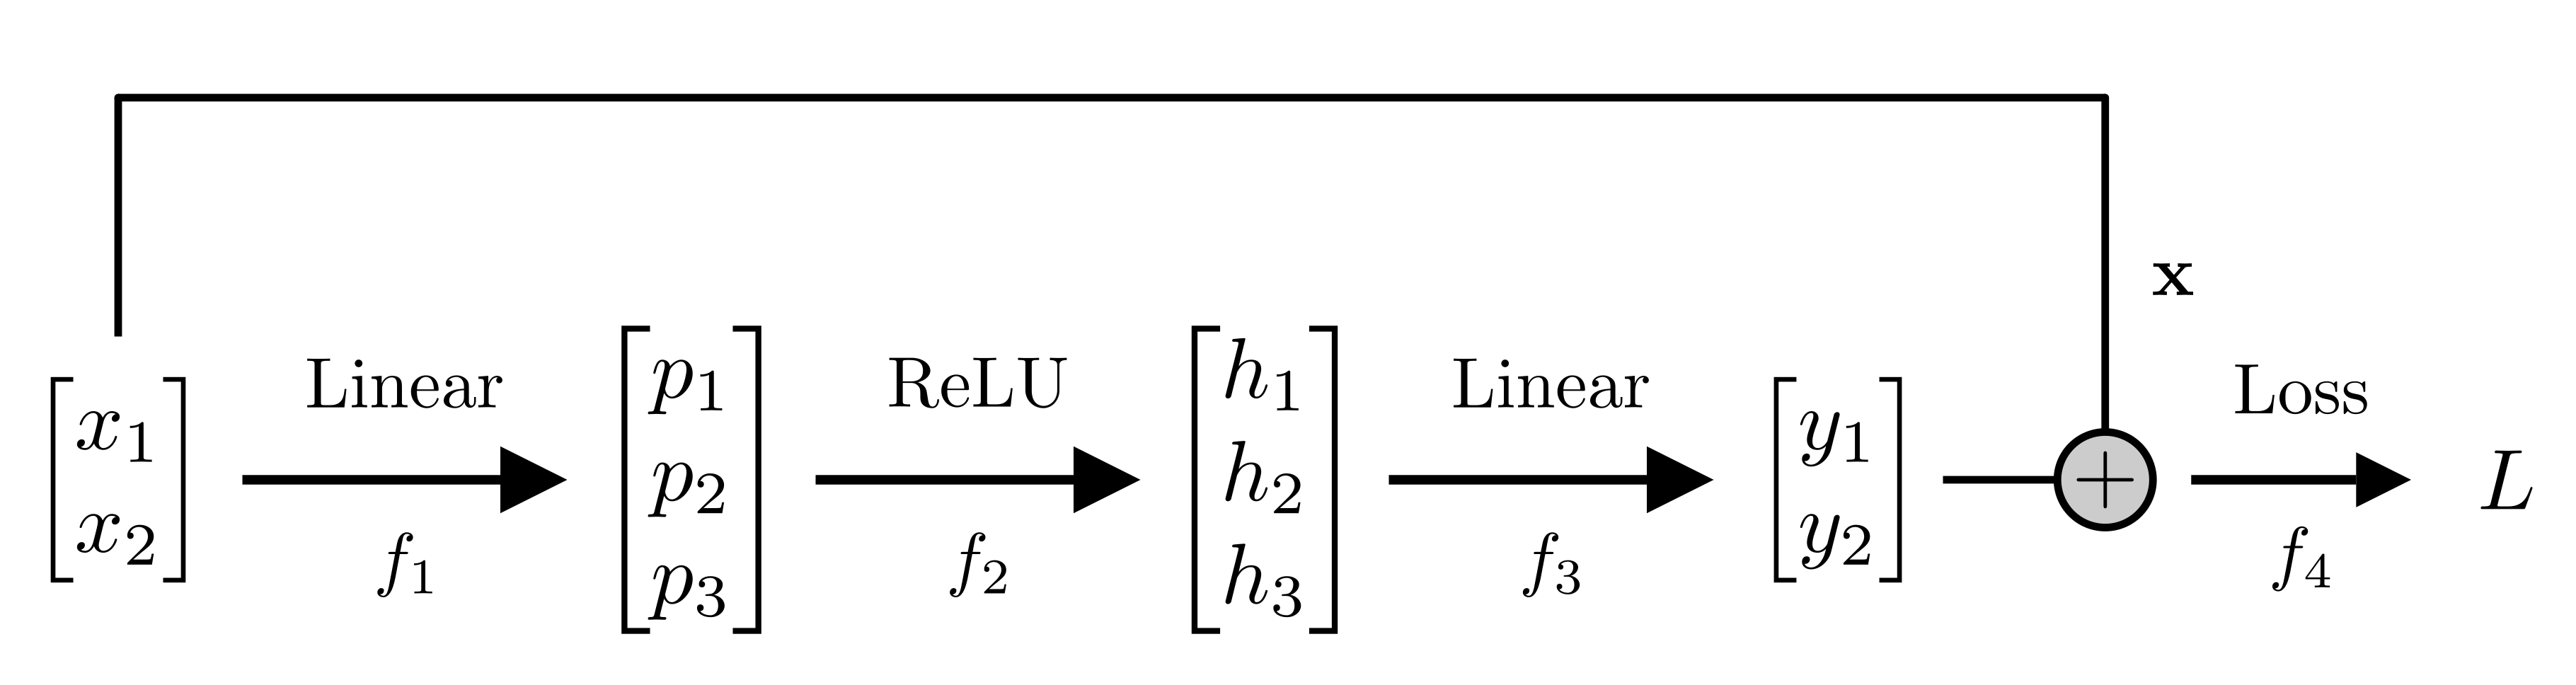
\includegraphics[width=0.95\linewidth]{figures/04_transformer/ResidualMLP.png}
    \caption{Multilayer perceptron of figure~\ref{fig:shallow_NN_operation}, but including a residual connection, which is indicated by the line adding $\mathbf{x}$ to the output $\mathbf{y}$. Plotted with~\cite{the_manim_community_developers_manim_2025}.}
\label{fig:ResidualMLP}
\end{figure}


\begin{equation}
\label{eq:backprop_resnet}
	\frac{\partial L}{\partial \theta_3} = \frac{\partial L}{\partial x_4} \frac{\partial x_4}{\partial x_3} \frac{\partial x_3}{\partial \theta_2} = \frac{\partial L}{\partial x_4} \left( \frac{\partial f_3}{\partial x_3} + \mathbb{1} \right) \frac{\partial x_3}{\partial \theta_2} \,.
\end{equation}

The identity term $\mathbb{1}$ arises because $x_3$ is directly added to $f_3$. Hence even if $\frac{\partial f}{\partial x_3}$ is very small, the gradient will not vanish~\cite{murphy_probabilistic_2022}.

Another key technique to improve numerical stability is normalization. Two commonly used methods are batch normalization and layer normalization. 

Batch normalization standardizes the pre-activations to zero mean and unit variance. Recall that the equation for a hidden unit in a fully connected NN was $h_d = F \left[ \mathbf{b}_\theta + \mathbf{W}_{\theta} \cdot \mathbf{x} \right]$. 
We can add a batch normalization as follows: 

\begin{equation}
\label{eq:NN_hidden_unit_BN}
	h_d = F \left[ \mathrm{BN}(\mathbf{b}_\theta + \mathbf{W}_{\theta} \cdot \mathbf{x}) \right] \,.
\end{equation}

For a given batch $\mathcal{B}$ the batch normalization is defined as:

\begin{equation}
\label{eq:BN_def}
	\mathrm{BN}(\mathbf{x}) = \gamma \circ \frac{\mathbf{x} - \mathbf{\mu_{\mathcal{B}}}}{\mathbf{\sigma_{\mathcal{B}}}} + \beta \,,
\end{equation}

\noindent Here $\mu_{\mathcal{B}}$ and $\sigma_{\mathcal{B}}$ indicate the mean and the standard deviation of the batch, calculated as in equations~\refeq{eq:BN_mean} and~\refeq{eq:BN_std} where $\epsilon$ is again a small parameter (we used $\epsilon = 10^{-5}$) to avoid division by zero.
This introduces two new parameters $\gamma$ and $\beta$ that are learned during training~\cite{zhang_dive_2023, murphy_probabilistic_2022}.

\begin{align}
\label{eq:BN_mean}
	\mu_{\mathcal{B}} & = \frac{1}{\|\mathcal{B}\|} \sum_{x \in \mathcal{B}} \mathbf{x} \,,\\
\label{eq:BN_std}
	\sigma_{\mathcal{B}} & = \sqrt{\frac{1}{\|\mathcal{B}\|} \sum_{x \in \mathcal{B}} \left( x - \mu_{\mathcal{B}} \right)^2 + \epsilon} \;.
\end{align}

Batch normalization works well for large enough batch sizes. Layer normalization is defined similarly. However, the normalization is applied over all the hidden units in a single layer of a single vector $\mathbf{x}$, making it independent of batch size. It works well for recurrent and Transformer-based models because it avoids dependence on batch-level statistics, which may be unstable or poorly defined when working with variable-length sequences or in small batch sizes, common in NL and sequence modelling. The mean and variance are computed as:

\begin{align}
\label{eq:LN_mean}
	\mu_{\mathcal{L}} &  = \frac{1}{H} \sum_{i=1}^{H} x_i \,, \\
\label{eq:LN_std}
	\sigma_{\mathcal{L}}^2 & = \frac{1}{H} \sum_{i=1}^H \left( x_i - \mu_{\mathcal{L}} \right)^2 \,,
\end{align}

\noindent where $H$ is the number of hidden units and $x_i$ refers to the activation of the i-th hidden unit in the current layer. Both $\mu_{\mathcal{L}}$ and $\sigma_{\mathcal{L}}^2$ are scalars. As with batch normalization, learnable scale and shift parameters $\gamma$ and $\beta$ are applied~\cite{zhang_dive_2023, ba_layer_2016}.  



\subsection{The Transformer network}

Although MLPs are very powerful in approximating any function, they are limited in their ability to capture relationships across structured or sequential input. In particular, when the input consists of temporally ordered data such as waveforms, MLPs struggle to model long-range dependencies. This limitation motivates the use of architectures specifically designed for such data structures, such as the Transformer network, which was introduced by Vaswani et al. in 2017~\cite{vaswani_attention_2023}. Unlike previous neural network models for sequential data, the Transformer relies exclusively on attention mechanisms. However, later variants reintroduce these components for efficiency or domain-specific modelling. 
Initially developed for natural language processing, Transformer models have since been successfully adapted to a wide variety of domains. Prominent examples include AlphaFold for protein folding~\cite{madani_large_2023}, DALL-E for image generation~\cite{parmar_image_2018}, and large language models such as ChatGPT~\cite{openai_gpt-4_2024}. 

Transformers typically follow an encoder-decoder structure. However, depending on the specific task, encoder-only or decoder-only architectures are often sufficient. For instance, ChatGPT uses a decoder-only model, whereas the Transformer used in this work relies only on an encoder. 


\begin{figure}
    \centering
    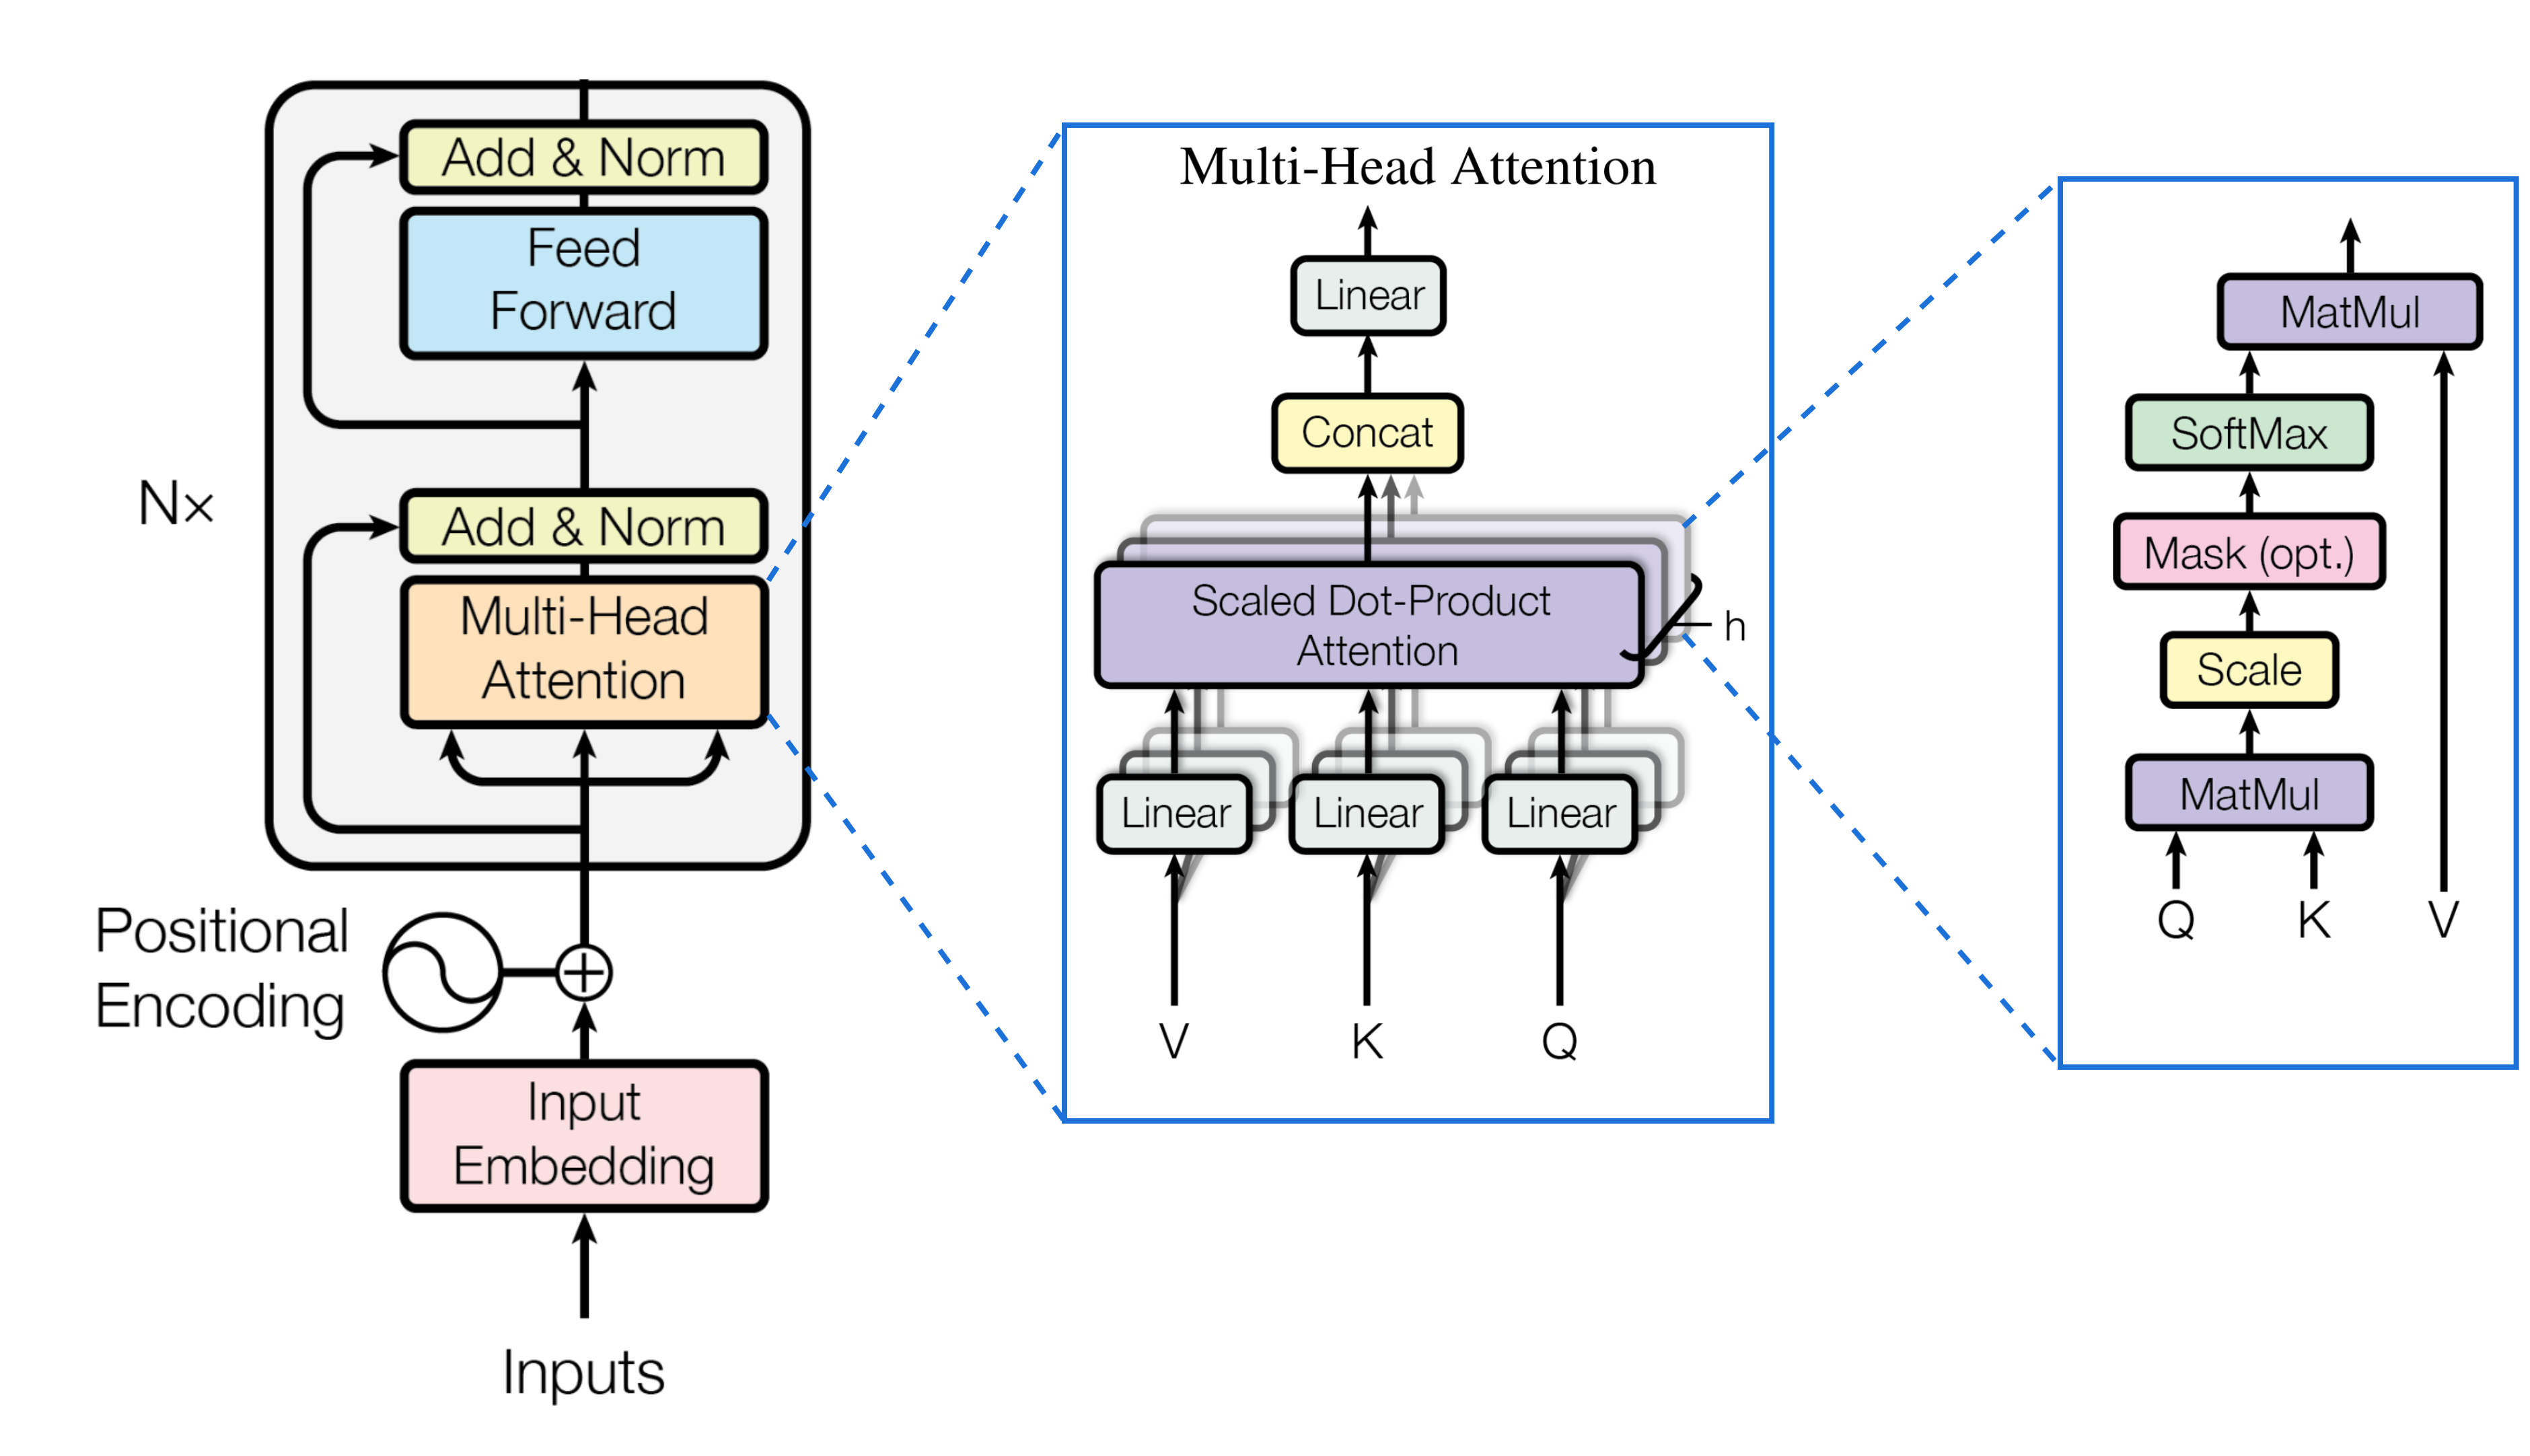
\includegraphics[width=0.95\linewidth]{figures/04_transformer/Transformer_overview.png}
    \caption{Overview of the Transformer encoder. In the first step, the inputs are embedded and positional encodings are added. Each of the $N_x$ encoder blocks contains a multi-head attention mechanism and a feedforward network. Both components are followed by layer normalization and are wrapped in residual connections, indicated by the arrows pointing to the Add \& Norm blocks. The middle panel shows the multi-head attention mechanism in more detail. Queries, keys, and values are computed by linearly transforming the inputs with their respective weight matrices. Scaled dot-product attention is then applied to these projections, and the outputs from all attention heads are concatenated and linearly transformed. The right panel illustrates the computational steps of scaled dot-product attention. This figure is adapted from~\cite{vaswani_attention_2023}.}
\label{fig:transformer_encoder}
\end{figure}

Figure~\ref{fig:transformer_encoder} illustrates an encoder-only Transformer model. The input sequence is first divided into tokens, where a token can represent a word fragment, a segment of a protein sequence, or a portion of a waveform. Each token is mapped to an embedding vector. Before entering the encoder blocks, positional encoding is added to these embeddings. 

The encoder consists of a series of identical encoder blocks, each composed of a multi-head attention mechanism followed by a feedforward network. The feedforward component closely resembles the multilayer perceptron described in section~\ref{sec:03_mlp}. 
Both components are wrapped in residual connections and followed by layer normalization, which together is denoted as Add \& Norm. Decoder blocks use similar structures but are more complex and not discussed here~\cite{murphy_probabilistic_2022, prince_understanding_2023, vaswani_attention_2023}.


\subsubsection{Input representation}
\label{sec:03_input_representation}

The input sequence is split into $n_t$ sub-sequences called tokens. In natural language processing applications, each token is then typically mapped to a learned embedding vector $\mathbf{x} \in \mathbb{R}^{d_{\mathrm{emb}}}$ representing semantic or contextual features in a continuous vector space. All token embeddings are stored in a matrix $\mathbf{T} \in \mathbb{R}^{d_{\mathrm{emb}} \times n_t}$, where each column corresponds to a token embedding~\cite{zhang_dive_2023, prince_understanding_2023}.
In contrast, our approach operates on fixed-length time-series data. Each waveform is divided into equally sized segments of 10 consecutive ADC samples, resulting in 140 uniformly spaced tokens per waveform. Each token is then projected into a 128-dimensional embedding vector via a learnable linear transformation. Using lower-dimensional embeddings can reduce training complexity but may result in underfitting. Conversely, higher-dimensional embeddings increase computational cost and risk of overfitting. 

Because attention mechanisms are inherently permutation-invariant, they lack information about the order of input tokens. Positional encoding addresses this by injecting sequence order into the model. 

The  positional encoding is implemented as a matrix $\mathbf{PE} \in \mathbb{R}^{n_t \times d_{\mathrm{emb}}}$, where $n_t$ is the number of tokens and $d_{\mathrm{emb}}$ the embedding dimension. Each row corresponds to a token and each column to a position in the embedding space~\cite{zhang_dive_2023}.
Vaswani et al. proposed a sinusoid positional embedding, where the elements are computed as:

\begin{align}
\label{eq:positional_encoding_even}
	\mathrm{PE}_{ \,i, \, 2j} & = \sin \left( \frac{i}{C^{2j/d}} \right) \,,\\
\label{eq:positional_encoding_odd}
	\mathrm{PE}_{\, i, \, 2j+1} & = \cos \left( \frac{i}{C^{2j/d}} \right)	\,,
\end{align}

\noindent where $i$ is the token index, $j$ is the embedding dimension, and $C$ is a scaling constant. We use the common choice of $C = 10^4$, which is long enough to provide a wide range of frequency scales, allowing the model to capture both short- and long-range dependencies in the sequence. Since even indices are computed with sine and odd ones with cosine, $j$ runs up to $(d/2 -1)$~\cite{vaswani_attention_2023, murphy_probabilistic_2022}. The resulting positional encoding is shown in  figure~\ref{fig:positional_encoding}.


\begin{figure}[t]
    \centering
    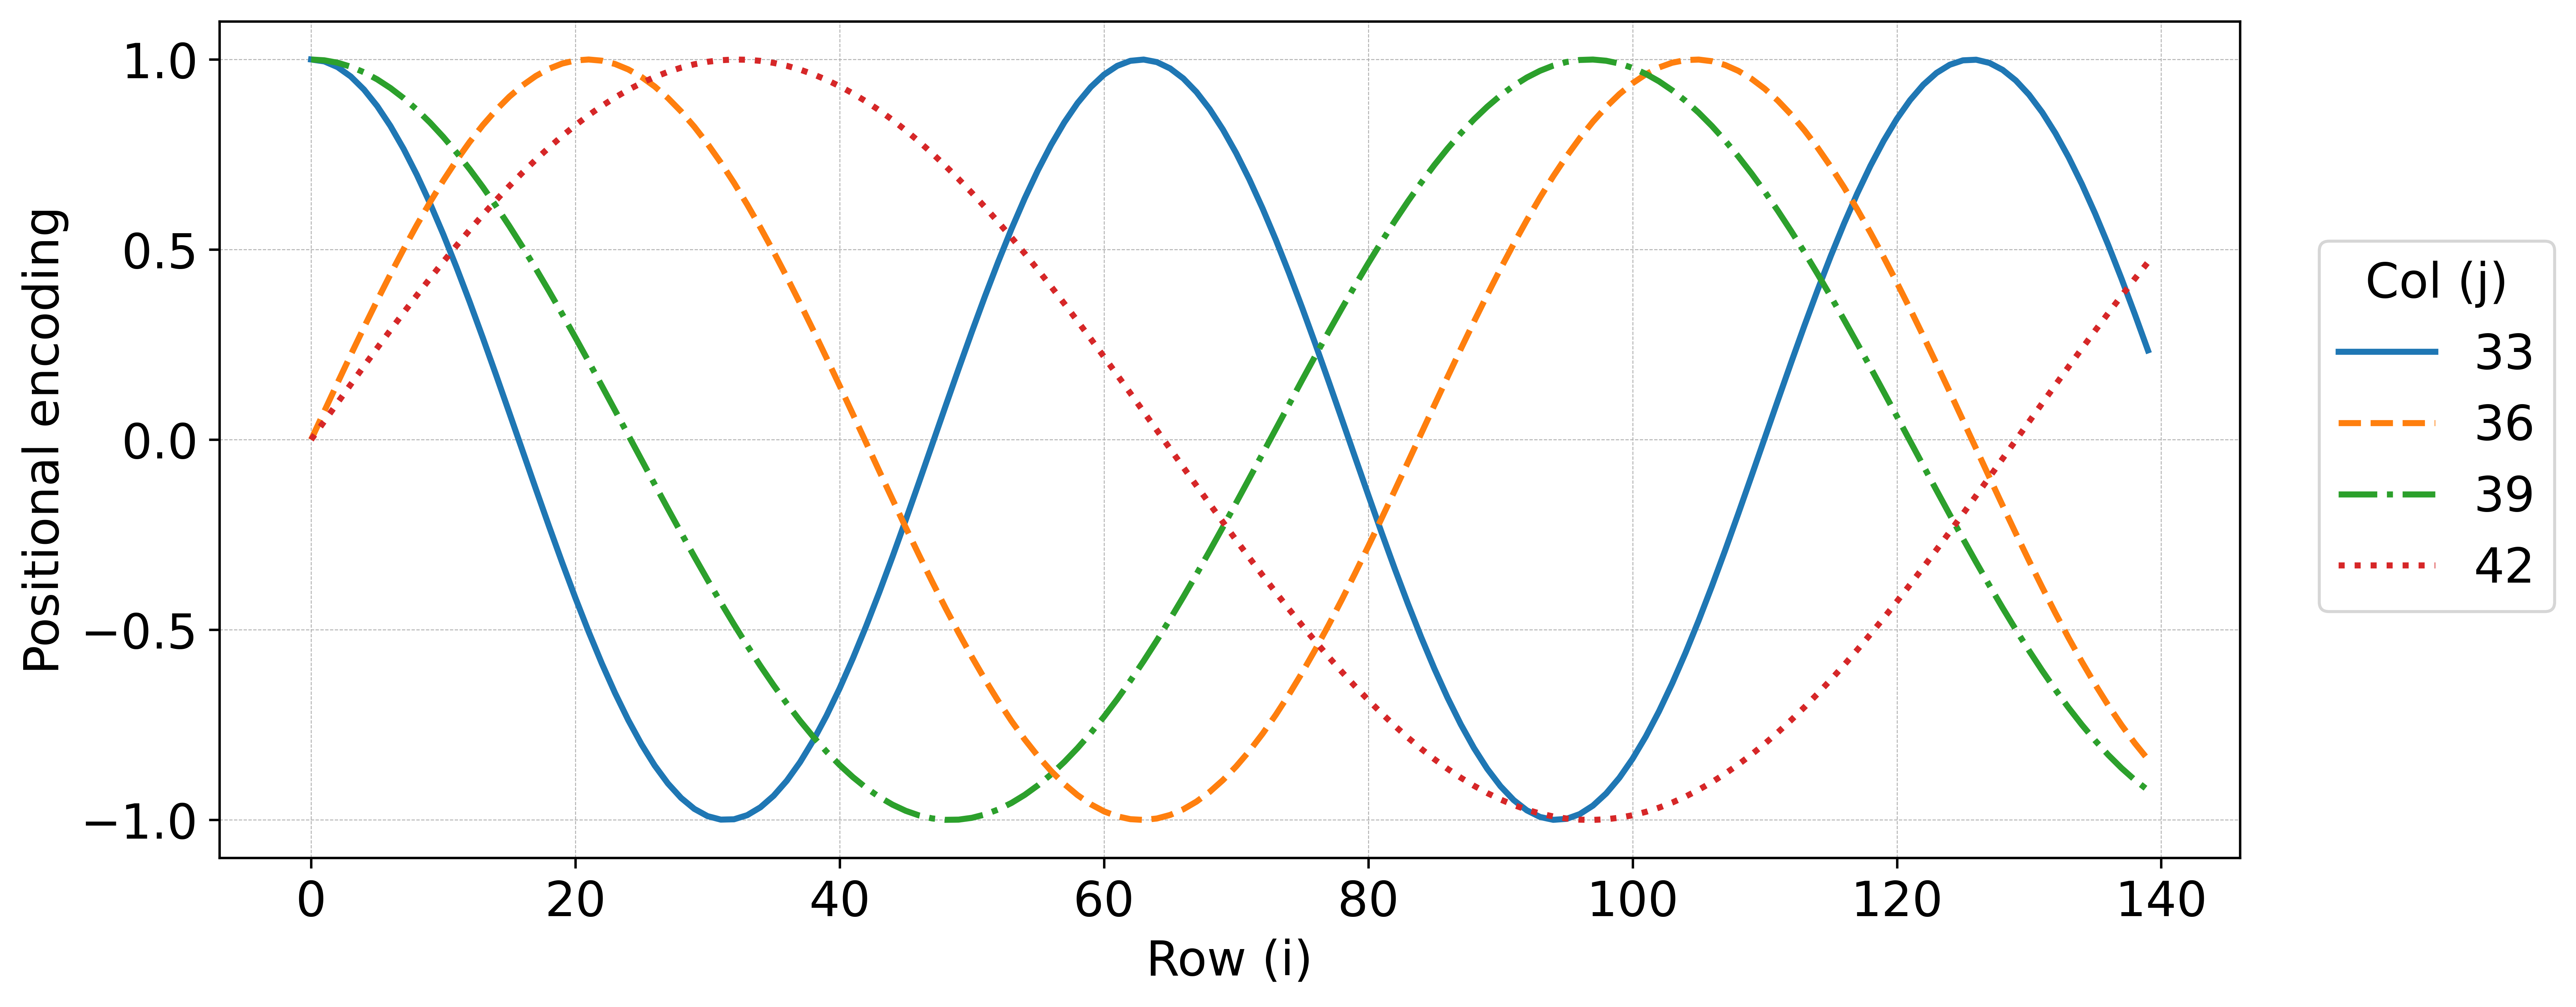
\includegraphics[width=0.95\linewidth]{figures/04_transformer/Positional_encoding.png}
    \caption{Sinusoidal positional encoding used in this work. Note that higher dimensions (columns) encode lower-frequency information. Even columns start at 0, and odd columns start at 1.} 
\label{fig:positional_encoding}
\end{figure}

Although seemingly complex, this encoding offers two major advantages. First, it allows for arbitrary sequence lengths up to $C$ without retraining. Second, the encoding for one position can be linearly computed from another. This linearity allows the model to reason about relative positions and extrapolate to unseen sequence lengths, which supports better generalization in tasks involving variable-length inputs~\cite{murphy_probabilistic_2022, vaswani_attention_2023}. For example, in a low-dimensional case with $d=2$ and $C=1$, the positional encoding $k$ steps away from position $p$ is:

\begin{align}
	\begin{pmatrix} \mathrm{PE}_{p + k, \, 0} \\ \mathrm{PE}_{p+k, \, 1} \end{pmatrix} & = 
	\begin{pmatrix} \sin \left( p + k \right) \\ \cos \left( p + k \right) \end{pmatrix} = 
	\begin{pmatrix}  \sin p \cos k + \cos p \sin k \\ \cos p \cos k - \sin p \sin k  \end{pmatrix} \\
	& = \begin{pmatrix} \cos k & \sin k \\ -\sin k & \cos k \end{pmatrix} \begin{pmatrix} \sin p \\ \cos p \end{pmatrix} \,.
\end{align}

\noindent Once computed, positional encodings are added to the embeddings $\mathbf{x}$: 

\begin{equation}
\label{eq:pos_enc_add}
    \mathbf{\tilde x} = \mathbf{x} + \mathbf{PE} \,.
\end{equation}


\subsubsection{Attention mechanism}
\label{sec:03_attention_mechanism}

The multilayer perceptron described in section~\ref{sec:03_mlp} applies a linear transformation to the input vector $\mathbf{x}$, followed by an activation function $F$. Each layer has its own set of learnable parameters.

The attention mechanism takes a different approach. Conceptually, it operates like a database: Given a set of $N$ keys $\mathbf{k}_i$ and values $\mathbf{v}_i$, a query vector $\mathbf{q}$ is used to retrieve information. 
This design allows the model to process variable-length input sequences and dynamically adapt the output based on contextual relevance. When every token attends to every other token, this mechanism allows each token to incorporate information from all other tokens, regardless of distance. This property makes attention particularly powerful for capturing long-range dependencies in sequential data. 
The general form of attention is:

\begin{equation}
\label{eq:attention}
	\mathrm{Attn}[\mathbf{q}] = \sum_{i=1}^{N} \alpha \left[ \mathbf{q}, \mathbf{k}_i \right] \, \mathbf{v}_i
\end{equation}

Here, attention is a weighted sum over the values, where each scalar weight $\alpha \left[ \mathbf{q}, \mathbf{k}_i \right]$ reflects how much attention is paid to value $\mathbf{v}_i$ given the query. These weights are computed by an attention-scoring function. In transformers, the most common method is the scaled dot product: 

\begin{equation}
\label{eq:attn_scaled_dotproduct}
	\alpha[\mathbf{q}, \mathbf{k}_i] =  \mathrm{softmax} \left( \frac{\mathbf{q}^{\intercal} \cdot \mathbf{k}_i}{\sqrt{d_k} } \right) = \frac{\exp[\mathbf{q}^{\intercal} \cdot \mathbf{k}_i / \sqrt{d_k}]}{\sum_{j=1} \exp[\mathbf{q}^{\intercal} \cdot \mathbf{k}_{j} / \sqrt{d_k}]}
\end{equation}

Scaling by $\frac{1}{\sqrt{d_k}}$ improves numerical stability. The softmax ensures all attention weights are positive and sum to one, so they act like a probability distribution over the values~\cite{prince_understanding_2023, zhang_dive_2023}. The scaled-dot product is illustrated in figure~\ref{fig:Scaled_dot_product}. 


\begin{figure}[t]
    \centering
    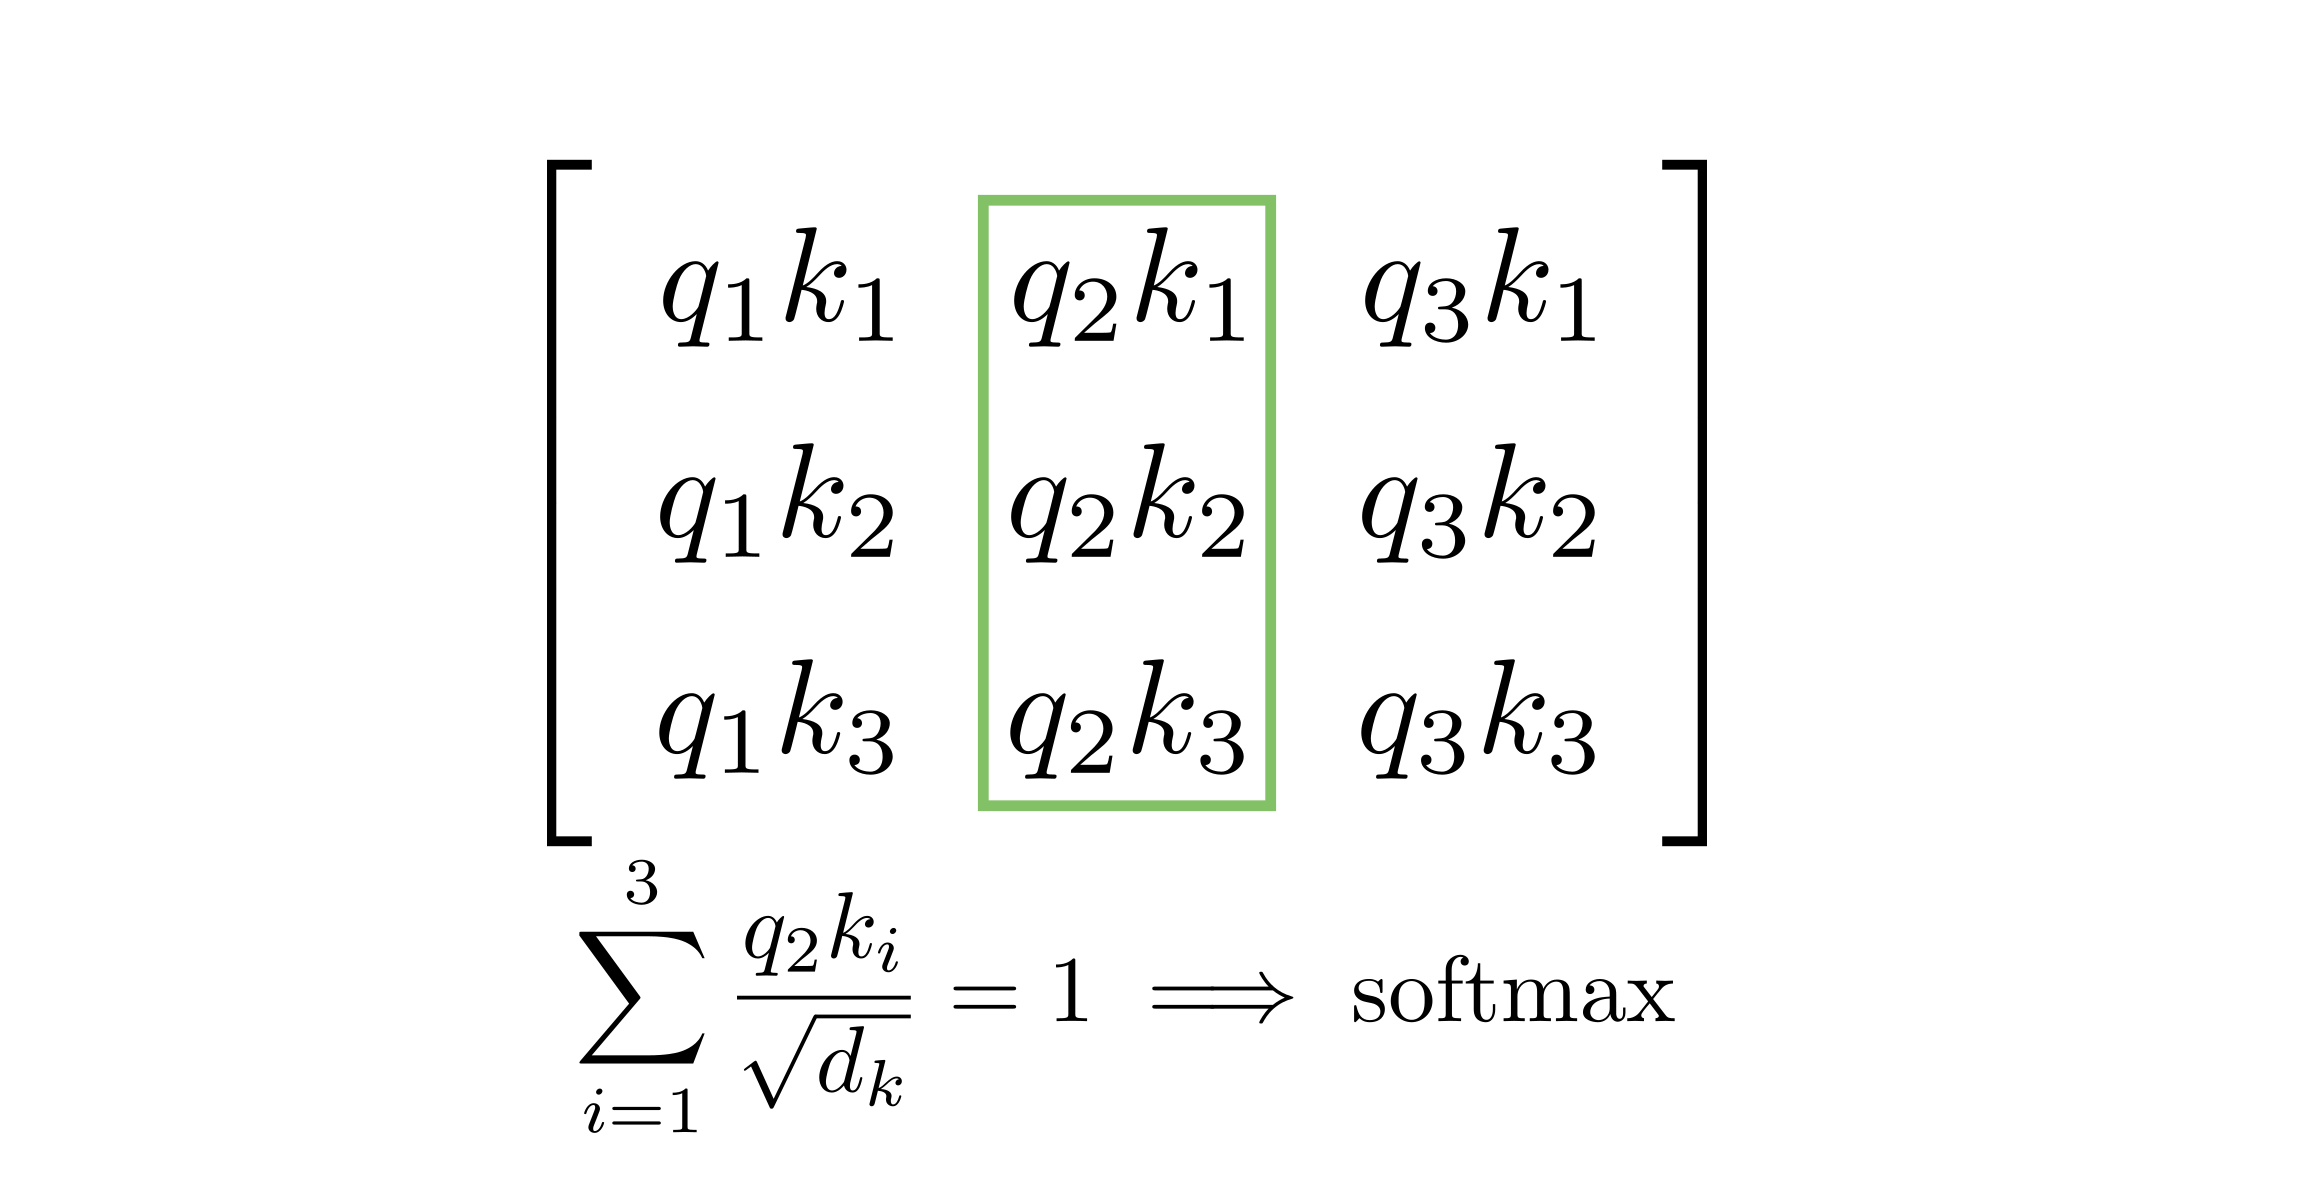
\includegraphics[width=0.75\linewidth]{figures/04_transformer/Attentionpattern.png}
    \caption{Visualization of scaled dot-product attention. Each row corresponds to a query vector $\mathbf{q}_i^{\intercal}$ and each column to a key vector $\mathbf{k}_j$. The boxed row shows attention weights from query $\mathbf{q}_2$ to all keys. These are normalized via softmax and used to compute a weighted sum over value vectors $\mathbf{v}_j$. Figure created with~\cite{the_manim_community_developers_manim_2025}.}
    \label{fig:Scaled_dot_product}
\end{figure}

In Transformer models, keys, queries, and values are computed as linear projections of the same input embeddings $\mathbf{x}_n$ using learned weight matrices:

\begin{align}
\label{eq:attn_keys}
	\mathbf{k}_n & = \mathbf{W_K} \, \mathbf{x}_n \qquad \mathbf{W_K} \in \mathbb{R}^{d_k \times d_{\mathrm{emb}}} \\
\label{eq:attn_values}
	\mathbf{v}_n & = \mathbf{W_V} \, \mathbf{x}_n \qquad \mathbf{W_V} \in \mathbb{R}^{d_{\mathrm{emb}} \times d_{\mathrm{emb}}} \\
\label{eq:attn_queries}
	\mathbf{q}_n & = \mathbf{W_Q} \, \mathbf{x}_n \qquad \mathbf{W_Q} \in \mathbb{R}^{d_q \times d_{\mathrm{emb}}} 
\end{align}

Because all three vectors are derived from the same embedding, this is referred to as self-attention:


\begin{equation}
\label{eq:self_attention}
	\mathrm{SelfAttn}[\mathbf{x}_n] = \sum_{m=1}^N \alpha \left[ \mathbf{x}_m, \mathbf{x}_n \right] \, \mathbf{v}_m \,.
\end{equation}

In practice, we vectorize the computation by stacking all embeddings into a matrix $\mathbf{X} \in \mathbb{R}^{d_{\mathrm{emb}} \times N}$, with each column $\mathbf{x}_n$ representing a token~\cite{zhang_dive_2023, prince_understanding_2023}. The keys, queries, and values are then computed in matrix form: 

\begin{align}
\label{eq:attn_queries_matrix}
	\mathbf{Q} & = \mathbf{W_Q} \, \mathbf{X} \qquad \mathbf{Q} \in \mathbb{R}^{d_k \times N} \\
\label{eq:attn_keys_matrix}
	\mathbf{K} & = \mathbf{W_K} \, \mathbf{X} \qquad \mathbf{K} \in \mathbb{R}^{d_k \times N} 
\end{align}

The self-attention can then be calculated compactly as:

\begin{align}
\label{eq:self_attn_matrix}
	\mathrm{SelfAttn}[\mathbf{Q}, \mathbf{K}, \mathbf{V}] =  \mathrm{softmax} \left( \frac{\mathbf{Q} \cdot \mathbf{K}^{\intercal}}{\sqrt{d_k} } \right) \mathbf{V} \,.
\end{align}

Instead of using a single attention mechanism, Transformers apply multi-head attention, where $h$ attention heads run in parallel. Each head computes its own self-attention using separate learned projections. The outputs of all heads are concatenated and linearly transformed:

\begin{equation}
\label{eq:multi_head_attn}
	\mathrm{MultiHeadSelfAttn}[\mathbf{X}] = \mathbf{W_C} \begin{pmatrix} \mathrm{SelfAttn}^{1}[\mathbf{X}] \\
	\vdots \\
	\mathrm{SelfAttn}^{h}[\mathbf{X}] \end{pmatrix} \qquad \mathbf{W_C} \in \mathbb{R}^{d_k \times d_k}
\end{equation}

The final projection matrix $\mathbf{W_C}$ ensures that the concatenated output has the same shape as the original input $\mathbf{X}$. A typical and efficient choice is to set $d_k = d_{\mathrm{emb}}/h$ so that the total output dimension matches the embedding dimension~\cite{zhang_dive_2023, prince_understanding_2023, murphy_probabilistic_2022}. 


\subsubsection{Transformer architecture for LEGEND waveforms}\label{sec:04_transformer_used}

Let us now consider the specific Transformer model used in this work. It was implemented by Marta Babicz in Python using the Pytorch framework~\cite{ansel_pytorch_2024}. The architecture is encoder-only and closely resembles BERT (Bidirectional Encoder Representations from Transformers), originally introduced by Google~\cite{devlin_bert_2019}.


The input data consists of physical waveforms recorded by the LEGEND-200 experiment. Each waveform spans $20.4 \;\mu$s sampled at 1400 time steps. These waveforms are segmented into $n_t = 140$ tokens, each representing 10 time steps, and embedded into a vector of size $d_{\mathrm{emb}} = 128$. After tokenization and embedding, positional encoding is added as described in section~\ref{sec:03_input_representation}. 
The model contains $n_l = 6$ encoder layers, each using 8 attention heads in parallel. Each attention block and feedforward block is wrapped in a residual connection and followed by layer normalization, following the original Transformer design. 
Altogether, the network has nearly 1.2 million trainable parameters. Roughly one-third of these lie in the attention layers, while two-thirds are trained in the feedforward network. Table~\ref{tab:model_parameters} gives a detailed parameter breakdown. 

For the task at hand -- namely analyzing long-sequence waveform data -- Transformers are particularly well suited. Convolutional neural networks and Recurrent neural networks are generally limited in capturing long-range dependencies due to their fixed receptive fields or sequential processing. By contrast, multi-head attention can focus on multiple regions of the waveform simultaneously, enabling the model to learn subtle temporal patterns beyond classical features such as A/E. The Transformer's ability to model global context, apply dynamic attention, and process sequences in parallel is particularly valuable for pulse-shape analysis. The waveforms encode rich spatial and temporal information about energy depositions in the detector, with features that range across the full waveform. 
In the following chapter, we describe how this Transformer model was trained and evaluated on waveform data, including dataset preparation, model configuration, and training procedures. 


\begin{table}[t]
\centering
\caption{Overview of the trainable parameters of the Transformer model used in this work.  The dimension of the embedding is $d_{\mathrm{emb}} = 128$, which is equal to the dimension of the keys and queries. The number of encoder layers is $n_{l} = 6$, the number of labels $n_{\mathrm{labels}} = 4$, and the number of neurons in the feedforward network $n_n = 512$. The factor 2 in the embedding comes from the fact that we embed not only the waveform but also the gradients.} 
\label{tab:model_parameters}
\begin{tabular}{|c | c | c | c|}
	\hline
	\textbf{Architecture} & \textbf{Weights} & \textbf{Bias} & \textbf{Parameters} \\
 	\hline
 	Tokenization & $d_{\mathrm {emb}}$  & - &  128 \\
 	\hline
 	Embedding & $2 \times 10 \times d_{\mathrm{emb}}$ & $2 \times d_{\mathrm{emb}}$ & 2816 \\
 	\hline
 	Keys  & $d_{\mathrm{emb}} \times d_{\mathrm{emb}} \times n_{l}$ & $d_{\mathrm{emb}} \times n_{l}$ &  99072 \\
 	\hline
   	Queries & $d_{\mathrm{emb}} \times d_{\mathrm{emb}} \times n_{l}$ & $d_{\mathrm{emb}} \times n_{l} $ & 99072 \\
 	\hline
 	Values & $d_{\mathrm{emb}} \times d_{\mathrm{emb}} \times n_{l}$ & $d_{\mathrm{emb}} \times n_{l}$ & 99072 \\
 	\hline
 	Output matrix & $d_{\mathrm{emb}} \times d_{\mathrm{emb}} \times n_{l}$ & $d_{\mathrm{emb}} \times n_{l}$ & 99072 \\
 	\hline
 	Linear layer 1 & $d_{\mathrm{emb}} \times n_{n} \times n_{l}$ & $n_{n} \times n_{l}$ & 396288 \\ 
 	\hline
	Linear layer 2 & $n_{n} \times d_{\mathrm{emb}} \times n_{l}$ & $d_{\mathrm{emb}} \times n_{l}$ & 393984 \\
	\hline
	Normalization 1 & $d_{\mathrm{emb}} \times n_{l}$ & $d_{\mathrm{emb}} \times n_{l}$ & 1536 \\
	\hline
	Normalization 2 & $d_{\mathrm{emb}} \times n_{l}$ & $d_{\mathrm{emb}} \times n_{l}$ & 1536 \\
	\hline
	Decoder & $n_{\mathrm{labels}} \times d_{\mathrm{emb}}$ & $n_{\mathrm{labels}}$ & 516 \\
	\hline
	De-embedding & $2 \times d_{\mathrm{emb}}$ & - & 256 \\
	\hline
	Total: & & & 1193348 \\
	\hline
\end{tabular}
\end{table}





%--------------------- PSD with Transformers ---------------------
\clearpage
\section{Pulse shape discrimination with Transformers} 
\markboth{PSD with Transformers}{PSD with Transformers}
\label{sec:05_PSD_efficiency}
Having introduced the theoretical foundations of machine learning and the specific architecture of the Transformer model used in this work, we now turn to their practical implementation in the context of this work. 
This chapter begins by outlining the structure and organization of waveform data in the LEGEND-200 experiment. We then describe the procedure for constructing training datasets, which includes data selection and data cleaning. 
The different models developed in this work are presented alongside their classification performance. We continue with a brief overview of the pulse shape simulation (PSS) framework in LEGEND-200, and conclude this chapter by summarizing key results. 


\subsection{Data in the LEGEND-200 experiment} \label{sec:04_LEGEND_data}

The DAQ process in LEGEND-200 follows a structured hierarchy to ensure consistency across the dataset. Each DAQ cycle -- a continuous block of data-taking, synchronously started and stopped by the DAQ system -- is stored as a separate file and marked with a GPS timestamp.  
A sequence of DAQ cycles recorded under a consistent detector configuration is grouped into a run. Each run begins with a series of calibration cycles, followed by physics cycles. 
Runs are then grouped into larger units called periods, which are separated by major changes in the detector setup or operating conditions that could impact analysis results. 
However, not all periods and runs are suitable for physics analysis. Only a subset has passed the data quality checks established by the collaboration~\cite{lnote_24010}. Table~\ref{tab:periods_runs} summarizes all physics runs that were deemed usable for this work.

\begin{table}[b]
\centering
\caption{Summary of all physics runs that passed the LEGEND quality checks~\cite{lnote_24010}, including live time and total exposure (ICPC detectors only). } 
\begin{tabular}{||c | c | c| c | c||} 
    \hline
    \textbf{Period} & \textbf{Runs} & \textbf{Start date} & \textbf{Live time [yr]}  & \textbf{Exposure [kg$\cdot$yr]} \\ 
    \hline
    3 & 0-5 & 2023-03-12 & 0.08 & 4.85 \\
    \hline
    4 & 0-3 & 2023-04-15 & 0.047 & 2.89 \\
    \hline
    6 & 0-5 & 2023-06-11 & 0.110 & 6.68 \\
    \hline
    7 & 2-7 & 2023-07-31 & 0.096 & 5.82 \\
    \hline
    8 & 0-4, 6-14 & 2023-10-03 & 0.237 & 14.39 \\
    \hline
    9 & 0-5 & 2024-01-11 & 0.093 & 5.67 \\
    \hline
\end{tabular}
\label{tab:periods_runs}
\end{table}

The raw waveforms recorded by the LEGEND-200 experiment are stored at NERSC in HDF5 (Hierarchical Data Format version 5). HDF5 is a binary file format designed to store and organize large, complex datasets. It is well-suited for large datasets because it supports fast I/O and efficient partial data access. Therefore, the entire file need not be loaded into memory. 

The collaboration has developed a sophisticated digital signal processing pipeline. Its initial stage operates directly on the raw waveforms, with subsequent stages performing higher-level processing, as illustrated in figure~\ref{fig:data_flow}. 

In the initial stage, the digitized waveforms recorded by the DAQ system are stored in the RAW (raw waveform and ADC information) tier. This tier also includes metadata such as the timestamp of the recording and the measured energy in ADC units. 
For the DSP (digitally processed features)  tier, each waveform is processed independently to extract signal features. This tier contains several parameters directly derived from the waveform, for example, various energy estimates, amplitude, and baseline. 
The HIT (hit-level calibrated parameters) tier contains parameters derived from a multi-waveform analysis. This includes calibrated energy values, A/E ratios, and LQ cut values. All data tiers up to this point are organized in separate subdirectories and indexed by timestamp, enabling efficient access to specific waveforms. 
In contrast, the EVT (event cluster level) tier clusters individual waveforms into events. Each event may consist of multiple coincident hits in the HPGe detectors, as well as in other subsystems, such as the SiPMs and the muon veto. 
Finally, the TCM (trigger and calibration metadata) tier includes information related to event building, along with data from calibration pulses.


\begin{figure}[t]
    \centering
    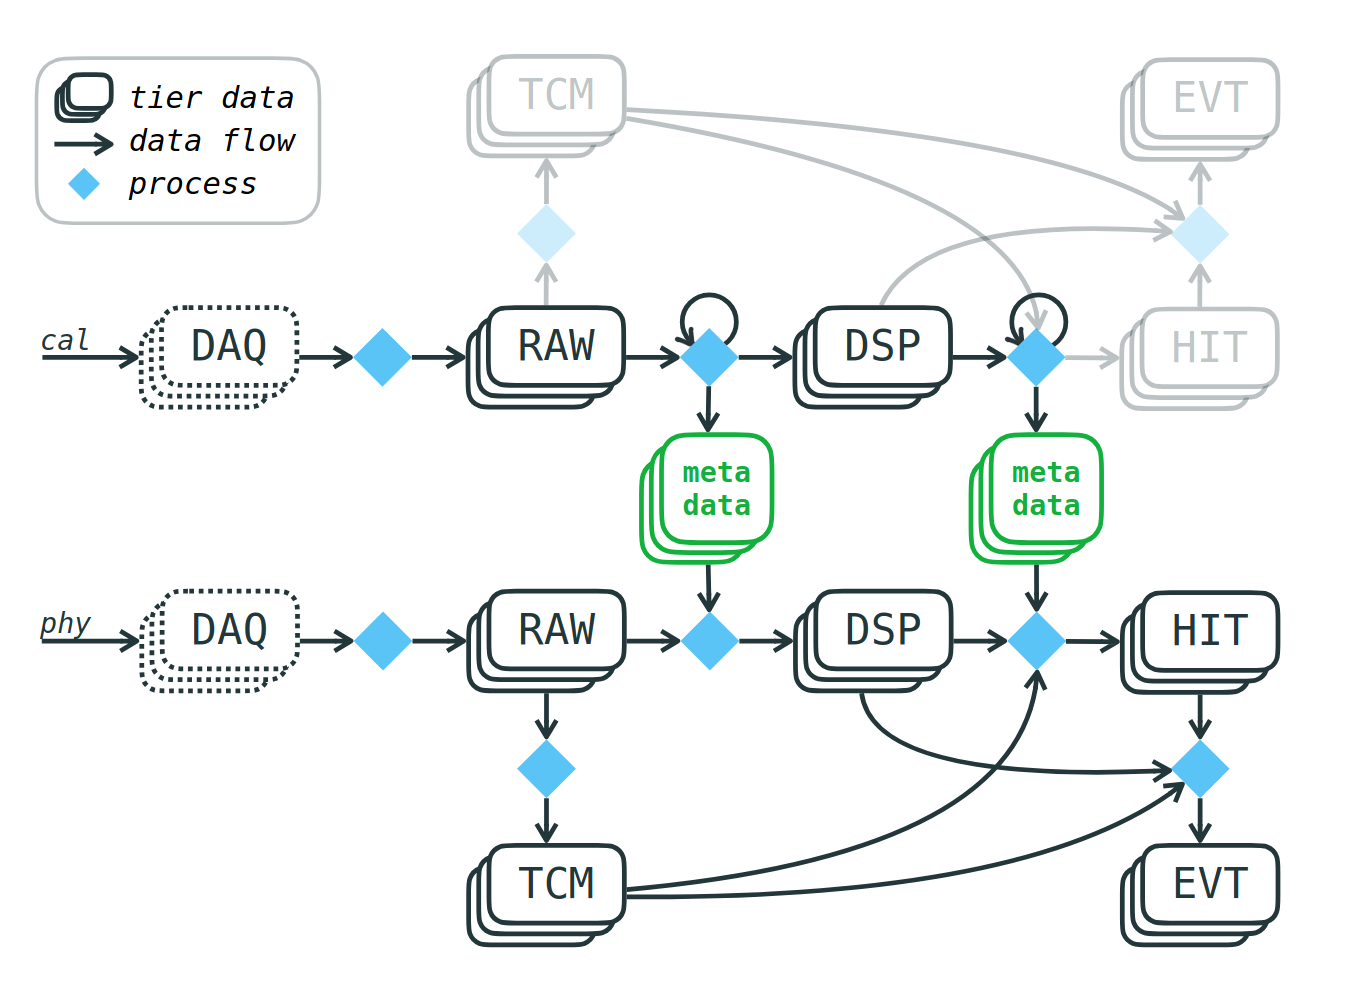
\includegraphics[width=0.85\linewidth]{figures/05_PSD/Data_flow.png}
    \caption{Data flow for the LEGEND-200 experiment. Starting from the DAQ output, the data undergoes multiple processing steps before being clustered into coincident events in the EVT tier. The calibration data, acquired using sources that produce signals at well-known energies, is used to define and validate analysis cuts and to establish a precise energy scale. These calibrations are then applied to the physics data. Image credit to Luigi Pertoldi~\cite{noauthor_pyhep_2023}. } 
\label{fig:data_flow}
\end{figure}


\subsection{Data preparation for Transformer training}

In supervised machine learning, the quality of the training data is critical. The performance of a model is fundamentally limited by the cleanliness and reliability of the dataset it is trained on. 

To address this, we developed a code framework that combines waveforms and processing parameters from multiple data tiers into a unified dataset suitable for training machine learning models. Each waveform is then classified (labeled) according to the established LEGEND-200 analysis methods. 

The dataset is subsequently cleaned to maximize class purity and minimize contamination from misclassified events. The impact of this data-cleaning procedure is illustrated in figure~\ref{fig:datacleaning_fullspectrum}, where we show data from period 3 (only ICPC detectors).

\begin{figure}[t]
    \centering
    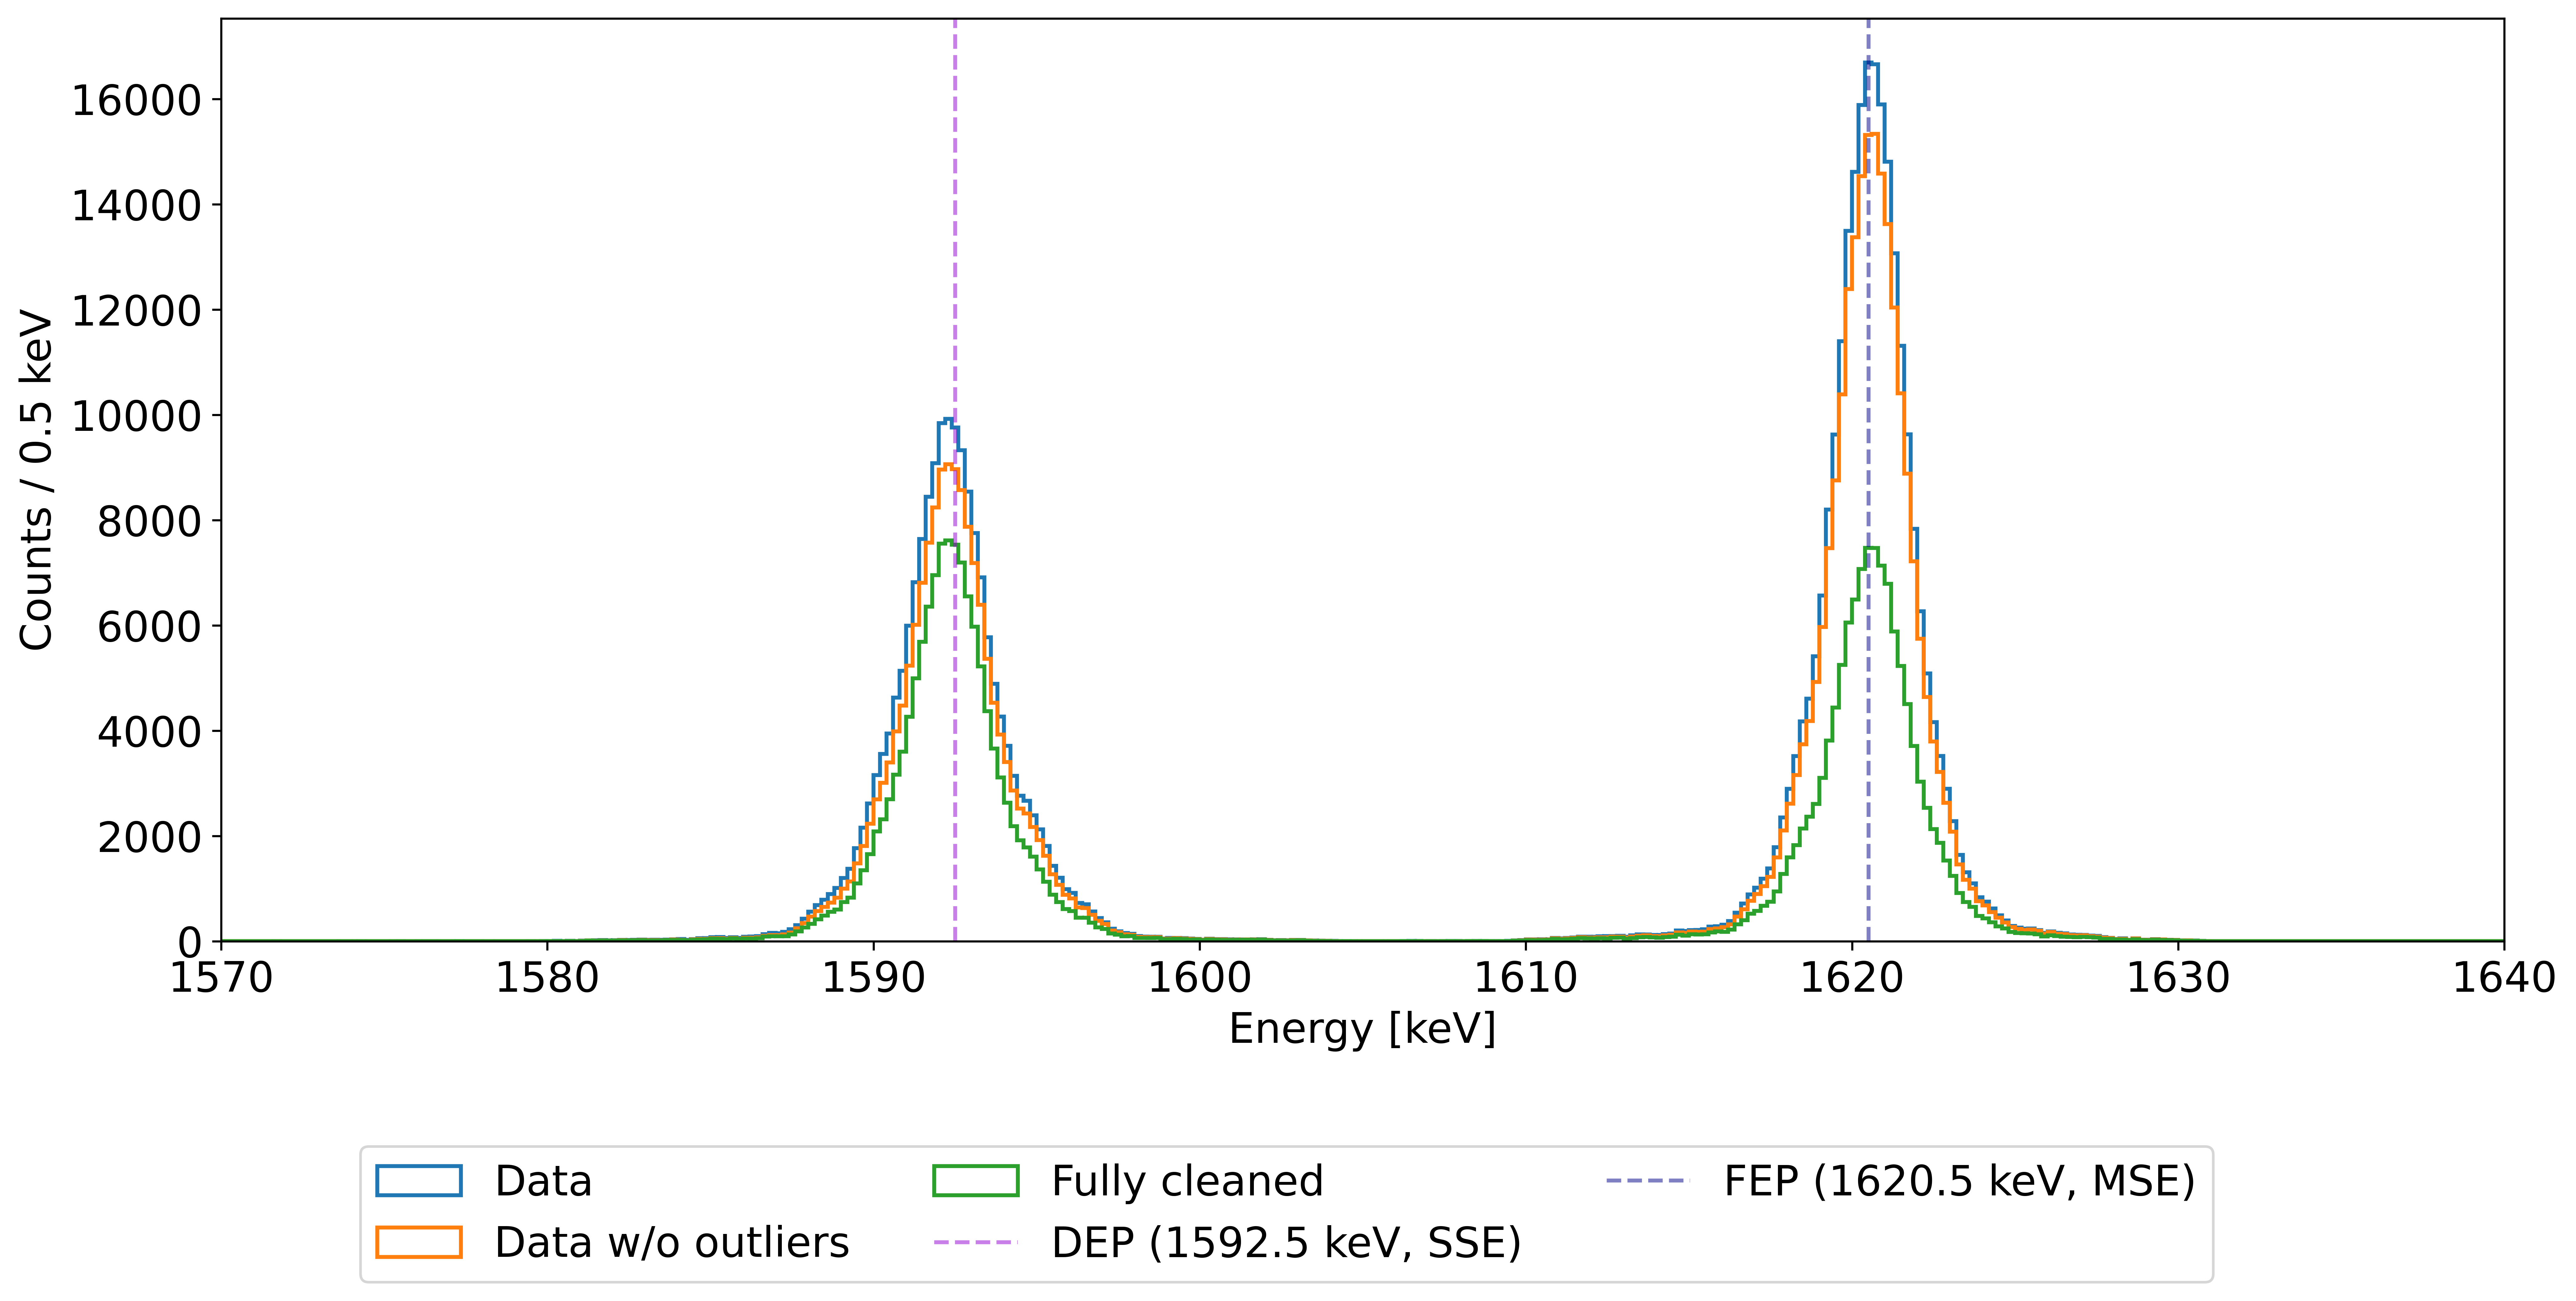
\includegraphics[width=\linewidth]{figures/05_PSD/Data_cleaning_fullspectrum.png}
    \caption{Effect of the data cleaning procedure on two pre-selected peaks ($\pm 3\, \sigma$) from the $^{228}$Th calibration in period 3, using only ICPC detectors. The plot shows the impact of the two cleaning steps applied to pre-selected data (blue): removal of statistical outliers (orange) and exclusion of events with non-matching numbers of peaks in the gradient waveforms (green, combined effect). The latter has a strong impact on the full energy peak, as expected, since SSEs are already very pure, while the MSE class tends to be heterogeneous.} 
\label{fig:datacleaning_fullspectrum}
\end{figure}


\subsubsection{Data selection}

The data selection begins by loading the calibrated energies from the HIT tier. In this work, we use the energy estimated with the trapezoid filter (explained in section~\ref{sec:HPGe_legend}). The HDF5 files, which have a specific structure, are accessed with \textit{legend-pydataobj}, a package that provides a Python implementation of the LEGEND Data Objects to HDF5~\cite{detwiler_legend-pydataobj_2025}. Detector metadata is used to select only detectors that were active and functioning properly during data taking. 

For events falling within a specified energy range, the corresponding indices are stored for further processing. For datasets intended for training, the algorithm automatically selects a $ \pm 3 \,\sigma$ window around the four prominent calibration peaks in the $^{228}$Th spectrum. 
This window is estimated from the FWHM of the energy resolution. Alternatively, a custom energy window can be manually defined, for example, to load a continuous dataset for benchmarking the Transformer model against conventional PSD methods. 
Once the energy range is specified, waveforms are loaded from the RAW tier by indexing the file location within the subdirectory structure. Throughout this work, we use waveforms windowed around the rising edge, sampled 1400 times at 16~ns intervals. 
Pre-selecting events in the HIT tier significantly reduces runtime by up to two orders of magnitude, since only waveforms in the relevant energy range are loaded. These energy windows typically span tens of keV and represent only a small fraction of the total dataset. 

We then apply quality cuts to remove waveforms that deviate from expected detector response characteristics. For this purpose, we apply the same set of quality cuts developed and validated for the LEGEND-200 physics analyses, which are defined in~\cite{lnote_24011}. We remove all waveforms that contain:

\begin{itemize}
    \item discharges (is\_delayed\_discharge)
    \item unstable baselines (is\_valid\_bl\_slope, is\_valid\_bl\_slope\_rms)
    \item noisy tails (is\_valid\_tail\_rms)
    \item noise bursts in the rising edge (is\_not\_noise\_burst)
    \item invalid energies (is\_valid\_cuspEmax, is\_valid\_cuspEmin, is\_low\_cuspEmax)
    \item invalid trap filter (is\_valid\_trap\_tpmin, is\_valid\_trap\_tpmax)
    \item invalid rise times (is\_valid\_t0, is\_valid\_rt, is\_valid\_dteff)
\end{itemize}

In the final step of the data selection, the remaining events are classified.
As discussed in section~\ref{sec:02_PSD} and shown in figure~\ref{fig:PSD_topology}, the amplitude-to-energy ratio is particularly well suited for distinguishing different event topologies. Table~\ref{tab:event_classification} summarizes the classification scheme. 

The resulting dataset consists of waveforms within the desired energy range that have been classified accordingly. While the class labels are already very pure, the events within each class still exhibit a degree of heterogeneity that will affect model training. 

\begin{table}
\centering
\caption{Analytical labels for the waveforms, based on the LEGEND-200 analysis. The most important component is the A/E parameter. For ICPC detectors produced by Mirion Technologies, the LQ cut is not applied because it is not reliable.} 
\begin{tabular}{||c | c | c||} 
 \hline
 \textbf{Label} & \textbf{A/E value} & \textbf{LQ value} \\ 
 \hline
 SSE & intermediate & low \\ 
 \hline
 MSE & low & - \\ 
 \hline
 p-contact & high & - \\ 
 \hline
 n-contact & low & high \\ 
 \hline
\end{tabular}
\label{tab:event_classification}
\end{table}

\subsubsection{Data cleaning}

In the second stage of the data preparation, the dataset is further cleaned to increase the purity of the class labels. Two methods are applied: peak estimation and outlier removal. 
For peak estimation, the derivative of each waveform is computed. To increase the robustness of the peak identification, the gradients are smoothed using a rolling window with a Gaussian kernel (applied over 5 timestamps with a width of $1.5 \,\sigma$). The resulting derivative signal is then normalized to reduce energy dependence. 



To identify distinct signal components in the derivative waveform, we used the \textit{find\_peaks} function from the scipy module~\cite{virtanen_scipy_2020}, which allows for peak detection based on height and prominence. An example of single-site and multi-site peak identification is shown in figure~\ref{fig:datacleaning_PeakID}. 
For waveforms labeled as MSE, multiple peaks are required, as this corresponds to multiple time-separated charge drifts within a germanium diode. For all other event categories, only a single peak per waveform is permitted. 
Note that the labels of the waveforms are not changed during this process; instead, waveforms that do not meet the peak criteria are simply rejected. This cleaning cut is very strict, and removes more than half of the events ($51.2~\%$, benchmarked on period 3). In this step, we also extract the FWHM of the largest peak, which is used for outlier rejection.

\begin{figure}[t]
    \centering
    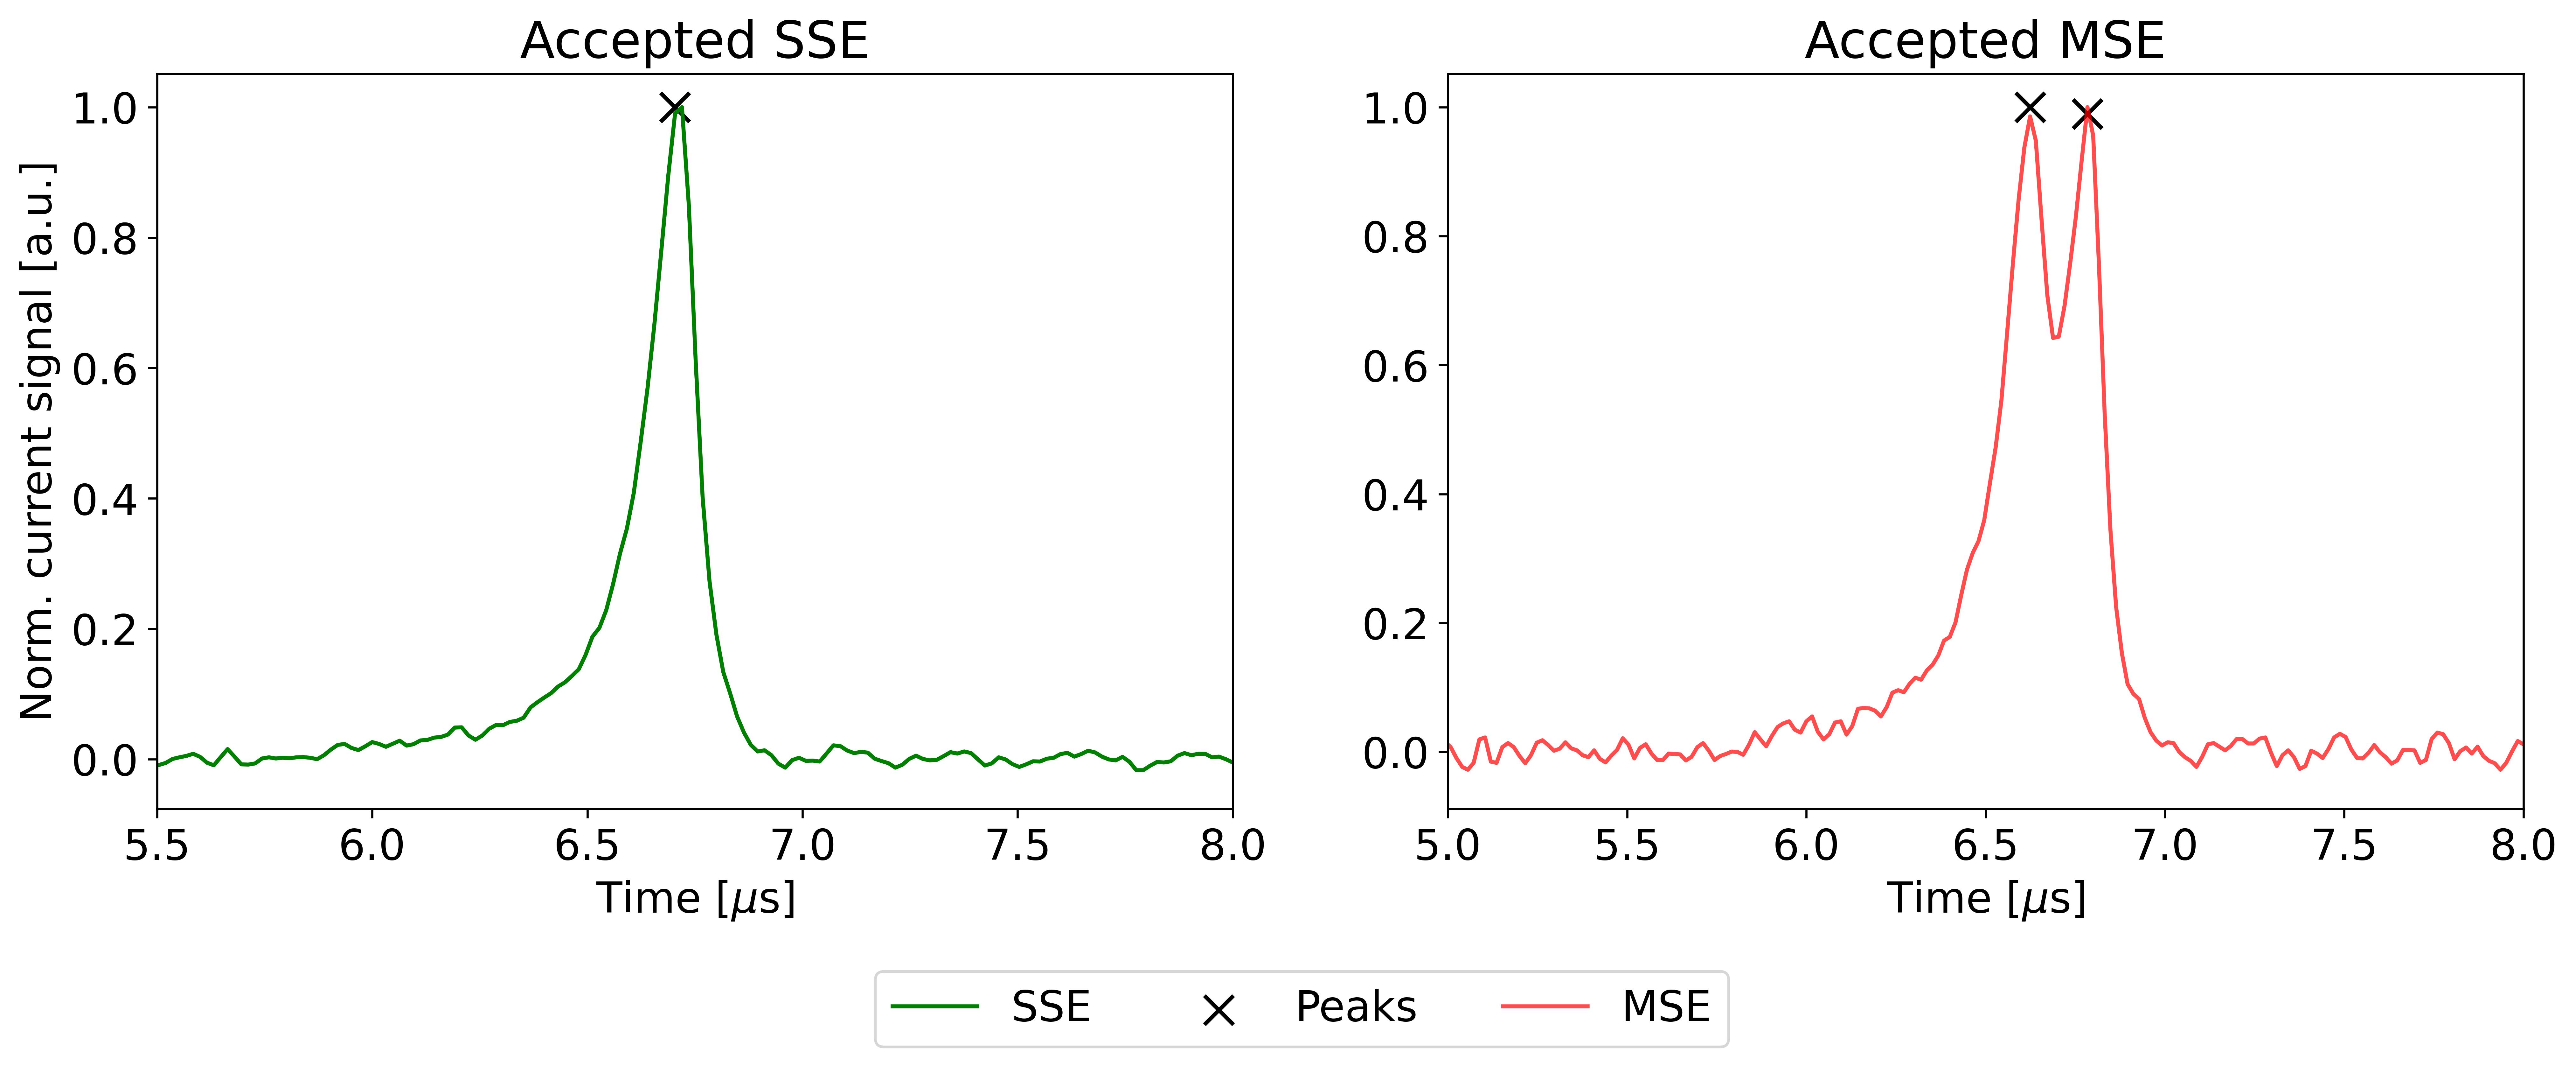
\includegraphics[width=\linewidth]{figures/05_PSD/Plot_DataCleaning_PeakID_V02160A.png}
    \caption{Peak identification for ICPC detector V02160A during period 3. The left panel shows a single-site event with one identified peak; the right panel shows a multi-site event with multiple peaks. Both are accepted.}
\label{fig:datacleaning_PeakID}
\end{figure}

\begin{table}
\centering
\caption{Parameters where outliers are removed in the data cleaning procedure. Generally, only a few events are removed in each cut ($< 3\%$). Efficiency values are determined from data taken during period 3. The total efficiency is obtained by applying all cuts simultaneously and is smaller than the product of individual efficiencies, as some waveforms fail multiple cuts. }
\begin{tabular}{||c | c | c | c |c ||} 
 \hline
 \textbf{Quantity} & \textbf{Description} & \textbf{Range} & \textbf{Cut Eff.} [\%] \\ 
 \hline
 tp-10 & Time where $A$ reaches 10 \%  	& $3 \,\sigma$ & 97.7\\ 
 \hline
 tp-50 & Time where $A$ reaches 50 \% 	& $3 \,\sigma$ & 98.0 \\ 
 \hline
 tp-80 & Time where $A$ reaches 80 \% 	& $3 \,\sigma$ & 97.8 \\
 \hline
 rt1 & Time between tp-10 and tp-90 				& $3 \,\sigma$ & 97.8 \\
 \hline
 rt2 & Time between tp-10 and tp-50 				& $3 \,\sigma$ & 97.6 \\ 
 \hline
 AoE & Area divided by energy & $3 \,\sigma$ & 99.0 \\
 \hline
 LQ & Measure for the late charge 			& $3 \,\sigma$ & 99.1 \\
 \hline
 Peak width & FWHM of the largest peak 		& $2 \,\sigma$ & 98.0 \\
 \hline
 \textbf{Total} & All cleaning cuts applied & - & 91.9 \\
 \hline
\end{tabular}
\label{tab:Data_cleaning_param}
\end{table}

To identify outliers, we calculate the mean and standard deviation of all parameters listed in table~\ref{tab:Data_cleaning_param}, separately for each detector and label. Waveforms with a peak FWHM outside a $ \pm 3 \,\sigma$ window are rejected -- except for MSE events, where we apply only a lower-bound cut. 
This exception accounts for cases where two nearby peaks merge slightly, causing the FWHM of the dominant peak to broaden. Such events are not rejected to preserve valid MSE samples. 

\begin{figure}[t]
    \centering
    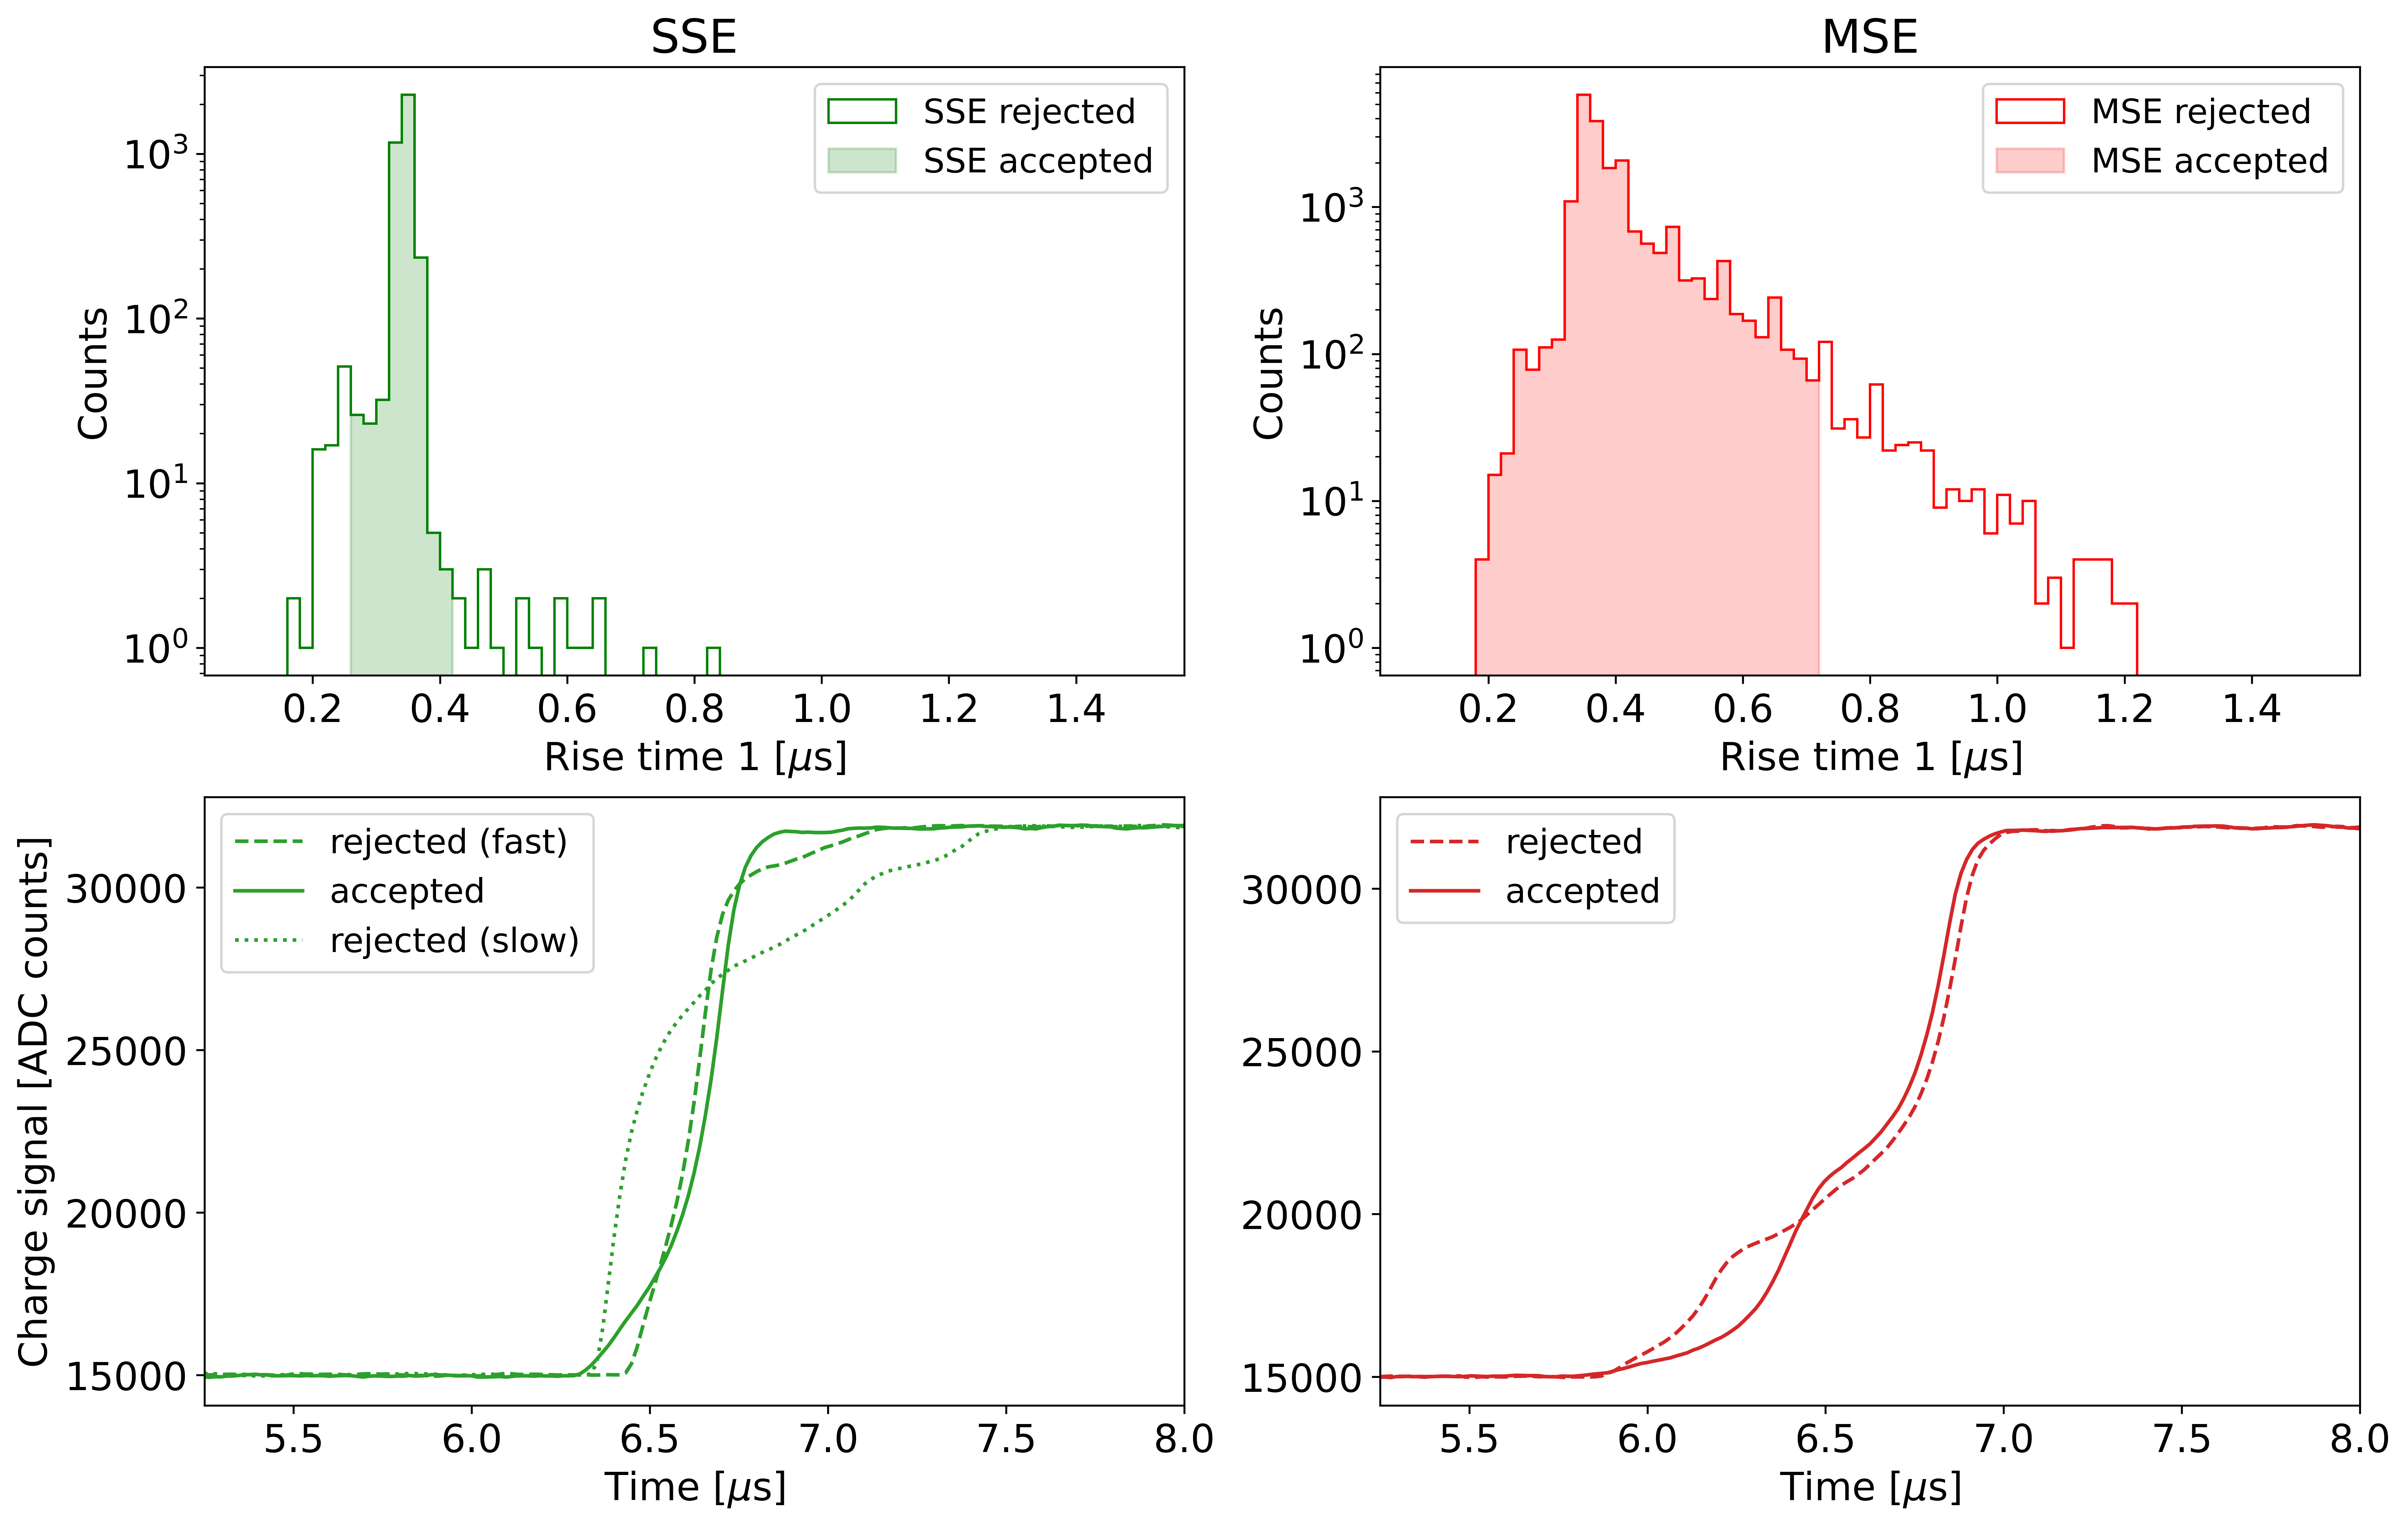
\includegraphics[width=\linewidth]{figures/05_PSD/Plot_DataCleaning_rt1_V02160A.png}
    \caption{Rise time outlier removal ($3 \, \sigma$) for ICPC detector V02160A during period 3. The top panels show histograms of accepted and rejected events; the bottom panels show example waveforms. Single-site events (left) are more homogeneous than multi-site events (right). In the bottom left, an accepted waveform (solid) is compared to outliers with too fast (dashed) and too slow (dotted) rise times. Similar rejection is applied to long-rise-time MSE events (bottom right).}
    \label{fig:datacleaning_rt1}
\end{figure}

For the other quantities described in table~\ref{tab:Data_cleaning_param}, a symmetric $ \pm 2 \, \sigma$ window is applied for outlier rejection. In total, around 8\% of events are rejected in this step. Outlier removal is illustrated in figure~\ref{fig:datacleaning_rt1}, which shows rise time cleaning cuts for single-site and multi-site events, and in figure~\ref{fig:datacleaning_fwhm}, which shows cuts on the FWHM of the peak with the highest amplitude. Both figures include example waveforms of accepted and rejected events. 



\begin{figure}
    \centering
    \includegraphics[width=\linewidth]{figures/05_PSD/Plot_DataCleaning_fwhm_V02160A.png}
    \caption{Peak width outlier removal ($2 \, \sigma$) for ICPC detector V02160A during period 3. The top panels show histograms of accepted and rejected events; the bottom panels show example differentiated waveforms. For multi-site events, only a lower peak width bound is applied to avoid rejecting merged peaks. Bottom left: accepted SSE waveform (solid) vs. rejected broadened peak (dashed). Bottom right: rejected waveform (dashed) with a sharp rise, indicating interaction near the p$^{+}$ electrode.}
    \label{fig:datacleaning_fwhm}
\end{figure}

\subsection{Model training and evaluation}

The Transformer model architecture used in this work is described in section~\ref{sec:04_transformer_used}. It was trained on several datasets, each prepared according to the procedures outlined in the previous subsections. An overview of all datasets used for training is provided in table~\ref{tab:Datasets_overview}. 
The models are trained using four NVIDIA V100 GPUs on the Perlmutter supercomputer at the National Energy Research Scientific Computing Center (NERSC) in Berkeley, California. 
The datasets were split into three parts: 60\% for training (used to optimize model weights), 10\% for validation (used to monitor generalization performance and prevent overfitting), and 30\% for testing. The validation set allows for early stopping, terminating training when the validation loss is no longer improving, and performance monitoring without influencing the model's parameters. 
Since its purpose is monitoring, a relatively small share is sufficient. The test set is strictly held out and used only to report the final model performance; it must be large enough to provide statistically meaningful results without excessively reducing the training data. 
We used a batch size of 512 per GPU, resulting in an effective batch size of 2048.
The loss function used in this work is the combined loss shown in equation~\refeq{eq:combined_loss}. It is optimized using ADAM, described at the end of section~\ref{sec:03_optimization_algorithms}.  

The different models are then evaluated and assessed with several metrics. 
The precision score, defined in equation~\refeq{eq:precision_score}, measures the proportion of correctly identified positive instances among all instances classified as positive. In the context of single-site events, it quantifies the fraction of events classified as SSE that are truly single-site. A high precision score indicates a low number of false positives.

\begin{equation}
\label{eq:precision_score}
	\mathrm{Precision} = \frac{\mathrm{True \; Positive}}{\mathrm{True \; Positive + False \; Positive}} \,. 
\end{equation}

Sensitivity addresses the complementary aspect by quantifying the proportion of true SSE events that are correctly identified. A high sensitivity indicates a low number of false negatives, meaning the model effectively captures most of the true positive cases: 

\begin{equation}
\label{eq:sensitivity_score}
	\mathrm{Sensitivity} = \frac{\mathrm{True \; Positive}}{\mathrm{True \; Positive + False \; Negative}} \,.
\end{equation}

In machine learning, the F1-score is commonly reported alongside precision and sensitivity as a measure of the balance between the two:

\begin{equation}
\label{eq:f1_score}
	\mathrm{F_1} = 2 \; \frac{\mathrm{Precision} \cdot \mathrm{Sensitivity}}{\mathrm{Sensitivity + Precision}} \,.
\end{equation}


A confusion matrix provides a compact graphical representation of classification performance. For $n_{\mathrm{label}}$ classes, it is an $n_{\mathrm{label}} \times n_{\mathrm{label}}$ matrix in which each row corresponds to the ground truth and each column to the model's predicted class. The diagonal entries indicate correct classifications, while the off-diagonal entries represent misclassifications, including false positives and false negatives~\cite{murphy_probabilistic_2022}.  

\begin{table}
\centering
\caption{Datasets used for training the Transformer, only including ICPC detector waveforms. The data size indicates the total number of waveforms in the dataset. In the second Transformer model, $p^{+}$ and $n^{+}$ events are combined into a single surface label.}
\begin{tabular}{||c | c | c | c | c||} 
 \hline
 \textbf{Transformer} & \textbf{Periods} & \textbf{Data size} & \textbf{Isotopes} & \textbf{Labels} \\ 
 \hline
 Model 1 & 3 - 10 & 12.5 $\times 10^6$ & $^{228}$Th & SS, MS, p$^{+}$, n$^{+}$ \\ 
 \hline
 Model 2 & 3 - 11 & 14.0 $\times 10^6$ & $^{228}$Th, $^{56}$Co & SS, MS, surface \\
 \hline
 Model 3 & 3 \& 11 & 3.0 $\times 10^6$ & $^{228}$Th, $^{56}$Co & SS, MS, p$^{+}$, n$^{+}$ \\
 \hline
\end{tabular}
\label{tab:Datasets_overview}
\end{table}


\subsubsection{First Transformer model}

The first model configuration was trained on 12.5 million waveforms extracted from the energy ranges of the four dominant $^{228}$Th calibration peaks. These include the double-escape peak of $^{208}$Tl at 1592.5 keV, the full-energy peak of $^{212}$Bi at 1620.5 keV, and the single-escape and full-energy peaks of $^{208}$Tl at 2103.5 keV and 2614.5 keV, respectively. 
We used waveforms from periods 3 to 10 for this dataset. 

The true labels were assigned according to the classification scheme outlined in table~\ref{tab:event_classification}. The classification performance is illustrated by the confusion matrix in figure~\ref{fig:Confusionmatrix_icpc_v1}, which shows the precision. The corresponding scores are summarized in table~\ref{tab:Scores_icpc_v1}. The model achieves very high precision for both single-site and multi-site events, as well as strong precision for surface event classification. Sensitivity is notably lower for SSE and p$^+$ events in contrast to MSE and n$^+$ events, indicating some degree of cross-contamination between these classes. Despite this, all F1-scores exceed 95\%, demonstrating an overall excellent classification performance.

\begin{figure}
    \centering
    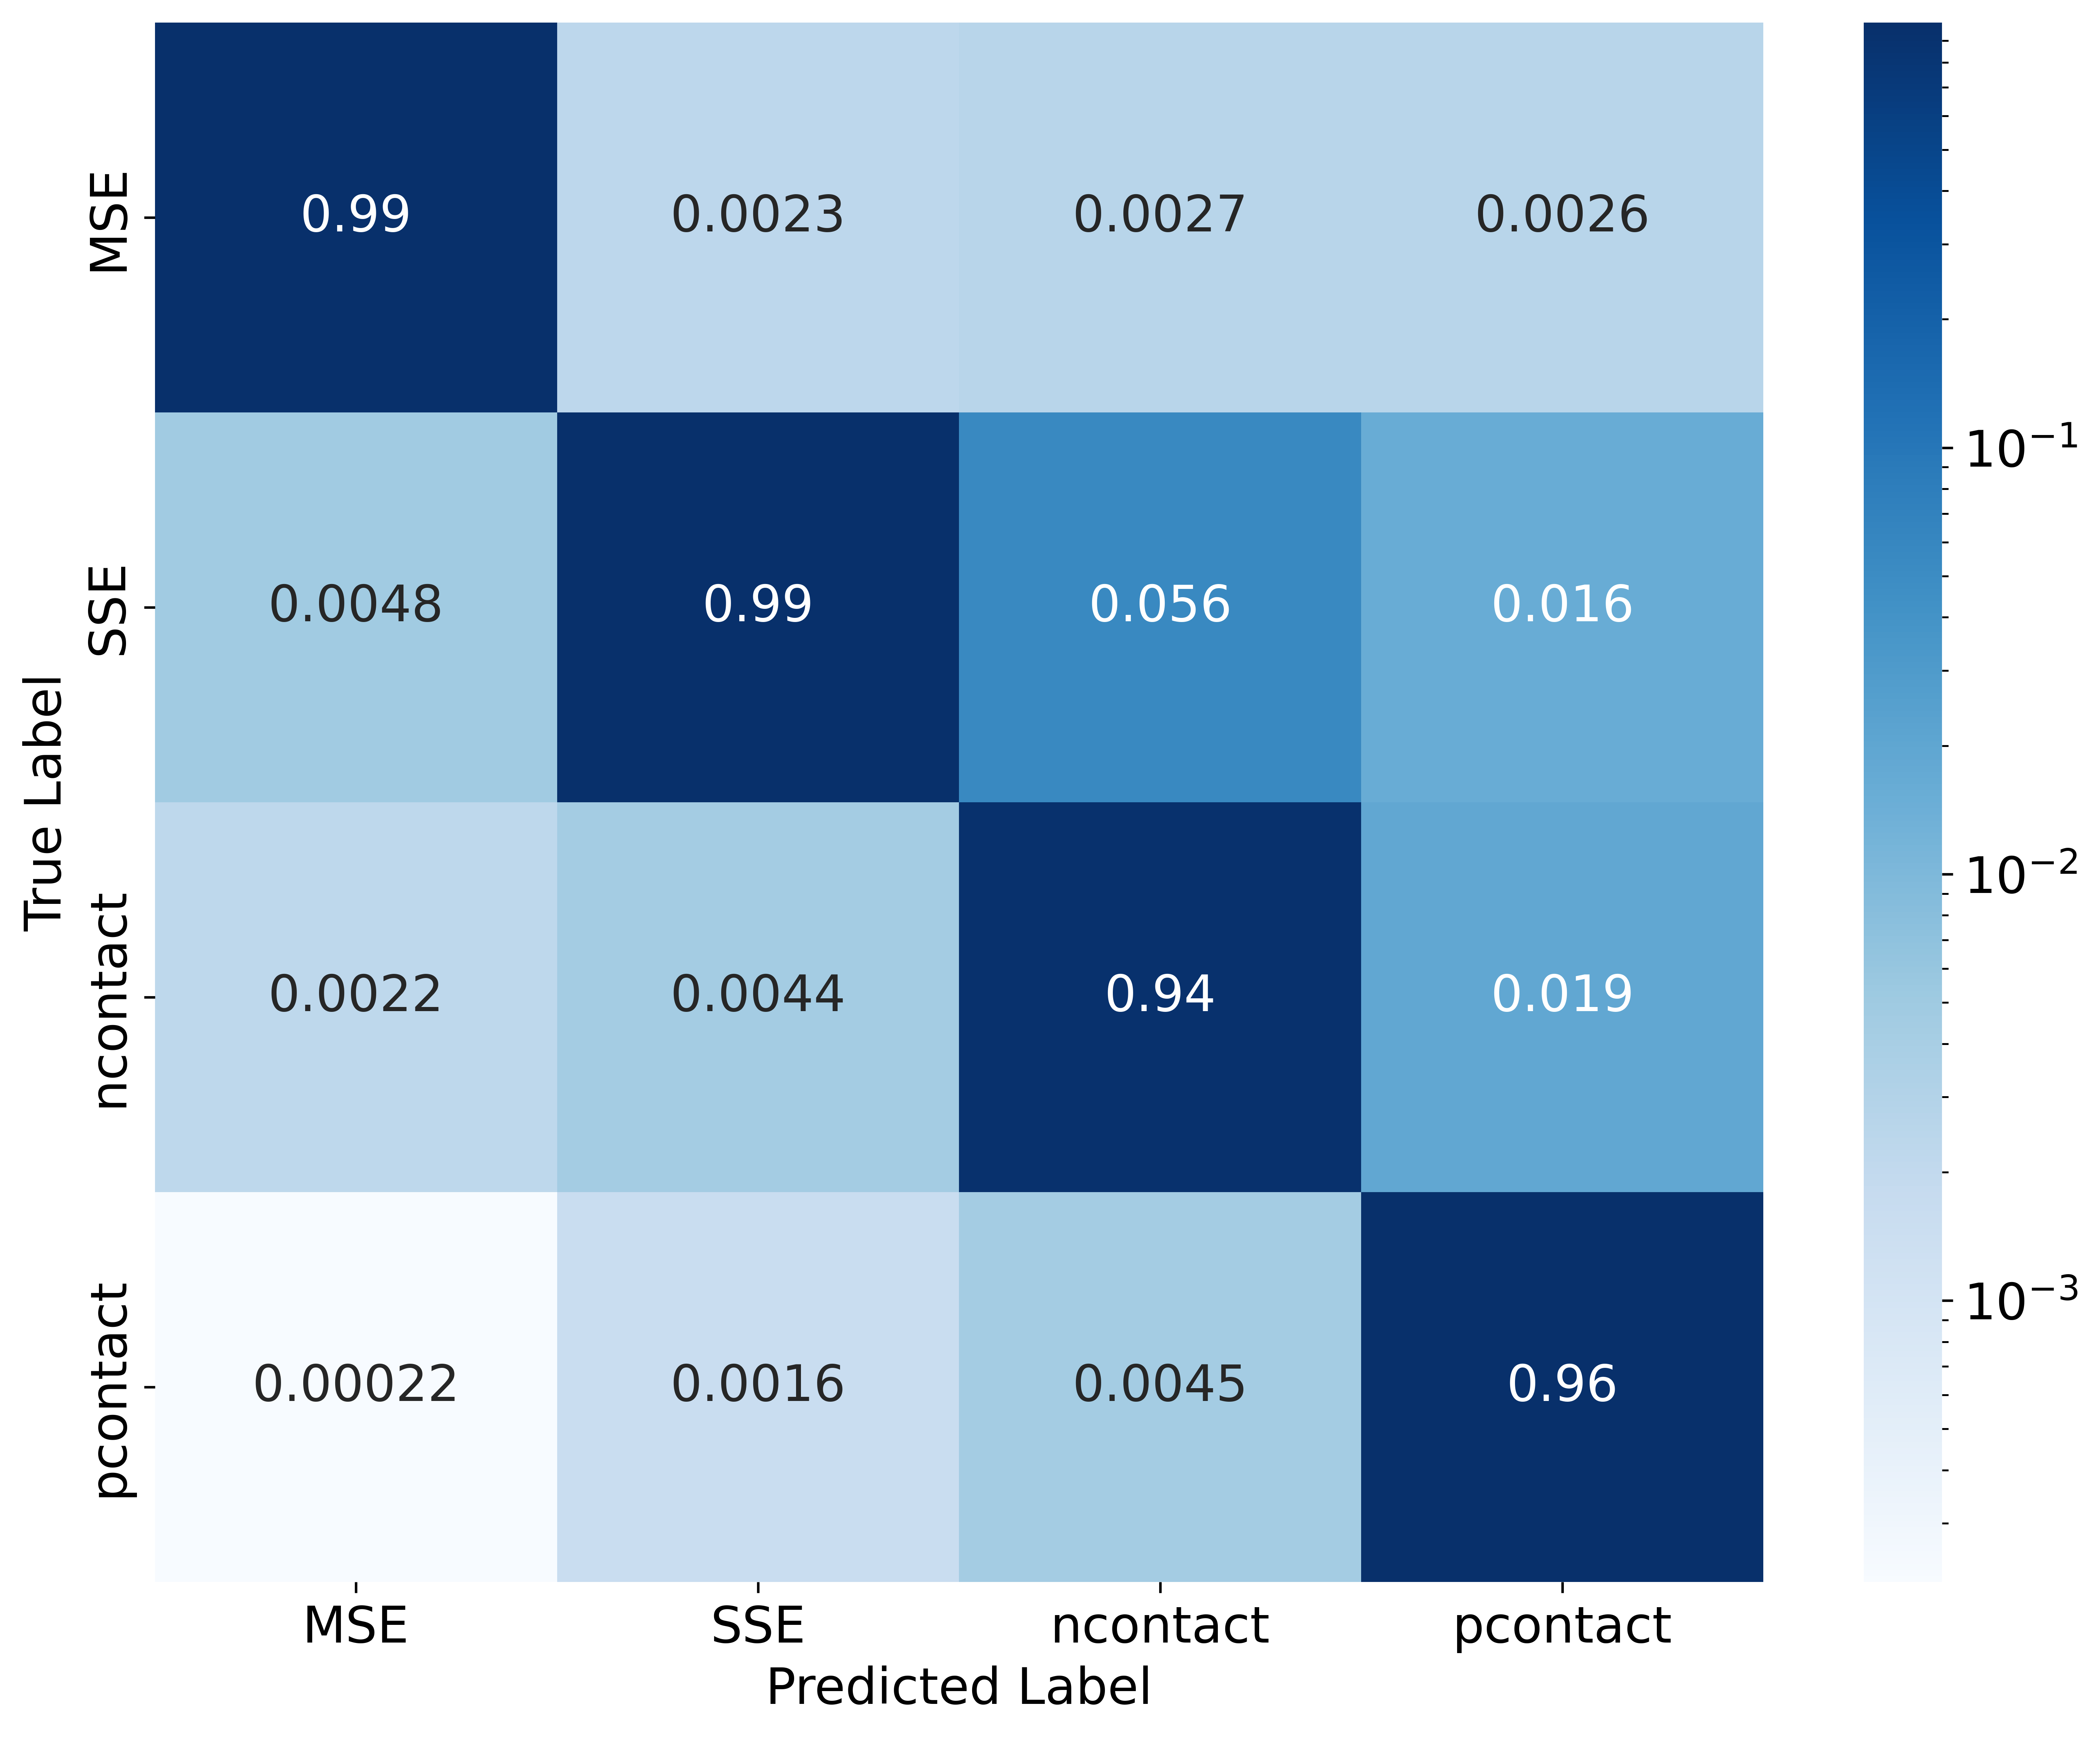
\includegraphics[width=0.75\linewidth]{figures/05_PSD/Results_confusionmatrix_icpc_v1.png}
    \caption{Confusion matrix of model one, with precision scores shown on the diagonal. The model was trained on 12.5 million $^{228}$Th calibration waveforms. Multi-site and single-site events are classified with high precision ($>99\%$), while both surface event types show some misclassification but still achieve precision scores above 90\%.} 
\label{fig:Confusionmatrix_icpc_v1}
\end{figure}

\begin{table}
\centering
\caption{Classification scores for the first Transformer model. Precision is the fraction of correct positive predictions, while sensitivity refers to the fraction of true positives correctly identified. The F1-score combines both.}
\begin{tabular}{||c | c | c | c | c||} 
 \hline
 \textbf{Class} & \textbf{Precision} & \textbf{Sensitivity} & \textbf{F1-score} & \textbf{Support} [$\times 10^6$] \\ 
 \hline
 SSE & 0.992 & 0.925 & 0.957 & 1.03 \\
 \hline
 MSE & 0.993 & 0.996 & 0.994 & 1.47 \\
  \hline
 n$^+$ & 0.937 & 0.992 & 0.964 & 1.15 \\
 \hline
 p$^+$ & 0.963 & 0.937 & 0.950 & 0.12 \\
 \hline
 Weighted avg	&  0.975 & 0.974 & 0.974 & 3.76  \\ 
 \hline
\end{tabular}
\label{tab:Scores_icpc_v1}
\end{table}


\subsubsection{Second Transformer model} 

For the second model, the training data was extended. In addition to the four primary $^{228}$Th calibration peaks, we included seven additional energy peaks from a dedicated $^{56}$Co calibration run, all of which are DEPs: 1012.8~keV, 1576.5~keV, 1987.6~keV, 2180.0~keV, 2231.5~keV, 2251.1~keV, and 2429.2~keV. 

Using additional energy regions should improve the model's flexibility.
Furthermore, the two surface event classes (n$^+$ and p$^+$) were merged into a single surface label. Apart from these changes, the second model is architecturally identical to the first.

This resulted in a total of 11 distinct energy regions, used to extract 14 million waveforms for training. The resulting model demonstrates classification precision across all event types ($98\%$), shown in the confusion matrix in figure~\ref{fig:Confusionmatrix_icpc_v2}, and the summary table~\ref{tab:Scores_icpc_v2}. Furthermore, the model achieves exceptionally high sensitivity across all classes, all with F1-scores exceeding 98\%. While such uniformly high scores indicated excellent classification performance, it's important to check that this isn't due to overfitting. 

\begin{figure}[t]
    \centering
    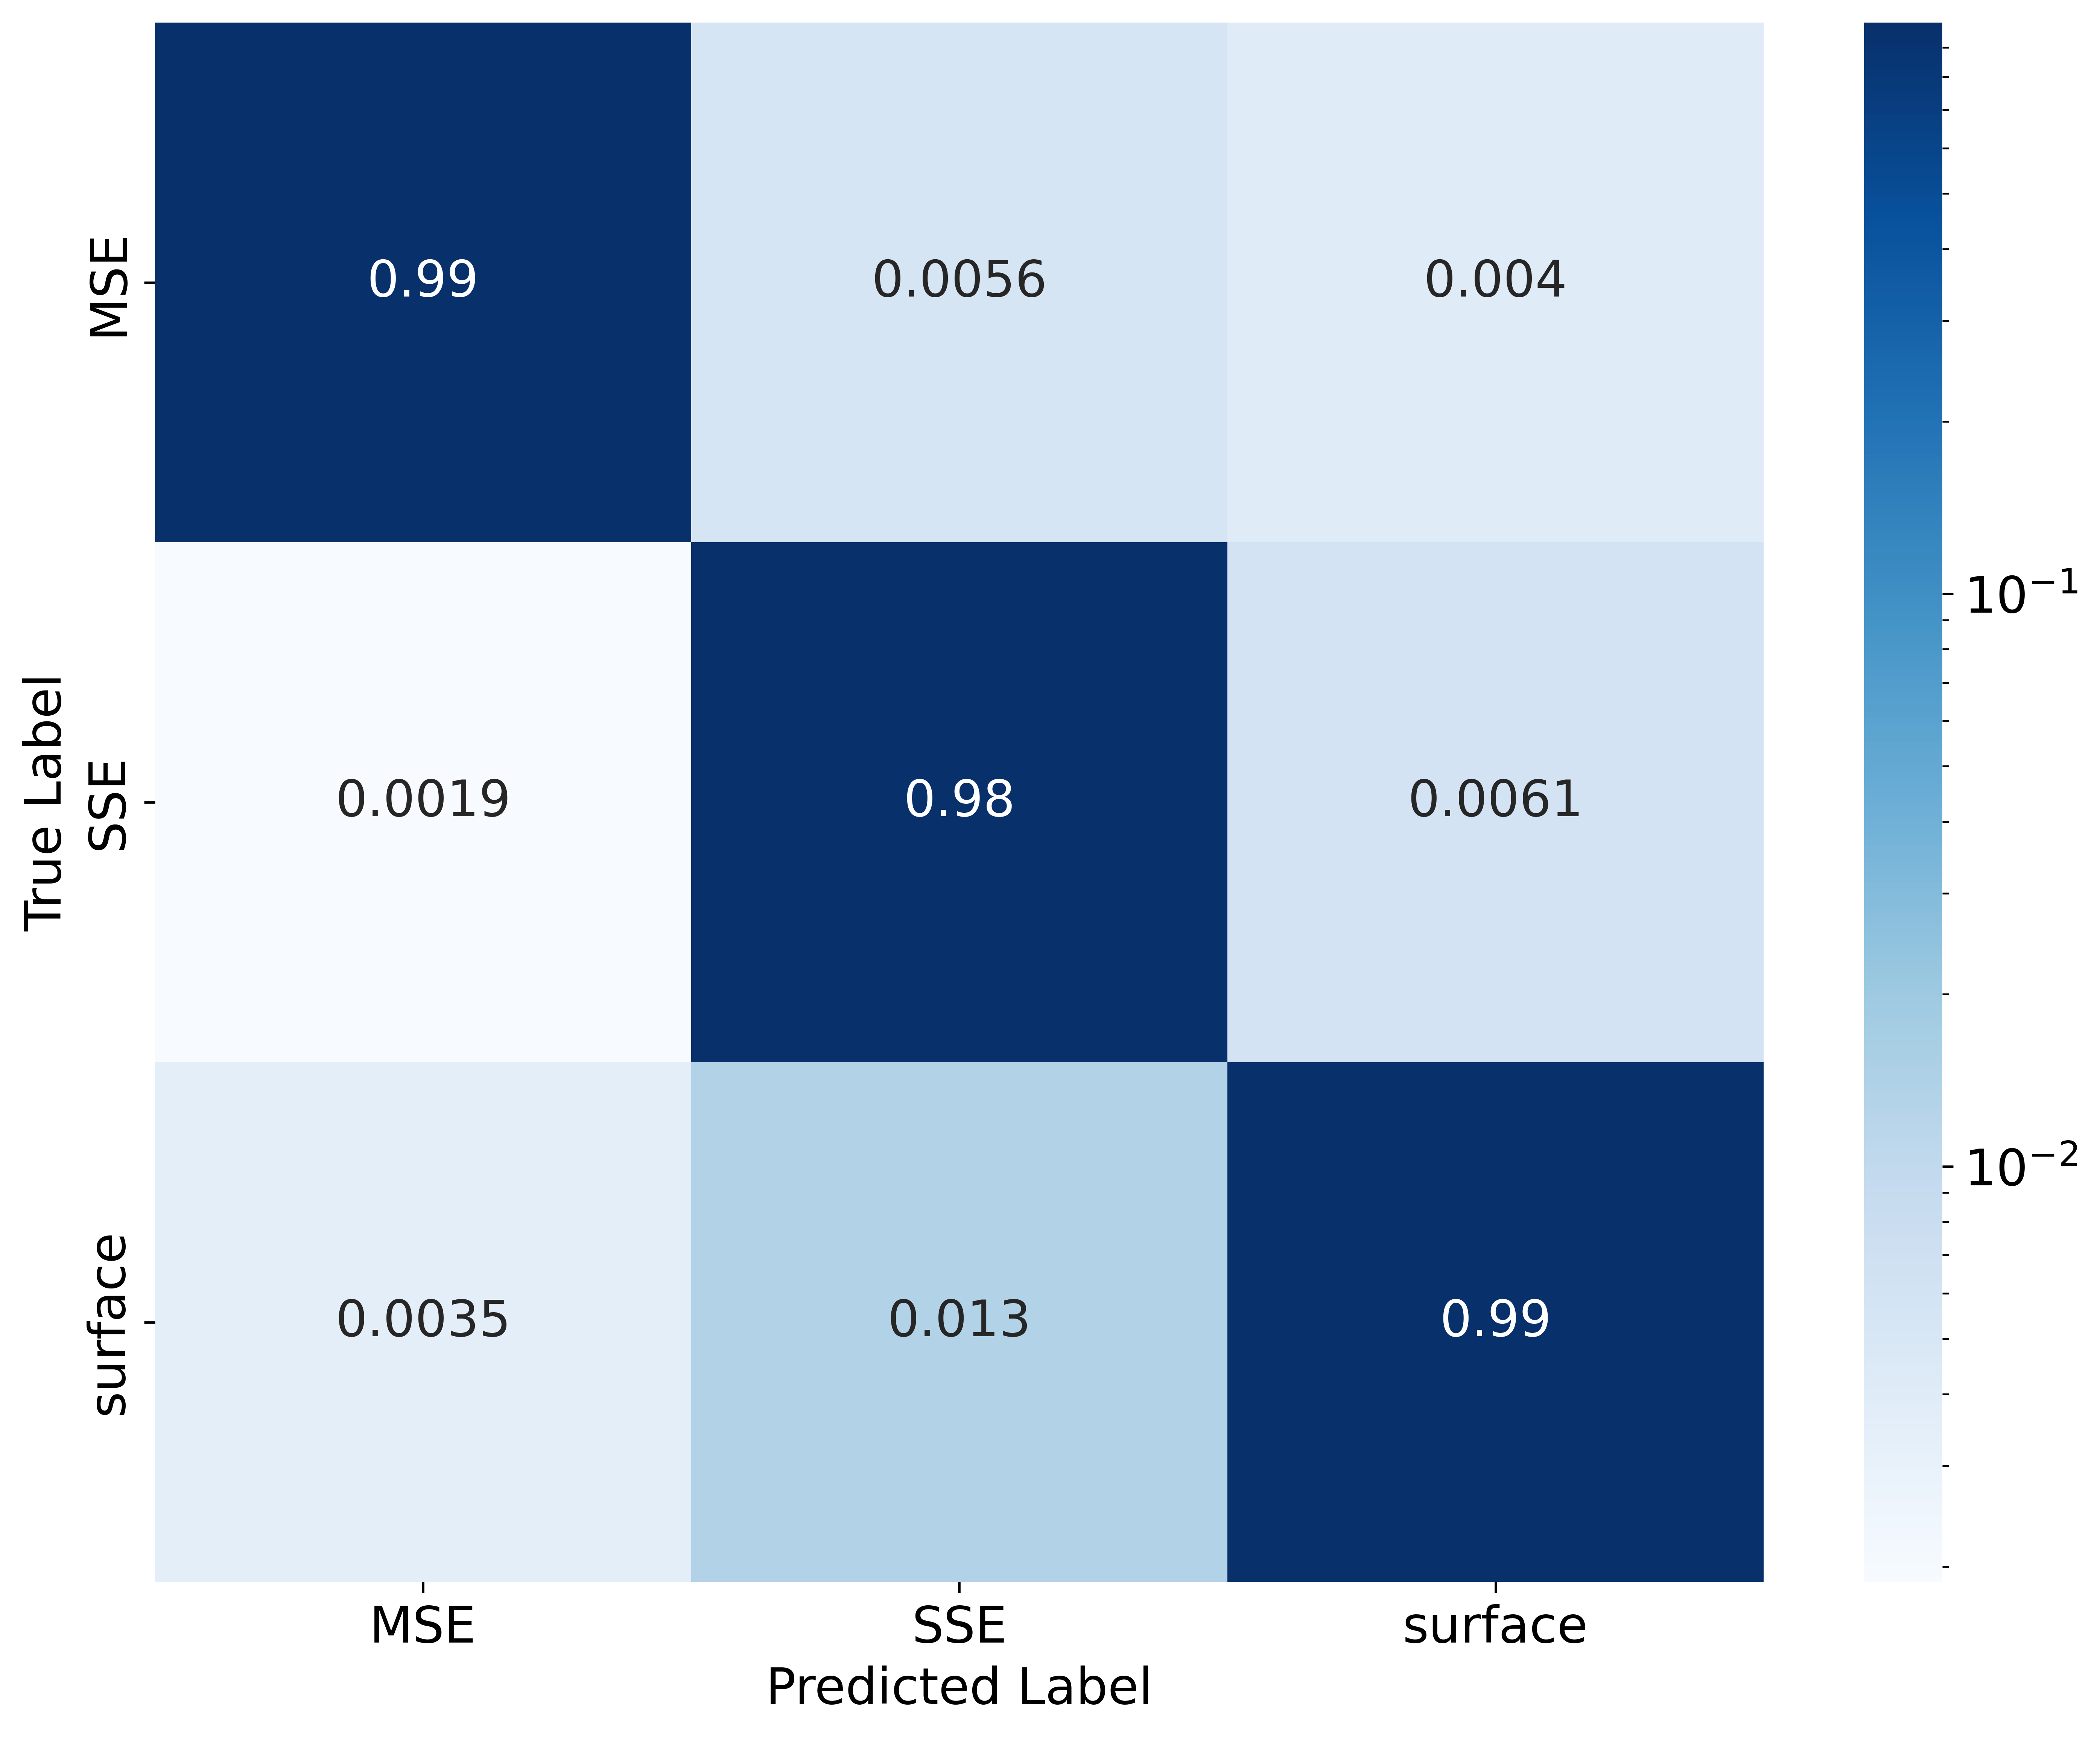
\includegraphics[width=0.75\linewidth]{figures/05_PSD/Results_confusionmatrix_icpc_v2.png}
    \caption{Confusion matrix of model two, where we trained on 14.0 million events. This testing includes 3.3 million events. All event categories are classified with high precision, each exceeding 98\%.} 
\label{fig:Confusionmatrix_icpc_v2}
\end{figure}


\begin{table}
\centering
\caption{Classification scores for the second Transformer model: Precision and sensitivity exceed 98\% for all classes.}
\begin{tabular}{||c | c | c | c | c||} 
 \hline
 \textbf{Class} & \textbf{Precision} & \textbf{Sensitivity} & \textbf{F1-score} & \textbf{Support} [$\times 10^6$] \\ 
 \hline
 SSE & 0.981 & 0.989 & 0.985 & 0.61 \\
 \hline
 MSE & 0.995 & 0.993 & 0.994 & 0.40 \\
  \hline
 surface & 0.990 & 0.986 & 0.988 & 0.55 \\
 \hline
 Weighted avg & 0.989 & 0.989 & 0.989 & 1.56 \\ 
 \hline
\end{tabular}
\label{tab:Scores_icpc_v2}
\end{table}



\subsubsection{Third Transformer model}

A third model was also prepared using a new dataset based on $^{228}$Th and $^{56}$Co calibration data. While it covered the same energy regions as the second model, we wanted to maintain the balance between the two different calibrations. Therefore, we selected only a single $^{228}$Th calibration period (period 3). In addition, the surface-event labels were separated again into distinct p$^+$ and n$^+$ categories. 
However, this model performed poorly: it failed to generalize beyond the training data and exhibited inconsistent classification across detectors. Due to these issues, the model was deemed unsuitable for further evaluation and was excluded from the analysis. The exact cause of the poor performance remains unclear, but it may be related to the label noise in the $^{56}$Co dataset. 


\subsubsection{Network comparison and performance on \texorpdfstring{$2 \nu \beta \beta$ decay events}{}}

The classification scores of the three Transformer models were evaluated on a test dataset consisting of calibration events at well-defined $\gamma$-ray energy peaks. For the PSD cut to be applicable in LEGEND-200, the models must generalize beyond these narrow energy regions, in particular to the vicinity of $Q_{\beta \beta} = 2039$~keV. Reliable single-site classification at lower energies is important, as it enables validation of PSD efficiency using the continuous $2 \nu \beta \beta$ decay spectrum present in physics data. In particular, the energy range between 1000 and 1300~keV, used in this analysis to extract the PSD efficiency at $Q_{\beta \beta}$, is a key validation region. Figure~\ref{fig:SSE_cuts_2vbb} shows that, for $E < 1$~MeV, only model 1 maintains a stable SSE efficiency across the spectrum, whereas the other models exhibit inconsistent behavior.  



\begin{figure}[t]
    \centering
    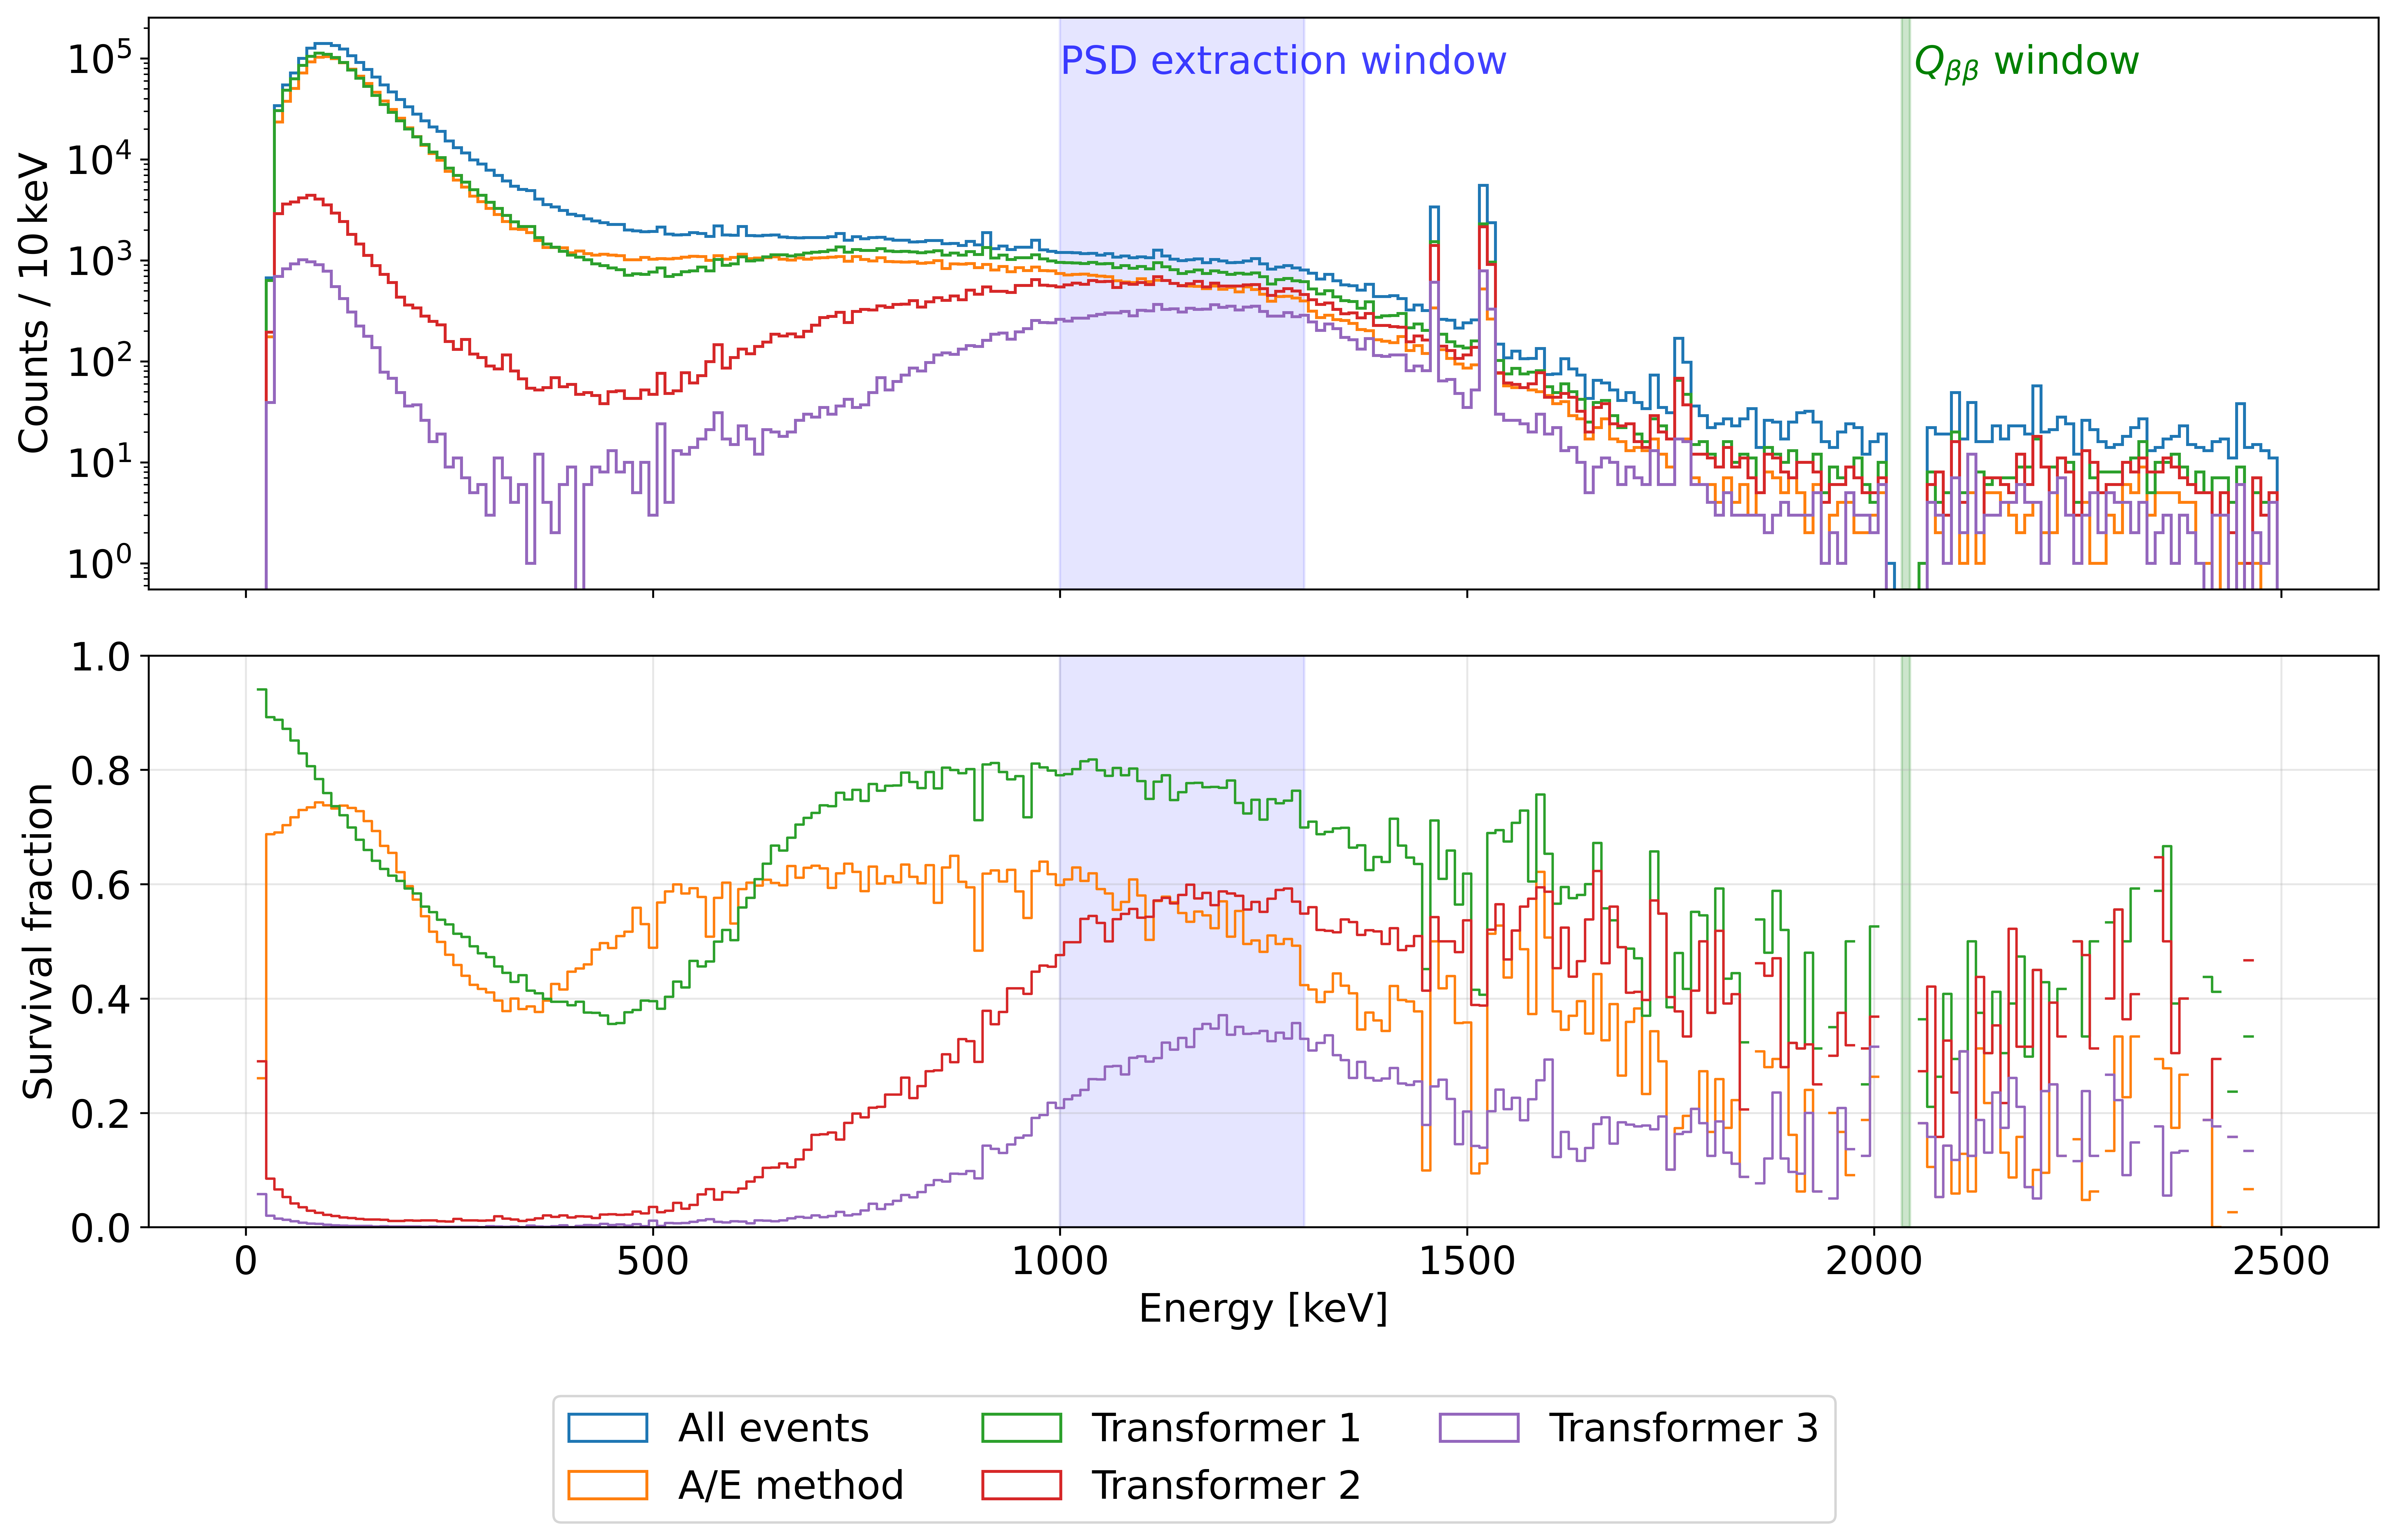
\includegraphics[width=\linewidth]{figures/05_PSD/SSE_cuts_2vbb.png}
    \caption{Energy spectra of the $2 \nu \beta \beta$ decay population, with different PSD cuts, applied (top), and the corresponding survival fractions (bottom). The spectra include all physics runs listed in section~\ref{sec:04_LEGEND_data}, corresponding to a total exposure of $40.3\, \mathrm{kg} \cdot \mathrm{yr}$. We see that Transformer models 2 and 3 generalize very poorly for the low-energy part of the spectrum, while the A/E cut generally works better at very low energies. }
\label{fig:SSE_cuts_2vbb}
\end{figure}



\subsection{Pulse shape discrimination efficiency at \texorpdfstring{$Q_{\beta \beta}$}{}}
To evaluate the effect of PSD efficiencies on the expected $0 \nu \beta \beta$ decay half-life, the PSD efficiency at $Q_{\beta \beta}$, denoted as $\epsilon_{\mathrm{PSD}}$, must be determined. We adopt a similar procedure as developed by the LEGEND-200 collaboration, described in~\cite{lnote_24013}. 
In this analysis, only Mirion ICPC detectors are considered, which allows for consistent PSD cut definitions throughout the full analysis. Furthermore, the LEGEND-200 collaboration has decided to focus on ICPC detectors. Since we have no pure SSE populations at $Q_{\beta \beta}$ to estimate the efficiencies, we assume a linear energy dependence and extrapolate the efficiency at $Q_{\beta \beta}$. 

We therefore calculate the PSD efficiency as:

\begin{equation}
\label{eq:psd_eff_qbb}
    \epsilon_{\mathrm{PSD}} = \tilde{\epsilon}_{\mathrm{PSD}} + \langle \delta_{\mathrm{run}} \rangle + \epsilon_{2 \nu \beta \beta} \,,
\end{equation}

\noindent where $\tilde{\epsilon}_{\mathrm{PSD}}$ denotes the uncorrected PSD efficiency at $Q_{\beta \beta}$. The correction term $\langle \delta_{\mathrm{run}} \rangle$ accounts for time-dependent variations in the PSD performance during data taking, and $\epsilon_{2 \nu \beta \beta}$, compensates for differences in the single-site event population between $2 \nu \beta \beta$ decays and the double escape peak calibration data. 
The energy dependence of SSE detection efficiency using the A/E parameters arises from three main physical effects \cite{comellato_topologies_2023}: 

\begin{enumerate}
    \item Bremsstrahlung becomes more probable at higher energies, leading to the emission of secondary photons. This can spatially separate the energy deposition and reduce the A/E value, causing SSEs to be misclassified as MSE, thereby lowering the detection efficiency at $Q_{\beta \beta}$ compared to the $^{208}$Tl DEP~\cite{comellato_charge_2021}.
    \item Charge cloud self-repulsion increases with energy due to a higher number of induced charges. This results in longer drift times and broader waveforms, which in turn reduce the signal amplitude and the A/E value. As a result, the detection efficiency at $Q_{\beta \beta}$ is further reduced~\cite{Radford_2012}. 
    \item Electronic noise becomes less relevant at higher energies, which tends to increase the detection efficiency. However, this effect is generally outweighed by the first two.
\end{enumerate}

Together, these effects imply that the PSD efficiency decreases at higher energies. In this work, we estimate the PSD efficiency at three different energy regions. The method for extracting the efficiency in each region is presented in the following subsections:

\begin{itemize}
	\item In the 1000-1300 keV interval, using the $2 \nu \beta \beta$ decay background (PSD extraction window)
	\item At the 1592.5 keV DEP from $^{208}$Tl
	\item At the 2231.5 keV DEP from $^{56}$Co.
\end{itemize}


\subsubsection{PSD efficiency for \texorpdfstring{$2 \nu \beta \beta$}{} decay events}

To estimate the PSD efficiency for $2 \nu \beta \beta$ decay events, the Transformer models were tested on all periods listed in table~\ref{tab:periods_runs} for a total exposure of $40.3\, \mathrm{kg} \cdot \mathrm{yr}$. The PSD efficiency can be evaluated at different energy regions within the spectrum. For this analysis, we use the 1000-1300 keV window because this region offers high statistics and is relatively free from prominent gamma lines.
An alternative energy range between 1525 and 1750 keV could be used if contributions from gamma lines are subtracted. However, this region suffers from significantly lower event statistics. Therefore, we rely exclusively on the lower-energy window for the PSD efficiency extraction. It is estimated as follows:

\begin{equation}
\label{eq:eff_2vbb}
    \epsilon_{2 \nu \beta \beta} = \frac{\frac{T_p}{T_p + T_f} - \lambda_B \lambda_{Bp}}{1 - \lambda_B} \,.
\end{equation}

\noindent Here, $T_p$ and $T_f$ denote the number of events that pass or fail the PSD cuts, respectively. 
The parameter $\lambda_B$ represents the fraction of events in the window that originate from the background, and $\lambda_{Bp}$ is the fraction of those background events that pass the cuts. 

The value of $\lambda_{B}$ is derived from the expected number of $2 \nu \beta \beta$ decays based on exposure, detection efficiency, and the known half-life. A detailed background analysis for LEGEND-200 by Calgaro et al. determined $\lambda_B = (8.7 \pm 1.7) \%$, which we adopt in this analysis~\cite{lnote_24007}. 

Assuming the background events are equally likely to pass or fail the PSD cut, we set $\lambda_{Bp} = (50 \pm \frac{1}{\sqrt{12}})~\% $, corresponding to a uniform distribution. The uncertainty on $T_p$ and $T_f$ is assumed to follow Poisson statistics.
The uncertainty on $\epsilon_{2 \nu \beta \beta}$ is given by

\begin{align}
\sigma_{\epsilon_{2 \nu \beta \beta}} = \Bigg[ &
\left( \frac{\partial \epsilon}{\partial T_p} \cdot \sigma_{T_p} \right)^2
+ \left( \frac{\partial \epsilon}{\partial T_f} \cdot \sigma_{T_f} \right)^2 \notag \\
& + \left( \frac{\partial \epsilon}{\partial \lambda_B} \cdot \sigma_{\lambda_B} \right)^2
+ \left( \frac{\partial \epsilon}{\partial \lambda_{Bp}} \cdot \sigma_{\lambda_{Bp}} \right)^2
\Bigg]^{1/2} \notag \\
= \Bigg[ &
\left( \frac{\frac{T_f}{(T_p + T_f)^2}}{1 - \lambda_B} \cdot \sigma_{T_p} \right)^2 
+ \left( \frac{\frac{-T_p}{(T_p + T_f)^2}}{1 - \lambda_B} \cdot \sigma_{T_f} \right)^2 \notag \\
& + \left( \frac{\frac{T_p}{T_p + T_f} - \lambda_{Bp}}{(1 - \lambda_B)^2} \cdot \sigma_{\lambda_B} \right)^2
+ \left( \frac{-\lambda_B}{1 - \lambda_B} \cdot \sigma_{\lambda_{Bp}} \right)^2 \Bigg]^{1/2}
\label{eff_2vbb_err} \,.
\end{align}


\subsubsection{PSD efficiency at double escape peaks}

The PSD efficiency at the double escape peaks is determined by fitting the peaks separately for events that pass and events that fail the PSD cut. Example fits are shown in figure~\ref{fig:peakfit_example_Tl} and figure~\ref{fig:peakfit_example_Co} for the $^{208}$Tl and $^{56}$Co DEPs, respectively.  
The full fit function is given by:

\begin{equation}
\label{eq:fit_function_gauss_lin_step}
    f(x, A, \mu, \sigma, a, b, d) = A \cdot e^{\frac{-(x - \mu)^2}{2 \sigma^2}} + \frac{d}{2} \cdot \mathrm{erfc} \left[ \frac{x - \mu}{\sqrt{2} \cdot \sigma} \right] + a \cdot x + b \,,
\end{equation}

\noindent where $\mathrm{erf}(x)$ is the complementary Gaussian error function, given by equation~\refeq{eq:erfc}. The parameters of the fit are the amplitude $A$, mean $\mu$, and standard deviation $\sigma$ of the Gaussian, the slope $a$ and intercept $b$ of the background, and the size of the step function $d$.   

\begin{equation}
\label{eq:erfc}
    \mathrm{erfc}(x) = 1 - \mathrm{erf}(x) = 1 - \frac{2}{\sqrt{\pi}} \int_0^z e^{-t^2} \mathrm{d}t \,.
\end{equation}


\begin{figure}[t]
    \centering
    \includegraphics[width=\linewidth]{figures/05_PSD/Peakfit_Tl208_V00048A.png}
    \caption{Peak fitting results in the $^{208}$Tl DEP region. Each subfigure shows three histograms: all events (blue), events passing the PSD cut (green), and events failing the cut (red). The corresponding fits are shown as line plots. The two lower panels display the normalized residuals for the fit to the passing (middle) and failing (bottom) event populations. The residuals confirm the quality and stability of the fits.} 
\label{fig:peakfit_example_Tl}
\end{figure}


\begin{figure}[t]
    \centering
    \includegraphics[width=\linewidth]{figures/05_PSD/Peakfit_Co56_V00048A.png}
    \caption{Peak fitting results in the $^{56}$Co DEP region. Each subfigure shows three histograms: all events (blue), events passing the PSD cut (green), and events failing the cut (red). The corresponding fits are shown as line plots. The two lower panels display the normalized residuals for the fit to the passing (middle) and failing (bottom) event populations. The residuals confirm the quality and stability of the fits. } 
\label{fig:peakfit_example_Co}
\end{figure}


The linear background is justified since we fit a narrow window of $\pm 20$~keV around the peak. The step function is to account for low- and high-energy tails. 
The PSD efficiency and its uncertainty are subsequently computed from the background-subtracted peak amplitude determined in the fit:

\begin{align}
\label{eq:eff_DEP}
    \epsilon_{\mathrm{DEP}} & = \frac{A_p}{A_p + A_f} \\
    \sigma_{\epsilon_{\mathrm{DEP}}} & = \epsilon_{\mathrm{DEP}} \cdot (1 - \epsilon_{\mathrm{DEP}}) \cdot \sqrt{\left(\frac{\sigma_p}{A_p} \right)^2 + \left( \frac{\sigma_f}{A_f} \right)^2} \,,
\label{eq:eff_DEP_err}
\end{align}

\noindent where $A_p$ and $A_f$ are the amplitudes of the Gaussian fits for events that pass and fail the cut, respectively, $\sigma_p$ and $\sigma_f$ are their corresponding uncertainties. The upper plots in figures~\ref{fig:peakfit_example_Tl} and~\ref{fig:peakfit_example_Co} show these fits. 
The A/E parameter is calibrated such that approximately 90\% of events in the DEP region are classified as single-site. Consequently, only a small number of events are expected to fail the cut, which can lead to large uncertainties in $A_f$ due to low statistics.

We determine the PSD efficiency individually for each detector. To obtain an overall value, we initially computed a weighted average of the individual efficiencies. To account for potential inconsistencies between detectors, we applied Particle Data Group-style uncertainty scaling: if the spread of the efficiencies is larger than expected from their statistical uncertainties, the combined uncertainty is scaled by a factor $S = \sqrt{\chi^2/\mathrm{dof}}$. This avoids underestimating the total uncertainty if there are unaccounted systematic uncertainties between detectors~\cite{navas_review_2024}. In principle, this method is justified since the event sets that pass and fail the cut are disjoint. 

However, a poor goodness-of-fit ($\chi^2 = 9$) indicated that the uncertainty reported by the initial fit underestimates the true dispersion in the measurements. 
This discrepancy likely stems from detector-specific effects that are not captured in the statistical errors alone. To account for variations in readout electronics, differences in supply voltages, or other subtle hardware-related factors, we introduce an additional detector-specific uncertainty term, denoted by $\langle \delta_{\mathrm{det}} \rangle$. 
We model the total variance by augmenting each statistical uncertainty with this extra contribution and fit the data using a least-$\chi^2$ method\footnote{To make the connection to section~\ref{sec:03_optimization}: The least $\chi^2$ is equivalent to the negative log-likelihood if we assume the likelihood to be Gaussian.}:

\begin{equation}
\label{eq:chi2_eff_fit}
\chi^2 \left( \epsilon_i, \sigma_{\epsilon, i} \mid \langle \varepsilon \rangle, \langle \delta_{\mathrm{det}} \rangle \right) = 
\sum_i \left[ \frac{(\epsilon_i - \langle \varepsilon \rangle)^2}{\sigma_{\epsilon,i}^2 + \langle \delta_{\mathrm{det}} \rangle^2} + \log\left( \sigma_{\epsilon,i}^2 + \langle \delta_{\mathrm{det}} \rangle^2 \right) \right] \,,
\end{equation}

\noindent where $\epsilon_i$ is the PSD efficiency measured for detector $i$, $\sigma_{\epsilon, i}$ the corresponding statistical uncertainty, $\langle \varepsilon \rangle$ the global average PSD efficiency, and $\langle \delta_{\mathrm{det}} \rangle$ is the additional uncertainty representing unaccounted detector-to-detector variations. 
The logarithmic term ensures proper normalization of the likelihood. 
The resulting PSD efficiencies for the double escape peaks of $^{208}$Tl and $^{56}$Co are shown in figures~\ref{fig:psd_dep_Tl} and~\ref{fig:psd_dep_Co}, respectively. The additional detector-to-detector variances for both DEPs are shown in table~\ref{tab:fit_variances}.

The global PSD efficiency at the DEP peak is obtained as the inverse-variance weighted mean:

\begin{equation}
\label{eq:chi2_eff_fit_mean}
    \langle \hat{\epsilon} \rangle = \frac{ \sum_i \frac{\epsilon_i}{\left( \sigma_{\epsilon, i}^2 + \langle \delta_{\mathrm{det}} \rangle^2 \right)}}{\sum_i \frac{1}{\left( \sigma_{\epsilon, i}^2 + \langle \delta_{\mathrm{det}} \rangle^2 \right)}} \,.
\end{equation}

\noindent The corresponding $1\,\sigma$ uncertainty on the mean efficiency is given by:


\begin{equation}
\label{eq:chi2_eff_fit_std}
    \sigma_{ \langle \hat{\epsilon} \rangle} = \left( \sum_i \frac{1}{\sigma_{\epsilon, i}^2 + \langle \delta_{\mathrm{det}} \rangle^2} \right)^{-1/2} \,,
\end{equation}

\noindent which incorporates both statistical fluctuations and the additional variance due to detector-to-detector differences. 


\begin{figure}
    \centering
    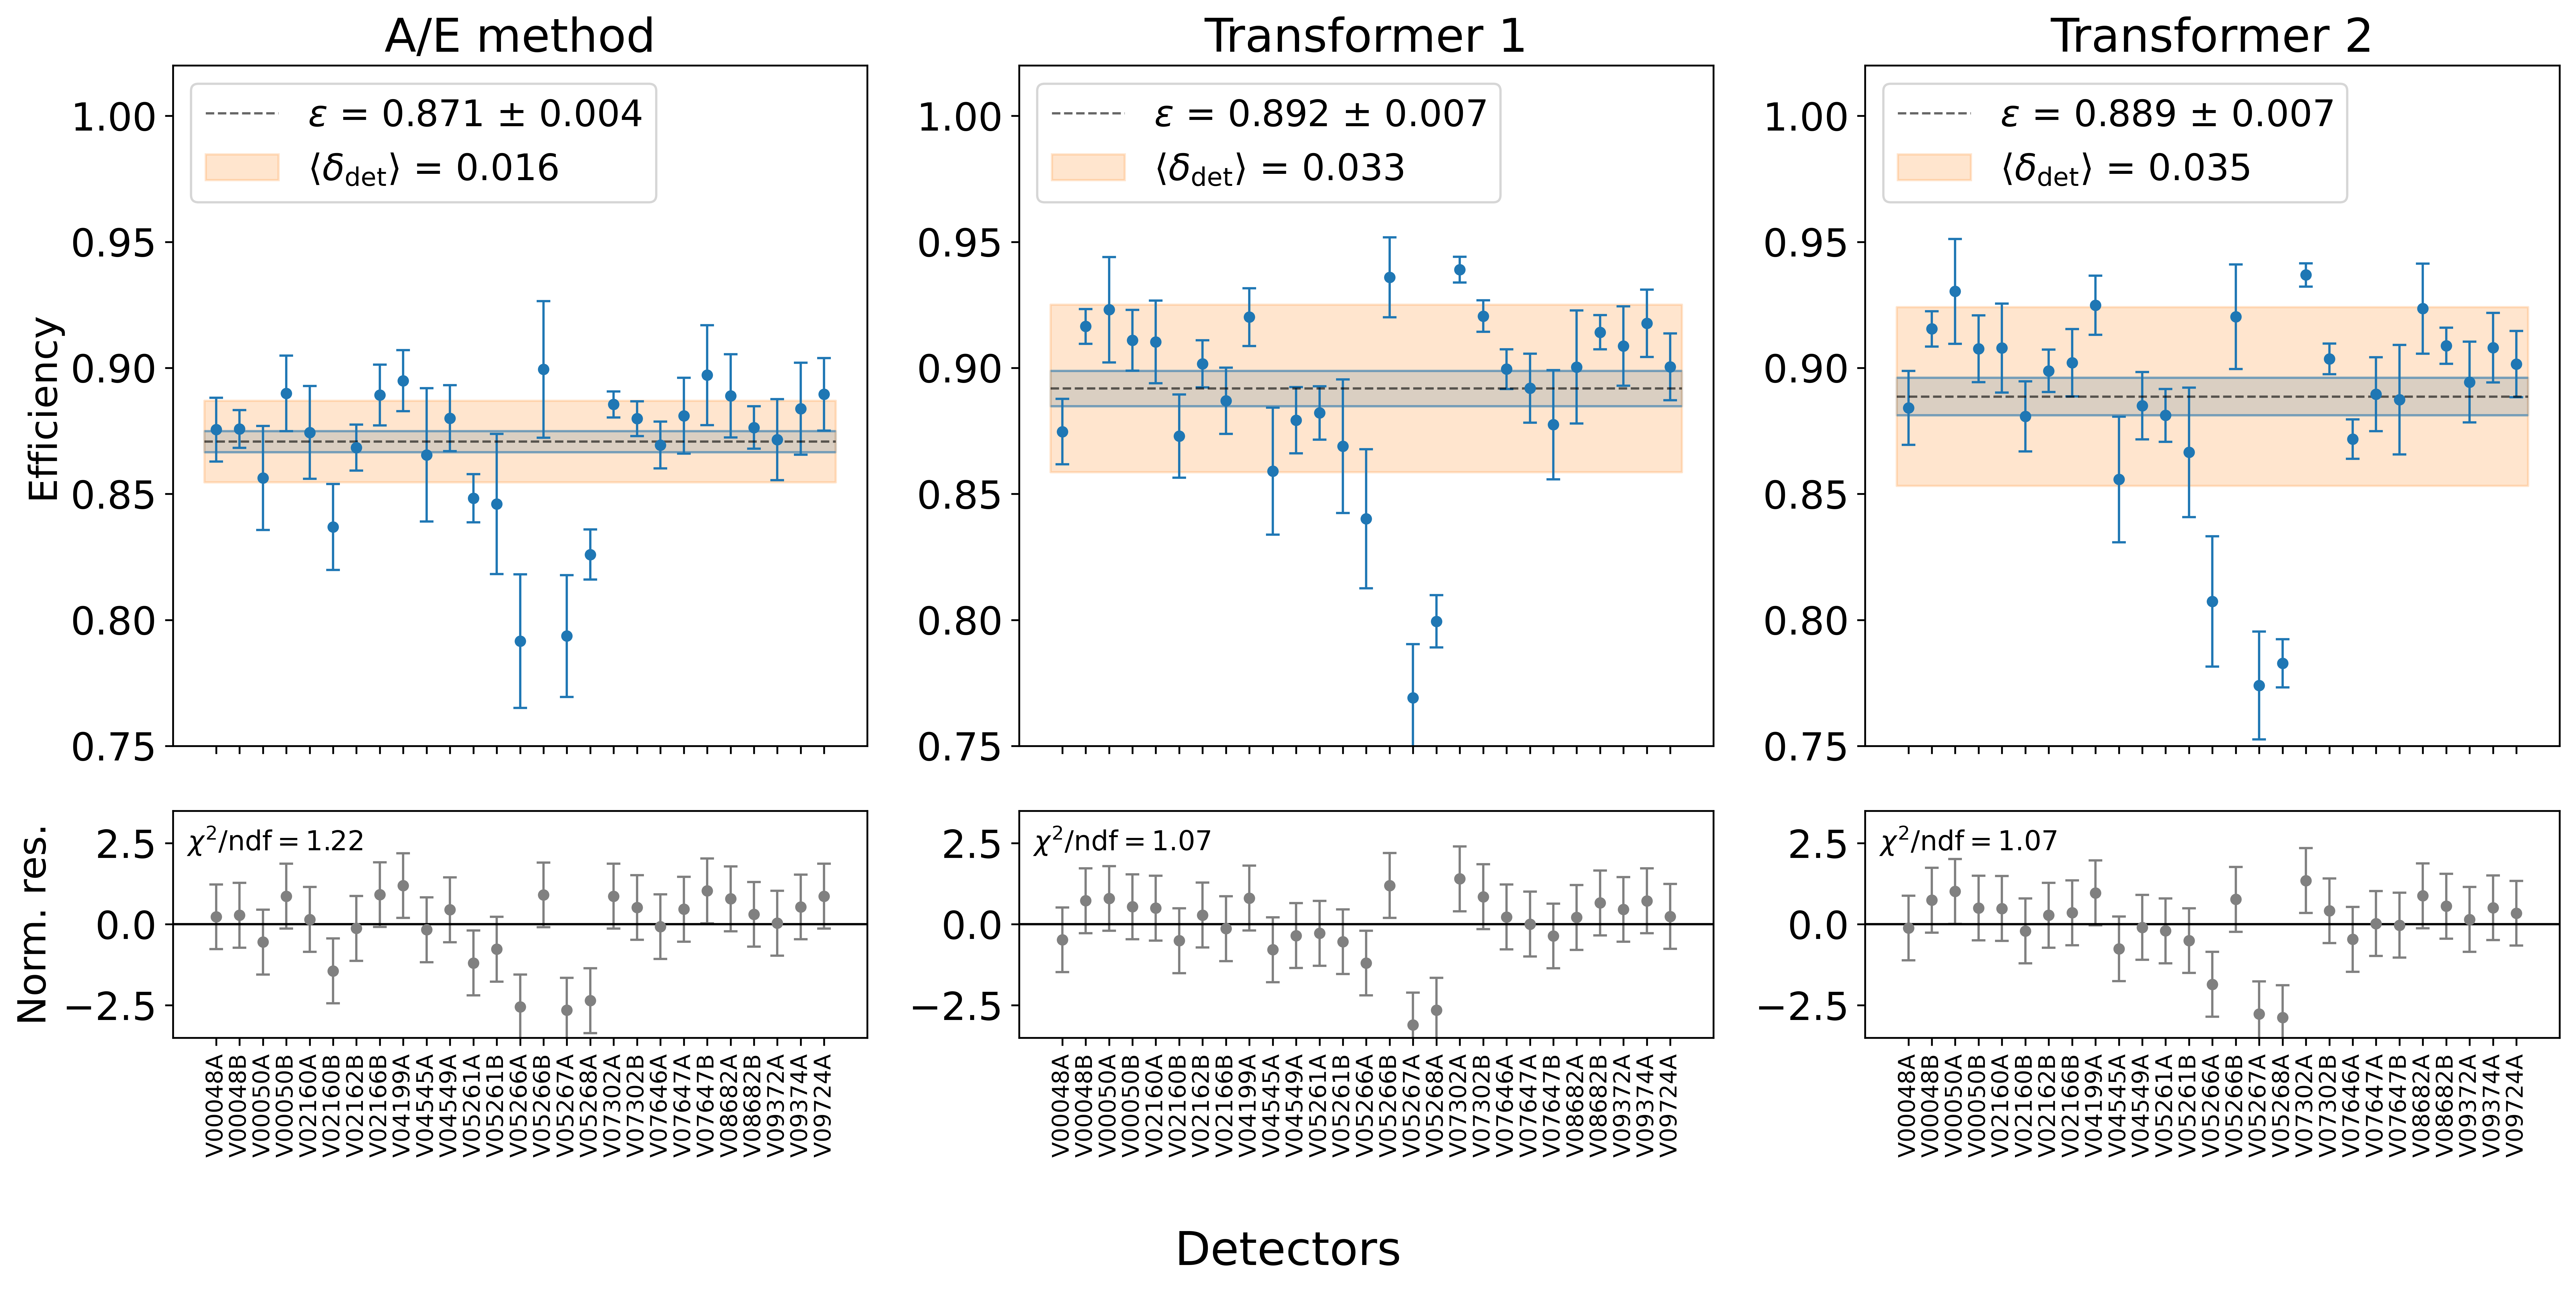
\includegraphics[width=\linewidth]{figures/05_PSD/PSD_eff_DEP_Tl_new.png}
    \caption{PSD efficiencies in the $^{208}$Tl DEP (1592.5~keV) for Mirion detectors used in this analysis. Most detectors exhibit efficiencies (blue band) between 85\% and 90\%, although a few show noticeably lower performance across all PSD methods. The additional detector-to-detector uncertainty is indicated by the orange band. The A/E method shows a small spread ($1.6 \%$), while the Transformer classifications exhibit larger systematic variations ($>3\%$). The lower panel shows the normalized residuals, demonstrating the quality of the fit.} 
\label{fig:psd_dep_Tl}
\end{figure}


\begin{figure}[t]
    \centering
    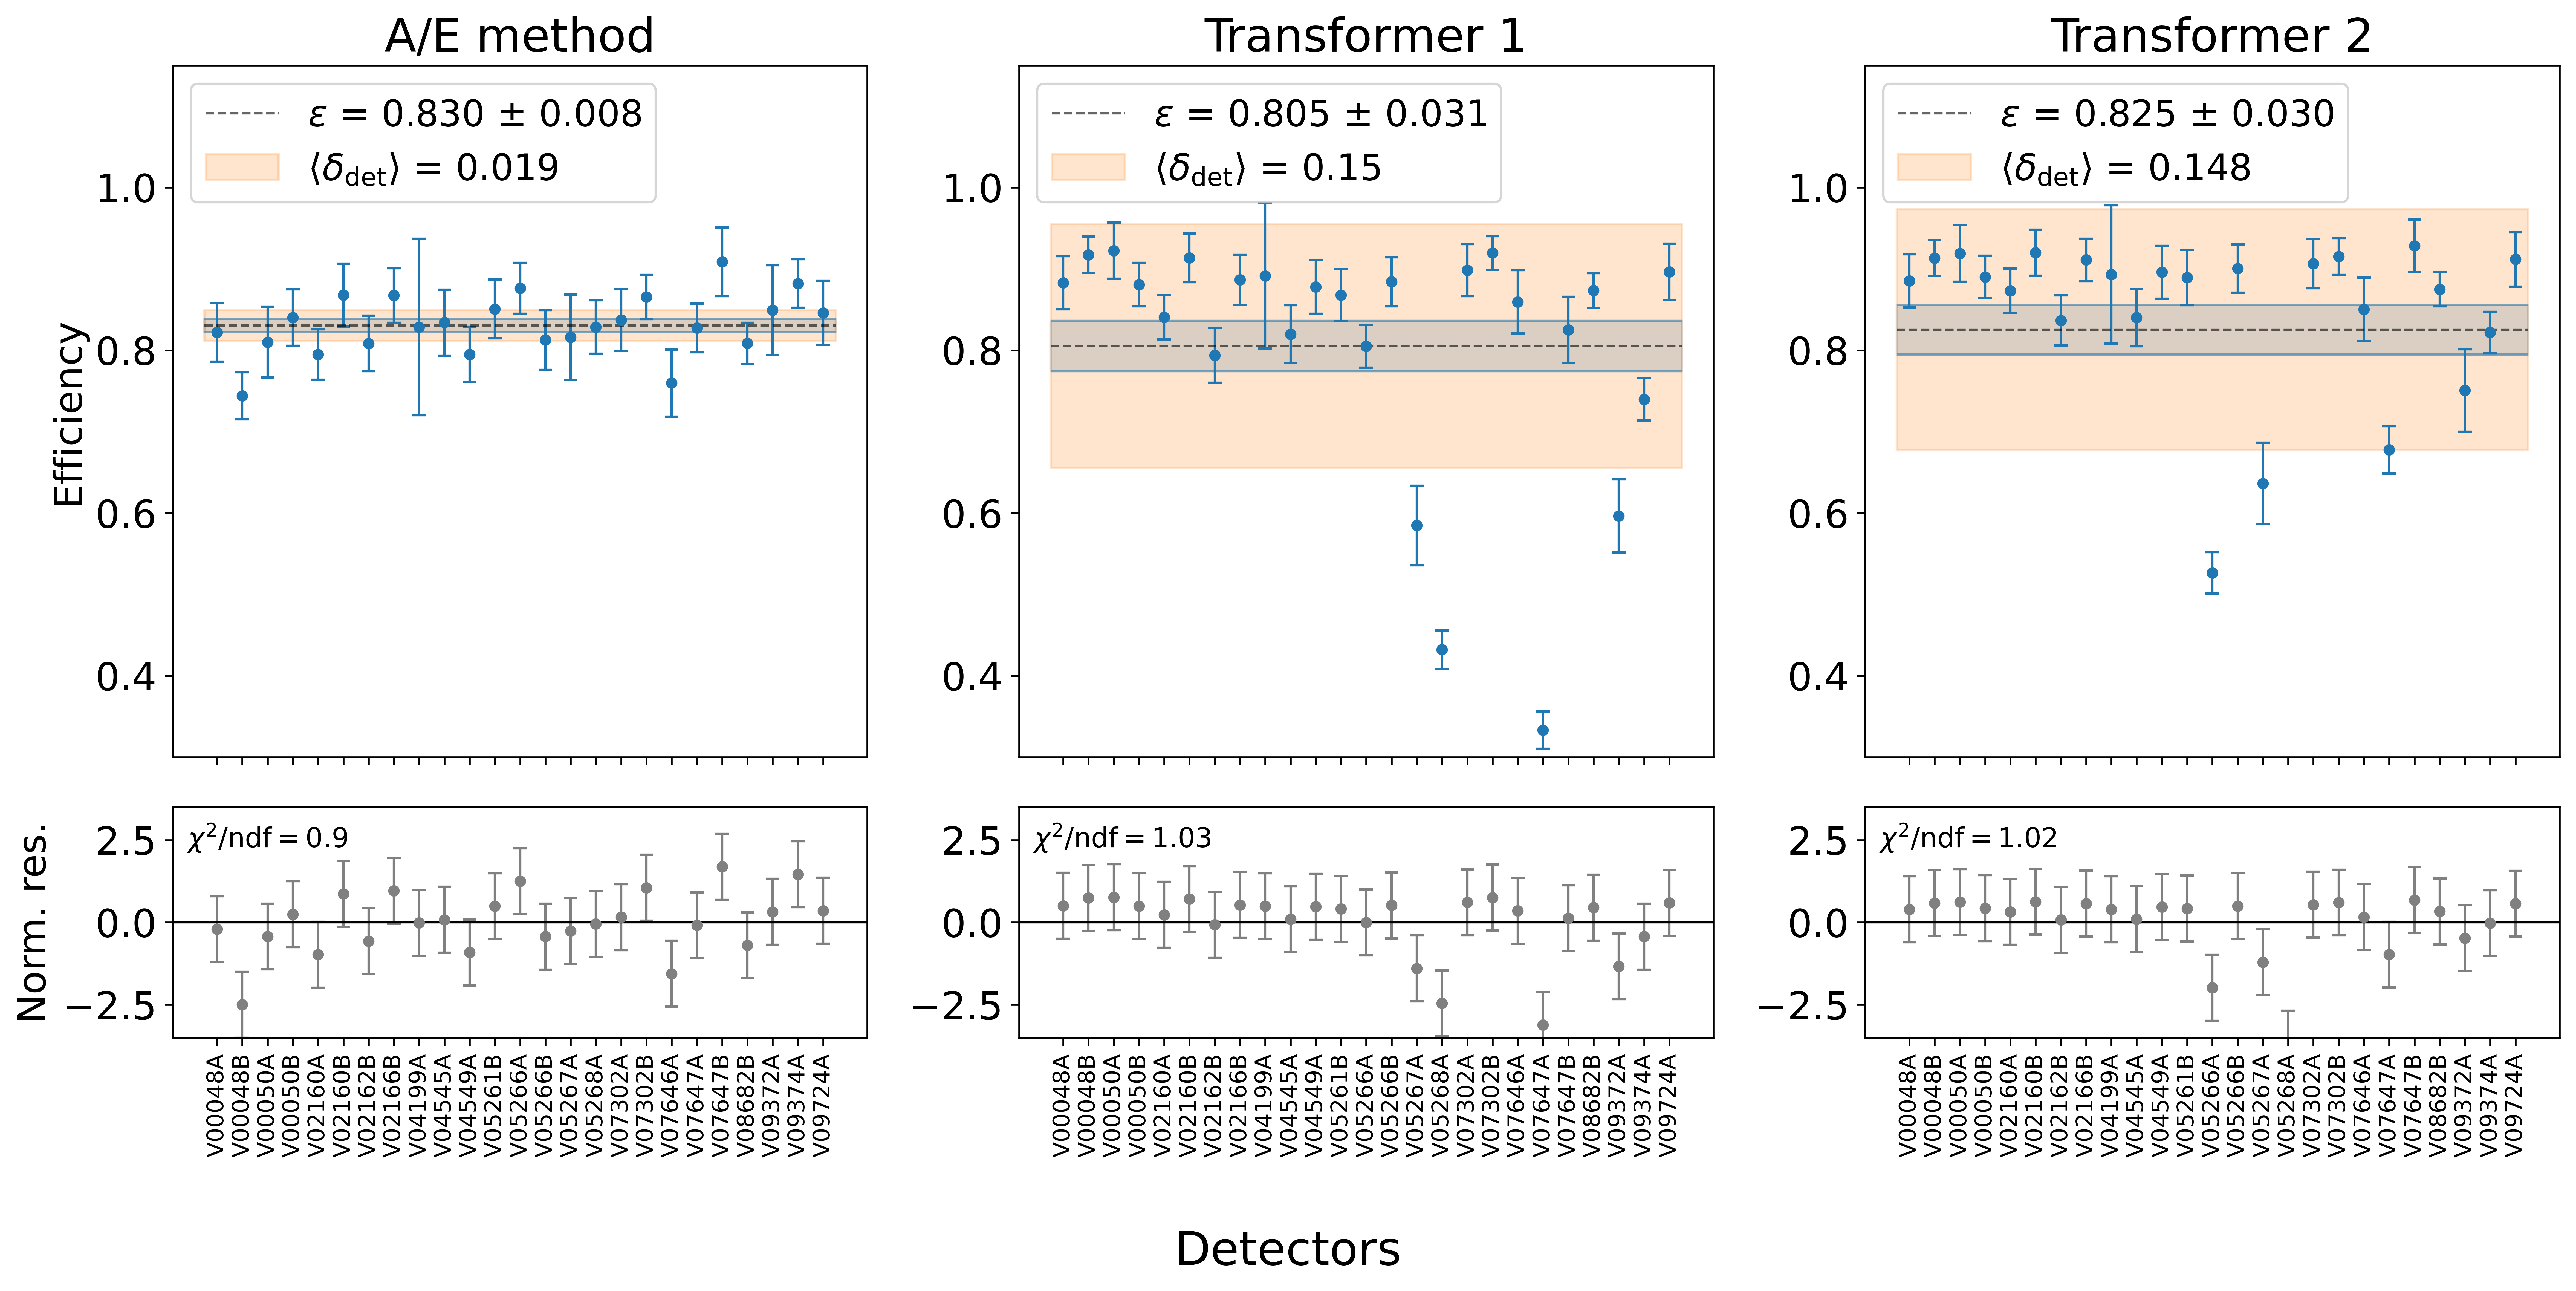
\includegraphics[width=\linewidth]{figures/05_PSD/PSD_eff_DEP_Co_new.png}
    \caption{PSD efficiencies in the $^{56}$Co DEP (2231.5~keV) for Mirion detectors used in this analysis. The efficiency is indicated by the blue band and the detector-to-detector uncertainty by the orange band. The Transformer models show less robustness compared to the A/E method when applied to this DEP. In several detectors, the Transformer classification fails completely. Possible causes include detector-specific waveform variations not captured in training or sensitivity to isotope-dependent event topologies, leading to significantly increased uncertainty. The lower panel shows the normalized residuals, demonstrating the quality of the fit. } 
\label{fig:psd_dep_Co}
\end{figure} 

\begin{table}
\centering
\caption{Additional uncertainty representing unaccounted detector-to-detector variations at the $^{208}$Tl and $^{56}$Co DEPs, and the systematic run-to-run variation. The PSD performance at the $^{208}$Tl DEP exhibits some spread ($< 4\%$). While the efficiency is very stable over time ($< 1\%$ for all models), the Transformer models show a very large detector-to-detector variation.}
\begin{tabular}{||c | c | c | c ||}
	\hline
 	\textbf{Quantity}  & \textbf{A/E [\%]} & \textbf{Model 1 [\%]} & \textbf{Model 2 [\%]} \\
 	\hline
    $\langle \delta_{\mathrm{det}} \rangle$ ($^{228}$Th) & 1.6 & 3.3 & 3.5  \\
 	\hline
 	$\langle \delta_{\mathrm{det}} \rangle$ ($^{56}$Co) & 1.9 & 15.0 & 14.8 \\
    \hline
 	$\langle \delta_{\mathrm{run}} \rangle$ & 0.8 & 0.6 & 0.9 \\ 
    \hline
\end{tabular}
\label{tab:fit_variances}
\end{table}

\subsubsection{Time dependence}

To estimate how the PSD efficiency varies over time across different data-taking periods, we repeat the procedure explained in the previous section. Instead of grouping the data by detector, we now group it by run. Each subset thus contains events from all detectors used in the analysis during that run. 
We then fit the efficiency data per run using the same statistical model, but we reinterpret the additional uncertainty term. In equation~\refeq{eq:chi2_eff_fit}, the detector-specific term $\langle \delta_{\mathrm{det}} \rangle$ is replaced by a run-specific term $\langle \delta_{\mathrm{run}} \rangle$, which quantifies the spread in the efficiencies due to potential time-dependent effects, such as drifts in detector response, electronic noise variations, or changes in environmental conditions.

\begin{equation}
\label{eq:chi2_eff_fit_time}
	\chi^2(\epsilon_i, \sigma_{\epsilon, i} \mid \langle \epsilon \rangle, \langle \delta_{\text{run}} \rangle) =
	\sum_i \left[ \frac{(\epsilon_i - \langle \epsilon \rangle)^2}{\sigma_{\epsilon,i}^2 + \langle \delta_{\text{run}} \rangle^2} + \log(\sigma_{\epsilon,i}^2 + \langle \delta_{\text{run}} \rangle^2) \right] \,.
\end{equation}

This approach allows us to quantify any systematic run-to-run variations in the PSD efficiency. The PSD efficiencies are illustrated in figure~\ref{fig:psd_timevar}, the spread due to time-dependent effects is shown in table~\ref{tab:fit_variances}. 


\begin{figure}
    \centering
    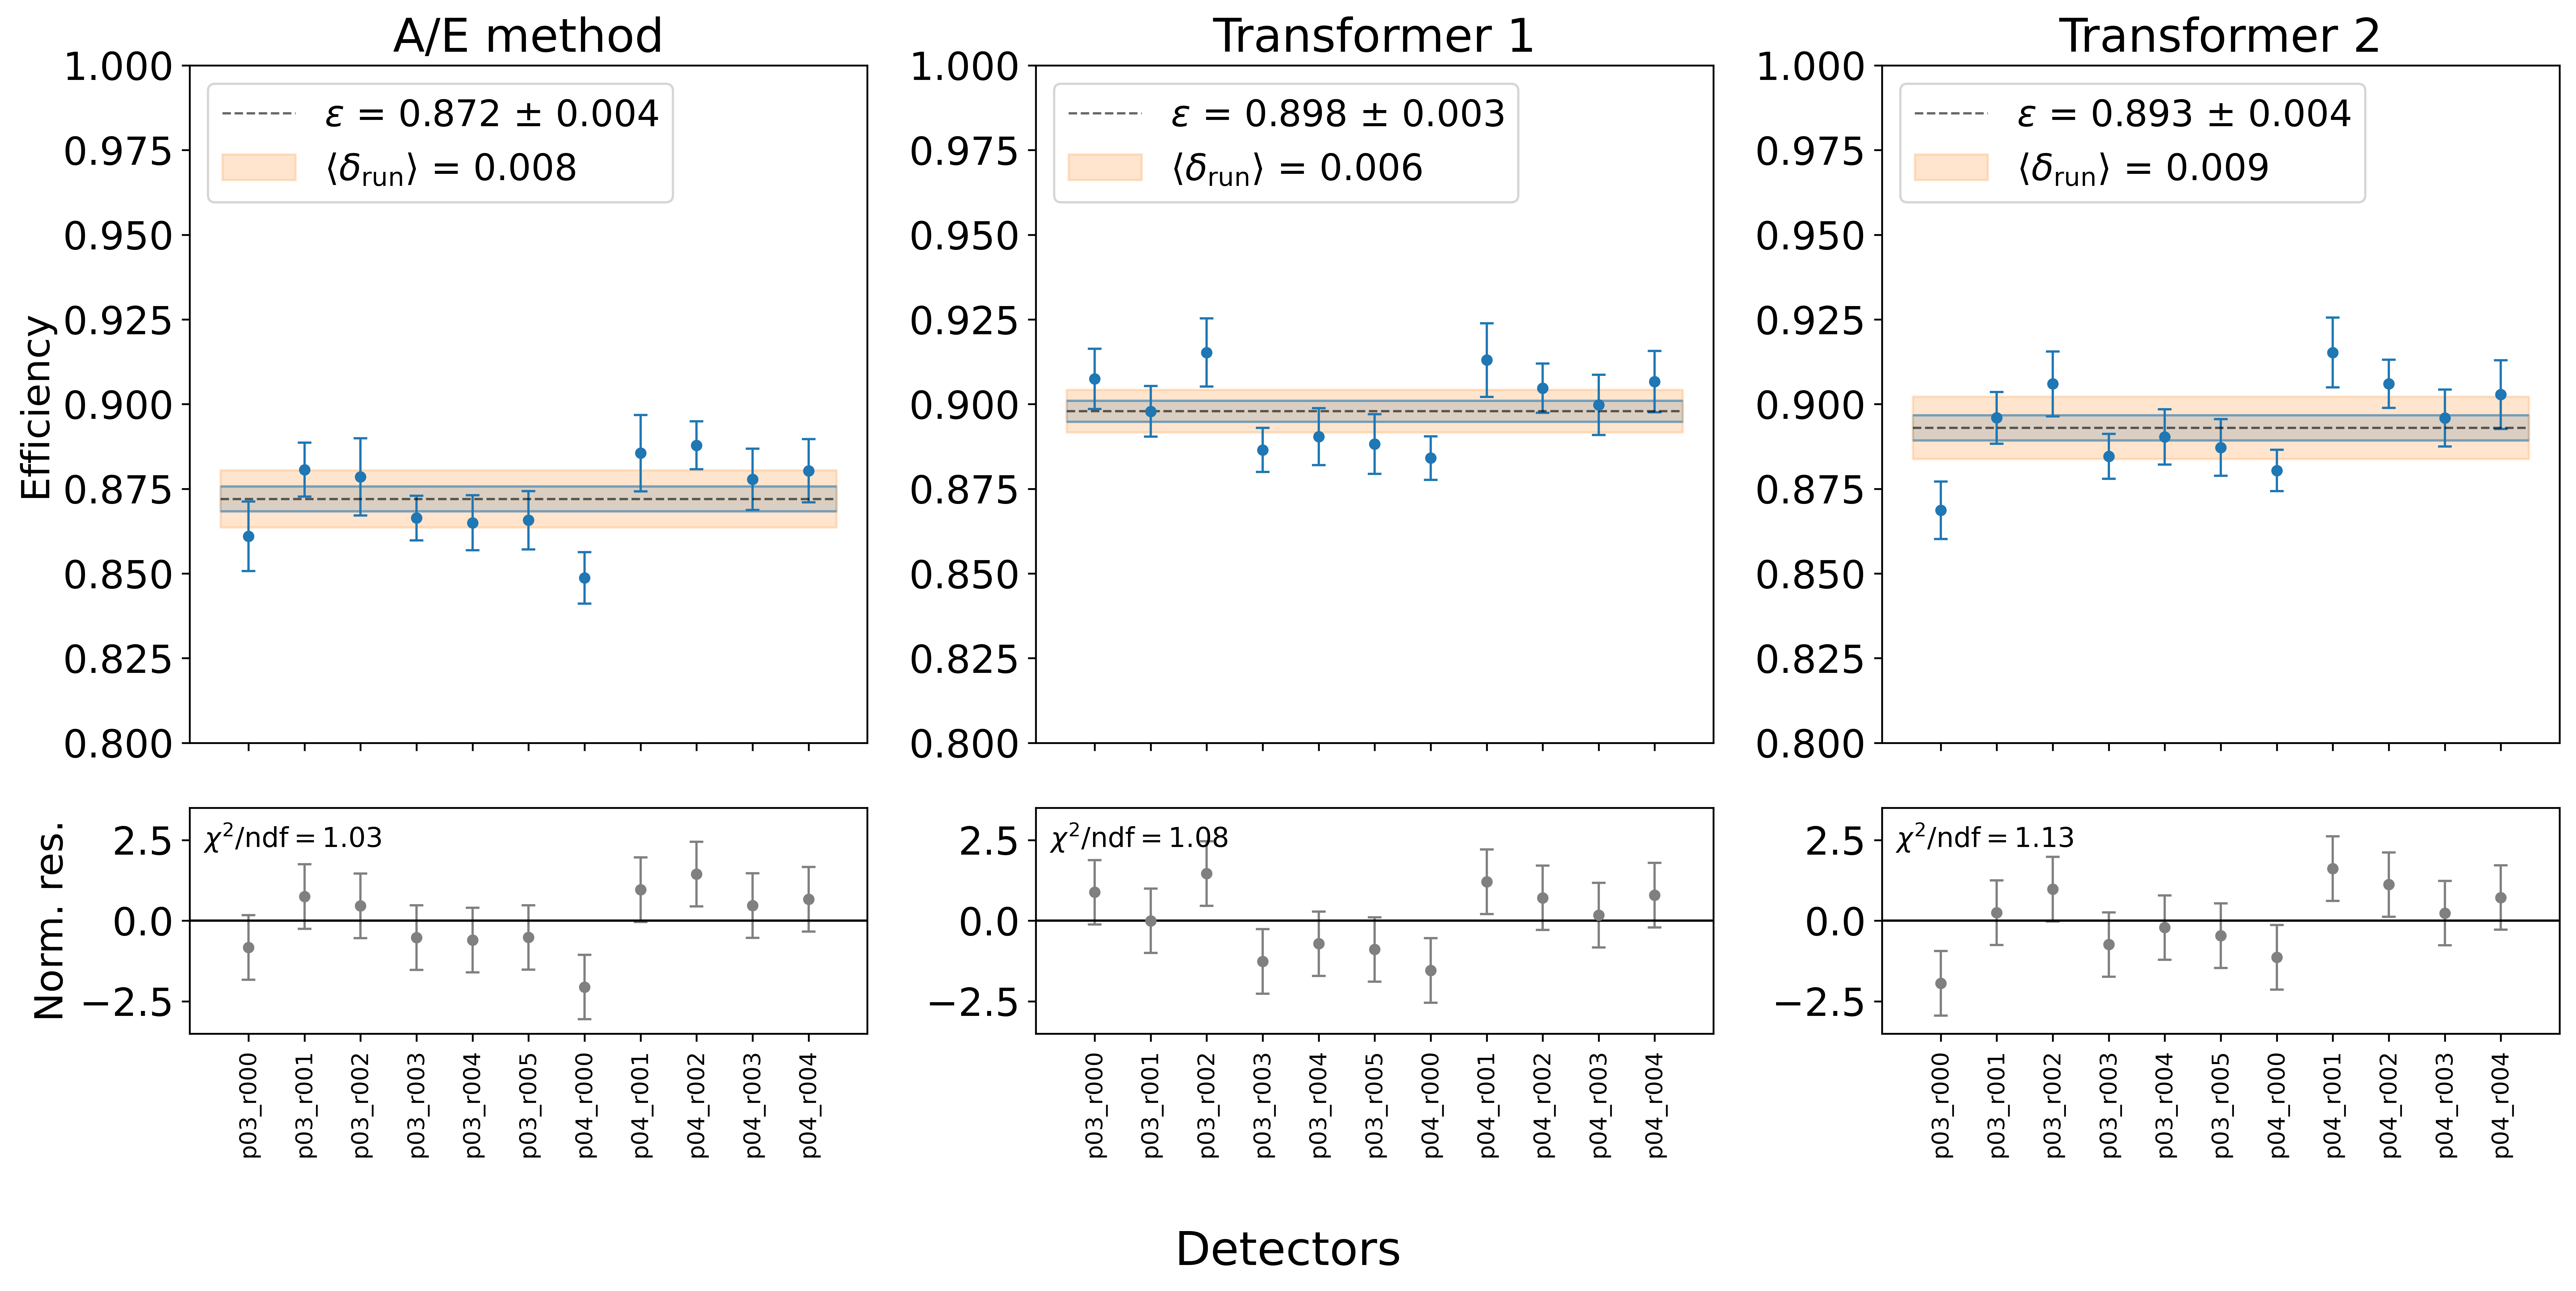
\includegraphics[width=\linewidth]{figures/05_PSD/PSD_eff_timevar_new.png}
    \caption{Time stability of the PSD efficiency (blue band) in the $^{208}$Tl DEP, shown per run for all detectors used. The efficiency remains very stable over time, and there is very little time-dependent uncertainty ($< 1\%$ throughout all models). The bottom panel shows the normalized residuals. }
\label{fig:psd_timevar}
\end{figure}



\subsubsection{Combined efficiency at \texorpdfstring{$Q_{\beta \beta}$}{}}

Although the $^{56}$Co source produces several higher-energy DEPs, most exhibit limited statistics and are therefore not suitable for a reliable estimation of the PSD efficiency estimates. 
To estimate the PSD efficiency at the region of interest, $\epsilon_{Q_{\beta \beta}}$, we perform a linear fit to the PSD efficiencies measured at the three selected energy regions. This is shown in figure~\ref{fig:psd_eff_qbb}. The uncertainty is obtained by propagating the uncertainties from the fit parameters using the covariance matrix:

\begin{equation}
\label{eq:linear_with_unc}
	\sigma_{\epsilon_{Q_{\beta \beta}}} = J \cdot \mathrm{Cov} \cdot J^\intercal \, ,
\end{equation}

\noindent where $J = \left[ \frac{\partial y}{\partial a} \; \frac{\partial y}{\partial b}\right]$ is the Jacobian and $\mathrm{Cov}$ the covariance matrix of the fitted parameters. 


\begin{figure}
    \centering
    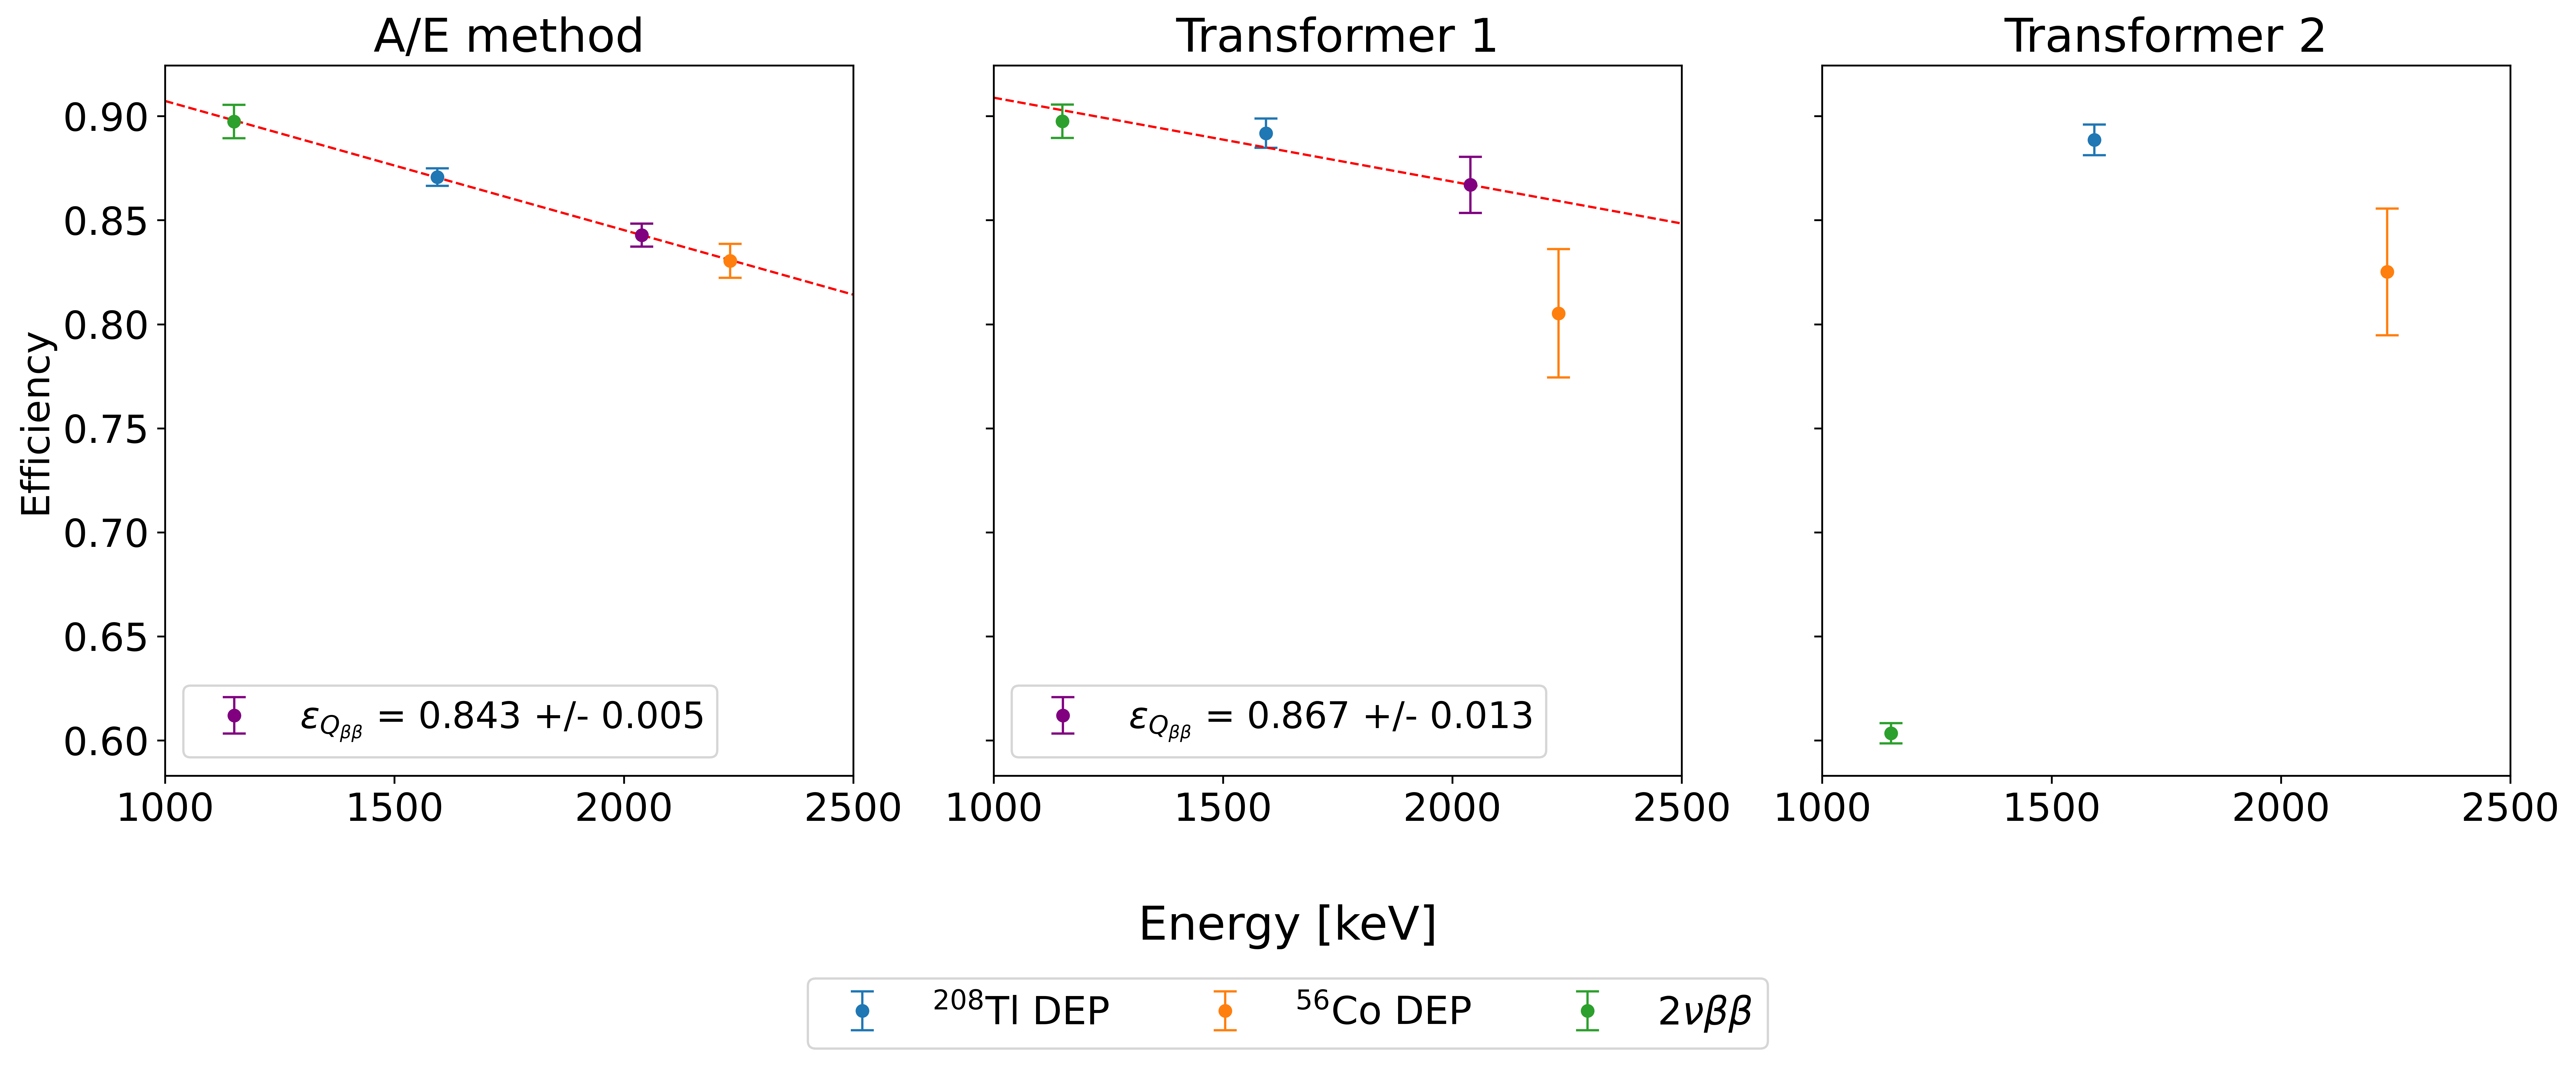
\includegraphics[width=\linewidth]{figures/05_PSD/PSD_eff_qbb.png}
    \caption{PSD efficiency as a function of energy for the three PSD methods. We evaluate the PSD efficiency at three different energies and extrapolate to $Q_{\beta \beta}$ using a linear fit. The A/E method is the most precise. The PSD efficiency of Transformer 1 is higher but exhibits a larger uncertainty. The Transformer model 2 failed for the $2 \nu \beta \beta$ decay events, which is why no fit was performed.}
\label{fig:psd_eff_qbb}
\end{figure}


The combined experimental efficiency of the experiment $\epsilon$, which enters the Bayesian fit as a nuisance parameter, includes also the liquid argon veto efficiency $\epsilon_{\mathrm{LAr}}$, the quality cut efficiency $\epsilon_{\mathrm{quality}}$, the fraction of active detector mass $\epsilon_{\mathrm{active}}$ and the $^{76}$Ge enrichment fraction $\epsilon_{\mathrm{Ge}}$. 
Therefore, the total experimental efficiency is given by:

\begin{equation}
\label{eq:total_efficiency}
	\epsilon = \epsilon_{\mathrm{PSD}} \cdot \epsilon_{\mathrm{LAr}} \cdot \epsilon_{\mathrm{quality}} \cdot \epsilon_{\mathrm{active}} \cdot \epsilon_{\mathrm{Ge}} \, .
\end{equation}

The associated uncertainty is estimated using Gaussian error propagation. Factoring out the total efficiency $\epsilon$, we find:  

\begin{equation}
\label{eq:total_efficiency_unc}
	\sigma_{\epsilon} = \epsilon \cdot \sqrt{ \sum_i \left( \frac{\sigma_{\epsilon_i}}{\epsilon_i} \right) } \, ,
\end{equation}

\noindent where the sum runs over all individual efficiency contributions listed above. The experimental efficiencies, not including PSD efficiencies, are summarized in table~\ref{tab:exp_effs}. These values were obtained from the LEGEND-200 internal metadata database, which is maintained by the collaboration and not publicly released. Efficiencies are provided for each detector and data-taking period; in this analysis, only periods 3 and 4 are used. For each efficiency type, the per-detector values were combined into a single number by taking the arithmetic mean, with the uncertainty given by the standard error of the mean.

\begin{table}
\centering
\caption{Summary of non-PSD experimental efficiencies in the range around $Q_{\beta \beta}$ used in this analysis. Values are taken from the LEGEND-200 internal metadata database for periods 3 and 4 only. For each efficiency type, the per-detector values were averaged, and the quoted uncertainty is the standard error of the mean across detectors.}
\begin{tabular}{||c | c ||}
	\hline
 	\textbf{Efficiency}  & \textbf{Value [\%]} \\
 	\hline
	Liquid Argon veto & $93 \pm 1$  \\
 	\hline
 	Quality cuts & $97.48 \pm 0.01$ \\
 	\hline
 	Active volume & $ 92.5 \pm 0.3 $ \\
 	\hline
 	$^{76}$Ge enrichment & $ 92.6 \pm 0.1$ \\
 	\hline
	Total (excluding PSD) & $77.7 \pm 0.9$ \\
	\hline
\end{tabular}
\label{tab:exp_effs}
\end{table}



\subsection{Pulse shape simulation}

The LEGEND-200 collaboration began developing a software package called LegendGeSim~\cite{noauthor_legend-explegendgesimjl_2025} with the goal of simulating detector waveforms for comparison studies with real data. 
This pulse shape simulation (PSS) framework is intended to support the validation of signal processing, and the goal was to use it to increase event classification across different energies. 
Written in Julia, LegendGeSim generates both idealized and partly realistic waveforms starting with a Geant4 simulation output. 
These results are stored in so-called PET files, which contain event position, energy and time information needed to simulate charge collection and signal formation in germanium detectors. The detector geometries required for these simulations are provided through metadata. 

The PET files are produced using ReMaGe, a modern \texttt{C\kern-.05em\texttt{++}} Geant4-based simulation framework for germanium experiments~\cite{pertoldi_remage_2025}. The geometries themselves are defined in the legend-pygeom-l200 package~\cite{noauthor_legend-explegend-pygeom-l200_2025}, developed within the LEGEND-200 collaboration. 
Finally, a dedicated interface script was developed to convert the Geant4 output into a format compatible with LegendGeSim. Additionally, a coordinate transformation is required, since ReMaGe and LegendGeSim use different coordinate systems\footnote{Credit to Giovanna Saleh for identifying and resolving this inconsistency.}.  

Figure~\ref{fig:PSS_diagram} illustrates the interaction between the various software components used in the waveform simulation pipeline. 

\begin{figure}
\centering
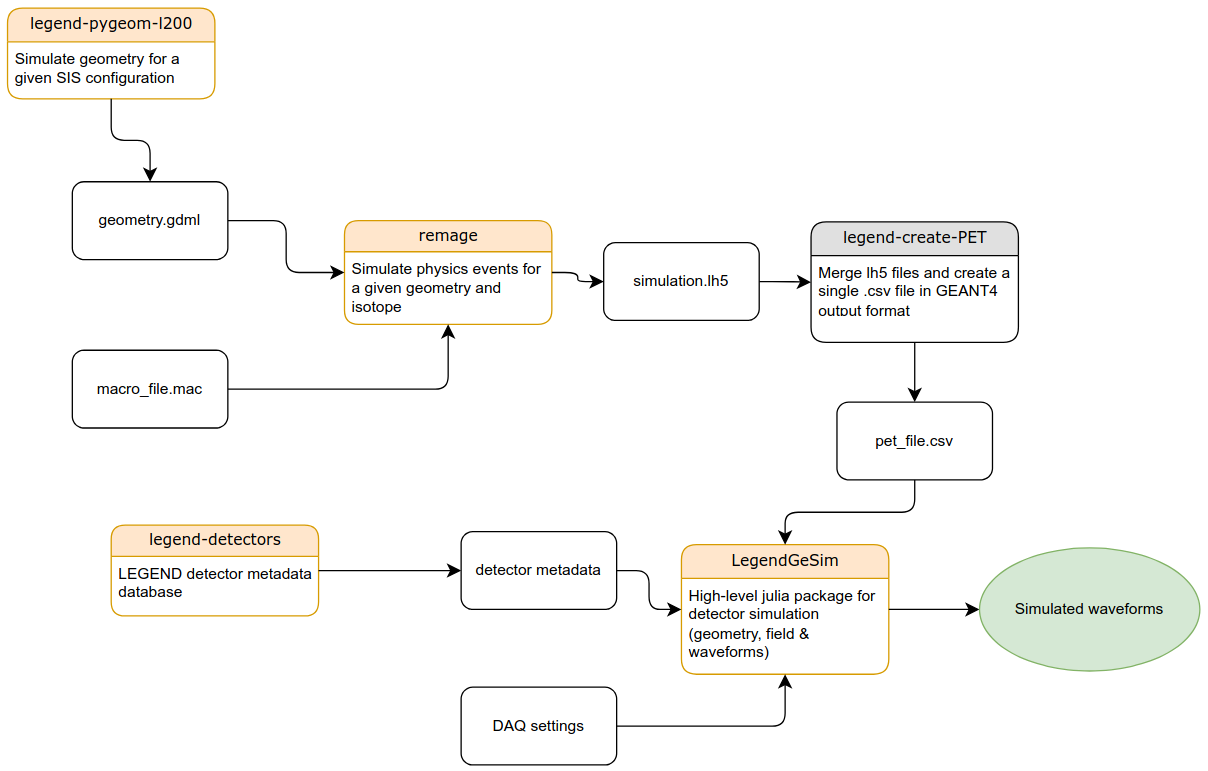
\includegraphics[width=\linewidth]{figures/05_PSD/PSS_diagram.png}
\caption{Connection between different LEGEND packages for the use of LegendGeSim.} 
\label{fig:PSS_diagram}
\end{figure}

Despite the promising concept, the LegendGeSim framework remains under development and is not yet fully functional. In attempting to use it, we encountered several limitations that hindered its use for this project: 
\begin{itemize}
\item \textbf{Incomplete physics modeling}: Essential mechanisms such as diffusion, charge cloud drift, charge trapping, and temperature dependence are either not fully implemented or not comparable with data.  
\item \textbf{Systematic uncertainties}: Systematics associated with different PSD parameters and the simulated electronics chain are not yet characterized. 
\item \textbf{Inaccurate energy reconstruction}: The trapezoidal filter used in the framework systematically underestimates the true energy of events. 
\end{itemize}

The inaccurate energy reconstruction is evident in figure~\ref{fig:PSS_histogram}, which compares simulated data to calibration measurements. Example waveforms are shown in figure~\ref{fig:PSS_waveforms}, where a systematic slowly rising current signal is visible.  

The current pulse shape simulation workflow suffers from significant inefficiency, with runtimes so long that large-scale waveform generation is impractical. 
A major bottleneck is that, in its present implementation, ReMaGe must fully simulate each event before deciding whether to retain it. Consequently, complete decay chains (e.g., the $^{228}$Th chain) are simulated, and the full energy spectrum is generated, including events outside the peaks of interest. 
There is the option to restrict the decay chain (e.g., to only $^{208} \mathrm{Tl} \rightarrow ^{208} \mathrm{Pb}$); this has to be handled with care, as it might introduce bias. While it is possible to apply generator-level energy cuts, this approach is non-trivial. These inefficiencies occur before the actual pulse-shape simulation in LegendGeSim. 
For the dataset shown in figure~\ref{fig:PSS_histogram}, the simulation required 27.5~hours of wall time on NERSC (using 128 CPU cores in parallel for ReMaGe only) for a single detector (V09372A), yielding approximately 5000 events in the $^{208}$Tl DEP.  

\begin{figure}
\centering
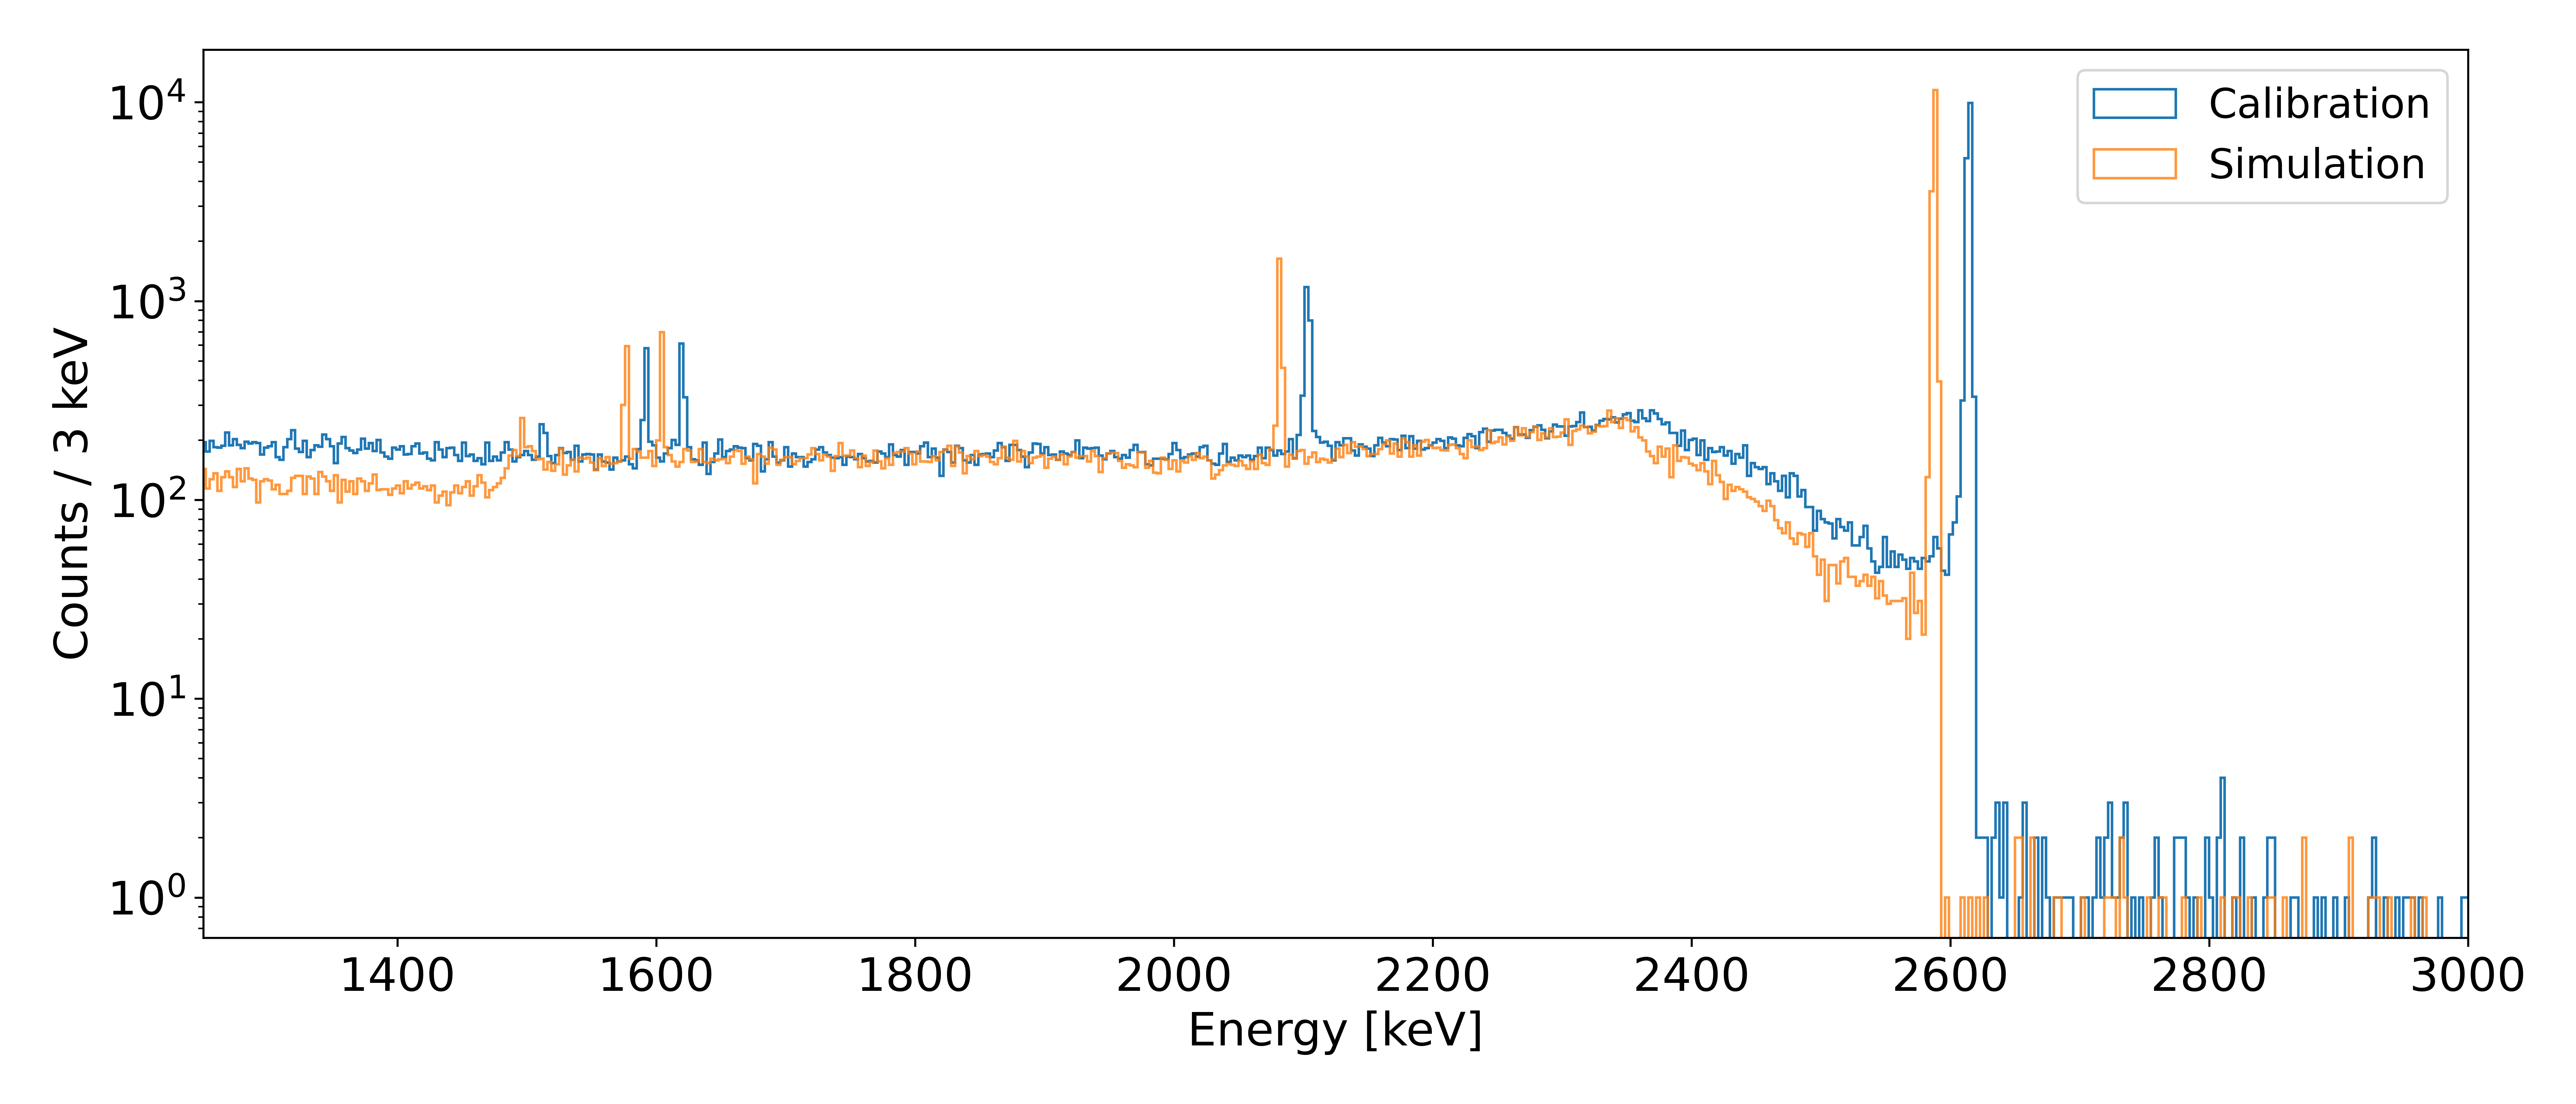
\includegraphics[width=\linewidth]{figures/05_PSD/Plot_cal_vs_PSS.png}
\caption{Energy spectrum for the IC detector V09372A, comparing calibration data (blue) from period 3 with simulated data (orange). In the simulation, the decay chain is restricted to nuclei with $208 \leq A \leq 212$ and $81 \leq Z \leq 83$, and only events with energies above 1200~keV are retained. The simulated spectrum shows a systematic shift of the characteristic $\gamma$-lines toward lower energies, indicating inaccuracies in the energy reconstruction.}
\label{fig:PSS_histogram}
\end{figure}

\begin{figure}
\centering
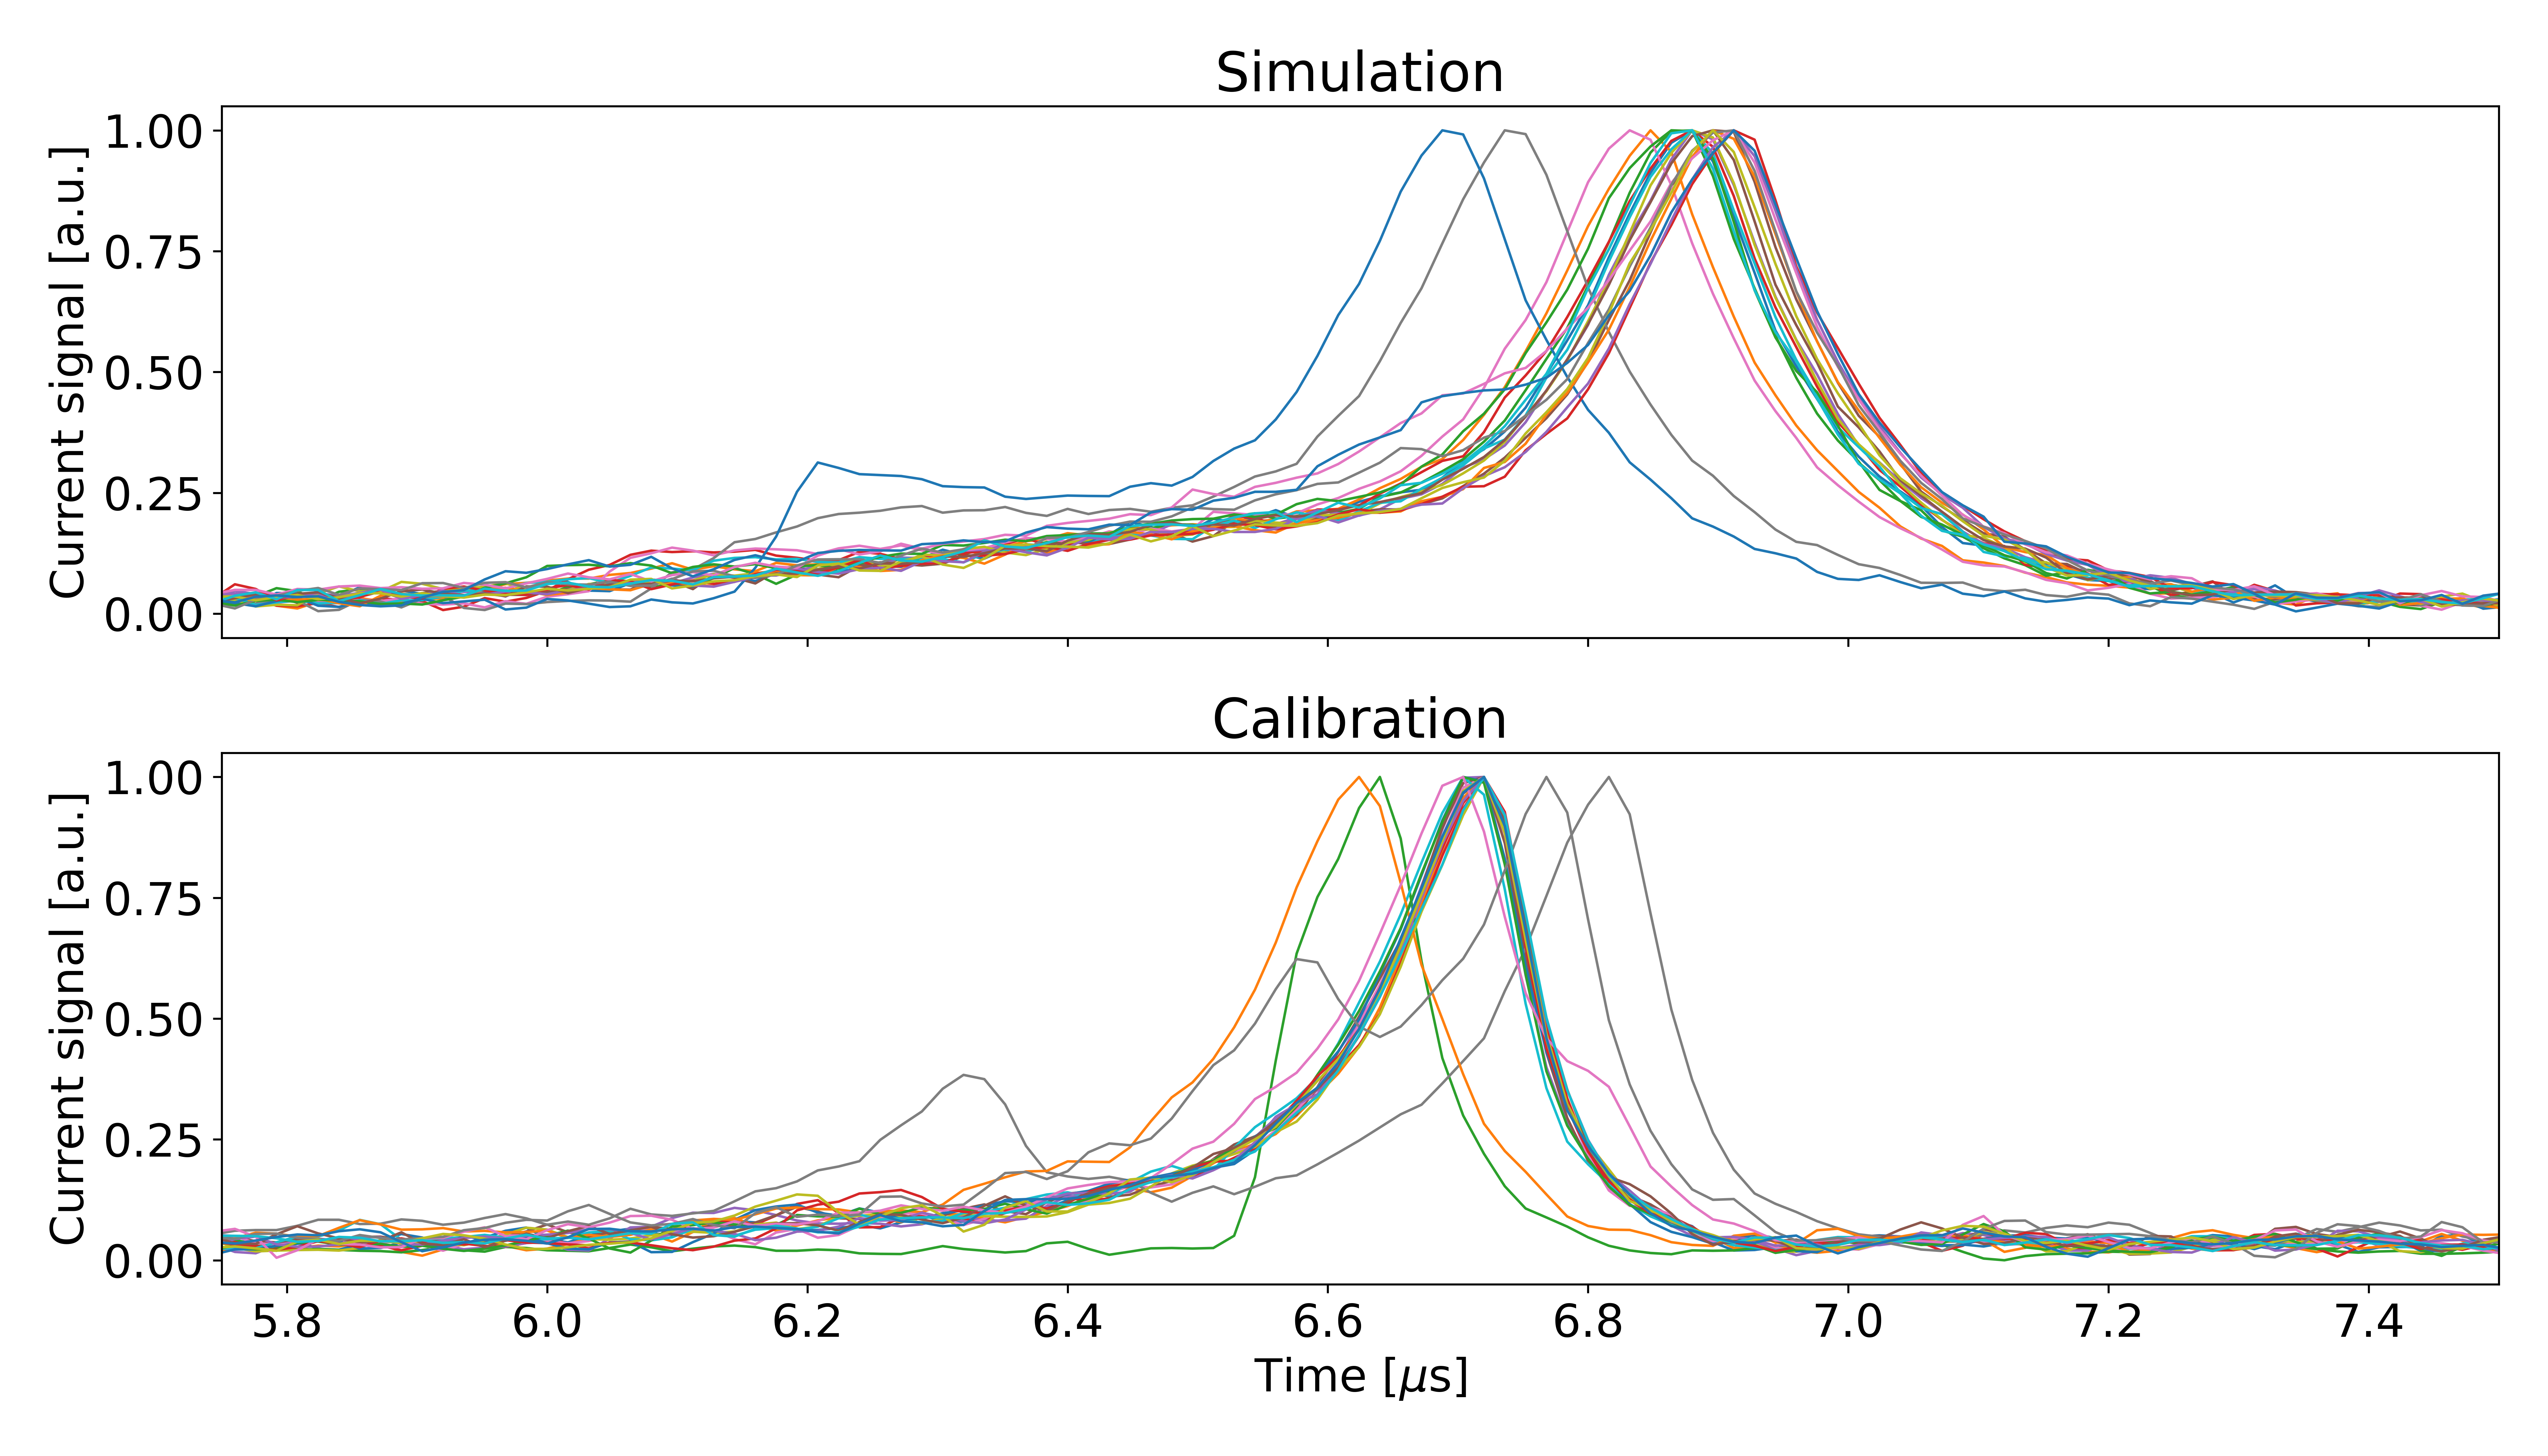
\includegraphics[width=\linewidth]{figures/05_PSD/Plot_waveform_cal_vs_pss.png}
\caption{Example waveforms for the IC detector V09372A in the $^{208}$Tl DEP at 1592.5~keV, comparing simulated waveforms (top panel) with calibration data from period 3 (bottom panel). The simulated waveforms exhibit a systematically slower, early rise compared to the measured data. }
\label{fig:PSS_waveforms}
\end{figure}

The Pulse Shape Simulation (PSS) framework was expected to serve as a practical tool for this study. 
Although some development work was anticipated, the framework turned out to be less mature and more complex to integrate than expected. 
At the time of writing, further development is ongoing within the LEGEND-200 collaboration, with significant contributions from the University of Zurich.
Nonetheless, this work established a functioning processing pipeline for handling simulated PSS data from a single detector. 
Due to time constraints, a full-scale simulation was not achieved, but the essential tools required for generating, processing, and analyzing simulated waveforms are now in place for use in future studies. 




\subsection{Summary and combined results at \texorpdfstring{$Q_{\beta \beta}$}{}}

In this work, a Transformer-based PSD method for the LEGEND-200 experiment was developed. Of the three transformer models tested, only Transformer model 1 demonstrated stable and reliable performance across the full energy range. The PSD efficiency at $Q_{\beta \beta}$ was obtained by interpolating between three reference points: $2 \nu \beta \beta$ decay events in the 1000-1300~keV interval, the 1592.5~keV DEP of $^{208}$Tl, and the 2231.5~keV DEP of $^{56}$Co. Additional systematic uncertainty was included to account for time-dependent stability, detector-to-detector variations, and differences in PSD acceptance between $2 \nu \beta \beta$ and DEP events. The final PSD efficiency yields $(86.7 \pm 1.3)$\% at $Q_{\beta \beta}$ for the Transformer. This is consistent with the efficiency obtained by the conventional A/E method, $(84.3 \pm 0.5)$\%, with a two-sided p-value of $p = 0.08$ indicating no significant difference between the two approaches at the 5\% level. 
Taking into account the experimental efficiencies listed in table~\ref{tab:exp_effs}, the overall detection efficiency achieved with the Transformer-based approach is $(66.8 \pm 2.1)$\%, compared to $(65.0 \pm 2.0)$\% for the A/E method.  


%--------------------- Sensitivity study ---------------------
\clearpage
\section{Sensitivity study for the \texorpdfstring{$0 \nu \beta \beta$ decay}{}}
\label{sec:06_Sensitivity}
Bayesian statistics offers a powerful framework for modeling uncertainty and performing probabilistic inference, making it particularly well-suited for rare-event searches such as $0 \nu \beta \beta$ decay. 
In this chapter, we explain the essential principles of Bayesian inference and present the statistical model used to estimate the experimental sensitivity for $0 \nu \beta \beta$ decay discovery under a background-only hypothesis and varying pulse shape discrimination efficiencies. 
We do not apply the likelihood model (equation~\refeq{eq:bayes_likelihood}) directly to real data. Although the LEGEND-200 data in the $(Q_{\beta \beta} \pm 25)$~keV window has been unblinded, waveform-level information is not accessible to the full collaboration. Instead, we estimate the expected 90\% credible upper limit on the signal half-rate, defined as the inverse of the signal half-life (see equation~\refeq{eq:signal_half_rate}), using toy Monte Carlo datasets. The usage of half-rate $\mathcal{S} = 1 / T^{0 \nu}_{1/2}$ instead of half-life improves numerical stability. 
To this end, we generate toy spectra and fit them using a signal-plus-background model within a Markov Chain Monte Carlo framework. From the resulting posterior distributions, we derive upper limits on the signal half-rate and define the experimental sensitivity as the median of the 90\% credible interval (CI) distributions. We also detail the fit procedure, including the treatment of nuisance parameters. 


\subsection{Introduction to Bayesian inference}

Bayes' theorem forms the foundation of Bayesian inference, providing a formal mechanism for updating probabilistic beliefs based on observed data:

\begin{equation}
\label{eq:bayes_theorem}
	p(\boldsymbol{\theta} \mid \mathrm{data}) = \frac{p(\mathrm{data} \mid \boldsymbol{\theta}) \cdot p(\boldsymbol{\theta})}{p(\mathrm{data})} \,.
\end{equation}

\noindent Here, $p(\boldsymbol{\theta})$ denotes the prior distribution, which encodes our prior knowledge or assumptions about the parameters before observing any data. The likelihood $p(\mathrm{data} \mid \boldsymbol{\theta})$ quantifies how probable the observed data is under a given choice of parameters. The resulting posterior distribution $p(\boldsymbol{\theta} \mid \mathrm{data})$ reflects the updated knowledge after accounting for the observed data. If the parameters $\boldsymbol{\theta} = (\theta_1, \theta_2, \ldots, \theta_n)$ are independent, the posterior becomes:

\begin{equation}
\label{eq:bayes_theorem_indep}
	p(\boldsymbol{\theta} \mid \mathrm{data}) = \frac{p(\mathrm{data} \mid \boldsymbol{\theta}) \cdot \prod_{i=1}^n p(\theta_i)} {p(\mathrm{data})} \,.
\end{equation}

This factorization is an approximation that holds only if the parameters are uncorrelated under the prior. In practice, some parameters may exhibit correlations, and modeling their joint prior distribution may be necessary to accurately capture posterior dependencies.
The normalization factor, $p(\mathrm{data})$, known as marginal likelihood, ensures the posterior is normalized:

\begin{equation}
\label{eq:bayes_theorem_normalization}
	p(\mathrm{data}) = \int_{\theta} p(\theta) p(\mathrm{data} \mid \theta) \, d\theta \,.
\end{equation}

This integral marginalizes over all possible values of $\theta$, weighted by their prior probabilities. Marginalization is particularly useful to extract the distribution for a given parameter by integrating out the joint distribution over the unknowns that are not of interest. We later apply it to remove nuisance parameters -- quantities that affect the model but are not of direct interest~\cite{gelman_bayesian_2014}. 

Once the posterior distribution is obtained, it can be used to make predictions about new or unseen data via the posterior predictive distribution. It describes the distribution of potential future observations from a repeated experiment conducted under identical conditions:

\begin{equation}
	p(y \mid \mathrm{data}) = \int p(y, \theta \mid \mathrm{data}) \, d\theta = \int p(y \mid \theta) p(\theta \mid \mathrm{data}) \, d\theta \,.
\end{equation}

\noindent Here, $y$ represents a hypothetical data, $\theta$ are the model parameters, and $p(y \mid \theta)$ is the likelihood of observing $y$ given those parameters. The posterior distribution $p(\theta \mid \mathrm{data})$ captures what we have learned about $\theta$ from the observed data.  

Posterior predictive studies are particularly useful for model checking and sensitivity analysis, as they naturally incorporate uncertainty in the model parameters. They are often used to compare the posterior predictive distribution to newly observed data, because this provides insight into how the model and prior assumptions align with reality. If the original data were modeled appropriately, then the generated values of $y$ under the model should exhibit a distribution similar to that of the observed data.


\subsection{Statistical model for sensitivity estimation}
\label{sec:05_stat_model}


To evaluate the effect of the different PSD efficiencies on the half-life sensitivity of the $0 \nu \beta \beta$ decay, we perform a Bayesian sensitivity study using toy Monte Carlo datasets generated under the null hypothesis (background-only scenario). The $0 \nu \beta \beta$ decay analysis is performed over the energy range from 1930 to 2190~keV. 
Two $\gamma$-lines at $(2104 \pm 5)$~keV and $(2119 \pm 5)$~keV are excluded, resulting in a net analysis window of 240~keV~\cite{gerda_collaboration_final_2020}. The expected number of $0 \nu \beta \beta$ decay events in toy MC datasets, as a function of the signal half-rate $\mathcal{S} = 1/T^{0 \nu}_{1/2}$, is given by:


\begin{equation}
\label{eq:0vbb_signal_counts}
	s \left( \mathcal{S} \right) =  \frac{\log{2} \cdot \mathcal{E} \cdot N_A \cdot \epsilon}{m_{\mathrm{mol}}} \cdot \mathcal{S} = \frac{\log{2} \cdot \mathcal{E} \cdot N_A \cdot \epsilon}{m_{\mathrm{mol}}} \cdot \frac{1}{T_{1/2}} \,.
\end{equation}

Here, we have the following parameters~\cite{agostini_background-free_2017}:

\begin{itemize}
    \item $\mathcal{E} = 1000 \;\mathrm{kg} \cdot {\mathrm{yr}}$ is the exposure
    \item $N_A = 6.022 \times 10^{23} \; \mathrm{mol}^{-1}$ is Avogadro's number
    \item $\epsilon$ is the detection efficiency, calculated as in equation~\refeq{eq:total_efficiency}
    \item $m_{\mathrm{mol}} = 75.92$ g/mol is the molar mass of $^{76}$Ge 
    \item $T^{0 \nu}_{1/2}$ is the $0 \nu \beta \beta$ decay half-life
\end{itemize}

\noindent The number of background events $b$ is given by:


\begin{equation}
\label{eq:0vbb_background_counts}
	b \left( \mathcal{B} \right) = \mathcal{E} \cdot \Delta E \cdot \mathcal{B} \,,
\end{equation}

\noindent where $\Delta E = 240$ keV is the net width of the energy window used for the fit and $\mathcal{B}$ the background index in counts/(keV$\cdot$kg$\cdot$yr). 
Assuming a counting experiment with a total of $n$ observed events surviving the analysis cuts in the analysis window, the full unbinned extended likelihood takes the form:

\begin{equation}
\label{eq:bayes_likelihood}
	L \left( \mathrm{data} \mid \mathcal{S}, \; \mathcal{B}, \; \vartheta \right) = \frac{(s+b)^n \cdot e^{-(s+b)}}{n!} \cdot \prod_i^n \left[ \frac{1}{s+b}  \Big( s \cdot p_s(E_i) + b \cdot p_b \Big)  \right]
\end{equation}

The first factor is the Poisson probability of observing $n$ events given the total expected rate $s + b$, while the product accounts for the probability density functions of each event's energy $E_i$, normalized over signal and background contributions. Further, $\vartheta$ denotes the nuisance parameters. In this analysis, the signal distribution $p_s(E)$ is modeled as a Gaussian centered at the decay Q-value, which is valid if we assume negligible detector-specific non-Gaussian tails or energy leakage. The background distribution $p_b(E)$ is modeled as flat across the analysis window: 

\begin{align}
\label{eq:bayes_sig_pdf}
	p_s(E) & = \frac{1}{\sqrt{2 \pi} \sigma} \cdot e^{-\frac{ \left(E - x\right)^2}{2 \sigma^2}} \,,\\
	p_b & = \frac{1}{E_{\mathrm{max}} - E_{\mathrm{min}}}   \,,
\label{eq:bayes_bkg_pdf}
\end{align}

\noindent where $x = Q_{\beta \beta} - \Delta$ is the energy bias, with $\Delta = E_{\mathrm{true}} - E_{\mathrm{cal}}$. In addition, we consider two more nuisance parameters: the energy resolution $\sigma$ and the signal efficiency $\epsilon$. The prior distributions are modeled as Gaussian centered around their nominal values ($\hat{\sigma}$, $\hat{\epsilon}$, and $\hat{\Delta}$). Assuming the nuisance parameters to be independent, the joint prior distribution is:

\begin{align}
\label{eq:bayes_nuisance_parm}
	\mathcal{P}( \sigma, \epsilon, \Delta ) & = \mathcal{P}(\sigma) \cdot \mathcal{P}(\epsilon) \cdot \mathcal{P}(\Delta) \\
    & = 
	\frac{1}{\sqrt{2 \pi} \sigma_{\sigma}} \cdot e^{-\frac{\left( \sigma - \hat{\sigma} \right)^2}{2 \sigma_{\sigma}^2}} \cdot 
	\frac{1}{\sqrt{2 \pi} \sigma_{\epsilon}} \cdot e^{-\frac{\left( \epsilon - \hat{\epsilon} \right)^2}{2 \sigma_{\epsilon}^2}}  \cdot
    \frac{1}{\sqrt{2 \pi} \sigma_{\Delta}} \cdot e^{-\frac{\left( \Delta - \hat{\Delta} \right)^2}{2 \sigma_{\Delta}^2}}  \nonumber \,.
\end{align}

Here, $\sigma_\vartheta$ is the standard deviation of the respective prior, which quantifies the uncertainty in the measurements. For the signal half-rate $\mathcal{S}$ and the background index $\mathcal{B}$, we use uniform priors over physically allowed ranges, which are $[0, 1000] \times 10^{27} \; \mathrm{yr}^{-1}$ for $\mathcal{S}$ and $[0, 0.1]$~counts/(keV$\cdot$kg$\cdot$yr) for the background index. 
Applying Bayes' theorem, the posterior probability density becomes: 


\begin{align}
	p\left( \mathcal{S}, \; \mathcal{B}, \; \sigma, \: \epsilon, \; \Delta \mid \mathrm{data} \right) & \propto \; 
	L \left( \mathrm{data} \mid \mathcal{S}, \; \mathcal{B}, \; \sigma, \; \epsilon, \; \Delta \right) \\ & \times  \mathcal{P}(\sigma, \epsilon, \Delta) \cdot \mathcal{P}(\mathcal{S}) \cdot  \mathcal{P}(\mathcal{B})  \nonumber \,.
\end{align}

This formulation enables the systematic propagation of uncertainties in resolution and efficiency to the final inference on the signal half-rate and background index. In general, the marginalization over nuisance parameters cannot be solved analytically. Therefore, we perform the integration numerically using a Markov chain Monte Carlo (MCMC) approach. Specifically, we employ the Metropolis-Hastings sampling algorithm to generate samples from the posterior distribution. For this analysis, we use 5 independent MCMC chains, each with $10^{5}$ sampling steps. Multiple MCMC chains are employed to mitigate the dependence of finite-length chains on their initial values, thereby enhancing the reliability of the resulting estimates.


\subsection{Toy Monte Carlo simulations}

The procedure for the generation and analysis of toy datasets is as follows. 
First, we sample nuisance parameters. For each toy dataset, the signal detection efficiency $\epsilon$ and the energy resolution $\sigma$ are drawn from their respective priors. Since only Mirion ICPC detectors are considered in this analysis, we achieve an excellent energy resolution of $\sigma = (0.914 \pm 0.062)$~keV. Furthermore, $\Delta$ was set to zero, neglecting a potential energy bias. This is in agreement with the recently published first results from the LEGEND-200 experiment, which show an energy bias of $(0.3 \pm 0.3)$~keV for ICPC detectors~\cite{legend200_fist_results_2025}. In that analysis, an energy-bias correction was applied; however, the fitted bias was consistent with zero within uncertainties.

In the second step, we generate the number of events. The total number is drawn from a Poisson distribution, with an expected mean determined by the assumed background index, as shown in equation \refeq{eq:0vbb_background_counts}. To determine the final experimental sensitivity of LEGEND-200, we use the background goal of $\mathcal{B} = 2 \cdot 10^{-4}$ counts/(keV$\cdot$kg$\cdot$yr). 
Finally, we construct the toy spectrum: assuming background-only, event energies are sampled from the background probability density function $p_b(E)$. 

Each toy dataset is then analyzed using the full signal-plus-background likelihood model defined in section~\ref{sec:05_stat_model}. To extract the 90\% CI upper limit $\mathcal{S}_{90}$ on the signal half-rate, we first marginalize the joint posterior over all other parameters:

\begin{equation}
\label{eq:Bayesian_marginalization}
    p(\mathcal{S} \mid \mathrm{data}) = \int p(\mathcal{S}, \mathcal{B}, \sigma, \epsilon, \Delta \mid \mathrm{data}) \; d \mathcal{B} \, d \sigma \, d \epsilon \,.
\end{equation}

The 90\% CI upper limit is then given by:

\begin{equation}
\label{eq:Bayesian_S_90}
    \int_0^{\mathcal{S}_{90}} p\left( \mathcal{S} \mid \mathrm{data} \right) \; d\mathcal{S} = 0.9 \,.
\end{equation}



This procedure is repeated for $10^{4}$ independent toy datasets. This number ensures statistical robustness of the $\mathcal{S}_{90}$ distribution and smooth convergence of CI estimates. The median of $\mathcal{S}_{90}$, denoted $\tilde{\mathcal{S}}_{90}$, serves as the expected upper limit on the signal half-rate for repeated experiments under the same conditions. This can be translated into a lower bound on the $0 \nu \beta \beta$ decay half-life. 

\begin{figure}
\centering
\includegraphics[width=\linewidth]{figures/06_sensitivity/signal_fit_per_toy_1000kgyr.png}
\caption{Scatter plots (top) and distributions (bottom) for the best-fit signal half-rate $\mathcal{S}$ obtained from MCMC fits to $10^{4}$ toy Monte Carlo datasets generated under the background-only hypothesis. The A/E method (left) and the Transformer-based PSD method (right) correspond to different assumed PSD efficiencies in the toy generation. Both yield similar results, with the majority of toys returning $\mathcal{S} = 0$, because no events fall within the signal region around $Q_{\beta \beta}$. Non-zero $\mathcal{S}$ values arise when background fluctuations place one or more events close to $Q_{\beta \beta}$, producing discrete populations at characteristic $\mathcal{S}$ levels. The correlation between region of interest occupancy and fitted $\mathcal{S}$ is shown in figure~\ref{fig:S_fit_per_ROIcount}.}
\label{fig:S_fit_per_toy}
\end{figure}


\begin{figure}[t]
\centering
\includegraphics[width=\linewidth]{figures/06_sensitivity/bkg_fit_per_toy_1000kgyr.png}
\caption{Scatter plots (top) and distributions (bottom) of best-fit background indices $\mathcal{B}$ from 10'000 toy fits. Both PSD methods (A/E on the left, Transformer-based on the right) correctly recover the assumed background level of $2 \times 10^{-4}$~counts/keV/kg/yr. The distributions are approximately Gaussian, validating the fit model and confirming the stability of the inference procedure.} 
\label{fig:B_fit_per_toy}
\end{figure}


Figure~\ref{fig:S_fit_per_toy} shows the distribution of best-fit $\mathcal{S}$ obtained from each toy fit for both A/E and Transformer-based PSD methods. As expected under the background-only hypothesis, most fits yield $\mathcal{S} = 0$, though discrete populations at higher $\mathcal{S}$ appear due to statistical fluctuations from events near $Q_{\beta \beta}$. These effects are shown in figure~\ref{fig:S_fit_per_ROIcount}. 
Figure~\ref{fig:B_fit_per_toy} shows the corresponding distributions of best-fit background indices $\mathcal{B}$. Both PSD methods recover consistent values with the input background index, indicating that the MCMC fits are unbiased and stable. 




\begin{figure}[t]
\centering
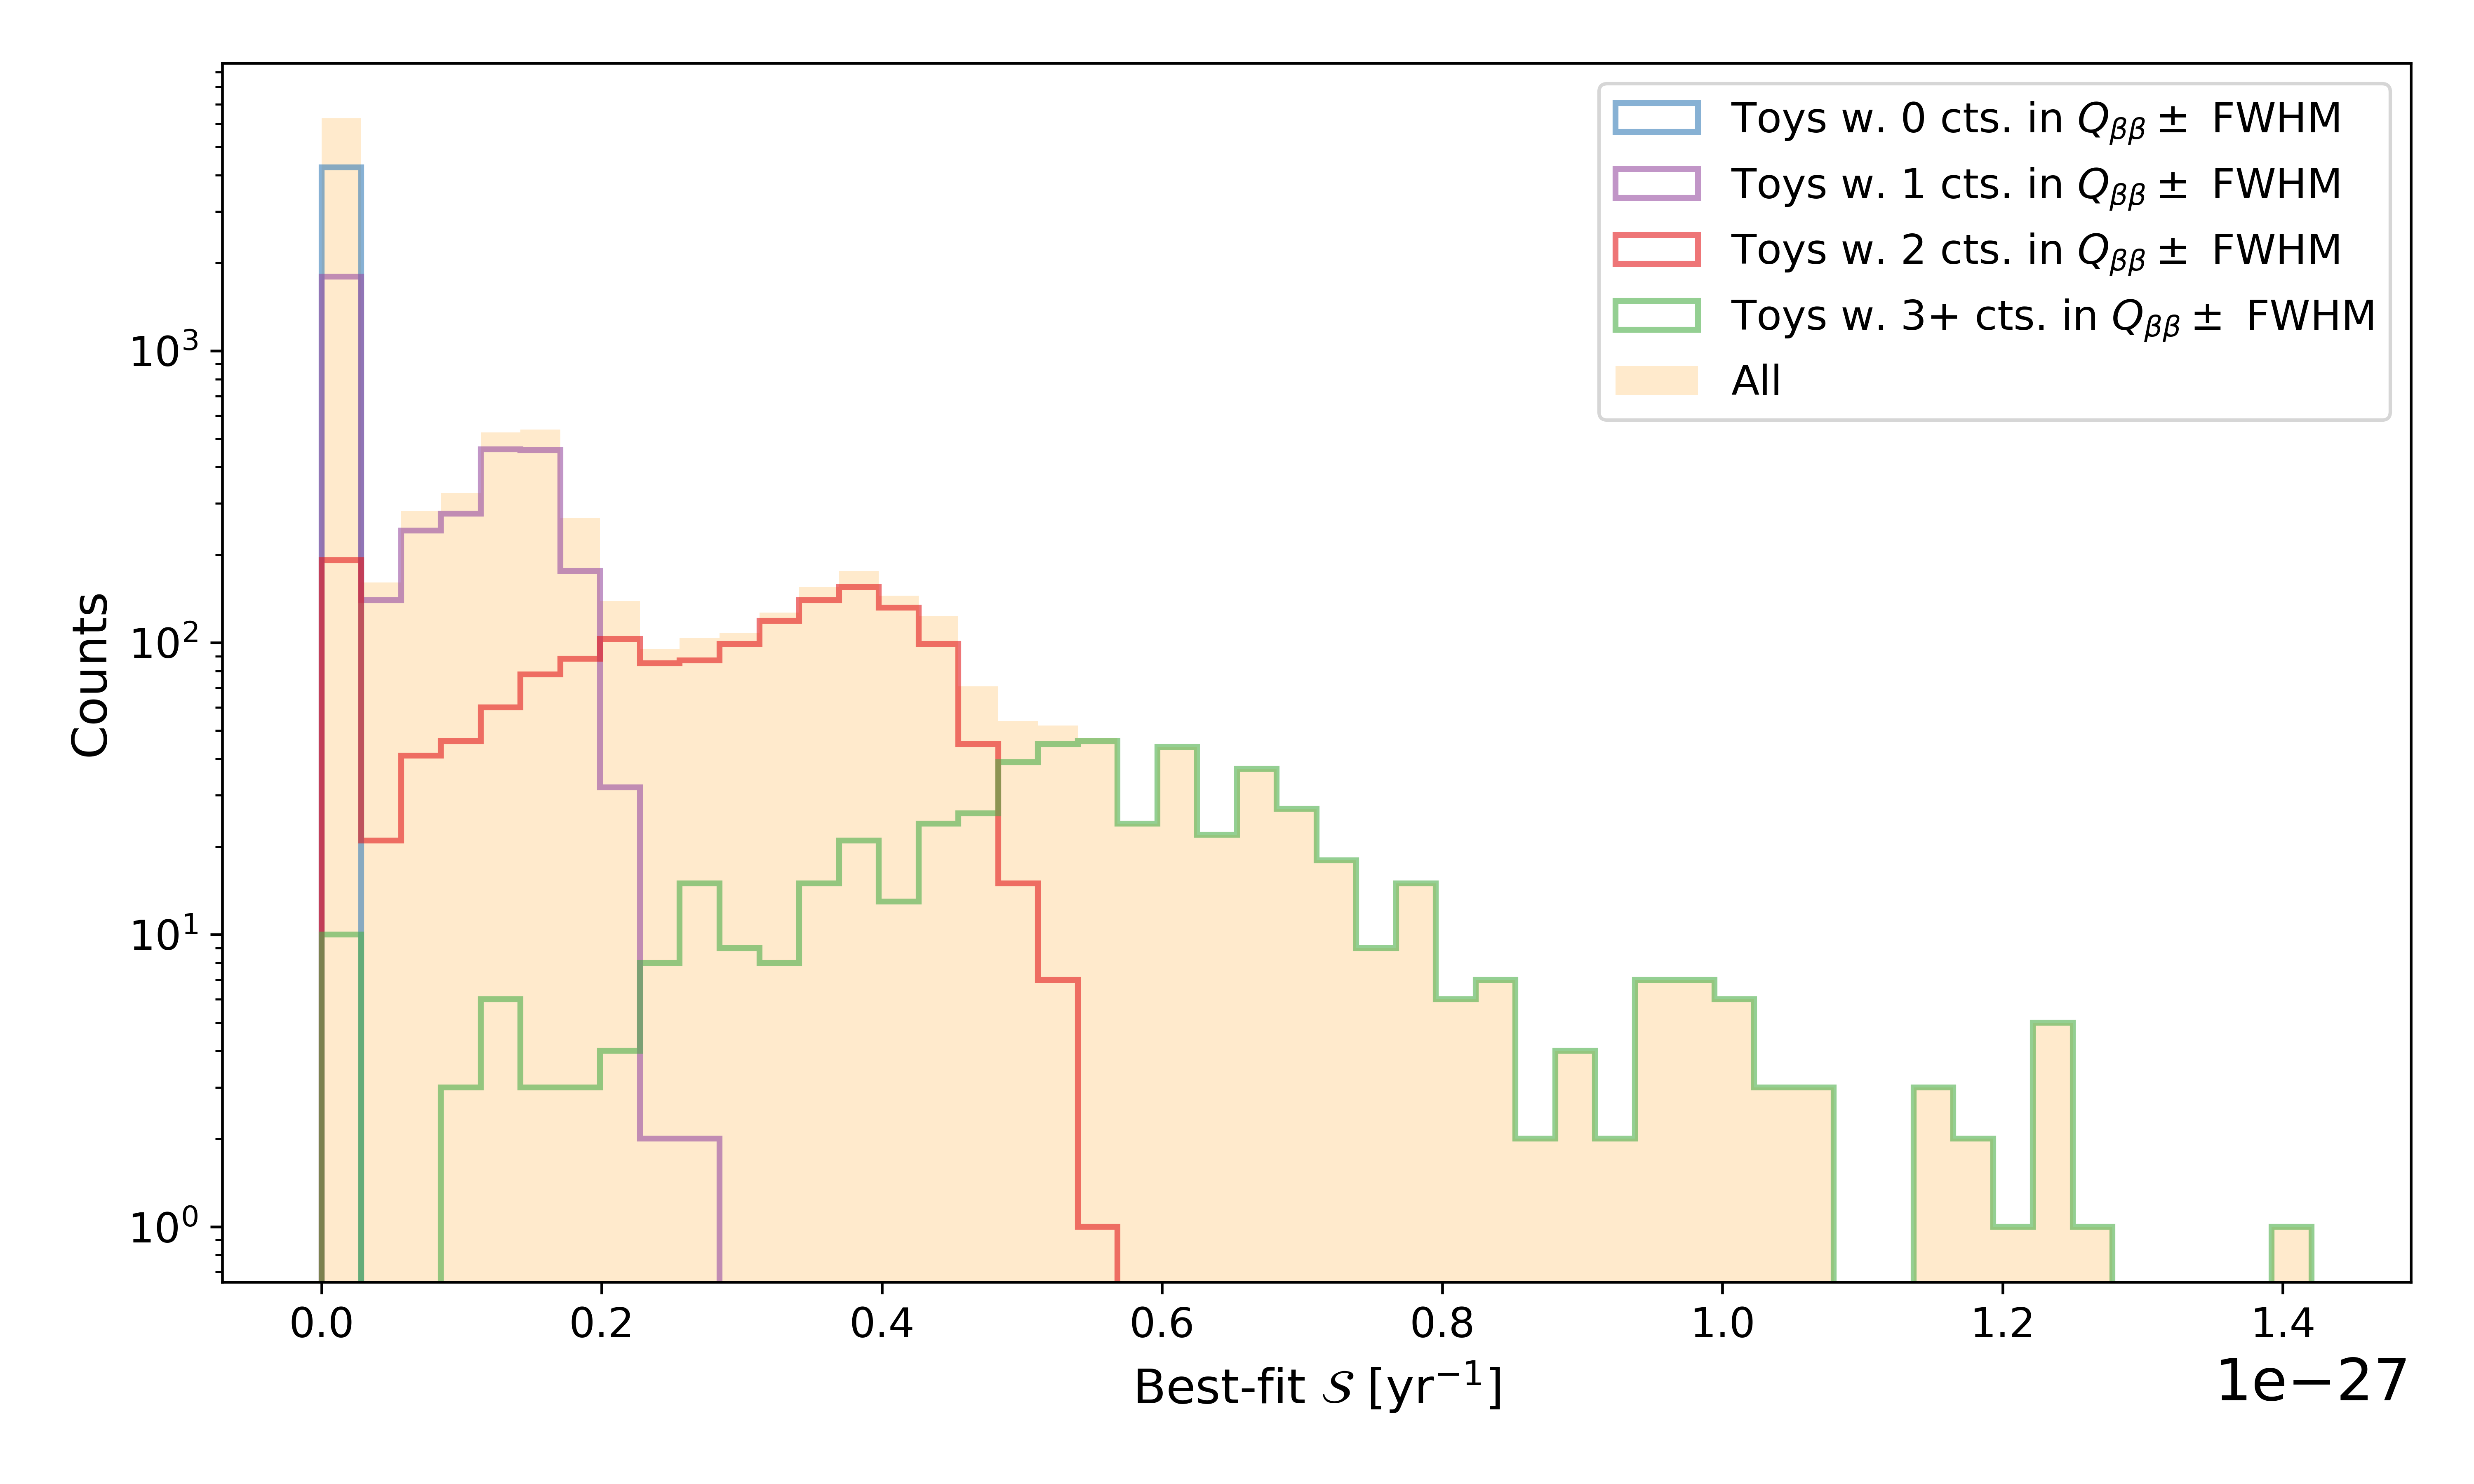
\includegraphics[width=0.9\linewidth]{figures/06_sensitivity/Signal_fits_per_ROIcount.png}
\caption{Distribution of best-fit $\mathcal{S}$ from A/E-based MCMC fits, grouped by the number of events observed within $Q_{\beta \beta} \pm$~FWHM. Modes at non-zero $\mathcal{S}$ are associated with datasets containing one or more background events near the region of interest.} 
\label{fig:S_fit_per_ROIcount}
\end{figure}


This analysis is performed using ZeroNuFit.jl~\cite{dixon_legend-expzeronufitjl_2025}, a specialized Bayesian analysis tool built on the Bayesian Analysis Toolkit (BAT.jl)~\cite{schulz_batjl_2021}. ZeroNuFit.jl implements extended unbinned maximum likelihood fits tailored for $0 \nu \beta \beta$ decay searches, allowing flexible modeling of both signal peaks and background components. The statistical framework we used is further described in~\cite{lnote_25001}. 



\subsection{Results of the Bayesian analysis}

To assess the physics reach of the Transformer PSD strategy, in comparison with the conventional A/E method, a Bayesian half-life sensitivity analysis for the $0 \nu \beta \beta$ decay was performed separately for each PSD method. Using the LEGEND-200 goal exposure and background index, the final $0 \nu \beta \beta$ decay half-life sensitivity of LEGEND-200 was estimated, with the PSD efficiencies treated as Gaussian-distributed nuisance parameters in the fit.  

For each toy dataset, we extracted the 90\% one-sided upper CI limit on the signal half-rate, $\mathcal{S}_{90}$. Its distribution over all toys reflects the expected sensitivity of the experiment: the median, $\tilde{\mathcal{S}}_{90}$ defines the central value, and the 68\% credible interval quantifies the associated uncertainty. This procedure incorporates both statistical fluctuations and systematic uncertainties, as the signal detection efficiency and energy resolution are sampled from their priors and marginalized over in each fit. 
Since the signal half-rate is inversely proportional to the half-life, its median and $68$\% CI range can be directly translated into a median and $68$\% CI range for the $0 \nu \beta \beta$ decay half-life. By comparing the half-lives derived from each PSD method, we can evaluate their respective impacts on the exclusion sensitivity.

\begin{table}
\centering
\caption{Comparison of PSD efficiency, resulting signal half-rate limits and half-life limits for the Transformer and A/E methods.}
\renewcommand{\arraystretch}{1.5}
\begin{tabular}{|| c | c | c | c ||}
	\hline
 	\textbf{Method} & \textbf{PSD eff. [\%]}  & $\boldsymbol{\tilde{\mathcal{S}}_{90} \; [10^{-28} \,\mathrm{yr}^{-1}]}$ & $\mathbf{T^{0 \nu}_{1/2} [10^{27} \, yr]}$ \\
 	\hline
	A/E & $84.3 \pm 0.5$ & $8.23^{+3.65}_{-1.76}$ & $1.22^{+0.33}_{-0.37}$ \\
 	\hline
 	Transformer & $86.7 \pm 1.3$ & $8.00^{+3.42}_{-1.71}$ & $1.25^{+0.34}_{-0.37}$\\
	\hline
\end{tabular}
\label{tab:Results}
\end{table}

All results are summarized in table~\ref{tab:Results}, and the signal half-rate $90$\% CI upper limits distributions are shown in figure~\ref{fig:Results_S_hist}. For the A/E cut, we obtain:

\begin{equation}
    \mathcal{S} = 8.23^{+3.65}_{-1.76} \times 10^{-28} 
\end{equation}

With the definition $T^{0 \nu}_{1/2} = 1/\mathcal{S}$, this translates to a Bayesian 90\% credible lower bound on the $0 \nu \beta \beta$ decay half-life of:

\begin{equation}
    T_{1/2} > 1.22^{+0.33}_{-0.37} \times 10^{27} \; \mathrm{yr}
\end{equation}

Similarly, using the Transformer-based PSD efficiency, the Bayesian analysis yields:

\begin{equation}
    \mathcal{S} < 8.00^{+3.42}_{-1.71} \times 10^{-28} \; \mathrm{yr}^{-1} 
\end{equation}

and

\begin{equation}
    T_{1/2} > 1.25^{+0.34}_{-0.37} \times 10^{27} \; \mathrm{yr} 
\end{equation}

\begin{figure}
\centering
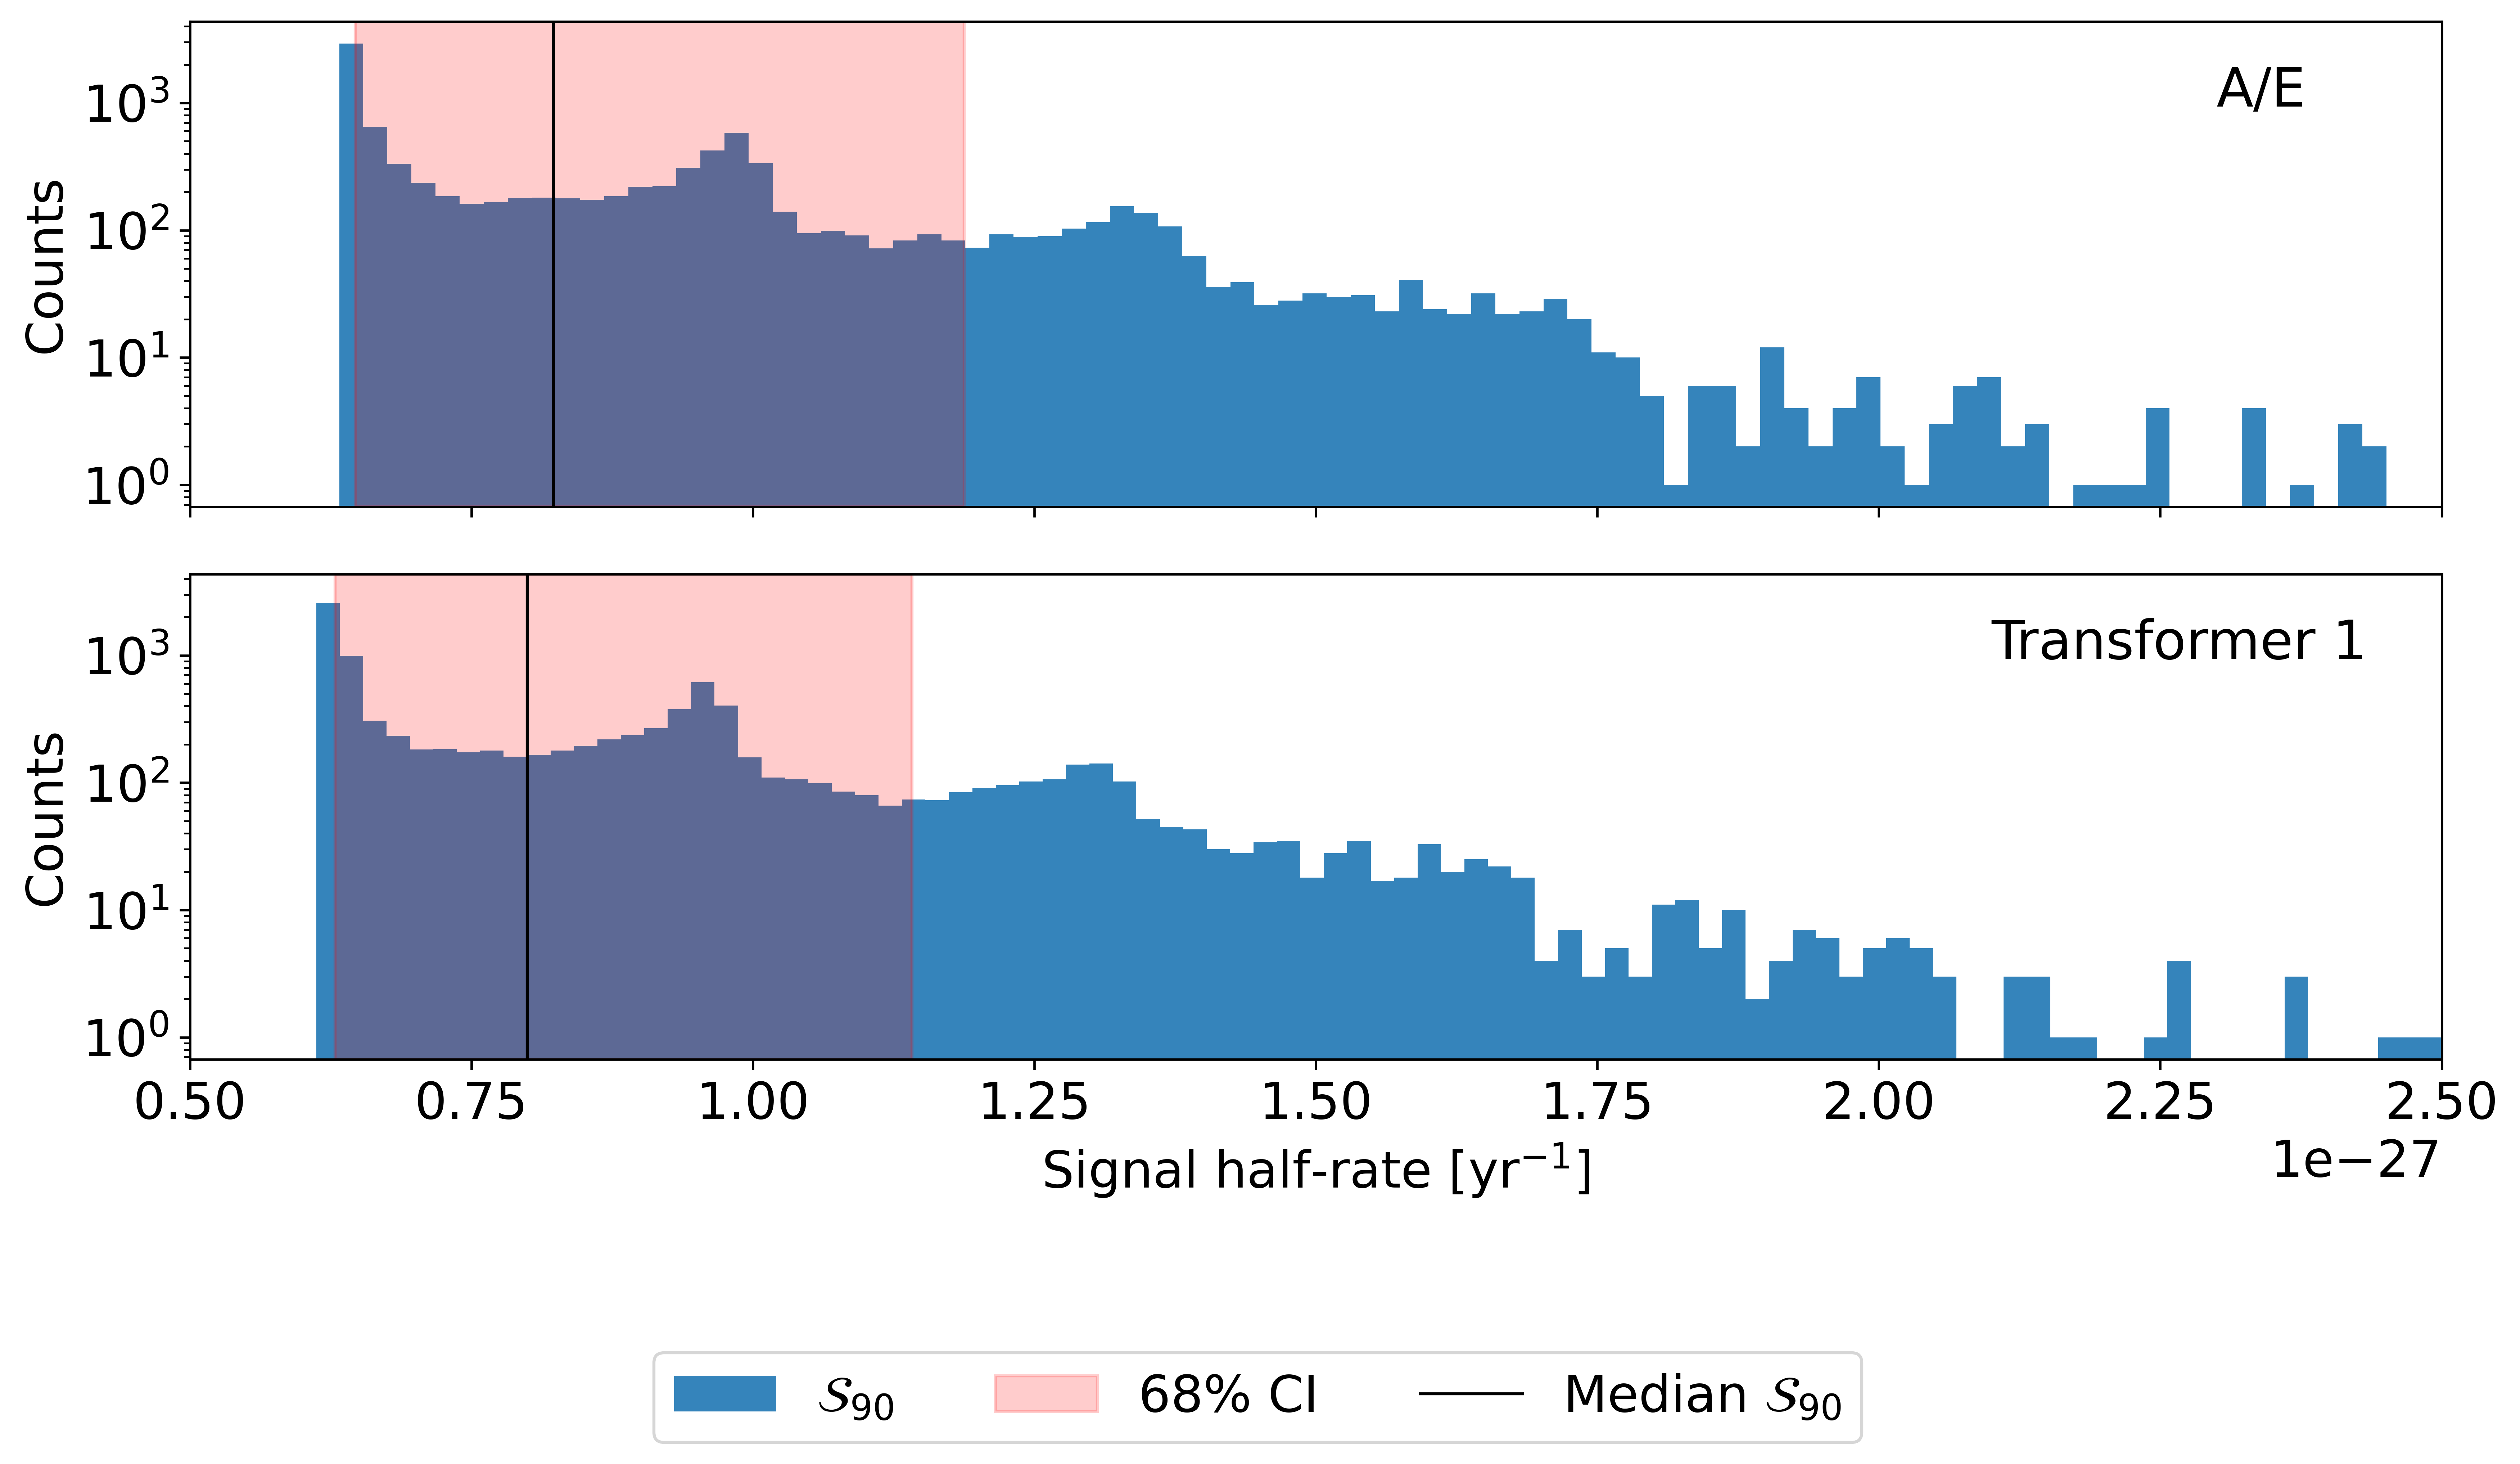
\includegraphics[width=0.9\linewidth]{figures/06_sensitivity/Results_S_histogram_1000kgyr.png}
\caption{Distribution of 90\% upper credible limits on the signal half-rate $\mathcal{S}$ obtained from 10'000 toy Monte Carlo simulations under the background-only hypothesis. The upper plot shows results obtained from the A/E cut, the lower from the Transformer-based PSD cut. The Transformer method achieved a slightly improved sensitivity, reflected by the lower median. } 
\label{fig:Results_S_hist}
\end{figure} 


%--------------------- Conclusion & Outlook ---------------------
\clearpage
\section{Conclusion and outlook} 
\label{sec:07_conculsion}
In this work, a Transformer-based approach to pulse shape discrimination was developed for the LEGEND-200 experiment, aiming to improve the separation of signal-like events from background noise in the search for neutrinoless double beta decay.
The model developed achieved a PSD efficiency of $(86.7 \pm 1.3)$\% at $Q_{\beta \beta}$, which agrees with the conventional A/E method $(84.3 \pm 0.5)$\%. A two-sided test of the difference between Transformer-based PSD efficiency and A/E yields $p = 0.08$, indicating that the observed 2.4\% difference is not statistically significant at the 5\% level.
While the Transformer-based method demonstrates a higher central efficiency, it also exhibits a larger uncertainty. This broader uncertainty reflects not just statistical variation, but also contributions from model variance and possible sensitivity to detector-specific features. In contrast to the A/E method, which is calibrated per detector and period, the Transformer is trained globally across all detectors and periods. This choice enables cross-detector generalization but can also introduce performance fluctuations when the training data does not sufficiently capture detector-to-detector variation. The elevated uncertainty may therefore indicate a trade-off between generalization and robustness, and suggests the need for better-balanced training data. 

A Bayesian $0 \nu \beta \beta$ decay sensitivity analysis yields signal half-rate limits of $\mathcal{S} = 8.23^{+3.65}_{-1.76} \times 10^{-28}$ (A/E) and $\mathcal{S} < 8.00^{+3.42}_{-1.71} \times 10^{-28} \; \mathrm{yr}^{-1}$ (Transformer), if we assume the LEGEND-200 design goals are reached (background index $2 \times 10^{-4}$ counts/(keV$\cdot$kg$\cdot$yr), exposure $1000 \;\mathrm{kg \cdot yr}$). Both Transformer-based method ($T^{0 \nu}_{1/2} = 1.25^{+0.34}_{-0.37} \times 10^{27}$yr) and conventional A/E ($T^{0 \nu}_{1/2} = 1.22^{+0.33}_{-0.37} \times 10^{27}$yr) cuts agree within uncertainty, validating the Transformer-based approach as a viable alternative for pulse shape discrimination. 

Although a significant sensitivity improvement was not yet achieved, these results demonstrate that machine-learning techniques, particularly Transformer architectures, can achieve performance comparable to well-established PSD methods refined and optimized extensively over many years.
However, the Transformer introduces additional computational overhead, since training requires labeled datasets generated using conventional methods. This cost is largely a one-time expense, as the training would be repeated or updated only when detector conditions change. Once trained, classification of new waveforms is relatively fast, so the computational cost is amortized over large amounts of data. 
With further development, the Transformer-based PSD method shows promise for enhancing sensitivity in rare-event searches, though several aspects still require improvement.

First, the quality and consistency of training data should be improved by applying stricter data cleaning procedures, more rigorous detector selection, and better data balance (across energies and detectors) to increase the model's robustness and reduce sensitivity to unwanted features. 

Second, further investigation is needed into the $^{56}$Co waveforms, as their inclusion in the training set led to poor generalization of events below 1.5~MeV, resulting in reduced PSD performance in the $2 \nu \beta \beta$ decay energy region. This again highlights the need for improved training data, particularly in terms of data quality and data balance. 

Third, incorporating pulse shape simulations and domain adaptation techniques could help mitigate detector-specific effects and improve the model performance across a larger energy region.  

If Transformer-based (or other ML-based) PSD methods continue to demonstrate competitive performance, future work should also address their integration into the experiment's digital signal processing pipeline. 
As LEGEND progresses towards its ton-scale goals, deep learning-based PSD methods may become a critical component in maximizing the experiment's sensitivity to rare physics beyond the Standard Model. 
Their scalability could not only enhance event classification but also enable advanced techniques such as unsupervised anomaly detection, offering new avenues for discovery. 

%--------------------- Acknowledgements ---------------------
\clearpage
\pagestyle{plain}
\begin{center}
\section*{Acknowledgements}
\end{center}
\textit{
I would like to thank the LEGEND group at the University of Zurich for their support throughout this project. 
I am especially grateful to Aravind Remesan Sreekala and Gloria Senatore for their help with detector simulations, to Giovanna Saleh for her support on pulse shape simulations, to Dr. Francesco Piastra for his guidance on detector physics, and to Dr. Sofia Calgaro for her invaluable support with the Bayesian sensitivity analysis. \\
I am grateful to Prof. Laura Baudis for welcoming me into her group and for her guidance and insightful feedback at key stages of the project, as well as to Dr. Marta Babicz for her guidance and supervision. I also thank Prof. Laura Baudis, Dr. Marta Babicz, and Dr. Sofia Calgaro for their feedback and suggestions, which helped improve this thesis.
Finally, I would like to thank my partner and my parents for their support and encouragement throughout my studies.
}



%--------------------- Bibliography ---------------------
\clearpage
\pagestyle{plain} % or 'empty' if you want no header/footer at all
\printbibliography
\end{document}
